%& -output-directory=./build -aux-directory=./build
\documentclass[11pt,notitlepage,twoside,BCOR=8.25mm,headsepline,numbers=noendperiod,DIV=14]{scrbook} %numbers=endperiod,titlepage,

% PDF/A compliance?
%\usepackage[a-1b]{pdfx} 

%\usepackage{multicolumn}
%% Font setup
\usepackage[default]{gillius}
%\usepackage{glossaries}

\usepackage{cite}
\usepackage{lineno}
\usepackage{mathpazo}
%\usepackage{helvet}%      Choose default sans serif
%\usepackage{gillius}%      Choose default sans serif
\usepackage{sectsty}%     Change style of headings (should precede section redefinitions below)  
\allsectionsfont{\sffamily}% Set sans serif for all headings
%\allsectionsfont{\fontfamily{lmr}\selectfont}% Set sans serif for all headings

\usepackage[T1]{fontenc}
\usepackage[utf8]{inputenc}
\usepackage[english]{babel}

% Setup commands
\addtokomafont{disposition}{\boldmath}

% allow using fonts of any size
%\usepackage{lmodern}

%\usepackage{libertine}

% additional characters for franch
\usepackage[utf8]{inputenc}
%\usepackage[T1]{fontenc}
\usepackage{bold-extra}

%\usepackage[]{inputenc}
\usepackage{amsmath}
\usepackage{amsfonts}
\usepackage{mathrsfs}
\usepackage{amssymb}
%\usepackage[amssymb]{SIunits}
%\usepackage{siunitx}

\usepackage{xspace}
\usepackage{wrapfig}

\usepackage{upgreek}
\usepackage{graphicx}
\usepackage[section]{placeins}%automatic \FloatBarrier between sections
\usepackage{placeins}

\usepackage{feynmf}

\usepackage{booktabs}
\usepackage[usenames,dvipsnames]{xcolor}

%\usepackage[figuresright]{rotating}
\usepackage{rotating}
\usepackage{array}

\usepackage{fp}

\usepackage{cprotect}

\usepackage{cite}
%\bibliographystyle{fra_hannes_lucas_unsrt.bst}

\usepackage{tabularx}
%\usepackage{footnote}
%\makesavenoteenv{tabular}
%\makesavenoteenv{table}

\usepackage{pdflscape}

 %CHANGE for online version
\usepackage[colorlinks,
pdfpagelabels,
pdfstartview = FitH,
bookmarksopen = false,
bookmarksnumbered = true,
linkcolor = black,
plainpages = false,
hypertexnames = false,
urlcolor = black,
citecolor = black] {hyperref}

\usepackage{setspace}

\usepackage{pennames-ital}
\usepackage{ptdr-definitions}
% Custom hyphentation
\hyphenation{brems-strah-lung}
\hyphenation{fi-gure}
%% dummy text producer
\usepackage{lipsum}

%\linenumbers

%%%%%%%%%%%%%%%%%%%%%%%%%%%%%%%%%
% Fancy chapter heading
%%%%%%%%%%%%%%%%%%%%%%%%%%%%%%%%%
%\usepackage[T1]{fontenc}
%\usepackage{titlesec, blindtext, color}
%\definecolor{gray75}{gray}{0.75}
%\newcommand{\hsp}{\hspace{20pt}}
%\titleformat{\chapter}[hang]{\Huge\bfseries}{\thechapter\hsp\textcolor{gray75}{|}\hsp}{0pt}{\Huge\bfseries}
%%%%%%END-CHAP-HEADING%%%%%%%%%%%


%%%%%%%%%%%%%%%%%%%%%%%%%%%%%%%%%
% Abstract environment for book
%%%%%%%%%%%%%%%%%%%%%%%%%%%%%%%%%
\makeatletter
\if@titlepage
  \newenvironment{abstract}[1][Abstract]{%
      \pagestyle{empty}
      \null\vfil
      \@beginparpenalty\@lowpenalty
      \begin{center}%
        \large \bfseries #1
        \@endparpenalty\@M
      \end{center}}%
     {\par\vfil\null\thispagestyle{empty}}
\else
  \newenvironment{abstract}[1][Abstract]{%
      \if@twocolumn
        \section*{#1}%
      \else
	\pagestyle{empty}
	\null\vfil
	\@beginparpenalty\@lowpenalty
        \small
        \begin{center}%
          {\large \bfseries #1\vspace{-.5em}\vspace{\z@}}%
          \@endparpenalty\@M
        \end{center}%
        \quotation
      \fi}
      {\if@twocolumn\else\vfil\null\endquotation\thispagestyle{empty}\fi}
\fi
\makeatother
%%%%%%END-ABSTRACT%%%%%%%%%%%%%%%
%\listfiles

%%%%% FANCY CHAPTER HEADING

%% now change the chapter style
%% load up the quotchap package
%\RequirePackage[utopia]{quotchap}
%\RequirePackage[palatino]{quotchap}
% make the quotation appear next to the chapter number
%\renewcommand\chapterheadstartvskip{\vspace*{-3.5\baselineskip}}
%\renewcommand*\chapterheadendvskip{\vspace{1.2\baselineskip}}

%%%% FNCYchap
\usepackage[PetersLenny]{fncychap}
%\ChTitleVar{\huge\bfseries\fontfamily{palatino}}
\ChTitleVar{\huge\bfseries\rmfamily}
%\ChTitleVar{\huge\fontfamily{palatino}}

%%% CHANGE vspace in FNCYCHAP
\makeatletter
\def\@makechapterhead#1{%
%	\vspace*{50\p@}%
	\vspace*{10\p@}%
	{\parindent \z@ \raggedright \normalfont
		\ifnum \c@secnumdepth >\m@ne
		\if@mainmatter%%%%% Fix for frontmatter, mainmatter, and backmatter 040920
		\DOCH
		\fi
		\fi
		\interlinepenalty\@M
		\if@mainmatter%%%%% Fix for frontmatter, mainmatter, and backmatter 060424
		\DOTI{#1}%
		\else%
		\DOTIS{#1}%
		\fi
	}}

\def\@makeschapterhead#1{%
%	\vspace*{50\p@}%
%	\vspace*{5\p@}%
	{\parindent \z@ \raggedright
		\normalfont
		\interlinepenalty\@M
		\DOTIS{#1}
%		\vskip 40\p@
		\vskip 5\p@
	}}	
\makeatother

%% package for toc at the
%% beginning of chapters
\usepackage[nohints]{minitoc}

%\usepackage{titlesec}
%\titleformat{\paragraph}[runin]{\normalfont\large\bfseries}{\theparagraph}{1em}{}
%\titleformat{\chapter}[runin]{\normalfont\large\bfseries}{\thechapter}{1em}{}
\let\oldParagraph\paragraph
\renewcommand{\paragraph}[1]{\oldParagraph{#1}\mbox{} \vspace{2mm} \\}

\usepackage{tikz}
\usepackage[percent]{overpic}
\usetikzlibrary{shadows}

%\setlength{\itemsep}{0pt}
\usepackage[inline]{enumitem}[2011/09/28]
\newcommand{\localtextbulletone}{\textcolor{black}{\raisebox{-0.38ex}{\tikz\node[drop shadow={
                        top color=gray,
                        bottom color=white,
                        fill=gray,
                        shadow scale=0.53,
                        %opacity=0.2,
                        shadow xshift=0pt,
                        shadow yshift=0pt
                        }]
                {\rule{.75ex}{.4ex}};}}}
%\renewcommand{\labelitemi}{\hspace{\labelsep}\localtextbulletone}
\newcommand{\myitem}[1][{}]{\item\textbf{#1}}
\newenvironment{mylist}
	{\begin{itemize}[itemsep=0pt,topsep=4pt]}{\end{itemize}\vspace{.1\baselineskip}}

%\setlength{\parindent}{15pt}
%\renewcommand\descriptionlabel[1]{\hspace{\labelsep} \textbf{\labelitemi\enskip #1}}

%%%%%%%%%%%%%%%%%%%%%%%%%%%%%%%%%
% Useful Commands
%%%%%%%%%%%%%%%%%%%%%%%%%%%%%%%%%
\let\oldMinitoc\minitoc
\renewcommand{\minitoc}{\oldMinitoc\vspace{4mm}}

\newcommand{\blankpage}{\newpage\thispagestyle{empty}\mbox{}\newpage}
\newcommand{\myapprox}{\ensuremath{\sim}}
%%%%%%END-COMMANDS%%%%%%%%%%%%%%%

\frenchspacing

%%%%%%%%%%%%%%%%%%%%%%%%%%%%%%%%%%%%%%%
% Headings, footings, section titles
%%%%%%%%%%%%%%%%%%%%%%%%%%%%%%%%%%%%%%%

\usepackage{scrpage2}
\pagestyle{scrheadings}
\setheadsepline{.8pt}

%\renewcommand{\chaptermark}[1]{\markboth{\MakeUppercase{\chaptername\ \thechapter.\ #1}}{}}
\renewcommand*{\chaptermark}[1]{\markboth{\large{\thechapter\ #1}}{}}
\renewcommand*{\sectionmark}[1]{\markright{\large{\thesection\ #1}}{}}

% \setkomafont{chapter}{\normalfont\bfseries\fontsize{16}{21}\selectfont\scshape}
% \setkomafont{section}{\normalfont\fontsize{13}{15.5}\selectfont}
% \setkomafont{subsection}{\normalfont\slshape\fontsize{13}{15.5}\selectfont}
% \setkomafont{paragraph}{\normalfont\slshape\fontsize{13}{15.5}\selectfont}
% \setkomafont{subparagraph}{\normalfont\slshape\fontsize{13}{15.5}\selectfont}


\usepackage{multirow}
\newcommand\T{\rule{0pt}{2.6ex}}       % Top strut
\newcommand\B{\rule[-1.5ex]{0pt}{0pt}} % Bottom strut

\usepackage{array}
\newcolumntype{L}[1]{>{\raggedright\let\newline\\\arraybackslash\hspace{0pt}}m{#1}}
\newcolumntype{C}[1]{>{\centering\let\newline\\\arraybackslash\hspace{0pt}}m{#1}}
\newcolumntype{R}[1]{>{\raggedleft\let\newline\\\arraybackslash\hspace{0pt}}m{#1}}

\usepackage{tikz}
\definecolor{myRed}{RGB}{204, 0, 0}

\usepackage{nicefrac}

\usepackage{multicol}
%\usepackage{glossary-mcols}
\setlength{\columnsep}{25pt}


\usepackage{caption}
\usepackage{subcaption}
\addto\captionsenglish{\renewcommand{\figurename}{Fig.}}

% \makeatletter
% \renewenvironment{thebibliography}[1]
%      {\begin{multicols}{2}[\section*{\refname}]%
%       \@mkboth{\MakeUppercase\refname}{\MakeUppercase\refname}%
%       \list{\@biblabel{\@arabic\c@enumiv}}%
%            {\settowidth\labelwidth{\@biblabel{#1}}%
%             \leftmargin\labelwidth
%             \advance\leftmargin\labelsep
%             \@openbib@code
%             \usecounter{enumiv}%
%             \let\p@enumiv\@empty
%             \renewcommand\theenumiv{\@arabic\c@enumiv}}%
%       \sloppy
%       \clubpenalty4000
%       \@clubpenalty \clubpenalty
%       \widowpenalty4000%
%       \sfcode`\.\@m}
%      {\def\@noitemerr
%        {\@latex@warning{Empty `thebibliography' environment}}%
%       \endlist\end{multicols}}
% \makeatother
\widowpenalty=2000
\clubpenalty=2000
\displaywidowpenalty=300
\raggedbottom

\interlinepenalty = 10
\binoppenalty=1000

\DeclareMathSizes{10.95}{10.95}{7}{6}
\input{Aux/CrossSections}
\input{Aux/cutFlows.tex}
\input{Aux/testUnivers.tex}
%% images directorty
\graphicspath{{figures/}}
\usepackage[outdir=figures/]{epstopdf}
%\epstopdfsetup{outdir=figures/}
%% line numbers
\usepackage{lineno}
%\linenumbers

%%%%%%%%%%%%%%%%%%%%%%%%%%%%%%%%%
% Load Abbreviations
%%%%%%%%%%%%%%%%%%%%%%%%%%%%%%%%%
\usepackage{multicol}

\usepackage{longtable}
\usepackage[nomain,acronym, xindy={glsnumbers=false}, 
  toc, %section, %glossary in the toc as sections
  nonumberlist,  %to suppress the location list within the glossary
  sort=standard
  ]{glossaries}
\usepackage{glossary-mcols}
  
%\usepackage[acronym]{glossaries}  
%\usepackage[nonumberlist]{glossaries} %to suppress the location list within the glossary
\renewcommand*{\glspostdescription}{} %to suppress the dot at the end of the glossary description
\let\oldgls\gls
\renewcommand*\gls{\protect\oldgls}

\newcommand {\cf}{\mbox{cf.}\xspace} 
\newcommand {\wrt}{\mbox{w.r.t.}\xspace}

\newcommand {\mtau}{{\ensuremath{\Pgt}}\xspace} 
\newcommand {\mtauh}{{\ensuremath{\Pgt_h}}\xspace} 

\newcommand {\isorel}{{\ensuremath{\mathrm{Iso}_{\mathrm{rel}}\xspace}}}
\newcommand {\miniiso}{{\ensuremath{\mathrm{I}_{\mathrm{mini}}\xspace}}}

 \newglossarystyle{mystyle}{%
  \renewenvironment{theglossary}
    {\tablehead{}\tabletail{}%
     \begin{supertabular}{@{}>{\bfseries}lp{\textwidth}}}%
     %p{\glsdescwidth}}}%
     %p{\glspagelistwidth}}}%
    {\end{supertabular}}%
  \renewcommand*{\glossaryheader}{}%
  \renewcommand*{\glsgroupheading}[1]{}%
  \renewcommand*{\glossaryentryfield}[5]{%
    %\glsentryitem{##1}\glstarget{##1}{##2} & ##3 & ##5\\}%
    ##4 & \glsentryitem{##1}\glstarget{##1}{##2}\\}%
  \renewcommand*{\glossarysubentryfield}[6]{%
     &
     \glssubentryitem{##2}%
     \glstarget{##2}{\strut}##4 & ##6\\}%
  \renewcommand*{\glsgroupskip}{ & \\}%
}
 
\newglossarystyle{mmystyle}{%
  \setglossarystyle{mystyle}%
  \renewenvironment{theglossary}%
    {%
     \begin{multicols}{2}
     \setlength{\parindent}{0pt}%
     \setlength{\parskip}{0pt plus 0.3pt}%
     }%
    {\end{multicols}}%
}
 
\makeatletter
  %%
  %% modification of mcolalttree;
  %% everything taken verbatim from mcolalttree, exception indicated
  %%
  \newglossarystyle{mymcolalttree}{%
    \glossarystyle{alttree}%
    \renewenvironment{theglossary}%
      {%
        \begin{multicols}{2}%
         \setlength{\parindent}{0pt}%
     \setlength{\parskip}{0pt plus 0.3pt}%
      }%
      {%\end{supertabular}
      \par\end{multicols}}%
      %\renewcommand*{\glsgroupheading}[1]{\begin{description}[style=multiline,align=left]}
    \renewcommand{\glossaryentryfield}[5]{%
      \begin{description}[style=multiline,align=left]
      \item[##4:] \glstarget{##1}{##2}%
      %\item[##4:] \glsentrylong{##1}%
      \end{description}\vspace{-.5cm}
    }%
   \renewcommand*{\glsgroupskip}{\mbox{ }\\ \vspace{-0.3cm}}%
  }%
\makeatother
  
 
\renewcommand{\acrfullformat}[2]{#1~(#2)} %abbreviation not on a new line
%\let\glsdisplayold\glsdisplay
%\renewcommand{\glsdisplay}{gasgasdgasdfgewrgaerd\glsdisplayold}
%\defglsdisplay[main]{adfasd#1}
%\renewcommand*{\glsdisplayfirst}[4]{\textcolor{blue}{#1}#4}
%\SetCustomDisplayStyle

\renewcommand{\CustomAcronymFields}{%
   name={\the\glslongtok},%
   symbol={\the\glsshorttok},%
   text={\the\glsshorttok},%
   first={{\the\glslongtok}~(\the\glsshorttok)},%
   plural={{\the\glsshorttok}\noexpand\acrpluralsuffix},%
   firstplural={\the\glslongtok\noexpand\acrpluralsuffix~(\the\glsshorttok)},%
   description={}
 }
%\renewcommand*{\SetCustomDisplayStyle}[1]{%
% \defglsdisplayfirst[#1]{##1##4
% }%
% \defglsdisplay[#1]{~##1##4}%
% }
 
% stops gaps between groups
\renewcommand{\glsgroupskip}{} 
 
\SetCustomStyle
\makeglossaries

% 
% \renewcommand*{\SetCustomDisplayStyle}[1]{%
%   \defglsdisplayfirst[#1]{##1##4\protect\footnote{%
%   \glsentrylong{\glslabel}: ##2%
%   }}
%   \defglsdisplay[#1]{##1##4}%
% }
% 
% \SetCustomDisplayStyle


% abbreviations:

\newacronym[sort=macho]{macho}{MACHO}{massive astrophysical compact halo object} 
\newacronym[sort=cmb]{cmb}{CMB}{Cosmic Microwave Background}

\newacronym[sort=ckm]{ckm}{CKM}{Cabibbo--Kobayashi--Maskawa}
\newacronym[sort=pmns]{pmns}{PMNS}{Pontecorvo--Maki--Nakagawa--Sakato}
\newacronym[sort=gut,firstplural=Grand Unified Theories~(GUT)]{gut}{GUT}{Grand Unified Theory}


\newacronym[sort=ued]{ued}{UED}{Universal Extra Dimensions}
\newacronym[sort=ltp]{ltp}{LTP}{lightest T-odd particle}
\newacronym[sort=lkp]{lkp}{LKP}{lightest Kaluza-Klein particle}
%\newacronym[sort=ewpt]{expt}{EWPT}{electroweak precision test}

\newacronym[sort=me]{me}{ME}{matrix element}
\newacronym[sort=ps]{psh}{PS}{parton shower}

\newcommand{\atlas}{\textsc{ATLAS}\xspace}
\newcommand{\pythia}{\textsc{Pythia}\xspace}
\newcommand{\herwig}{\textsc{Herwig}\xspace}
\newcommand{\madgraph}{\textsc{MadGraph}\xspace}
\newcommand{\powheg}{\textsc{Powheg}\xspace}
\newcommand{\amcatnlo}{\textsc{aMC@NLO}\xspace}
\newcommand{\tauola}{\textsc{Tauola}\xspace}
\newcommand{\prospino}{\textsc{Prospino}\xspace}

\newacronym[sort=geant]{geant}{GEANT4}{GEometry ANd Tracking}


\newacronym[sort=qps]{qps}{QPS}{Quench Protection System}

\newacronym[sort=qed]{qed}{QED}{quantum electrodynamics}
\newacronym[sort=qcd]{qcd}{QCD}{quantum chromodynamics}
\newacronym[sort=as]{alphas}{\ensuremath{\alpha_{s}}}{strong coupling constant}

\newacronym[sort=susy]{susy}{SUSY}{Supersymmetry}
\newcommand{\susy}{\gls{susy}\xspace}
\newacronym[sort=lsp]{lsp}{LSP}{lightest supersymmetric particle}
\newacronym[sort=ewsb]{ewsb}{EWSB}{electroweak symmetry breaking}


\newacronym[sort=mssm]{mssm}{MSSM}{Minimal Supersymmetric extension of the Standard Model}
\newacronym[sort=cmssm]{cmssm}{cMSSM}{constrained MSSM}
\newacronym[sort=pmssm]{pmssm}{pMSSM}{phenomenological MSSM}
\newacronym[sort=sms,plural=SMS,firstplural=simplified model spectra~(SMS)]{sms}{SMS}{simplified model spectra}
\newacronym[sort=mc]{mc}{MC}{Monte Carlo}
\newacronym[sort=lo]{lo}{LO}{leading order}
\newacronym[sort=nlo]{nlo}{NLO}{next-to-leading order}

\newcommand{\linac}{LINAC1\xspace}
\newcommand{\linacII}{LINAC2\xspace}
\newcommand{\linacIII}{LINAC3\xspace}
\newcommand{\linacIV}{LINAC4\xspace}

\newacronym[sort=pd]{pd}{PD}{Primary Dataset}
% Lumi
\newacronym[sort=pcc]{pcc}{PCC}{Pixel Cluster Counting}
\newacronym[sort=plt]{plt}{PLT}{Pixel Luminosity Telescope}
\newacronym[sort=bcm]{bcm}{BCM1f}{Fast Beam Condtions Monitore}

\newacronym[sort=psb]{psb}{PSB}{PS Booster}
\newacronym[sort=ps]{ps}{PS}{Proton Synchrotron}
\newacronym[sort=sps]{sps}{SPS}{Super Proton Synchrotron}

\newacronym[sort=ibs]{ibs}{IBS}{intra beam scattering}

\newacronym[sort=lhc]{lhc}{\textsc{LHC}}{Large Hadron Collider} \newcommand{\lhc}{\gls{lhc}\xspace}
\newacronym[sort=hllhc]{hllhc}{HL-LHC}{High-Luminosity LHC}

\newacronym[sort=ls1]{ls1}{LS1}{first Long Shutdown}
\newacronym[sort=ls2]{ls2}{LS2}{second Long Shutdown}

\newacronym[sort=ilc]{ilc}{ILC}{International Linear Collider}
\newacronym[sort=clic]{clic}{CLIC}{Compact Linear Collider}

\newacronym[sort=lep]{lep}{LEP}{Large Electron-Positron Collider}
\newacronym[sort=alice]{alice}{ALICE}{A Large Ion Collider Experiment}
%\newacronym[sort=atlas]{atlas}{ATLAS}{A Toroidal LHC Apparatus}  \newcommand{\atlas}{\acrshort{atlas}\xspace}
\newacronym[sort=cms]{cms}{CMS}{Compact Muon Solenoid}  \newcommand{\cms}{\acrshort{cms}\xspace}
\newcommand{\lhcb}{LHCb\xspace}
%\newcommand{\lhcf}{LHCf}
\newacronym[sort=lhcf]{lhcf}{LHCf}{Large Hadron Collider forward} 
\newacronym[sort=moedal]{moedal}{MoEDAL}{Monopole \& Exotics Detector At the LHC}
\newacronym[sort=totem]{totem}{TOTEM}{TOtal Elastic and diffractive cross section Measurement}

\newacronym[sort=tridas]{tridas}{TriDAS}{Trigger and Data Acquisition Systems}

\newacronym[sort=tib]{tib}{TIB}{Tracker Inner Barrel}
\newacronym[sort=tid]{tid}{TID}{Tracker Inner Disk}
\newacronym[sort=tibtid]{tibtid}{TIB/TID}{Tracker Inner Barrel and Disks}
\newacronym[sort=tob]{tob}{TOB}{Tracker Outer Barrel}
\newacronym[sort=tec]{tec}{TEC}{Tracker Endcap}

\newacronym[sort=trt]{trt}{TRT}{Transition Radiation Tracker}

\newacronym[sort=isr]{isr}{ISR}{initial-state radiation}
\newacronym[sort=fsr]{fsr}{FSR}{final-state radiation}

\newacronym[sort=ecal]{ecal}{ECAL}{electromagnetic calorimeter}
\newacronym[sort=eb]{eb}{EB}{ECAL barrel}
\newacronym[sort=ee]{ee}{EE}{ECAL endcap}
\newacronym[sort=es]{es}{ES}{ECAL preshower}
\newacronym[sort=pbwo]{pbwo}{PbWO${}_4$}{lead tungstate}
\newacronym[sort=apd]{apd}{APD}{avalanche photodiode}
\newacronym[sort=vpd]{vpd}{VPD}{vacuum photodiode}
\newacronym[sort=vpt]{vpt}{VPT}{vacuum phototriode}
\newacronym[sort=sc]{sc}{SC}{supercrystal}

\newacronym[sort=hcal]{hcal}{HCAL}{hadron calorimeter}
\newcommand{\hcal}{\gls{hcal}\xspace}
\newacronym[sort=hpd]{hpd}{HPD}{hybrid photodiode}
\newacronym[sort=hb]{hb}{HB}{HCAL barrel}
\newacronym[sort=he]{he}{HE}{HCAL endcap}
\newacronym[sort=ho]{ho}{HO}{outer hadron calorimeter}
\newcommand{\ho}{\gls{ho}\xspace}
\newacronym[sort=hf]{hf}{HF}{forward calorimeter}
\newacronym[sort=pmt]{pmt}{PMT}{photomultiplier tube}
\newacronym[sort=wls]{wls}{WLS}{wavelength shifting fibre}

\newacronym[sort=sipm]{sipm}{SiPM}{silicon photomultiplier}
\newcommand{\sipm}{\gls{sipm}\xspace}
\newcommand{\sipms}{\glspl{sipm}\xspace}
\newacronym[sort=tdc]{tdc}{TDC}{time-to-digital converter}
\newacronym[sort=odu]{odu}{ODU}{optical decoding unit}
\newacronym[sort=rbx]{rbx}{RBX}{readout box}
\newacronym[sort=rm]{rm}{RM}{readout module}
%\newacronym[sort=ccm]{ccm}{CCM}{Crate Control Module}
% or
\newacronym[sort=ccm]{ccm}{CCM}{clock and control module}
\newacronym[sort=adc]{adc}{ADC}{analogue-to-digital converter}
%\newacronym[sort=cu]{cu}{CU}{LED Calibration Unit}
\newacronym[sort=cu]{cu}{CU}{calibration unit}
\newacronym[sort=qie]{qie}{QIE8}{charge integration and encoding chip}
\newacronym[sort=mppc]{mppc}{MPPC}{Multi-Pixel Photon Counter}
\newacronym[sort=ts]{ts}{TS}{time slice}
\newacronym[sort=spe]{spe}{SPE}{single photo-electron}
\newacronym[sort=dcs]{dcs}{DCS}{Detector Control System}

%% Global runs
\newacronym[sort=agr]{agr}{AGR}{April Global Run}
\newacronym[sort=mwgr]{mwgr}{MWGR}{Midweek Global Run}
\newacronym[sort=ecr]{ecr}{ECR}{Extended Cosmis Run}
\newacronym[sort=grin]{grin}{GRIN}{Global Run in November}

\newacronym[sort=castor]{castor}{CASTOR}{Centauro And Strange Object Research Calorimeter}
\newacronym[sort=zdc]{zdc}{ZDC}{Zero-Degree Calorimeter}

\newacronym[sort=yb]{yb}{YB}{barrel return yoke}
\newcommand{\yb}{\gls{yb}}
\newacronym[sort=ye]{ye}{YE}{endcap return yoke}

\newacronym[sort=nbti]{nbti}{NbTi}{Niobium-Titanium}

\newacronym[sort=fee]{fee}{FEE}{front-end electronics}

\newacronym[sort=dt]{dt}{DT}{drift tube}
\newacronym[sort=csc]{csc}{CSC}{cathod strip chamber}
\newacronym[sort=rpc]{rpc}{RPC}{resistive plate chamber}

\newacronym[sort=sl]{sl}{SL}{SuperLayer}

\newacronym[sort=wp]{wp}{WP}{working-point}

\newcommand{\com}{centre-of-mass\xspace}
%\newacronym[sort=]{com}{\textit{c.~o.~m.}}{center-of-mass}

\newacronym[sort=rich]{rich}{RICH}{Ring-imaging Cherenkov detector}

\newacronym[sort=fom]{fom}{FoM}{figure of merit}

%\newacronym[sort=cern]{cern}{CERN}{European Organization for Nuclear Research -- \textit{Organisation europ\'{e}enne pour la recherche nucl\'{e}aire} --}%European Organization for Nuclear Research}
\newacronym[sort=cern]{cern}{CERN}{European Organization for Nuclear Research -- \textit{Conseil Europ\'{e}en pour la Recherche Nucl\'{e}aire --}}%European Organization for Nuclear Research}
\newcommand{\cern}{\gls{cern}\xspace}

\newacronym[sort=pv]{pv}{PV}{primary vertex}
\newacronym[sort=sv]{sv}{SV}{secondary vertex}

\newacronym[sort=pp]{pp}{pp}{proton-proton}
\newacronym[sort=pbpb]{pbpb}{PbPb}{lead-lead}
\newacronym[sort=p]{p}{\textit{p}}{proton}
\newacronym[sort=pb]{pb}{Pb}{lead}
\newcommand{\ppb}{pPb\xspace}

\newacronym[sort=ip, longplural={interaction points}]{ip}{IP}{interaction point}

\newacronym[sort=smp]{smp}{SMP}{stable (or pseudo-stable) massive particle}

\newacronym[first=Level-1 (L1) Trigger, sort=l1t]{l1}{L1 Trigger}{Level-1 Trigger}
\newacronym[sort=l1a]{l1a}{L1A}{Level-1 accept}
\newacronym[sort=ttc]{ttc}{TTC}{Timing, Trigger and Control}
\newacronym[sort=tts]{tts}{TTS}{Trigger-Throttling System}
\newacronym[sort=ttp]{ttp}{TTP}{Technical Trigger Processor}
\newacronym[sort=gtp]{gtp}{GTP}{Global Trigger Processor}

\newacronym[sort=hlt]{hlt}{HLT}{High-Level Trigger}

\newacronym[sort=daq]{daq}{DAQ}{Data Acquisition}

\newacronym[sort=fpga]{fpga}{FPGA}{field-programmable gate array}
\newacronym[sort=asics]{asic}{ASIC}{application-specific integrated circuit}
\newacronym[sort=lut]{lut}{LUT}{look up table}

\newacronym[sort=dqm]{dqm}{DQM}{Data Quality Monitoring}
\newacronym[sort=gui]{gui}{GUI}{Graphical User Interface}

\newacronym[sort=gsf]{gsf}{GSF}{Gaussian-Sum Filter}
%\newacronym[sort=mip]{mip}{mip}{minimum ionizing particle}
\newacronym[sort=mip]{mip}{MIP}{minimum ionizing particle}
\newcommand{\mip}{\gls{mip}\xspace}
\newcommand{\mips}{\glspl{mip}\xspace}
\newacronym[sort=mpv]{mpv}{MPV}{most probable value}
\newcommand{\mpv}{\gls{mpv}\xspace}

\newacronym[sort=sm, first=Standard Model of particle physics]{sm}{SM}{Standard Model of particle physics}
\newcommand{\sm}{\gls{sm}\xspace}

\newacronym[sort=siscone]{siscone}{SISCone}{Seedless Infrared Safe Cone}

\newacronym[sort=caloj,firstplural=Calorimeter jets (CALO jet)]{caloj}{CALO jet}{calorimeter jet}
\newacronym[sort=jptj]{jptj}{JPT jet}{Jet-Plus-Track jet}
\newacronym[sort=pfj]{pfj}{PF jet}{particle-flow jet}

\newacronym[sort=pf]{pf}{PF}{Particle-Flow Algorithm}
\newcommand{\pf}{\gls{pf}\xspace}

\newacronym[sort=jec]{jec}{JEC}{Jet Energy Calibration}
\newacronym[sort=jes]{jes}{JES}{Jet Energy Scale}
\newacronym[sort=csv]{csv}{CSV}{Combined Secondary Vertex}
\newacronym[sort=ivf]{ivf}{IVF}{Inclusive Vertex Finder}

\newacronym[sort=bsm]{bsm}{BSM}{beyond the Standard Model}

\newacronym[sort=tk]{tk}{TK}{Track Counting}
\newacronym[sort=ssv]{ssv}{SSV}{Simple Secondary Vertex}

\newacronym[sort=hps]{hps}{HPS}{Hadron Plus Strips}
\newacronym[sort=tanc]{tanc}{TaNC}{Tau Neutral Classifier}

\newacronym[sort=cr]{cr}{CR}{control region}
\newacronym[sort=sr]{sr}{SR}{search region}
\newcommand{\sr}{\gls{sr}\xspace}
\newcommand{\crg}{\gls{cr}\xspace}
%\renewcommand{\cr}{\gls{cr}\xspace}
%\renewcommand{\cr}{\gls{cr}\xspace}

\newacronym[sort=mb]{mb}{MB}{mainband}
\newcommand{\mbr}{\gls{mb}\xspace}

\newacronym[sort=sb]{sb}{SB}{sideband}
\newcommand{\sbr}{\gls{sb}\xspace}

\newacronym[sort=sf]{sf}{SF}{scale factor}

\newacronym[sort=mva]{mva}{MVA}{multivariate analysis}

\newacronym[sort=cl]{cl}{C.L.}{confidence level}
\newcommand{\cl}{\gls{cl}\xspace}

\newacronym[sort=velo]{velo}{VELO}{Vertex Locator}

%% mine
%\newacronym[sort=tev]{tev}{TeV}{Terra electron volt}


%nomenclature:
%\newglossaryentry{pixel}{
%  name = pixel ,
%  description = a semiconductor detector
%}
\newcommand{\nospace}{\!\!}
%\newglossaryentry{pn}{
%  name = $/u$,
%  description = per nucleon
%}

\newcommand{\pn}{\nospace$/u$\xspace}

%\newglossaryentry{pseudorap}{
%  name = $\eta$,
%  description = $-\ln [ \tan(\theta/2)]$
%}

%\newglossaryentry{pileup}{%
%  name = pileup,%
%  description = {multiple interactions happening during the same bunch crossing}%
%}

\newacronym[sort=bx]{bx}{BX}{bunch crossing}

\newacronym[sort=pdf]{pdf}{PDF}{parton distribution function}

\newacronym[sort=pdf]{prob}{\textit{p.d.f.}}{probability density function}
\newcommand{\pdf}{\gls{prob}\xspace}
\newcommand{\pdfs}{\glspl{prob}\xspace}

%\newglossaryentry{lumisec}{
% name ={luminosity section},
% description = {fixed period of time set to $2^{20}$ LHC orbits, corresponding to $\myapprox 93\unit{s}$}
%}

%\newacronym[sort=met]{met}{\ETslash}{momentum imbalance in the transverse plane}

%\newglossaryentry{rms}{
%  name = RMS,
%  description = root mean square
%}

\newcommand{\nexp}{{\ensuremath{N_{\mathrm{Exp}}}\xspace}}
\newcommand{\xsec}{{\ensuremath{\sigma_{\mathrm{Exp}}}\xspace}}
\newcommand{\m}{\ensuremath{\,\text{m}}\xspace}
\newcommand{\K}{\ensuremath{\,\text{K}}\xspace}
\newcommand{\Tl}{\ensuremath{\,\text{T}}\xspace}
\newcommand{\km}{\ensuremath{\,\text{km}}\xspace}
\newcommand{\ns}{\ensuremath{\,\text{ns}}\xspace}
\newcommand{\khz}{\ensuremath{\,\text{kHz}}\xspace}
\newcommand{\mhz}{\ensuremath{\,\text{MHz}}\xspace}
\newcommand{\mb}{\ensuremath{\,\text{MB}}\xspace}
\newcommand{\MHzmm}{\ensuremath{\,\text{MHz/mm}^{2}}\xspace}
\newcommand{\expSetup}{ExperimentalSetup}
\newcommand{\hcalupgrade}{Upgrade}
\newcommand{\reco}{Reconstruction}
%%British vs American
\newcommand{\aluminum}{aluminum}

%\newcommand{\cdeg}{\ensuremath{\,\text{C^\deg}}\xspace}
\newcommand{\cdeg}{\ensuremath{\,C^\text{\circ}}\xspace}
\newcommand{\cde}{\ensuremath{\,C^\circ}\xspace}
\newcommand{\Xo}{\ensuremath{\,X_0}\xspace}

%%%%%%%%%%%%
% from Artur
%%%%%%%%%%%%

%  Experiments
\newcommand{\DZERO}{D0\xspace}     %etc.
\newcommand{\CMS} {{\textsc{CMS}}\xspace}
\newcommand{\ATLAS} {{\textsc{ATLAS}}\xspace}
\newcommand{\LHCb} {{\textsc{LHC}b}\xspace}
\newcommand{\ALICE} {{\textsc{ALICE}}\xspace}

% LHC related
\newcommand{\RunI} {{\emph{Run~1}}\xspace}
\newcommand{\RunII} {{\emph{Run~2}}\xspace}
\newcommand{\RunIII} {{\emph{Run~3}}\xspace}
\newcommand{\lumiu}{\ensuremath{cm^{-2} s^{-1}}\xspace}

% ho HO
\newcommand{\iphi}{\ensuremath{i\phi}\xspace}
\newcommand{\ieta}{\ensuremath{i\eta}\xspace}

% Analysis
\newcommand{\Rcs} {\ensuremath{R_{\mathrm{CS}}}\xspace}
\newcommand{\LT}{\ensuremath{L_{\textrm T}}\xspace}
\newcommand{\Lp}{\ensuremath{L_{\textrm p}}\xspace}
\newcommand{\pT}{\ensuremath{p_{\textrm T}}\xspace}
\newcommand{\DF}{\ensuremath{\Delta \varphi}\xspace}
\newcommand{\DR}{\ensuremath{\Delta R}\xspace}
%\newcommand{\DF}{\ensuremath{\Delta \Phi}\xspace}
%\newcommand{\Z}{\ensuremath{Z}\xspace}
\newcommand{\ptl}{\ensuremath{p_\text{T}^\text{lep}}\xspace}
\newcommand{\nbjet}{\ensuremath{n_\textrm{b-jet}}\xspace}
\newcommand{\nbtag}{\ensuremath{n_\textrm{b-tag}}\xspace}
\newcommand{\njet}{\ensuremath{n_\textrm{jet}}\xspace}

\newcommand{\W}{\ensuremath{W}\xspace}
\newcommand{\ttjets}{\ensuremath{\ttbar\text{+jets}}\xspace}
\newcommand{\ttV}{\ensuremath{\ttbar\text{V}}\xspace}
\newcommand{\qcd}{\ensuremath{QCD}\xspace}
\newcommand{\DY}{\ensuremath{DY}\xspace}
\newcommand{\ewk}{\ensuremath{EWK}\xspace}

% for QCD
\newcommand{\Fratio}{\ensuremath{F_\textrm{sel-to-anti}}\xspace}
\newcommand{\Nsel}{\ensuremath{N_\textrm{QCD selected}}\xspace}
\newcommand{\Nanti}{\ensuremath{N_\textrm{QCD anti-selected}}\xspace}

% SUSY
\def\stilde{\widetilde} % <-- from primer
\def\sbar{\overline}

\newcommand{\go}{\ensuremath{\widetilde{g}}\xspace} % gluino
%\newcommand{\lsp}{\ensuremath{\widetilde{\chi}}\xspace} % neutralino
\newcommand{\tops}{\ensuremath{\widetilde{t}}\xspace} % gluino

% models
\newcommand{\TC}{T1tttt\,(1200,800)\xspace}
\newcommand{\TNC}{T1tttt\,(1500,100)\xspace}

%\renewcommand{\rm}{\textrm}
\newcommand{\kap}{\ensuremath{\kappa}\xspace}

\newcommand{\cls}{CL\ensuremath{_s}\xspace}
\newcommand{\clb}{CL\ensuremath{_b}\xspace}
\newcommand{\clsb}{CL\ensuremath{_{s+b}}\xspace}

\newcommand{\sigfidWplusenunolabel}{\ensuremath{ 1406.0 \pm   23.3  \pm    9.7  \pm   43.6  }} 
\newcommand{\sigtotWplusenunolabel}{\ensuremath{ 2253.5 \pm   37.3  \pm   15.5  \pm   69.9 \pm   24.8  }} 
\newcommand{\sigTrWplusenunolabel}{\ensuremath{ 1293.9 \pm   21.4  \pm    8.9  \pm   40.1   }} 
\newcommand{\systErrWplusenu}{ 0.6789} 
\newcommand{\statWplusenu}{   1.60}
\newcommand{\ewkWplusenu}{   0.15}
\newcommand{\qcdWplusenu}{   0.34}
\newcommand{\CWplusenu}{ 0.6801}
\newcommand{\CWplusenuStatErr}{ 0.0016} 
\newcommand{\CWplusenuSystUpErr}{ 0.0046} 
\newcommand{\CWplusenuSystDownErr}{-0.0045} 
\newcommand{\CWplusenuSystErr}{ 0.6717} 
\newcommand{\ntotWplusenu}{      3914} 
\newcommand{\nDibosonWplusenu}{  0.07}
\newcommand{\nWWplusenu}{  2.62}
\newcommand{\nZWplusenu}{  0.07} 
\newcommand{\nttbarWplusenu}{  0.00} 
 \newcommand{\nDYWplusenu}{  0.00} 
 \newcommand{\nQCDWplusenu}{$ 31.00 \pm     13.0 $} 
\newcommand{\nEWttbarbkgWplusenu}{$  108.1  \pm    5.7 $} 
\newcommand{\ntotsignalWplusenu}{$   3774.9 \pm     62.6 \pm      5.7 \pm     13.0 $} 
\newcommand{\ntotsignalDWplusenu}{$   3774.9 \pm      5.7 \pm     13.0 $} 

\newcommand{\sigfidWplusmununolabel}{\ensuremath{ 1430.3 \pm   22.4  \pm   16.2  \pm   44.3  }} 
\newcommand{\sigtotWplusmununolabel}{\ensuremath{ 2292.6 \pm   36.0  \pm   25.9  \pm   71.1 \pm   27.1  }} 
\newcommand{\sigTrWplusmununolabel}{\ensuremath{ 1316.7 \pm   20.7  \pm   14.9  \pm   40.8   }} 
\newcommand{\systErrWplusmunu}{ 1.1194} 
\newcommand{\statWplusmunu}{   1.51}
\newcommand{\ewkWplusmunu}{   0.16}
\newcommand{\qcdWplusmunu}{   0.02}
\newcommand{\CWplusmunu}{ 0.7458}
\newcommand{\CWplusmunuStatErr}{ 0.0018} 
\newcommand{\CWplusmunuSystUpErr}{ 0.0083} 
\newcommand{\CWplusmunuSystDownErr}{-0.0083} 
\newcommand{\CWplusmunuSystErr}{ 1.1179} 
\newcommand{\ntotWplusmunu}{      4365} 
\newcommand{\nDibosonWplusmunu}{  0.07}
\newcommand{\nWWplusmunu}{  2.17}
\newcommand{\nZWplusmunu}{  1.18} 
\newcommand{\nttbarWplusmunu}{  0.05} 
 \newcommand{\nDYWplusmunu}{  0.02} 
 \newcommand{\nQCDWplusmunu}{$  1.50 \pm      0.9 $} 
\newcommand{\nEWttbarbkgWplusmunu}{$  152.4  \pm    6.7 $} 
\newcommand{\ntotsignalWplusmunu}{$   4211.1 \pm     66.1 \pm      6.7 \pm      0.9 $} 
\newcommand{\ntotsignalDWplusmunu}{$   4211.1 \pm      6.7 \pm      0.9 $} 

\newcommand{\sigfidWminenunolabel}{\ensuremath{  783.7 \pm   17.5  \pm    5.3  \pm   24.3  }} 
\newcommand{\sigtotWminenunolabel}{\ensuremath{ 1373.0 \pm   30.7  \pm    9.3  \pm   42.6 \pm   17.4  }} 
\newcommand{\sigTrWminenunolabel}{\ensuremath{  733.8 \pm   16.4  \pm    5.0  \pm   22.7   }} 
\newcommand{\systErrWminenu}{ 0.6693} 
\newcommand{\statWminenu}{   2.13}
\newcommand{\ewkWminenu}{   0.16}
\newcommand{\qcdWminenu}{   0.62}
\newcommand{\CWminenu}{ 0.6799}
\newcommand{\CWminenuStatErr}{ 0.0021} 
\newcommand{\CWminenuSystUpErr}{ 0.0046} 
\newcommand{\CWminenuSystDownErr}{-0.0044} 
\newcommand{\CWminenuSystErr}{ 0.6609} 
\newcommand{\ntotWminenu}{      2209} 
\newcommand{\nDibosonWminenu}{  0.12}
\newcommand{\nWWminenu}{  3.12}
\newcommand{\nZWminenu}{  0.12} 
\newcommand{\nttbarWminenu}{  0.00} 
 \newcommand{\nDYWminenu}{  0.01} 
 \newcommand{\nQCDWminenu}{$ 31.00 \pm     13.0 $} 
\newcommand{\nEWttbarbkgWminenu}{$   74.2  \pm    3.3 $} 
\newcommand{\ntotsignalWminenu}{$   2103.8 \pm     47.0 \pm      3.3 \pm     13.0 $} 
\newcommand{\ntotsignalDWminenu}{$   2103.8 \pm      3.3 \pm     13.0 $} 

\newcommand{\sigfidWminmunu}{\ensuremath{[    0.8 \pm    0.0 \mathrm{(stat)} \pm    0.0 \mathrm{(syst)} \pm    0.0 \mathrm{(lumi)}]\;\mathrm{nb}}}
\newcommand{\sigfidWminmununolabel}{\ensuremath{    0.8 \pm    0.0  \pm    0.0  \pm    0.0  }} 
\newcommand{\sigWminmununolabel}{\ensuremath{   -0.8 \pm   -0.0  \pm   -0.1  \pm   -0.0  }}
\newcommand{\CWminmunu}{ 0.7520}
\newcommand{\CWminmunuStatErr}{ 0.0025} 
\newcommand{\CWminmunuSystUpErr}{ 0.0076} 
\newcommand{\CWminmunuSystDownErr}{-0.0076} 
\newcommand{\ntotWminmunu}{      2460} 
\newcommand{\nDibosonWminmunu}{  0.11}
\newcommand{\nWWminmunu}{  2.21}
\newcommand{\nZWminmunu}{  1.95} 
\newcommand{\nttbarWminmunu}{  0.00} 
 \newcommand{\nDYWminmunu}{  0.02} 
 \newcommand{\nQCDWminmunu}{$  1.50 \pm      0.9 $} 
\newcommand{\nEWttbarbkgWminmunu}{$  105.6  \pm    2.6 $} 
\newcommand{\ntotsignalWminmunu}{$   2352.9 \pm     49.6 \pm      2.6 \pm      0.9 $} 

\newcommand{\sigfidZee}{\ensuremath{[    0.5 \pm    0.0 \mathrm{(stat)} \pm    0.0 \mathrm{(syst)} \pm    0.0 \mathrm{(lumi)}]\;\mathrm{nb}}}
\newcommand{\sigfidZeenolabel}{\ensuremath{    0.5 \pm    0.0  \pm    0.0  \pm    0.0  }} 
\newcommand{\sigZeenolabel}{\ensuremath{    0.3 \pm    0.0  \pm    0.0  \pm    0.0  }}
\newcommand{\CZee}{ 0.2112}
\newcommand{\CZeeStatErr}{ 0.0002} 
\newcommand{\CZeeSystUpErr}{ 0.0081} 
\newcommand{\CZeeSystDownErr}{-0.0081} 
\newcommand{\ntotZee}{       430} 
\newcommand{\nDibosonZee}{  0.17}
\newcommand{\nWZee}{  0.00}
\newcommand{\nZZee}{  0.12} 
\newcommand{\nttbarZee}{  0.00} 
 \newcommand{\nDYZee}{  0.00} 
 \newcommand{\nQCDZee}{$  0.00 \pm      0.0 $} 
\newcommand{\nEWttbarbkgZee}{$    1.2  \pm    0.0 $} 
\newcommand{\ntotsignalZee}{$    428.8 \pm     20.7 \pm      0.0 $} 

\newcommand{\sigfidZmumunolabel}{\ensuremath{  203.5 \pm    8.0  \pm    0.1  \pm    6.1  }} 
\newcommand{\sigtotZmumunolabel}{\ensuremath{  322.9 \pm   12.7  \pm    0.1  \pm    9.7 \pm    1.0  }} 
\newcommand{\sigTrZmumunolabel}{\ensuremath{  183.2 \pm    7.2  \pm    0.1  \pm    5.5 \pm    0.0  }} 
\newcommand{\systErrZmumu}{ 0.0464} 
\newcommand{\statZmumu}{   3.93}
\newcommand{\ewkZmumu}{   0.01}
\newcommand{\qcdZmumu}{   0.00}
\newcommand{\CZmumu}{ 0.8020}
\newcommand{\CZmumuStatErr}{ 0.0034} 
\newcommand{\CZmumuSystUpErr}{ 0.0004} 
\newcommand{\CZmumuSystDownErr}{-0.0004} 
\newcommand{\ntotZmumu}{       646} 
\newcommand{\nDibosonZmumu}{  0.15}
\newcommand{\nWZmumu}{  0.00}
\newcommand{\nZZmumu}{  0.08} 
\newcommand{\nttbarZmumu}{  0.00} 
 \newcommand{\nDYZmumu}{  0.00} 
 \newcommand{\nQCDZmumu}{$  0.00 \pm      0.0 $} 
\newcommand{\nEWttbarbkgZmumu}{$    1.5  \pm    0.0 $} 
\newcommand{\ntotsignalZmumu}{$    644.5 \pm     25.4 \pm      0.0 $} 
\newcommand{\ntotsignalDZmumu}{$    644.5 \pm      0.0  $} 


\newcommand{\ElecEnPSStatUWplusenu}{0.04}
\newcommand{\ElecEnPSStatDWplusenu}{-0.05}
\newcommand{\ElecEnPSStatWplusenu}{0.04}
\newcommand{\ElecEnRStatUWplusenu}{-0.14}
\newcommand{\ElecEnRStatDWplusenu}{0.14}
\newcommand{\ElecEnRStatWplusenu}{0.14}
\newcommand{\ElecEnZeeMethodUWplusenu}{0.42}
\newcommand{\ElecEnZeeMethodDWplusenu}{-0.40}
\newcommand{\ElecEnZeeMethodWplusenu}{0.41}
\newcommand{\ElecEnZeeStatUWplusenu}{0.06}
\newcommand{\ElecEnZeeStatDWplusenu}{-0.05}
\newcommand{\ElecEnZeeStatWplusenu}{0.05}
\newcommand{\HadronRecoilScaleCorrectionUWplusenu}{-0.14}
\newcommand{\HadronRecoilScaleCorrectionDWplusenu}{0.17}
\newcommand{\HadronRecoilScaleCorrectionWplusenu}{0.15}
\newcommand{\IDEffToyUWplusenu}{0.32}
\newcommand{\IDEffToyDWplusenu}{-0.32}
\newcommand{\IDEffToyWplusenu}{0.32}
\newcommand{\RecEffToyUWplusenu}{0.11}
\newcommand{\RecEffToyDWplusenu}{-0.11}
\newcommand{\RecEffToyWplusenu}{0.11}
\newcommand{\SmearUWplusenu}{-0.05}
\newcommand{\SmearDWplusenu}{0.06}
\newcommand{\SmearWplusenu}{0.05}
\newcommand{\TrigToyUWplusenu}{0.14}
\newcommand{\TrigToyDWplusenu}{-0.14}
\newcommand{\TrigToyWplusenu}{0.14}
\newcommand{\elecEnScaleTotalWplusenu}{0.44}
\newcommand{\WplusenuPDFEigUp}{0.15}
\newcommand{\WplusenuPDFEigDown}{-0.14}
\newcommand{\WplusenuPDFSetUp}{0.16}
\newcommand{\WplusenuPDFSetDown}{-0.16}
\newcommand{\WplusenuTOTUp}{0.62}
\newcommand{\WplusenuTOTDown}{-0.61}
\newcommand{\WplusenuAEigUp}{0.20}
\newcommand{\WplusenuAEigDown}{-0.20}
\newcommand{\WplusenuAPDFUp}{0.22}
\newcommand{\WplusenuAPDFDown}{-0.21}
\newcommand{\WplusenuEEigUp}{0.03}
\newcommand{\WplusenuEEigDown}{-0.02}
\newcommand{\WplusenuEPDFUp}{0.03}
\newcommand{\WplusenuEPDFDown}{-0.03}

\newcommand{\HadronRecoilScaleCorrectionUWplusmunu}{-0.13}
\newcommand{\HadronRecoilScaleCorrectionDWplusmunu}{0.16}
\newcommand{\HadronRecoilScaleCorrectionWplusmunu}{0.15}
\newcommand{\MuScaleUWplusmunu}{0.06}
\newcommand{\MuScaleDWplusmunu}{-0.05}
\newcommand{\MuScaleWplusmunu}{0.05}
\newcommand{\MuSmearingIDUWplusmunu}{-0.02}
\newcommand{\MuSmearingIDDWplusmunu}{0.00}
\newcommand{\MuSmearingIDWplusmunu}{0.01}
\newcommand{\MuSmearingMSUWplusmunu}{-0.03}
\newcommand{\MuSmearingMSDWplusmunu}{0.01}
\newcommand{\MuSmearingMSWplusmunu}{0.02}
\newcommand{\muIDEffToyUWplusmunu}{0.03}
\newcommand{\muIDEffToyDWplusmunu}{-0.03}
\newcommand{\muIDEffToyWplusmunu}{0.03}
\newcommand{\elecEnScaleTotalWplusmunu}{0.00}
\newcommand{\muonResolutionTotalWplusmunu}{0.02}
\newcommand{\WplusmunuPDFEigUp}{0.09}
\newcommand{\WplusmunuPDFEigDown}{-0.10}
\newcommand{\WplusmunuPDFSetUp}{0.10}
\newcommand{\WplusmunuPDFSetDown}{-0.10}
\newcommand{\WplusmunuTOTUp}{0.20}
\newcommand{\WplusmunuTOTDown}{-0.18}
\newcommand{\WplusmunuAEigUp}{0.20}
\newcommand{\WplusmunuAEigDown}{-0.20}
\newcommand{\WplusmunuAPDFUp}{0.22}
\newcommand{\WplusmunuAPDFDown}{-0.21}
\newcommand{\WplusmunuEEigUp}{0.03}
\newcommand{\WplusmunuEEigDown}{-0.02}
\newcommand{\WplusmunuEPDFUp}{0.04}
\newcommand{\WplusmunuEPDFDown}{-0.03}

\newcommand{\ElecEnPSStatUWminenu}{0.04}
\newcommand{\ElecEnPSStatDWminenu}{-0.02}
\newcommand{\ElecEnPSStatWminenu}{0.03}
\newcommand{\ElecEnRStatUWminenu}{-0.12}
\newcommand{\ElecEnRStatDWminenu}{0.13}
\newcommand{\ElecEnRStatWminenu}{0.13}
\newcommand{\ElecEnZeeMethodUWminenu}{0.41}
\newcommand{\ElecEnZeeMethodDWminenu}{-0.40}
\newcommand{\ElecEnZeeMethodWminenu}{0.40}
\newcommand{\ElecEnZeeStatUWminenu}{0.04}
\newcommand{\ElecEnZeeStatDWminenu}{-0.04}
\newcommand{\ElecEnZeeStatWminenu}{0.04}
\newcommand{\HadronRecoilScaleCorrectionUWminenu}{-0.17}
\newcommand{\HadronRecoilScaleCorrectionDWminenu}{0.18}
\newcommand{\HadronRecoilScaleCorrectionWminenu}{0.17}
\newcommand{\IDEffToyUWminenu}{0.30}
\newcommand{\IDEffToyDWminenu}{-0.30}
\newcommand{\IDEffToyWminenu}{0.30}
\newcommand{\RecEffToyUWminenu}{0.09}
\newcommand{\RecEffToyDWminenu}{-0.09}
\newcommand{\RecEffToyWminenu}{0.09}
\newcommand{\SmearUWminenu}{-0.03}
\newcommand{\SmearDWminenu}{0.02}
\newcommand{\SmearWminenu}{0.03}
\newcommand{\TrigToyUWminenu}{0.13}
\newcommand{\TrigToyDWminenu}{-0.13}
\newcommand{\TrigToyWminenu}{0.13}
\newcommand{\elecEnScaleTotalWminenu}{0.43}
\newcommand{\WminenuPDFEigUp}{0.20}
\newcommand{\WminenuPDFEigDown}{-0.22}
\newcommand{\WminenuPDFSetUp}{0.21}
\newcommand{\WminenuPDFSetDown}{-0.22}
\newcommand{\WminenuTOTUp}{0.62}
\newcommand{\WminenuTOTDown}{-0.60}
\newcommand{\WminenuAEigUp}{0.62}
\newcommand{\WminenuAEigDown}{-0.64}
\newcommand{\WminenuAPDFUp}{0.63}
\newcommand{\WminenuAPDFDown}{-0.68}
\newcommand{\WminenuEEigUp}{0.04}
\newcommand{\WminenuEEigDown}{-0.04}
\newcommand{\WminenuEPDFUp}{0.08}
\newcommand{\WminenuEPDFDown}{-0.04}

\newcommand{\HadronRecoilScaleCorrectionUWminmunu}{-0.21}
\newcommand{\HadronRecoilScaleCorrectionDWminmunu}{0.17}
\newcommand{\HadronRecoilScaleCorrectionWminmunu}{0.19}
\newcommand{\MuScaleUWminmunu}{0.06}
\newcommand{\MuScaleDWminmunu}{-0.08}
\newcommand{\MuScaleWminmunu}{0.07}
\newcommand{\MuSmearingIDUWminmunu}{-0.00}
\newcommand{\MuSmearingIDDWminmunu}{-0.01}
\newcommand{\MuSmearingIDWminmunu}{0.00}
\newcommand{\MuSmearingMSUWminmunu}{0.02}
\newcommand{\MuSmearingMSDWminmunu}{0.00}
\newcommand{\MuSmearingMSWminmunu}{0.01}
\newcommand{\muIDEffToyUWminmunu}{0.02}
\newcommand{\muIDEffToyDWminmunu}{-0.02}
\newcommand{\muIDEffToyWminmunu}{0.02}
\newcommand{\muonResolutionTotalWminmunu}{0.01}
\newcommand{\WminmunuPDFEigUp}{0.15}
\newcommand{\WminmunuPDFEigDown}{-0.14}
\newcommand{\WminmunuPDFSetUp}{0.15}
\newcommand{\WminmunuPDFSetDown}{-0.18}
\newcommand{\WminmunuTOTUp}{0.26}
\newcommand{\WminmunuTOTDown}{-0.27}
\newcommand{\WminmunuAEigUp}{0.63}
\newcommand{\WminmunuAEigDown}{-0.64}
\newcommand{\WminmunuAPDFUp}{0.63}
\newcommand{\WminmunuAPDFDown}{-0.70}
\newcommand{\WminmunuEEigUp}{0.04}
\newcommand{\WminmunuEEigDown}{-0.04}
\newcommand{\WminmunuEPDFUp}{0.05}
\newcommand{\WminmunuEPDFDown}{-0.04}

\newcommand{\ElecEnLowPtUZee}{0.003}
\newcommand{\ElecEnLowPtDZee}{-0.003}
\newcommand{\ElecEnLowPtZee}{0.003}
\newcommand{\ElecEnPSStatUZee}{0.04}
\newcommand{\ElecEnPSStatDZee}{-0.03}
\newcommand{\ElecEnPSStatZee}{0.04}
\newcommand{\ElecEnRStatUZee}{-0.13}
\newcommand{\ElecEnRStatDZee}{0.16}
\newcommand{\ElecEnRStatZee}{0.14}
\newcommand{\ElecEnZeeMethodUZee}{0.30}
\newcommand{\ElecEnZeeMethodDZee}{-0.31}
\newcommand{\ElecEnZeeMethodZee}{0.31}
\newcommand{\ElecEnZeeStatUZee}{0.04}
\newcommand{\ElecEnZeeStatDZee}{-0.04}
\newcommand{\ElecEnZeeStatZee}{0.04}
\newcommand{\IDEffToyUZee}{0.54}
\newcommand{\IDEffToyDZee}{-0.54}
\newcommand{\IDEffToyZee}{0.54}
\newcommand{\RecEffToyUZee}{0.12}
\newcommand{\RecEffToyDZee}{-0.12}
\newcommand{\RecEffToyZee}{0.12}
\newcommand{\SmearUZee}{-0.01}
\newcommand{\SmearDZee}{0.06}
\newcommand{\SmearZee}{0.03}
\newcommand{\TrigToyUZee}{0.001}
\newcommand{\TrigToyDZee}{-0.001}
\newcommand{\TrigToyZee}{0.001}
\newcommand{\elecEnScaleTotalZee}{0.34}
\newcommand{\ZeePDFEigUp}{0.10}
\newcommand{\ZeePDFEigDown}{-0.10}
\newcommand{\ZeePDFSetUp}{0.10}
\newcommand{\ZeePDFSetDown}{-0.10}
\newcommand{\ZeeTOTUp}{0.66}
\newcommand{\ZeeTOTDown}{-0.65}
\newcommand{\ZeeAEigUp}{0.40}
\newcommand{\ZeeAEigDown}{-0.41}
\newcommand{\ZeeAPDFUp}{0.53}
\newcommand{\ZeeAPDFDown}{-0.63}
\newcommand{\ZeeEEigUp}{0.05}
\newcommand{\ZeeEEigDown}{-0.04}
\newcommand{\ZeeEPDFUp}{0.04}
\newcommand{\ZeeEPDFDown}{-0.05}

\newcommand{\MuScaleUZmumu}{0.03}
\newcommand{\MuScaleDZmumu}{-0.03}
\newcommand{\MuScaleZmumu}{0.03}
\newcommand{\MuSmearingIDUZmumu}{0.02}
\newcommand{\MuSmearingIDDZmumu}{-0.01}
\newcommand{\MuSmearingIDZmumu}{0.01}
\newcommand{\MuSmearingMSUZmumu}{-0.02}
\newcommand{\MuSmearingMSDZmumu}{0.01}
\newcommand{\MuSmearingMSZmumu}{0.01}
\newcommand{\muIDEffToyUZmumu}{0.03}
\newcommand{\muIDEffToyDZmumu}{-0.03}
\newcommand{\muIDEffToyZmumu}{0.03}
\newcommand{\muTrigUZmumu}{0.02}
\newcommand{\muTrigDZmumu}{-0.04}
\newcommand{\muTrigZmumu}{0.03}
\newcommand{\muonResolutionTotalZmumu}{0.02}
\newcommand{\MCStatZmumu}{0.43}
\newcommand{\ZmumuPDFEigUp}{0.05}
\newcommand{\ZmumuPDFEigDown}{-0.06}
\newcommand{\ZmumuPDFSetUp}{0.06}
\newcommand{\ZmumuPDFSetDown}{-0.06}
\newcommand{\ZmumuTOTUp}{0.43}
\newcommand{\ZmumuTOTDown}{-0.44}
\newcommand{\ZmumuAEigUp}{0.40}
\newcommand{\ZmumuAEigDown}{-0.41}
\newcommand{\ZmumuAPDFUp}{1.31}
\newcommand{\ZmumuAPDFDown}{-1.39}
\newcommand{\ZmumuEEigUp}{0.04}
\newcommand{\ZmumuEEigDown}{-0.04}
\newcommand{\ZmumuEPDFUp}{0.05}
\newcommand{\ZmumuEPDFDown}{-0.04}
\newcommand{\ZmumuAEig}{0.41}
\newcommand{\ZmumuAPDF}{1.35}
\newcommand{\ZmumuEEig}{0.04}
\newcommand{\ZmumuEPDF}{0.04}
\newcommand{\ZmumuA}{0.63}
\newcommand{\ZmumuE}{1.11}
\newcommand{\ZmumuAPS}{0.90}
\newcommand{\ZmumuEPS}{0.00}
\newcommand{\ZmumuCPS}{0.00}


\input{Aux/Ratios_fid.tex}
\input{Aux/Ratios_full.tex}
\input{Aux/Ratios_thr.tex}
%\input{SystematicsTexFormat/Wplusenu}
%\input{SystematicsTexFormat/Wplusmunu}
%\input{SystematicsTexFormat/Wminenu}
%\input{SystematicsTexFormat/Wminmunu}
%\input{SystematicsTexFormat/Zee}
%\input{SystematicsTexFormat/Zmumu}
%%%%%%END-ABBREVIATIONS%%%%%%%%%%

%\usepackage{siunitx}

% do not count starred chapter (in header)
\renewcommand\chaptermark[1]{\markboth{#1}{}}
%\renewcommand*{\chaptermarkformat}{}

\usepackage[toctextentriesindented]{tocstyle}
\usetocstyle{KOMAlike}
\selecttocstyleoption{tocgraduated}


%%%%%%%%%%%%%%%%%%%%%%%%%%%%%%%%
% BEGIN DOCUMENT
%%%%%%%%%%%%%%%%%%%%%%%%%%%%%%%%
\begin{document}
%%%%%%%%%%%%%%%%%%%%%%%%%%%%%%%%
%%%%%%%%%%%%%%%%%%%%%%%%%%%%%%%%


%% MiniTOC
  \dominitoc[n]  

%% Title page
%%%%%%%%%%%%%%%%%%%%%%%%%%%%%%%%%%
% Title page
%%%%%%%%%%%%%%%%%%%%%%%%%%%%%%%%%

\begin{titlepage}
  \begin{center}
    \thispagestyle{empty}
    \vspace*{1cm}
    \begin{doublespace} 

      \textbf{\huge Measurement of the total W and Z-boson production cross sections}\\
      \textbf{\huge  in pp collisions at $\sqrt{s}=$ 2.76 TeV}\\
      \textbf{\huge with the ATLAS detector}\\
      \vskip2cm
	\begin{small}
	

        Dissertation\\
          zur Erlangung des academischen Grades\\
          doctor rerum naturalium (Dr. rer. nat.)\\
          im Fach Physic \\
          eingereicht an der \\
          Matematich-Naturwissenschaftlichen Fakultät \\
          der Humboldt Universität zu Berlin\\
          von\\
          
 	\end{small}
      \vskip2cm
      \begin{Large}
        
        \textbf{Ksenia Gasnikova}\\
        geboren am 22.11.1990 in Tchelyabinsk

       \end{Large}

       	\begin{small}
       	      \vskip2cm
        \noindent{Präsident der Humboldt-Universität zu Berlin\\
        Prof. Dr. Jan-Hendrik Olbertz\\
        Dekan der Matematich-Naturwissenschaftlichen Fakultät\\
        Prof. Dr. Elmar Kulke\\}
        	\end{small}
    \end{doublespace} 
  \end{center}
\end{titlepage}


\newpage
\thispagestyle{empty}

\quad
\vfill
\noindent{
	\begin{Large}
	
	\begin{tabular}{rl}
		%Folgende Gutachter empfehlen          & die Annahme der Dissertation: \\
		%\multicolumn{2}{l}{Folgende Gutachter empfehlen die Annahme der Dissertation:}\\

		%Folgende Gutachter empfehlen          &  \\
		%die Annahme der Dissertation: 			& Dr.\ Isabell-Alissandra Melzer-Pellmann\\
		Gutachter: 	\\
		& 1. Prof.\ Dr.\ Klaus Mönig\\
		& 2. Prof.\ Dr.\ Thomas Lohse\\
		& 3. Prof.\ Dr.\ Maarten Boonekamp\\
		%& \\	
	%	Gutachter: 		

		%												& Prof.\ Dr.\ Dieter Horns\\
		%												& Prof.\ Dr.\ Erika Garutti\\
		%												& Prof.\ Dr.\ Johannes Haller\\
		%												& Dr.\ Isabell-Alissandra Melzer-Pellmann\\
		%												& Prof.\ Dr.\ Gudrid Moortgat-Pick\\
		%& \\
		%Datum der Disputation:                 & 11. Juli 2016\\
	\end{tabular}
 \end{Large}
}


%% OLD/FULL
%\quad
%\vfill
%\noindent{
%\begin{tabular}{ll}
%Gutachter der Dissertation:                & Dr.\ Isabell-Alissandra Melzer-Pellmann\\
%                                           & Prof.\ Dr.\ Erika Garutti\\
%                                           & \\
%Gutachter der Disputation:                 & Dr.\ Isabell-Alissandra Melzer-Pellmann\\ 
%                                           & NaN\\
%                                           & \\
%Datum der Disputation:                     & Nan 2016\\
%                                           & \\
%Vorsitzender des Pr\"{u}fungsausschusses:  & Nan\\
%                                           & \\
%Vorsitzende des Promotionsausschusses:     & Prof.\ Dr.\ Daniela Pfannkuche \\
%                                           & \\
%Leiter des Fachbereichs Physik:            & Prof.\ Dr.\ Peter Hauschildt \\ 
%                                           & \\
%Dekan der Fakult\"{a}t f\"{u}r Mathematik, & \\
%\quad Informatik und Naturwissenschaften:  & Prof.\ Dr.\ Heinrich Graener \\
%\end{tabular}
%}

\newpage


%\frontmatter 

%\linenumbers
%%% Abstract
%\cleardoublepage

\hyphenation{mis-iden-tified}

\begin{abstract}


Measurements of the total $pp\to W/Z \to ll'$ cross sections in electron and muon channels are presented. For this analysis data collected at center-of-mass energy $\sqrt{s}=$ 2.76 TeV in 2013 with the \atlas detector at the LHC, corresponding to a total integrated luminosity of 4 $pb^{-1}$, is used.

In this measurement several sources of systematic uncertainties are estimated. The background contribution is estimated using both simulation (for electroweak and $t\bar{t}$ backgrounds) and data-driven methods (for multijet background).  The results for electron and muon channels are combined giving the following cross sections:
\begin{center}
$\sigma^{fid}_{W}(W \to l\nu) =  \valfidWtot \pm \statfidWtot (stat.) \pm \sysfidWtot (sys.) \pm \lumifidWtot (lumi.) \, [pb]$, \\
$\sigma^{fid}_{Z}(Z \to ll) = \valfidZ \pm \statfidZ (stat.) \pm \sysfidZ  (sys.) \pm \lumifidZ (lumi.) \, [pb]$. \\
\end{center}
The combined cross sections are used for calculation of $W/Z$ and $W^+/W^-$ cross section ratios.

The results are compared with different orders of QCD calculations. The effect of inclusion of the measurement to the parton density functions (PDF) is estimated. The total uncertainty of the measurements is comparable to the current PDF uncertainties, which makes them applicable for future PDF fits.

Additionally, the studies of the Frozen Showers method for a fast simulation have been performed. A new method  of Frozen Showers library generation, allowing to reduce time spend on this stage, is developed.

\end{abstract}
\newpage

\hyphenation{super-sym-metri-schen}
\hyphenation{paar-produk-tion}
\hyphenation{nied-ri-ger}
\hyphenation{aus-schluss-grenzen}
\hyphenation{neu-tra-li-no}

\begin{abstract}[Kurzfassung]
Es werden Messungen der totalen Wirkungsquerschnitte der Prozesse $pp\to W/Z \to ll'$ in Endzuständen mit Elektronen und Myonen präsentiert. Für diese Analyse werden Daten, die im Jahr 2013 mit dem ATLAS-Detekor am LHC bei einer Schwerpunktsenergie von $\sqrt{s}$= 2.76 TeV aufgezeichnet wurden und einer integrierten Luminosität von $pb^{-1}$ entsprechen, verwendet.

In dieser Analyse werden mehrere Quellen systematischer Unsicherheiten berücksichtigt. Die Untergründe werden sowohl mittels Simulationen (für elektroschwache und $t\bar{t}$ Untergründe) als auch mithilfe datengetriebener Methoden (für den Multi-Jet Untergrund) abgeschätzt. Die Resultate der Elektron- und Myon-Kanäle werden kombiniert und ergeben die folgenden Wirkungsquerschnitte:
\begin{center}
$\sigma^{fid}_{W}(W \to l\nu) =  \valfidWtot \pm \statfidWtot (stat.) \pm \sysfidWtot (sys.) \pm \lumifidWtot (lumi.) \, [pb]$, \\
$\sigma^{fid}_{Z}(Z \to ll) = \valfidZ \pm \statfidZ (stat.) \pm \sysfidZ  (sys.) \pm \lumifidZ (lumi.) \, [pb]$. \\
\end{center}
Die kombinierten Wirkungsquerschnitte werden zur Berechnung der Wirkungsquerschnitts-Verhältnisse $W/Z$ und $W^+/W^-$ benutzt.

Die Ergebnisse werden mit QCD-Berechnungen unterschiedlicher Ordnungen verglichen. Der Einfluss dieser Messung auf Partonverteilungsfunktionen (parton distribution functions, PDFs) wird abgeschätzt. Die gesamte Unsicherheit dieser Messungen ist vergleichbar mit den Unsicherheiten aktueller PDFs, weshalb diese Analyse zur Einbeziehung in zukünftige PDF-Bestimmungen geeignet ist.

Außerdem wurden Studien zur Frozen Showers Methode zur schnelleren Simulation von Ereignissen im ATLAS-Detektor durchgeführt. Es wurde eine neue Methode zur Generierung einer Frozen Showers Bibliothek entwickelt, die eine Reduzierung der für diesen Abschnitt benötigten Zeit erlaubt.
\end{abstract}

%	Eine Suche nach superymmetrischen Teilchen in Proton-Proton Kollisionen bei einer Schwerpunktenergie von 13\TeV wird in dieser Arbeit vorgestellt.
%	Die Daten wurden vom CMS Experiment während des zweiten Laufes des LHC aufgenommen, was einer integrierten Luminositaet von 2.3\fbinv entspricht.
%	Die Signal Signatur bezieht sich auf Paarproduktion von gluon Superpartnern, gluinos, die im nachhinein in ein Top-Antitop Paar und Neutralino -- das leichteste supersymmetrische Teilchen -- zerfallen.
%	
%	Da die Wahrscheinlichkeit, dass nur ein \W Boson von den vier Top-Quarks in ein Lepton-Neutrino Paar zerfaellt bei rund 40\% liegt,
%	werden Ereignisse mit einem isolierten Lepton, Elektron oder Myon, begleitet von mehreren hadronischen Jets und mindestens einem als b-Quark identifizierten Jet selektiert.
%		
%	Signal-angereicherte-Suchbereiche werden auf grund des Azimuthwinkel zwischen dem Lepton und Viervektorsumme der fehlende Energie und des Lepton definiert.
%	Die dominierenden Standard-Modell-Untergründe neigen zu geringen Winkeln,
%	während die untersuchten Signale unabhängig von dem Winkel erwartet werden.
%	Weitere Empfindlichkeit zu unterschiedlichen Signalmassenszenarien wird durch die Kategorisierung von Ereignissen mit exklusiven Jet und b-Tag Multiplizitaeten, hadronischen und leptonischen Skalen, definiert als skalare Summen der Jet Transversalimpulse, und der fehlenden Energie und des Leptonenimpulses, erhöht.
%	
%	Der Untergrund wird einem datengetriebenen Verfahren folgend aus Untergrund-angerei-cherten-Kontrollregionen abgeschätzt.
%	Datenseitenbänder mit wenigen Jets werden verwendet, um entsprechende Signal-zu-Kontroll-Region Transferfaktoren zu erhalten.
%	Beiträge aus Multijet-Ereignissen, die aus falsch identifiziert Leptonen entstehen, werden aus diesen Kontrollregionen anhand in Daten gemessenen 
%%	Misidentifizierungs-Wahrscheinlichkeiten abgezogen.	
%	Misidentifizierungs-Faktoren abgezogen.
%	
%	Keine signifikante Abweichung von dem vorhergesagten Standard-Modell-Hintergrund wird beobachtet.
%	Dieses Ergebnis wird im Rahmen von vereinfachten Modellen, entsprechend der Signalsignatur $\go \to \ttbar \lsp$, interpretiert,
%	was in Ausschlussgrenzen für bestimmte Gluino-Neutralino-Massenszenarien resultiert.
%	Gluinos unter 1575\GeV sind für leichte Neutralinos ausgeschlossen, während für Szenarien mit niedriger Neutra-Gluino-Massendifferenz, Neutralinos bis 850\GeV ausgeschlossen werden.
%	Dies erweitert die im \RunI erhaltenen Ausschlussgrenzen um etwa 200 und 250 \GeV.
%	
%	Darüber hinaus wird das Upgrade des äußeren CMS-Hadronkalorimeter-Auslesesystems mit Silizium-Photomultipliern vorgestellt.
%	Die Motivation und die Inbetriebnahme der neuen Hardware wird beschrieben, und die erste Energiekalibrierung mit kosmischen Myonen wird durchgeführt.
%	
%\end{abstract}
%\newpage

%
%\begin{abstract}[Abstract (shorter)]
%	A search for supersymmetric particles in proton-proton collisions at a \com energy of 13\TeV is presented in this thesis.
%	Data were recorded by the CMS experiment during \RunII of the LHC, corresponding to an integrated luminosity of 2.3\fbinv.
%	The signal signature comprises pair produced gluon superpartners, gluinos, decaying each to a top-antitop quark pair and neutralino -- the lightest supersymmetric particle;
%	one of the top-quarks is considered to decay leptonically via a \W boson.
%	Therefore, events with a single isolated lepton, electron or muon, accompanied by several high-energy hadronic jets and at least one b-quark tagged jet are selected.
%	
%	Signal-enriched search regions are defined based on the azimuthal angle between the lepton and four-vector sum of the missing energy and lepton.
%	The \ttjets and \wjets dominated Standard Model background tends towards lower angles, while signals are expected to show little dependence on the angle.
%	Further sensitivity to different signal mass scenarios is increased by considering events in categories with different jet and b-tag multiplicities, hadronic and leptonic scales, which are defined as the scalar sums of the jet transverse momenta, and the missing energy and lepton momentum, respectively.
%	
%	The background is estimated by a data-driven approach from background-enriched control regions.
%	Low jet multiplicity data sidebands are used to obtain respective signal-to-control region transfer factors.
%	Contributions from multijet events, which arise from misidentified leptons, are subtracted from these control regions using misidentification probabilities measured in data.
%	
%	No significant deviation from the predicted Standard Model background is observed.
%	This result is interpreted in the framework of simplified models corresponding to the signal signature $\go \to \ttbar \lsp$,
%	resulting in exclusion limits for particular gluino-neutralino mass scenarios.
%	Gluinos below 1575\GeV are excluded for light neutralinos,
%	while for scenarios with low neutralino-gluino mass splitting, neutralinos are excluded up to 850\GeV.
%	This extends the limits obtained in \RunI by about 200 and 250\GeV, respectively.
%\end{abstract}
%\newpage
%
%%
%%\begin{abstract}[Abstract (shorter)]
%%A search for supersymmetric particles in proton-proton collisions at a \com energy of 13\TeV is presented in this thesis.
%%Data were recorded by the CMS experiment during \RunII of the LHC, corresponding to an integrated luminosity of 2.3\fbinv.
%%The signal signature comprises pair produced gluon superpartners, gluinos, decaying each to a top-antitop quark pair and neutralino, which is considered as the lightest supersymmetric particle.
%%Events with a single isolated lepton, electron or muon, accompanied by several high-energy hadronic jets and at least one b-quark tagged jet are selected.
%%	
%%	Signal-enriched search regions are defined based on the azimuthal angle between the lepton and a \W boson, reconstructed from the missing energy and lepton four-vectors.
%%	Standard Model events tend towards lower angles, while signals are expected to show little dependence on the angle.
%%	Further sensitivity to different signal mass scenarios is increased by considering events in categories with different jet and b-tag multiplicities, hadronic and leptonic scales, which are defined as the scalar sums of the jet transverse momenta, and the missing energy and lepton momentum, respectively.
%%	
%%	The \ttjets and \wjets dominated Standard Model background is estimated by a data-driven approach from background-enriched control regions.
%%	Low jet multiplicity sidebands in data are used to obtain respective signal-to-control region transfer factors.
%%	The contribution of multijet events, which arises from misidentified leptons, is subtracted from these control regions using misidentification probabilities measured in data.
%%	
%%	No significant deviation from the predicted Standard Model background is observed.
%%	This result is interpreted in the framework of simplified models corresponding to the signal signature $\go \to \ttbar \lsp$,
%%	resulting in exclusion limits for particular gluino-neutralino mass scenarios.
%%	Gluinos below 1575\GeV are excluded for light neutralinos,
%%	while for scenarios with low neutralino-gluino mass splitting, neutralinos are excluded up to 850\GeV.
%%	This extends the limits obtained in \RunI by about 200 and 250\GeV, respectively.
%%\end{abstract}
%%\newpage
%
%\begin{abstract}[Abstract (longer)]
%	A search for supersymmetric particles in proton-proton collisions at a \com energy of 13\TeV is presented in this thesis.
%	Data were recorded by the CMS experiment during \RunII of the LHC, corresponding to an integrated luminosity of 2.3\fbinv.
%	The signal signature comprises pair produced gluon superpartners, gluinos, decaying each to a top-antitop quark pair and neutralino -- the lightest supersymmetric particle;
%	one of the top-quarks is considered to decay leptonically via a \W boson.
%	Therefore, events with a single isolated lepton, electron or muon, accompanied by several high-energy hadronic jets and at least one b-quark tagged jet are selected.
%	
%	The Standard Model background is dominated by \ttjets and \wjets events, where the isolated lepton is originating from \W-boson decays, and therefore aligned with the mother particle.
%	The \W-decay neutrino creates an energy imbalance in the detector, which when summed up with the lepton momentum is related to the \W-boson energy.
%	In case of supersymmetric gluino production, additional momentum imbalance is created by the neutralinos escaping detection, which cancels the angular relation of the lepton and reconstructed \W boson.
%	This feature allows to define signal-enriched regions with suppressed background contamination.
%	Further sensitivity to different signal mass scenarios is increased by considering events in categories with different jet and b-tag multiplicities, hadronic and leptonic scales, which are defined as the scalar sums of the jet transverse momenta, and the missing energy and lepton momentum, respectively.
%	
%	The expected Standard Model background in the search region is estimated by a data-driven approach from
%	background-enriched control regions.
%	Low jet multiplicity sidebands in data are used to obtain respective signal-to-control region transfer factors.
%	The contribution from multijet events, which arises from misidentified leptons, is subtracted from these control regions using misidentification probabilities measured in data.
%	% systematic uncertainties on the prediction are assesed
%	
%	No significant deviation from the predicted Standard Model background is observed.
%	This result is interpreted in the framework of simplified models corresponding to the signal signature $\go \to \ttbar \lsp$,
%	resulting in exclusion limits for particular gluino-neutralino mass scenarios.
%	Gluinos below 1575\GeV are excluded for light neutralinos,
%	while for scenarios with low neutralino-gluino mass splitting, neutralinos are excluded up to 850\GeV.
%	This extends the limits obtained in \RunI by about 200 and 250\GeV, respectively.
%	
%\end{abstract}

\clearpage


%% Contents  
%\cleardoublepage
%\setcounter{tocdepth}{1}  % set TOC depth (no subsecs)
% Add Contents to PDF bookmarks
%\pdfbookmark{\contentsname}{Contents}
\tableofcontents
%  \mtcaddchapter

%% Glossary
%\cleardoublepage
%  \glsaddall
%\setglossarystyle{mystyle}
%\setglossarystyle{mymcolalttree}
%\renewcommand{\glsgroupskip}{}
%\printglossary[type=\acronymtype,title=Abbreviations,toctitle=Abbreviations
%,style=mymcolalttree
%,style=mcolalttreehypergroup
%]
%\mtcfixglossary[chapter]


%% Main matter
\linenumbers
  \mainmatter

  \chapter{Thesis organization}
This thesis presents the measurement of $W\to l\nu$ and $Z\to ll$ cross-sections in electron in muon channels in 2.76 TeV data collected by \atlas experiment.

The thesis is organized in a three parts. The theoretical input is described in part 1. The experimental input and a software organization is explained in a part 2. The cross-section measurement performed by the author is described in part 3. The results and its interpretation via parton density functions is presented in a final part.

The work presented was performed within the ATLAS collaboration. All plots in the thesis were produced by the author, unless it is referenced otherwise. 

The theoretical input is presented in part 1 and chapters:
\begin{description}
\item [Chapter 2] \textbf{Theoretical introduction}, contains brief overview of the current status of Standard Model and the proton structure
\item [Chapter 3] \textbf{Methodology}, describes methods of cross-section and their ratios calculation and methods of determination of effect of this cross-section on a PDF distributions.
\end{description}

The experimental setup is desctibed in the part 2 and following chapters:
\begin{description}
\item [Chapter 4] \textbf{The LHC and ATLAS experiment} gives and overview of the LHC accelerator complex and its experiments and the \atlas detector, used to collect data for this analysis
\item [Chapter 5] \textbf{Event reconstruction} сontains the detailed description of event reconstruction. The study of missing transverse energy reconstruction algorithm was presented by author. It was figured out, that for 2.76 TeV data the non-standard procedure is needed. 
\item [Chapter 6] \textbg{Monte-Carlo} provides an information of Monte-Carlo simulation steps and generators, used in this analysis
\item [Chapter 7] \textbg{Frozen showers} gives an description of Frozen Showers method for fast Monte-Carlo simulation. The machine learning method for its optimization, made by author, is presented.
\item [Chapter 8] \textbf{Data and Monte-Carlo samples} describes a data and Monte-Carlo samples, used in the analysis.
\end{description}

The following chapters presents a work, done by author, unless other is specified:
\begin{description}
\item [Chapter 9] \textbf{Event selection} gives a set of selection criteria used to derive $W\to l\nu$ and $Z\to ll$ in collected data
\item [Chapter 10] \textbf{Monte-Carlo corrections} presents the correction, applied on Monte-Carlo in order to gain better data vs Monte-Carlo agreement. The correction factors have been derived by perormance group, except for muon trigger scale factors, determined by the author.
\item [Chapter 11] \textbf{Hadronic recoil calibration} describes a method of missing transverse energy calibration in 2.76 GeV data and methods of the corresponding uncertainty determination.
\item [Chapter 12] \textbf{Background estimation} provides a description of main backgrounds, that can pass the selection criteria and techniques of their contribution estimation
\item [Chapter 13] \textbf{Control distributions} shows the agreement between data and Monte-Carlo simulation for all analyses and different distributions.
\item [Chapter 14] \textbf{Uncertainties of the cross-section measurements} presents main sources of experimental and theoretical uncertainties and gives a methods of their propagation to the final cross-sections and their ratios.
\item [Chapter 15] \textbf{Results of the cross-section measurements} presents the results of cross-section measurement of $W\to l\nu$ and $Z\to ll$ in electron and muon channels separately, results of combined cross-sections and their ratios and effect of this measurment on PDF distributions.
\end{description}
  \part{Theory introduction}
  \chapter{Standart model}
\chapter{Theory of pp collisions}
\chapter{PDF fits and DLGAP formalism}
\chapter{Physics of WZ bosons}
\section{Theory}
\section{Cross-section measurment}
  \chapter{Methodology of the measurement}\label{chap:Met}
\minitoc

This thesis presents various measurements on 2.76 TeV data: cross-section measurement for different lepton flavors, combination of the cross-sections and interpretation of the obtained cross-sections in terms of pdf distributions.

 In this chapter a methodology of the measurements is given. First section gives a description of cross-section measurement in the different phase-space regions. The second chapter shows the methodology of linear averaging of the results, used for combination of electron and muon analyses. In the last section the pdf fit procedure is described.
 
\section{Cross-Section methodology}
Due to the limited geometrical detector acceptance and reconstruction efficiency the cross-section of a process of interest cannot be measured in the full phase-space. The fiducial cross-section, i.e. the cross-section limited to selection region, is measured, as:
\begin{equation}
\sigma^{fid}_{W/Z} = \frac{N^{W/Z}-B^{W/Z}}{C_{W/Z}L_{int}}=\frac{N^{W/Z}_{sig}}{C_{W/Z}L_{int}},
\end{equation}
where:
\begin{itemize}
\item N is the number of candidates measured in the data;
\item B is the number of background events;
\item $N^{W/Z}_{sig}=N^{W/Z}-B^{W/Z}$ is the number of the signal events;
\item $L_{int}$ is the integrated luminosity calculated for the given run selection and trigger requirements;
\item $C_{W/Z}$ is a correction factor for an experimental selection and resolution effects.
\end{itemize}

The correction factor $C_{W/Z}$ is calculated from Monte Carlo (MC) for each process and each decay channel separately and defined as :
\begin{equation}
C_{W/Z}=\frac{N_{MC, rec}}{N_{MC,gen, cut}}, 
\end{equation}
where $N_{MC, rec}$ is a sum of weights of events after simulation, reconstruction and selection, $N_{MC,gen, cut}$ - is taken on the generator level after fiducial cuts. This correction factor are includes efficiencies for trigger, reconstruction and identification (see Sec.\ref{sec:Eff}).

Later, this measurement can be extrapolated to the full phase-space using MC information:
\begin{equation}
\sigma^{tot}_{W/Z}= \frac{\sigma^{fid}_{W/Z}}{A_{W/Z}}= \frac{N^{W/Z}_{sig}}{A_{W/Z}C_{W/Z}L_{int}},
\end{equation}
where $\sigma^{tot}_{W/Z}$ is the total inclusive production cross-section of the W or Z bosons, and $A_{W/Z}$  is the acceptance. 

The $A_{W/Z}$ factor is determined from Monte Carlo simulation as: 
\begin{equation}
A_{W/Z}=\frac{N_{MC,gen, cut}}{N_{MC,gen,all}},
\end{equation}
where $N_{MC,gen,all}$ are the sum of weights of all generated MC events. Both $A_{W/Z}$ and $C_{W/Z}$ are defined at the "born level", i.e. before the decay leptons emit photons via QED final state radiation.

\subsection{Fiducial phase-space definition}
The fiducial volume definition correponds to the analysis selection described in Chap.~\ref{chap:EventSelection}. For W boson measurement it is:
\begin{itemize}
\item $P_T^l$ > 20 GeV
\item $|\eta^l|$ < 2.5 
\item $P_T^{\nu}$ > 25 GeV
\item \mtw > 40 GeV
\end{itemize}
where $P_T^l$ and $P_T^{\nu}$ are the charged lepton and neutrino transverse momentums respectivelly, $\eta^l $ is a lepton pseudo-rapidity, and \mtw is the transverse mass, defined as:
\begin{equation}\label{Eq:mtW}
\mtw = \sqrt{ 2 P_T^l \cdot P_T^{\nu} [ 1 - cos (\phi_l - \phi_{\nu})]},
\end{equation}
where $\phi_l$ is an azimutal angle of the charged lepton and $\phi_{\nu}$ is an azimutal angle of neutrino.

For the Z boson measurement fiducial phase-space is defined as:
\begin{itemize}
\item $P_T^l$ > 20 GeV
\item $|\eta^l|$ < 2.5 
\item 66 GeV <$M_{Z}$ < 116 GeV
\end{itemize}
where $M_{Z}$ is a di-lepton invariant mass. 

The differences between analysis selection for electrons and muons are neglected in this definition.

\subsection{Extrapolation to the 13 TeV fiducial phase-space}

The  13 TeV inclusive cross-section measurement  uses stricter set of analysis criteria and therefore another definition of the fiducial phase space. However, it is possible to extrapolate cross-section to a new fiducial phase-space as:
\begin{equation}
\sigma^{fid,13}_{W/Z} = \frac{\sigma^{fid}_{W/Z}}{E_{W/Z}},
\end{equation}
where $E_{W/Z}$ is an additional extrapolation factor:
\begin{equation}
E_{W/Z}=\frac{N_{MC,gen, cut}}{N_{MC,gen, cut^{new}}},
\end{equation}
where $N_{MC,gen, cut^{new}}$ is the sum of the weights of Monte-Carlo events after the new set of cuts on the generator level. This extrapolation allows to directly calculate the cross-sections ratios for a different $\sqrt{s}$ for correlated uncertainties cancellation.

The 13 TeV fiducial phase-space is defined as:
\begin{itemize}
\item $P_T^l$ > 25 GeV
\item $|\eta^l|$ < 2.5 
\item $P_T^{\nu}$ > 25 GeV
\item \mtw > 50 GeV
\end{itemize}
for the W decays and 
\begin{itemize}
\item $P_T^l$ > 25 GeV
\item $|\eta^l|$ < 2.5 
\item 66 GeV <$m_{Z}$ < 116 GeV
\end{itemize}
for the Z measurements.

\subsection{The $W^{+/-}$ boson cross-section calculation}\label{sec:Wcs}
In this analysis the cross-section for the production of W bosons is calculated indirectly by combining $W^{+}$ and $W^{-}$ cross-sections in the following way:
\begin{equation}
\sigma_{W}=\sigma_{W^{+}}+\sigma_{W^{-}} = \frac{1}{L_{int}} \cdot \Big(\frac{N^{W^+}_{sig}}{A_{W^+}C_{W^+}} +  \frac{N^{W^-}_{sig}}{A_{W^-}C_{W^-}} \Big). 
\end{equation}

The absolute uncertainty of this measurement is calculated from uncertainties of $W^{+}$ and $W^{-}$ cross-sections as:
\begin{equation}
(\delta X_{W})^2 = (\delta X_{W^{+}})^2+(\delta X_{W^{-}})^2 + 2\cdot \rho^{X}_{W^+W^-}\delta X_{W^{+}}\delta X_{W^{-}},
\end{equation}
where $\delta X$ is a systematic component on the cross-section and $\rho^{X}_{W^+W^-}$ is a correlation between $W^{+}$ and $W^{-}$ for this component, which will be estimated in Chap. \ref{chap:Unc}. 
\section{Ratios calculation}\label{sec:Rat}

Ratio calculation is a powerful tool for testing the predictions of the theory, because of the cancellation of the correlated uncertainties. The ratio for two cross-section measurements $\sigma_i$ and $\sigma_j$ is calculated as:
\begin{equation}
R_{i,j}=\frac{\sigma_i}{\sigma_j}=\frac{\frac{N^{i}_{sig}}{A^{i}_{W/Z}C^{i}_{W/Z}L_{int}}}{ \frac{N^{j}_{sig}}{A^{j}_{W/Z}C^{j}_{W/Z}L_{int}}}
=\frac{N^{i}_{sig}}{N^{j}_{sig}}\cdot \frac{A^{j}_{W/Z}}{A^{i}_{W/Z}} \cdot \frac{C^{j}_{W/Z}}{C^{i}_{W/Z}}=\frac{N^{i}_{sig}}{N^{j}_{sig}}\cdot A_{i/j} C_{i/j},
\end{equation}
what means that this value does not depend on the integrated luminosity and its uncertainty.

The relative uncertainty can herefore be obtained taking into account correlation between two measurements as:
\begin{equation}
\Big(\frac{\delta R }{R}\Big)^2=\Big(\frac{\delta N^{i}_{sig}}{N^{i}_{sig}}\Big)^2+\Big(\frac{\delta N^{j}_{sig}}{N^{j}_{sig}}\Big)^2+\Big(\frac{\delta A_{i/j}}{A_{i/j}}\Big)^2+\Big(\frac{\delta C_{i/j}}{C_{i/j}}\Big)^2.
\end{equation}

Uncertainties on first two terms are considered to be uncorrelated, while other are derived using the following error propagation formula:
\begin{equation}
\Big(\frac{\delta X_{i/j} }{X_{i/j}}\Big)^2= \Big(\frac{\delta X_{i} }{X_{i}}\Big)^2+\Big(\frac{\delta X_{j} }{X_{j}}\Big)^2-2\rho_{ij}\frac{\delta X_{i}}{X_{i}}\frac{\delta X_{j}}{X_{j}},
\end{equation}
where X is a systematic component on the A or C and $\rho_{ij}$ is a correlation between two estimates. The estimation of correlation parameters will be discussed in Chap.~\ref{chap:Unc}.

\section{Combination of electron and muon cross-section measurements}\label{sec:Aver}

The standard model predicts the same branching ratios for the leptonic decays of W and Z bosons. Therefore, it is possible to combine the measurements in electron and muon channel into one cross-section by averaging them. This analysis uses the standard tool for the averaging of the measurements called Havereger, that was originally developed  for the HERA data \cite{HERADIS}. This program uses the method of linear averaging, that is described below.

The probability density function for a "true" value $m$ to get a value $\mu$ with uncertainty $\Delta$ in measurement is:
\begin{equation}
P(m)=\frac{1}{\sqrt{2\pi\Delta}}exp\Big(-\frac{(m-\mu)^2}{2\Delta^2}\Big),
\end{equation}
where it is assumed, that the uncertainty has a Gaussian shape. The corresponding $\chi^2$ function is:
\begin{equation}\label{eq:chi2Ave}
\chi^2(m) = \frac{(m-\mu)^2}{\Delta^2}.
\end{equation}

In case of N statistically independent measurements, the probability density function is proportional to:
\begin{equation}
P(m)\propto \prod_{i=0}^{N} exp\Big(-\frac{(m-\mu_i)^2}{2\Delta_i^2}\Big),
\end{equation}
which corresponds to the $\chi_{sum}^2$:
\begin{equation}
\chi_{sum}^2(m) = \sum_{i} \chi^2_i = \sum_{i} \frac{(m-\mu_i)^2}{\Delta_i^2}, 
\end{equation}
that can be rewritten in the form of the Eq. \ref{eq:chi2Ave}:
\begin{equation}\label{eq:chi2Sum}
\chi_{sum}^2(m) =\frac{(m-\mu_{ave})^2}{\Delta_{ave}^2}+\chi^{2}_{0}, 
\end{equation}
where $\mu_{ave}$ and $\Delta_{ave}$ are the average value and its uncertainty respectively.  These values are found by minimizing $\chi^{2}_{sum}$ with respect to$m$.  The value $\chi^2_0$ indicate a consistency of the measurements and should be $\chi^2_0/N \approx 1$.

Systematic uncertainties can are treated as a result of an experiment (e.g. measurement of the calibration) and added to the \chiD as:
\begin{equation}
\chiD_{syst}(\alpha) = \frac{\alpha-\alpha_0}{\Delta_{\alpha}^2}\equiv b^2,
\end{equation}
where $\alpha$ is the "true" parameter, what is measured at the experiment as $\alpha_0$ with uncertainty $\Delta_{\alpha}$. The nuisance parameter $b$ corresponds to a coherent change of the measurements $\mu_i \to \mu_i+\mathbf{bF_i}$. 

Using this nuisance parameters representation, Eq. \ref{eq:chi2Sum} can be rewritten in a more general way:
\begin{equation}\label{Eq:ChiDParam}
\chi^{2}_{sum}(\mathbf{m},\mathbf{b})=\sum_{i} \frac{(m-\mu_i-\sum_j\Gamma_i^jb_j)^2}{\Delta_i^2}+\sum_j b_j^2, 
\end{equation}
where
\begin{itemize}
\item $i$ runs over all experiments used in averaging;
\item $\mathbf{b}$ is the vector of nuisance parameters $b_j$ corresponding to each source of systematic uncertainty;
\item $\Gamma_i^j$ is the absolute correlated systematic uncertainty;
\item $\Delta_i^2$ is the uncorrelated (statistical) uncertainty.
\end{itemize}


\section{PDF fits}\label{sec:PDFFit}
In this thesis the xFitter program\cite{Xfitter} has been used to determine the parton distribution functions. In this section the used fit formalism  is presented in details, such as parametrisation of the PDFs at the starting scale, definition of \chiD and the treatment of the experimental uncertainties.

The parton distribution functions can be parametrized differently at the starting scale $Q^2_0$. Standard form, adapted by the groups, providing the PDF distributions, uses a simple polynomial for interpolation between low and high x regions:
\begin{equation}
xf(x; Q^2_0) = A x^{B} (1-x)^{C} P_{i}(x),
\end{equation}
where $P_{i}$ is a polynomial of some order. In this analysis a standard HERA style parametrisation is used, so its implementation will be discussed in details

There are, in principle, 11 different partons to consider, however heavy parton ($c$ and $b$ quarks) distributions can be determined perturbativelly, that leaves at least 7 independent combinations. The parameterized PDFs at HERA are the valence distributions $xu_{v}$ and $xd_{v}$, the gluon distribution $xg$, and the u-type and d-type sea $x\bar{U}$ and $x\bar{D}$ respectively, where:
\begin{center}
$xu_{v} = xu - x\bar{u}$,  $xd_{v} = xd-x\bar{d}$,   $x\bar{U}=x\bar{u}$,  $x\bar{D}=x\bar{d}+x\bar{s}$. 
\end{center}
For the strange quark distributions it is assumed, that $xs = x\bar{s} = f_sx\bar{D}$ at $Q^2_0$, where $f_s = 0.31$ - is a strange fraction chosen to match the experimental data. 

The following functional form is used for parametrization:
\begin{equation}
xf(x; Q^2_0) = A x^{B} (1-x)^{C} (1+Dx+Ex^2),
\end{equation}
where $A_{uv}$, $A_{dv}$ and $A_g$ are constrained by the number sum-rules and the momentum sum-rule, and the parameters $B_{\bar{U}}$ and $B_{\bar{D}}$ are set equal, so there is a single parameter for the sea distributions.

Similarly to averaging procedure, the nuisance parameters representation of the systematic uncertainties is used:
\begin{equation}
\mu_i = m_i(\mathbf{p})+r_i\sigma_i + \sum_{\alpha=1}^{N_{syst}} \Gamma_{\alpha}^{i}b_{\alpha}, 
\end{equation}
where:
\begin{itemize}
\item $m_i(\mathbf{p})$ is the true value, that depends on set of parameters $\mathbf{p} = (p_1, p_2,...)$;
\item $\mu_i$ is the value, observed in the experiment;
\item $\sigma_i$ are the statistical and systematic uncertainties;
\item $\Gamma_{\alpha}^{i}$ is the sensitivity of i-th measurement to the correlated systematic source $\alpha$;
\item $r_i$ are the normal random variables;
\item $b_{\alpha}$ are the nuisance parameters.
\end{itemize}

The simple parametrisation form of \chiD is defined in Eq. \ref{Eq:ChiDParam}. This equation can be rewritten using a Poisson distribution for the statistical error:
\begin{equation}
\chi^{2}_{sum}(\mathbf{m},\mathbf{b})=\sum_{i} \frac{(m-\mu_i-\sum_j\Gamma_i^jb_j)^2}{\delta^{2}_{i,stat}\mu^{i}m^{i}\prod_{\alpha}exp(-\gamma_{\alpha}^ib_{\alpha})}+\sum_{\alpha} b_{\alpha}^2, 
\end{equation}

The PDF uncertainties are estimated by varying the data points within their statistical and systematic uncertainties using a Monte-Carlo technique. For each data set a QCD fit is performed to extract the PDF set.  Typical number of data sets is N>100. The pdf uncertainties are estimated using the values and RMS of the replicas.

The effect of adding new data to the PDF determination can be evaluated using the profiling procedure\cite{PDFProf}. It is preformed using the following representation of the \chiD function with both theoretical and experimental uncertainties included:
\begin{equation}
\chi^{2}(\mathbf{m},\mathbf{b_{exp}}, \mathbf{b_{th}})=\sum_{i} \frac{(m-\mu_i-\sum_\alpha \Gamma_\alpha^{exp}b_{\alpha, exp}+\sum_\beta \Gamma_\beta^{th}b_{\beta, th})^2}{\delta^{2}_{i,stat}\mu^{i}m^{i}\prod_{\alpha}exp(-\gamma_{\alpha}^ib_{\alpha})}+\sum_{\alpha} b_{\alpha, exp}^2 + \sum_{\beta} b_{\beta, th}^2,
\end{equation}
where $\mathbf{b_{exp}}$ and $\mathbf{b_{th}}$ are the vectors of correlated experimental and theoretical uncertainties respectively. The sensitivity of the measurments is splitted into two experimental and theoretical components $\Gamma_\alpha^{exp}$ and $\Gamma_\beta^{th}$. This \chiD function can be represented as a system of linear equations, that are minimized iterativelly, allowing to determine shifted PDF parameters. The minumum value of \chiD provides a compatibility of the measurement.

  \part{Experimental setup}
  \chapter{The Large Hadron Collider}

  %\chapter{The ATLAS experiment}
\minitoc
\section{Inner detector}
\section{Calorimeters}
\subsection{Forward calorimeters}\label{sec:forwardCalo}
\section{Muon system}
\section{The magnet system}
\section{Trigger system}
\section{Atlas software}
  \chapter{Event reconstruction}
\section{Tracks and vertexes}
\section{Electron reconstruction and identification}
\section{Muon reconstruction and identification}
\section{Missing transverse energy reconstruction}
Atlas detector has almost 4$\pi$ coverage. This allows to calculate imbalance of energies inside calorimeter, especially transversal part of it called \etmiss.  In W-analyses \etmiss is used as a proxy for neutrino from a $W \to l\nu$ decay. It leaves detector without interacting with it and that causes large energy imbalance in a detector. In this section two methods of \etmiss reconstruction and the reasons for using non-standard one will be discussed.

\subsection{Standard Missing Transverse Energy reconstruction}

\begin{figure}[!tbp]
\begin{minipage}[h]{0.49\linewidth}
\center{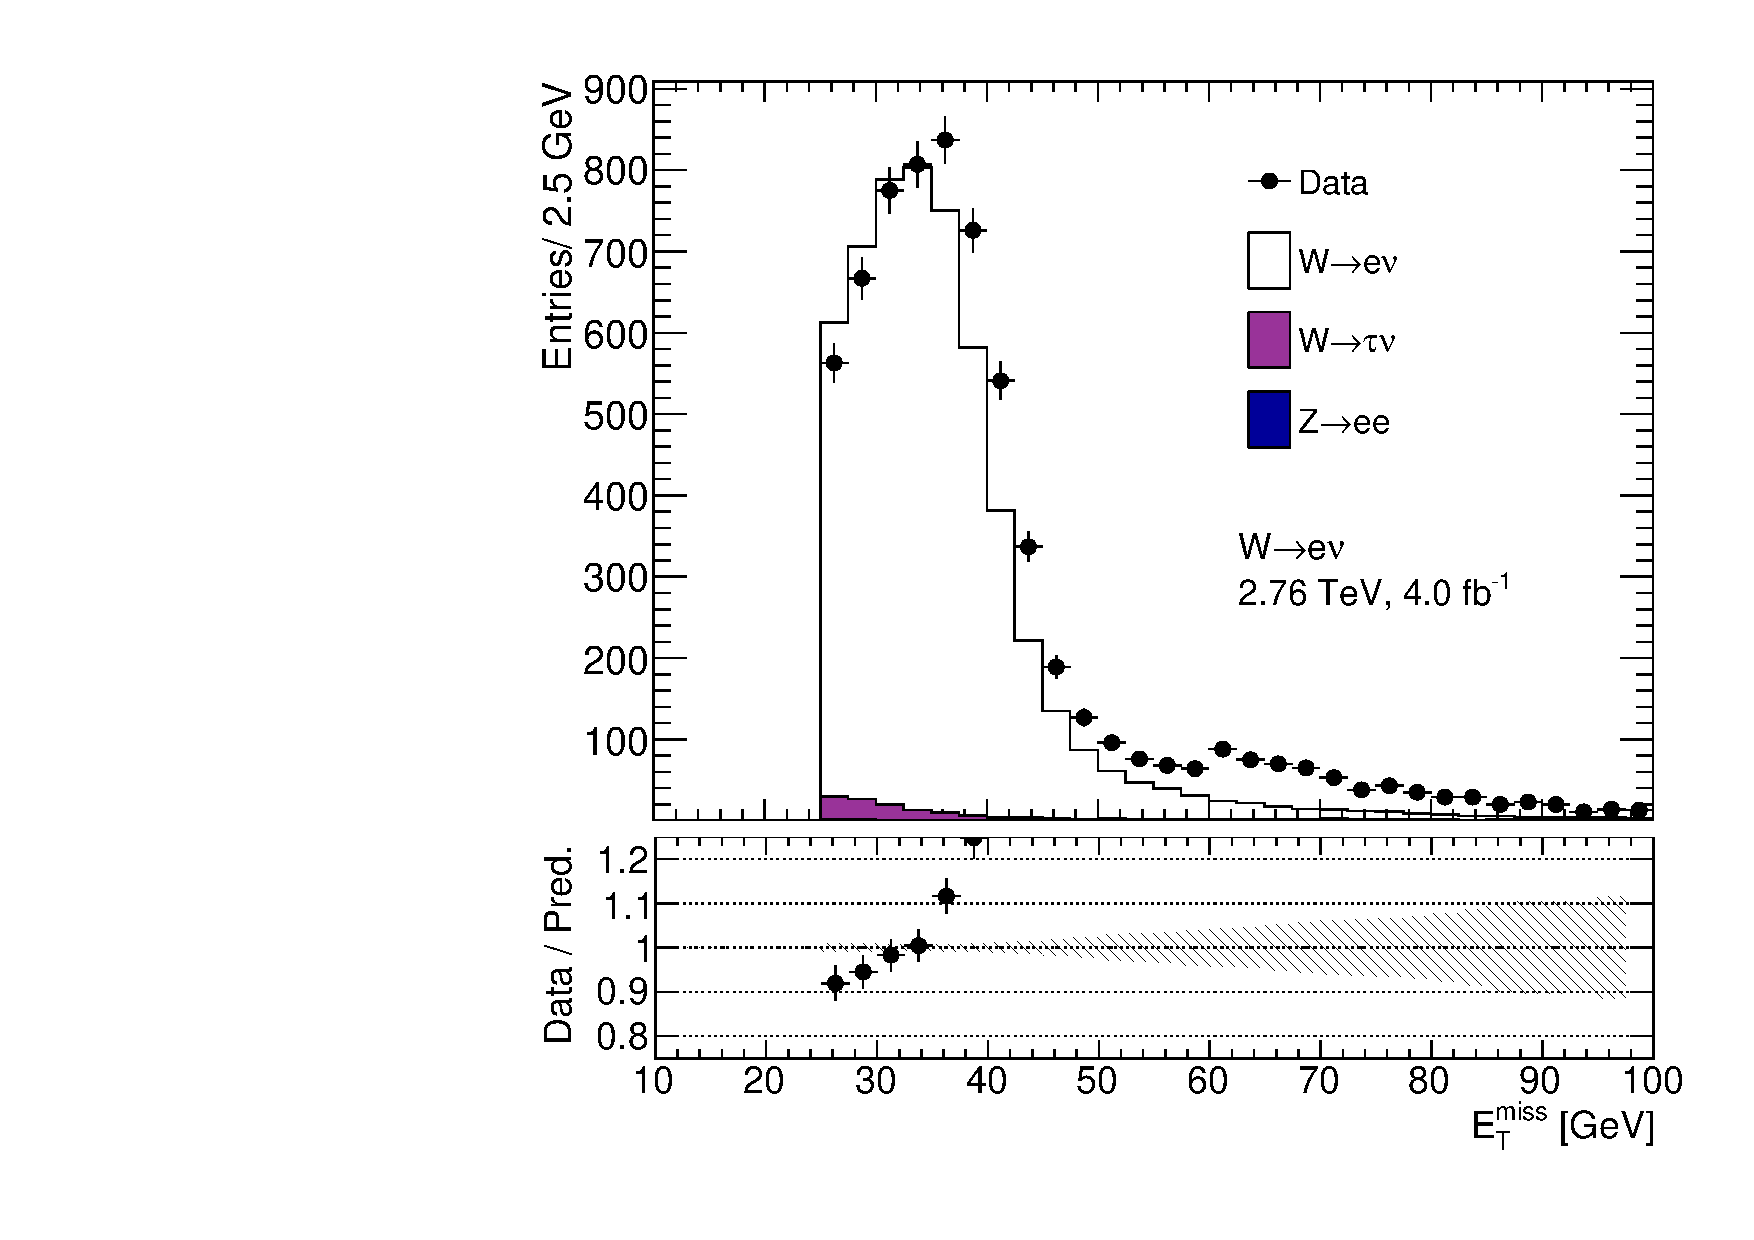
\includegraphics[width=1.\linewidth]{HadronRecoil/WenuRefFinal.pdf} \\ a)}
\end{minipage}
\hfill
\begin{minipage}[h]{0.49\linewidth}
\center{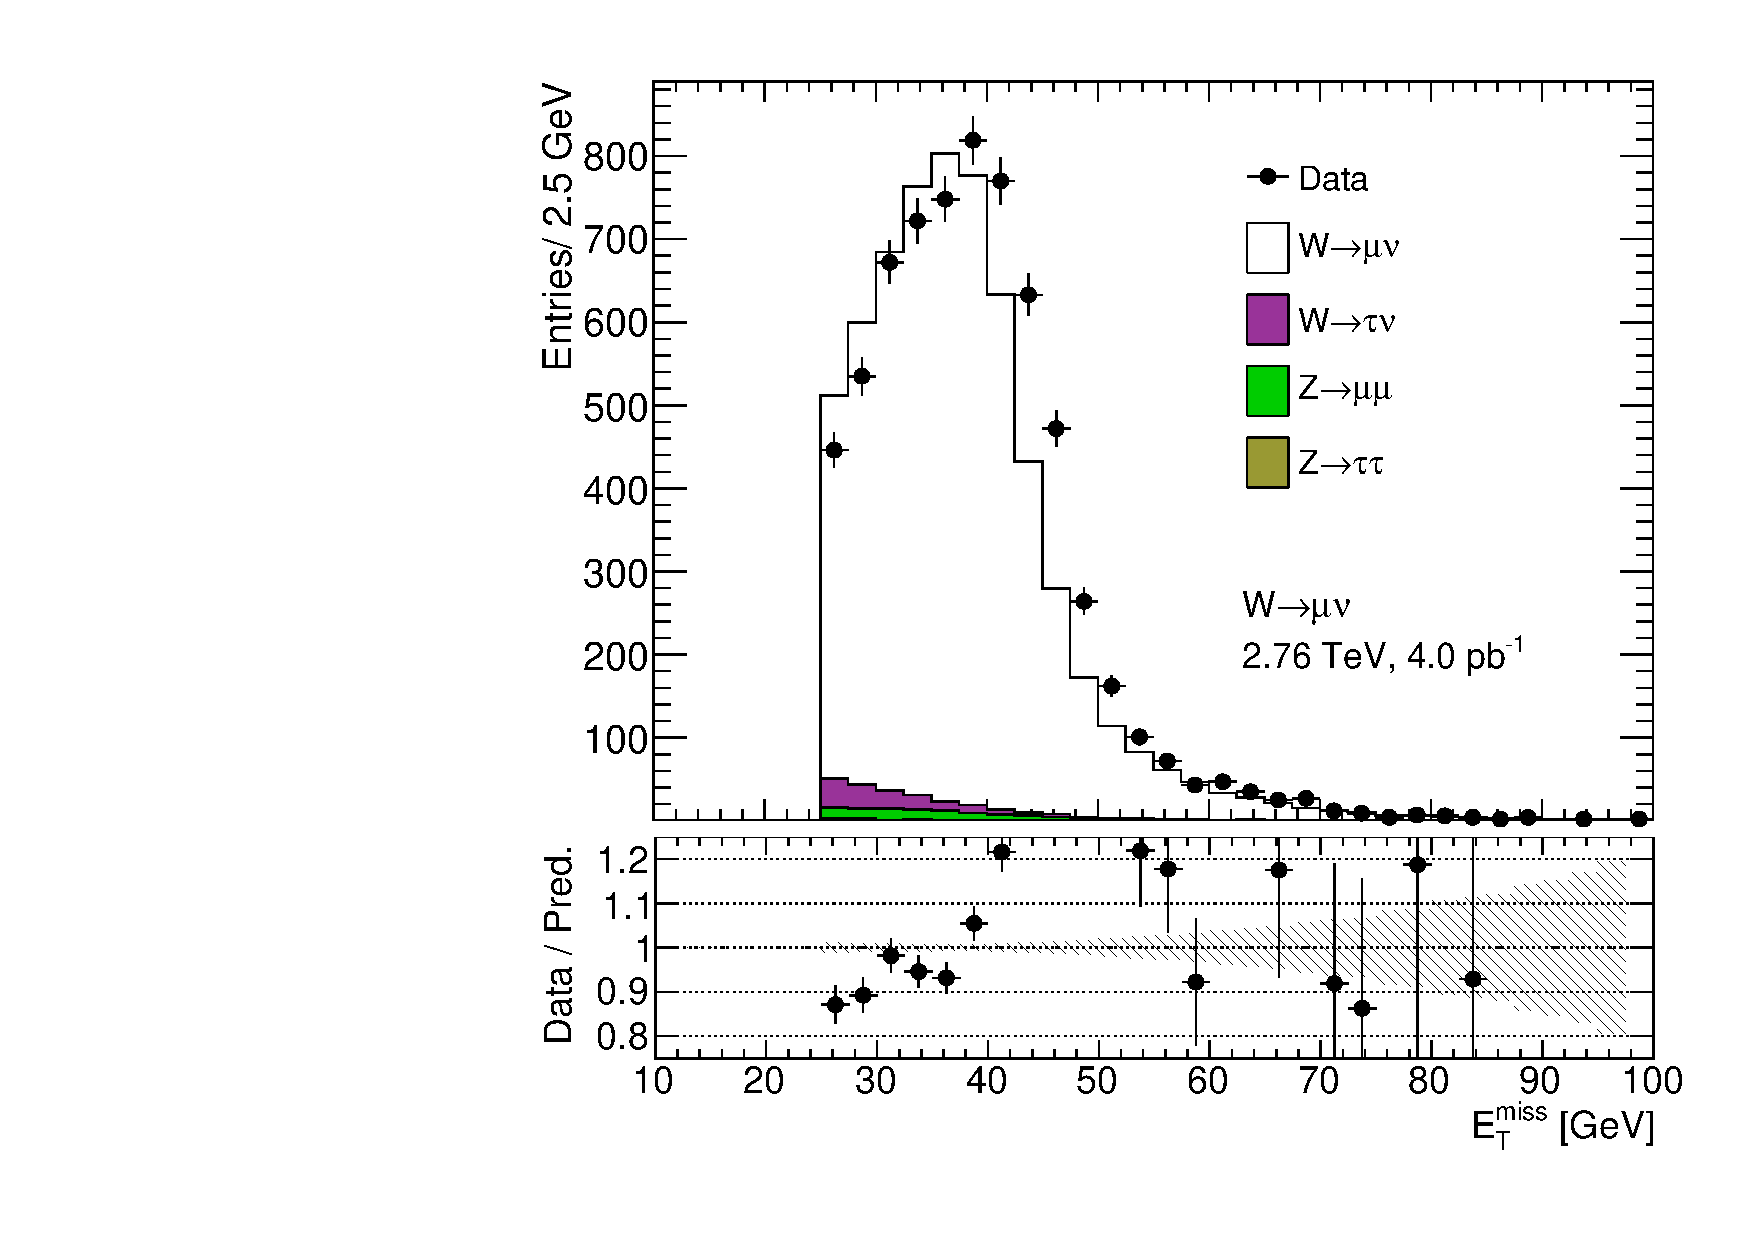
\includegraphics[width=1.\linewidth]{HadronRecoil/WmunuRefFinal.pdf} \\ b)}
\end{minipage}
\caption{Missing transverse energydistribution for a) the \wenu selection and  b) the \wmunu selection from Chap. \ref{chap:EventSelection}. \etmiss  calculated using the standard \atlas algorithm. The expected contributions from all backgrounds are estimated with Monte Carlo simulations, except for QCD background that is not included. All Monte-Carlo corrections from Chap. ~\ref{chap:MCCor} are applied. There are visible discrepancies between data and MC, that cannot be explained by the contribution of QCD background, which is expected mainly in the low \etmiss region (Sec. \ref{sec:QCD}).}
\label{ris:EtMissRefFinal}
\end{figure}

Standard reconstruction of \etmiss at \atlas experiment uses transverse energy deposits in the calorimeter, energy losses in cryostat and reconstructed muons for a calculation:
\begin{equation}
E_{x(y)}^{miss} = E_{x(y)}^{miss, calo} +  E_{x(y)}^{miss, cryo} +  E_{x(y)}^{miss, muon}.
\end{equation}
Calorimeter term is using information from reconstructed physics objects for calibration of cell responce. The total transverse energy in calorimeter is defined as:
\begin{equation}
E_{x(y)}^{miss} = E_{x(y)}^{miss, e} + E_{x(y)}^{miss \gamma} + E_{x(y)}^{miss, \tau} + E_{x(y)}^{miss, jets} + E_{x(y)}^{miss,SoftTerm} + E_{x(y)}^{miss, \mu}.
\end{equation}
where each term is calculated as a negative sum of the calibrated reconstructed objects, projected onto the x and y directions. Each jet with energy $P_T$>20 GeV is corrected for a pile-up and a jet energy scale is applied. Soft term is calculated from topoclusters and tracks, that are not assosiated with high-pt objects. To avoid double counting, muon energy loss  in the calorimeter is  subtracted from \etmiss.  The \etmiss muon term is calculated from the momenta of muons measured in a range of pseudorapidity. Since pileup has a significant effect on a \etmiss performance several methods of pileup suppression are used.

The runs at 2.76 TeV are characterized by a low pileup (mean number of interaction per bunch crossing < 1.0), so the usage of a procedure optimized for high pileup 8 TeV runs may not be optimal. It was examined and figured out, that there are big discrepancies between \etmiss distributions for data and MC simulation, as shown on a Fig. ~\ref{ris:EtMissRefFinal}, where the missing transverse energy for data is compared to signal and background MC predictions. 

The differences are visible in both electron and muon channels and cannot be explained by the (missing on the control plots) contributions from the QCD background, which is expected mainly in the low \etmiss region (see Sec. \ref{sec:QCD}). 



\subsection{Reconstruction of Missing Transverse Energy from hadron recoil}


\begin{figure}[!tbp]
\begin{center}
\begin{minipage}[h]{0.49\linewidth}
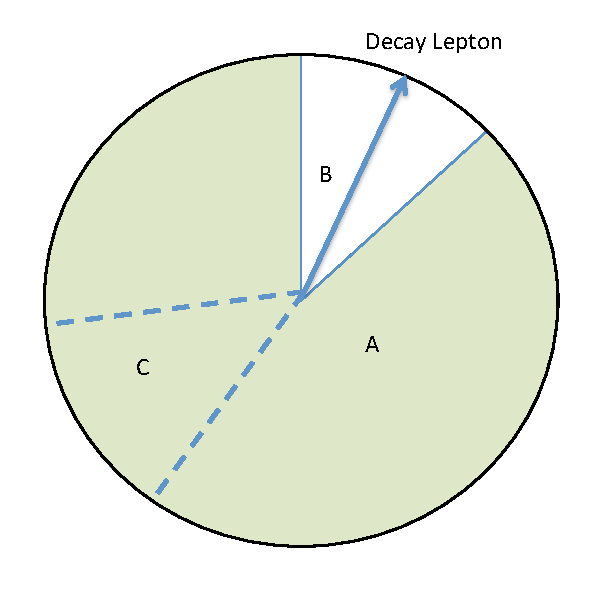
\includegraphics[width=1\textwidth]{HadronRecoil/ReplacementCluster.pdf}
\end{minipage}

\caption{Definition of different zones in the calculation of the cluster-based hadronic recoil. Zone B is excluded from hadron recoil calculation because it contains decay lepton. To describe properly overall acitivity it is replaced by the zone C, rotated in the direction of B. Zone A corresponds to the rest of the calorimeter.}
\label{ris:subsCone}
\end{center}
\end{figure}

Different way of \etmiss calculation  was developed for W and Z decays by W mass measurements group \cite{FirstHR}. This procedure based on the requirement of balance in transverse momentum of a W-boson and the initial (quark-gluon) state radiation,:
\begin{equation}
\vec{P}_{T}^{W} = \vec{P}_T^l+\vec{P}_T^{\nu}= \sum{\vec{P}_{T}^{ISRquarks,gluon}}, 
\end{equation}
where $\sum{\vec{P}_{T}^{ISRquarks,gluon}}$ is a transverse momentum of partons from initial state radiation, also called hadronic recoil (HR). Therefore, \etmiss can be determined as:
\begin{equation}
E_{T}^{miss} = P_T^{\nu} =  - HR + p_T^{l}
\end{equation} 

This procedure assumes, that recoil is arises from one single leading jet, and the rest  is coming from a soft hadronic activity. This hadron recoil is computed as a vector sum of calorimeter clusters:
\begin{equation}
HR= \sum_{i=0}^{N_{topo}}\vec{p_T^{topo}}
\end{equation}
while a scalar sum of all transverse energies is corresponding to the hadronic activity of the event:
\begin{equation}\label{eq:sumet}
\sum E_T =\sum_{i=0}^{N_{topo}} E_T^{topo}
\end{equation}
To avoid double counting of lepton energy losses in calorimeter, the clusters inside cone with radius dR = 0.2 are excluded from this calculation.To compensate soft activity inside this cone, clusters are then compensated by replacement cone (Fig. \ref{ris:subsCone}). This cone is defined as cone at the same pesudorapidity, but different $\phi$. It should be far from any other lepton and hadron recoil direction. Each cone is then rotated to a direction of the original lepton direction. This definition is not taking into account jet reconstruction aspects.   This is allowing to get a better data MC agreement (Fig. \ref{ris:HadrRecoilEtMiss}).


\begin{figure}[!tbp]
\begin{minipage}[h]{0.49\linewidth}
\center{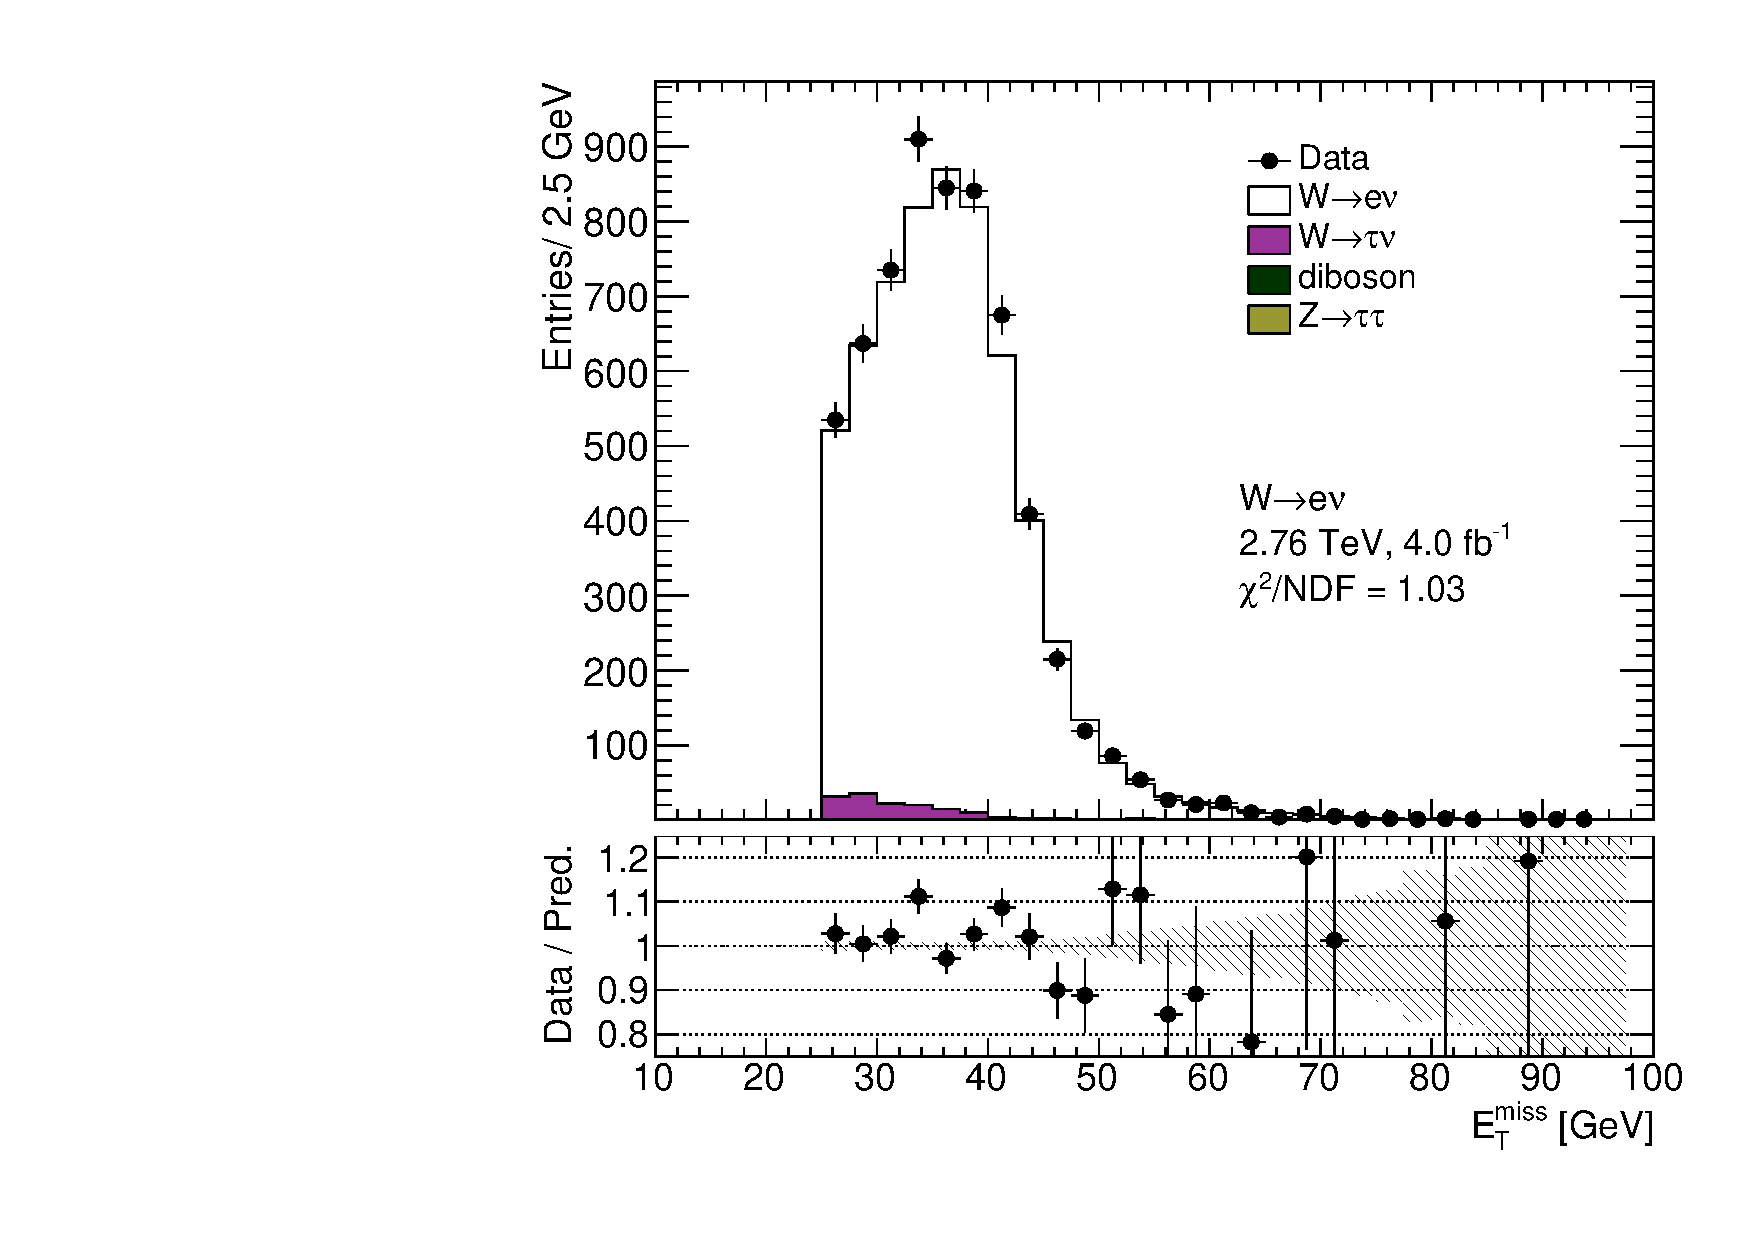
\includegraphics[width=1.\linewidth]{HadronRecoil/W_Boson_etMiss.pdf} \\ a)}
\end{minipage}
\hfill
\begin{minipage}[h]{0.49\linewidth}
\center{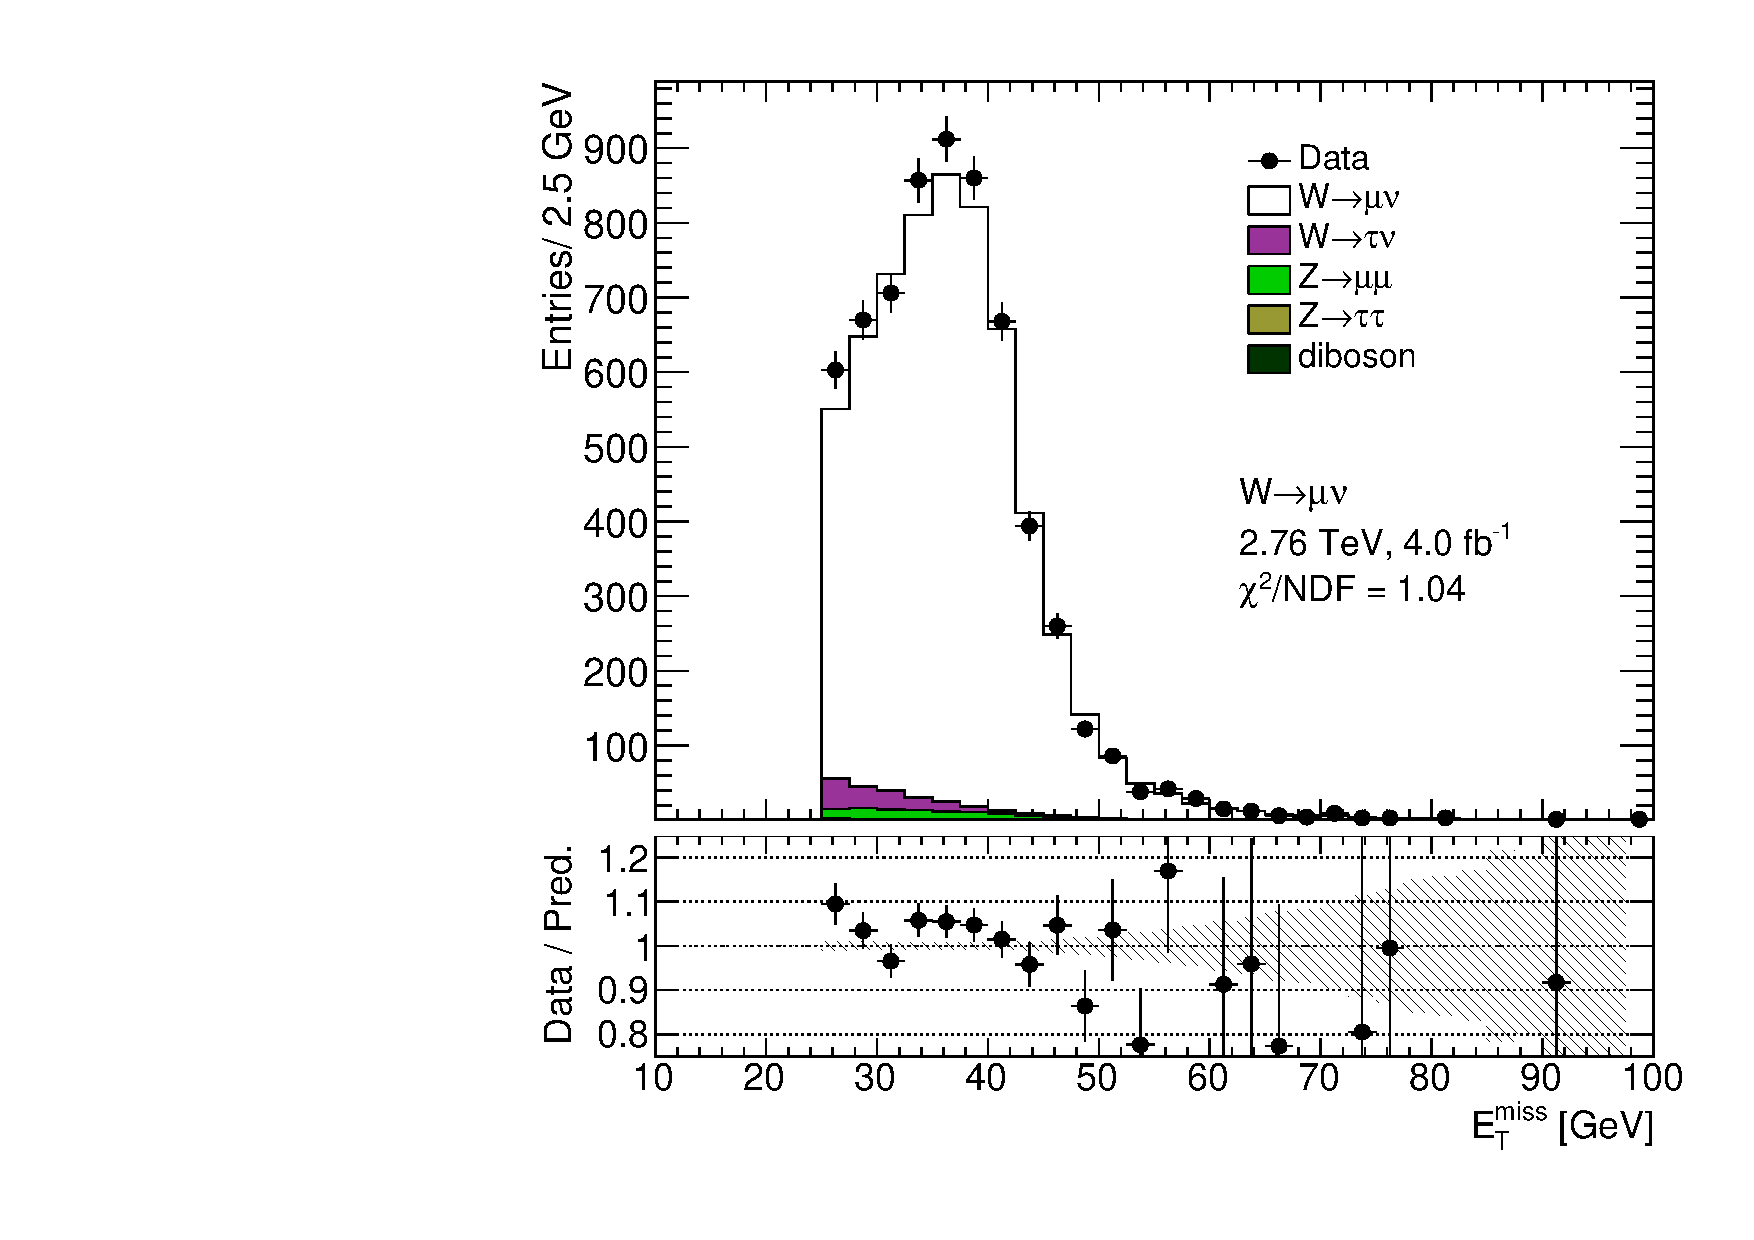
\includegraphics[width=1.\linewidth]{HadronRecoil/Wmu_Boson_etMiss.pdf} \\ b)}
\end{minipage}
\caption{Data and MC comparison for \etmiss calculated from hadron recoil for a)\wenu b)\wmunu events}
\label{ris:HadrRecoilEtMiss}
\end{figure}



  
\chapter{Monte Carlo}\label{chap:MC}
The Monte Carlo(MC) method was invented by scientists working on the atomic bomb in the 1940s. Its core idea is to use random samples of parameters or inputs to explore the behavior of a complex system or process.  Nowadays, MC are essential part of both theoretical and experimental particle physics research.
This chapter gives an overview of ATLAS experiment simulation scheme, simulation methods and software used. Also, a techniques for fast simulation will be discussed. 

\section{Monte Carlo simulation at ATLAS experiment}

\begin{figure}[h]
\center{
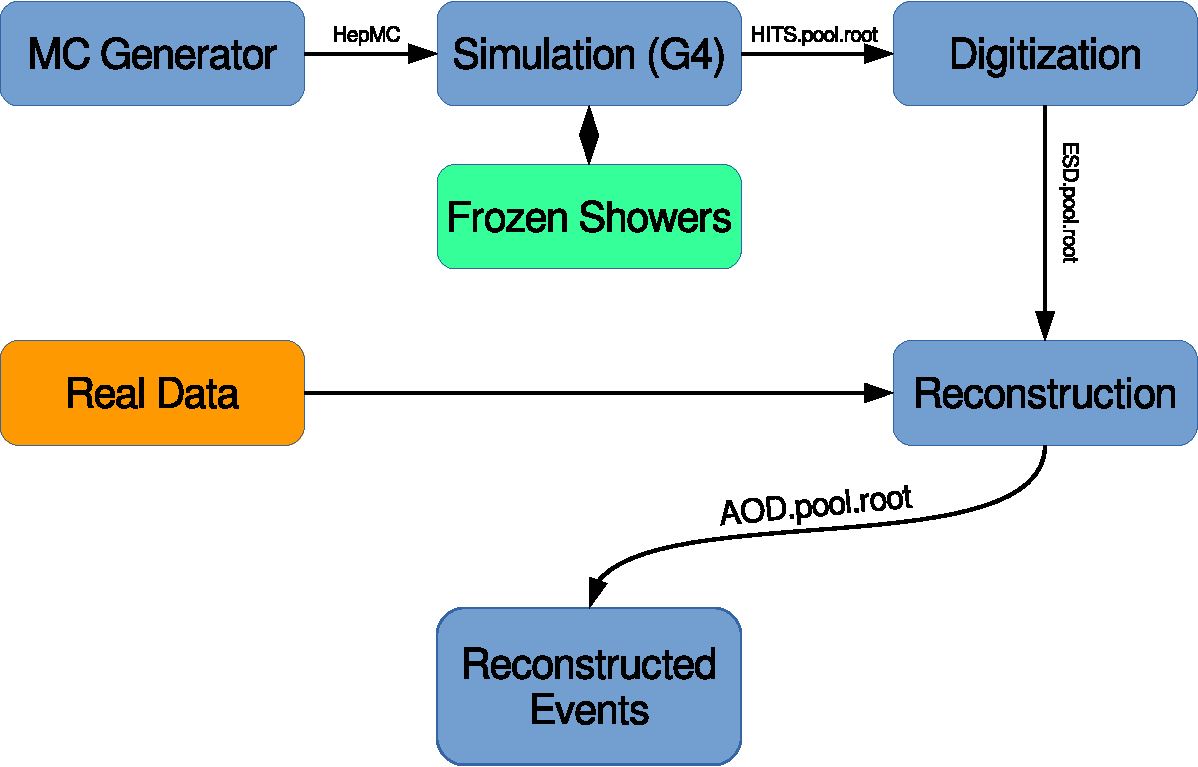
\includegraphics[width=0.6\textwidth]{MC/MC_production_chain2.pdf}
\caption{Diagram of the ATLAS MC production chain}
\label{fig:MC_gen}}
\end{figure}

MC is allowing to make different analysis, such as compare data with predictions, study detector or selection algorithms performance. All of this applications are requiring MC precision. Simulation software expects to use precise physics models for sampling and have large enough statistics, to exclude statistical uncertainties (usually 5 times more, than expected in a data). ATLAS simulation software is integrated into Athena and usually used during large production of events. Simulation chain is generally divided into 4 main steps (Figure ~\ref{fig:MC_gen}):
\begin{description}
\item[Event generation]Simulation of hard interaction and a resulting high-energy particles parameters. This step is independent of ATLAS detector geometry.
\item[Simulation]Simulation of energy depositions ("hits") done by final state particles in ATLAS detector.
\item[Digitalization] Simulation of detector responce using "hits" information:  first, inputs to the read out drivers (ROD's), called "digits" are constructed, then, ROD functionality is emulated. Detector noise effects are added at this stage. 
\item[Reconstruction] Production of the Analysis Object Data (AOD) files, which are containing sufficient information for physics analysis. This stage is identical for both data and MC
\end{description}
This is scheme allows to use computing resources more efficiently, than with a single-step simulation, and simplifies software validation, since it is possible to reuse files from previous stages. In the following sections event generation and simulation will be described in more details

\subsection{Event generators}

\begin{figure}[h]
\begin{center}
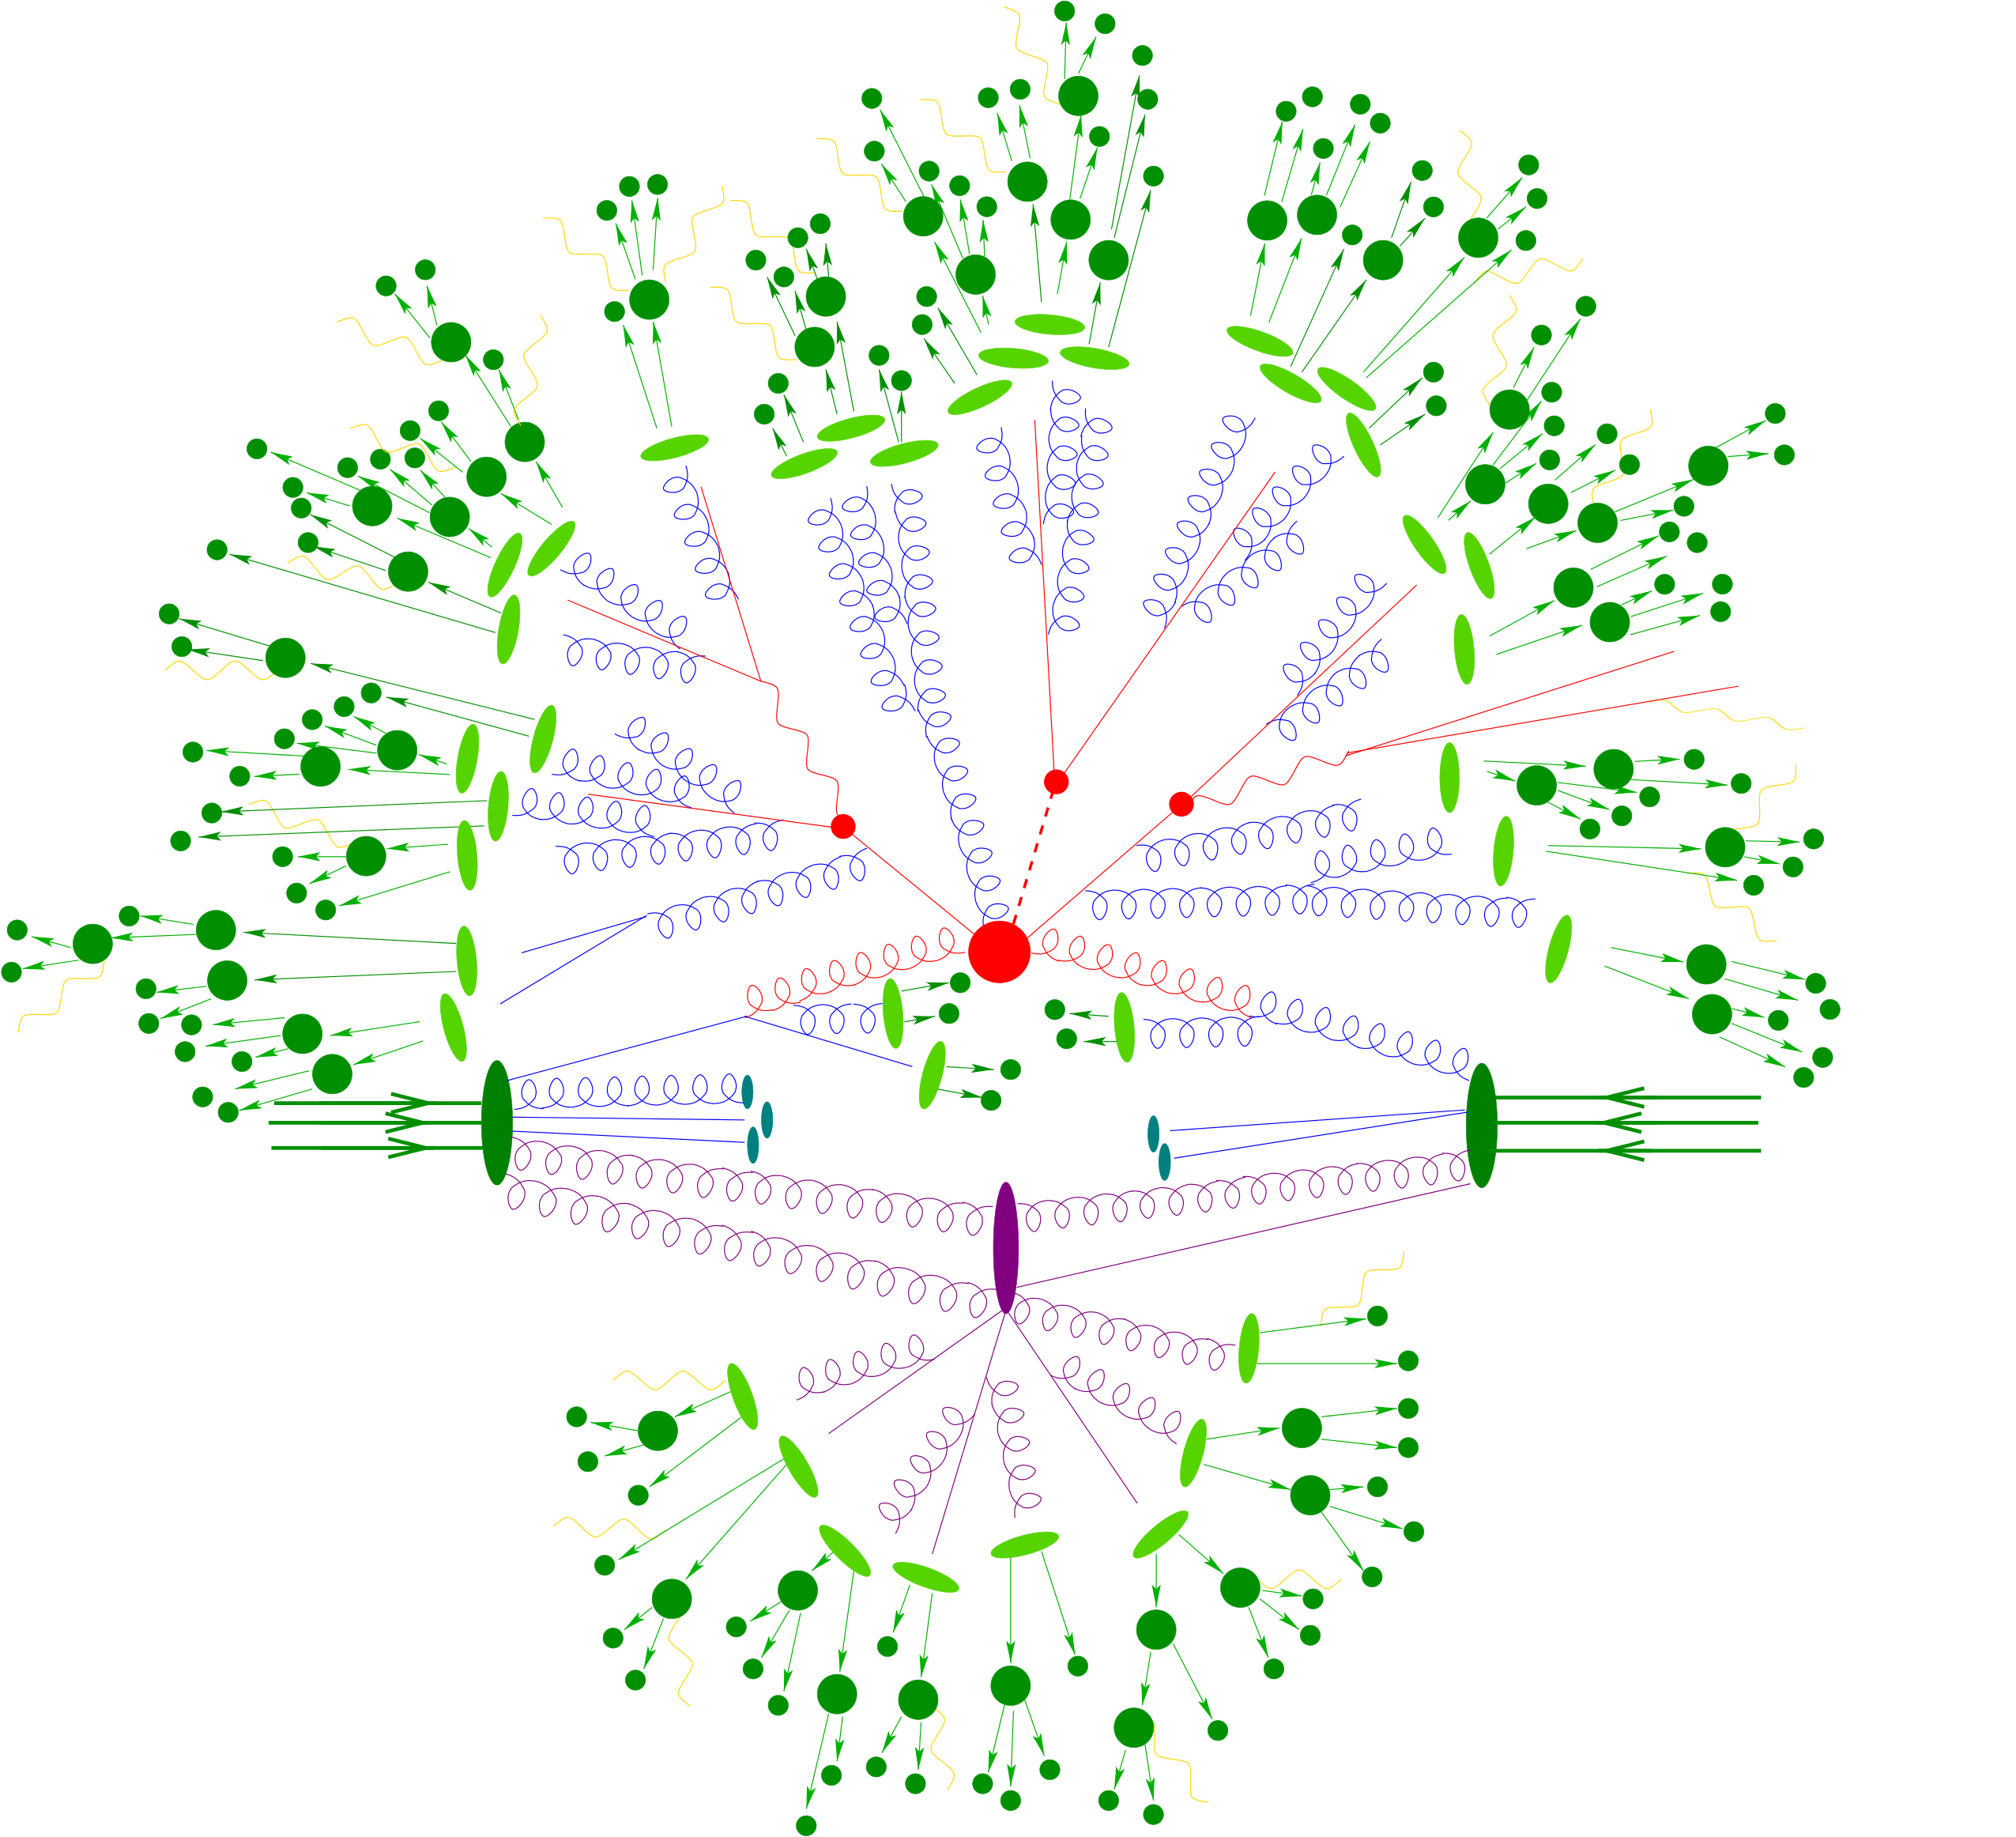
\includegraphics[width=0.5\textwidth]{MC/tth_Event}
\end{center}
\caption{Schematic view of a $t\bar{t}H$ event produced in a pp-collision: the hard scattering is shown as a red blob with the solid and dashed lines as the resulting three particles.
Independently happening multi-particle interactions are indicated by the violet blob. 
Parton showers are shown with curly lines.
Hadronization yields hadrons as shown in light green, while the final state particle are dark green.
}
\end{figure}

The outcome of the hard interaction could be simple scattering of the hadron elementary constituents, their annihilation into new resonances or a combination of two. In any case, the final state has a large particles multiplicity. The main goal of event generator is to provide a complete picture of this final states: description of the particle types and momentia on event-by-event basis. The factorisation theorem \cite{Factorisation} allows to make event generation in independent stages, which are dominated by different dynamics:
\begin{description}

\item[Modelling of hard subprocess] Hard subprocess is happening at the smallest scales of times and distance, where all of the colliding partons are considered free. Process of interest is simulated by selecting production channels and calculating corresponding matrix elements (ME) in the desired level of accuracy in pertrubation theory . Most of the generators have leading order or next to leading order ME in $\alpha_s$. 
\item[Parton showering] Quarks and gluons from hard process can radiate secondary quarks and gluons, resulting on the dozens of additional partons associated with the event. This process calculated as step-by-step evolution of momentum transfer scales from highest (hard subprocess), to the lowest (around 1 GeV). 
There is a possiblity of double counting between showers and hard subprocess. This can be avoided using matching approach, for which higher order corrections to ME are integrated with parton showers, or merging strategy, there jet resolution scale is used as an threshold between matrix elements and parton showers. 
\item[Hadronisation] Final stable color-neutral particles, what can be detected in experiment, are formed during hadronisation. This occures at larger nonpertrubative scales and  usually implemented using different phenomenological models.
\item[Modelling underlying event] Parallel to the main process other collisions of partons can occur, called underlying event. These additional interaction can produce partons which contribute to the final state. This is one of the least understood aspect of hadronic collisions. 

\end{description}

Schematic plan of simulation of ttbar event is shown in Figure \ref{fig:MC_ttH}. The hard scattering itself is shown as a red blob with the solid and dashed lines indicating the resulting particles, which themselves decay further. 
Underlying event is indicated by the violet blob. 
Parton showers are shown with curly lines.
Hadronization yields hadrons as shown in light green, while the final state particles are dark green.

The current analysis uses samples generated with the following generators:
\begin{itemize}[align=left]
\item[Powheg \cite{Powheg}] Powheg is generator with NLO ME \cite{PowhegNLO}, that can be interfaced with other generator(such as Pythia or Herwig) for higher precision of showering.
\item[Pythia \cite{Pythia6}] Pythia is a general purpose generator for hadronic, hadron-lepton and leptonic collisions. It can model initial and final state showers, hadronisation and decays, underlying event (via multi parton interactions). Pythia contains library with around 240 processes with LO ME. It uses Lund String model \cite{LundString} for hadronisation.
\item[Herwig \cite{Herwig}] Herwig is a LO general purpose event generator for simulation lepton-lepton, hadron-lepton and hadron-hadron collisitons. The main difference between Pythia and Herwig is that it is uses angular ordering in the parton showers and also models the hadronisation step based on the cluster fragmentation
\item[Sherpa \cite{Sherpa}] Sherpa is a generator with tree level of matrix elements, featuring its own implementation of parton shower and hadronisation models.
\item[Photos \cite{Photos}] Precision tool for QED radiative corrections in W and Z decays.
\item[Tauola \cite{taluola}] Generator, used to describe leptonic ans semi-leptonic $\tau$-decays.
\end{itemize}

\subsection{Simulation in Geant4}

After event generation, simulation software obtains hardware response for final state particles. The main method used by ATLAS, referred to as \textit{Full Simulation}, makes use of the Geant4\cite{Geant4}. It is C++ based toolkit for the simulation of the passage of particles through matter. It is used in a wide range of experiments in high energy and nuclear physics.

Geant4 can simulate complex detector structures with sensitive detector material and corresponding infrastructure. It can also calculate basic properties of materials, like radiation and interaction length. For detector Geant4 stores "hits" information  - snapshots of physical interactions. 
In Geant4 events and particles are simulated separately and each particle is moved step by step. Size of this step is chosen to preserve both CPU performance and required precision. Physics is treated as a set of discrete processes. They could be handled either at rest, along step or after it. Geant4 package has different models and approximations for hadronic and electromagnetic processes. Some of them are not approximate, but computationally fast. It allows to choose set of the models, called physics list, depending on particular requirements. There are several reference physics lists, that are validated for each new release of Geant4 software. \atlas experiment is using one of this lists.

It is necessary to have mass MC production for each data taking, what is taking most of the resources. Uncertainties of some of Run-I analyses are dominated by available MC statistics. 

It is possible to improve in CPU usage by tuning physics list or working on a magnetic field parametrisation. Also there are long term developments for multi-threading and vectorisation of the code. 
Yet, Run-2 has a higher pileup and luminosity, so even more MC events are needed. This means that fast and accurate simulation approach is essential. During simulation largest time is spend on calorimeters. This is the motivation for development of fast calorimetry techniques.  

There are two main methods used in ATLAS:
\begin{itemize}
\item Parametrisation of calorimeter cells responce. Spacial energy responce is simulated using longitudial and lateral energy profiles.
\item Frozen Showers. This technique will be described more detailed in the following section
\end{itemize}


\subsection{Frozen Showers}
Main principle of this method is described by its name. It is using pre-simulated "frozen" showers generated in full simulation and stored in a library. Particles below minimum energy
thresholds are killed and replaced with with these showers. All of the other particles are simulated using full simulation. This process is schematically shown in a Figure ~\ref{fig:MC_FS_method}.
\begin{figure}[t]
\center{
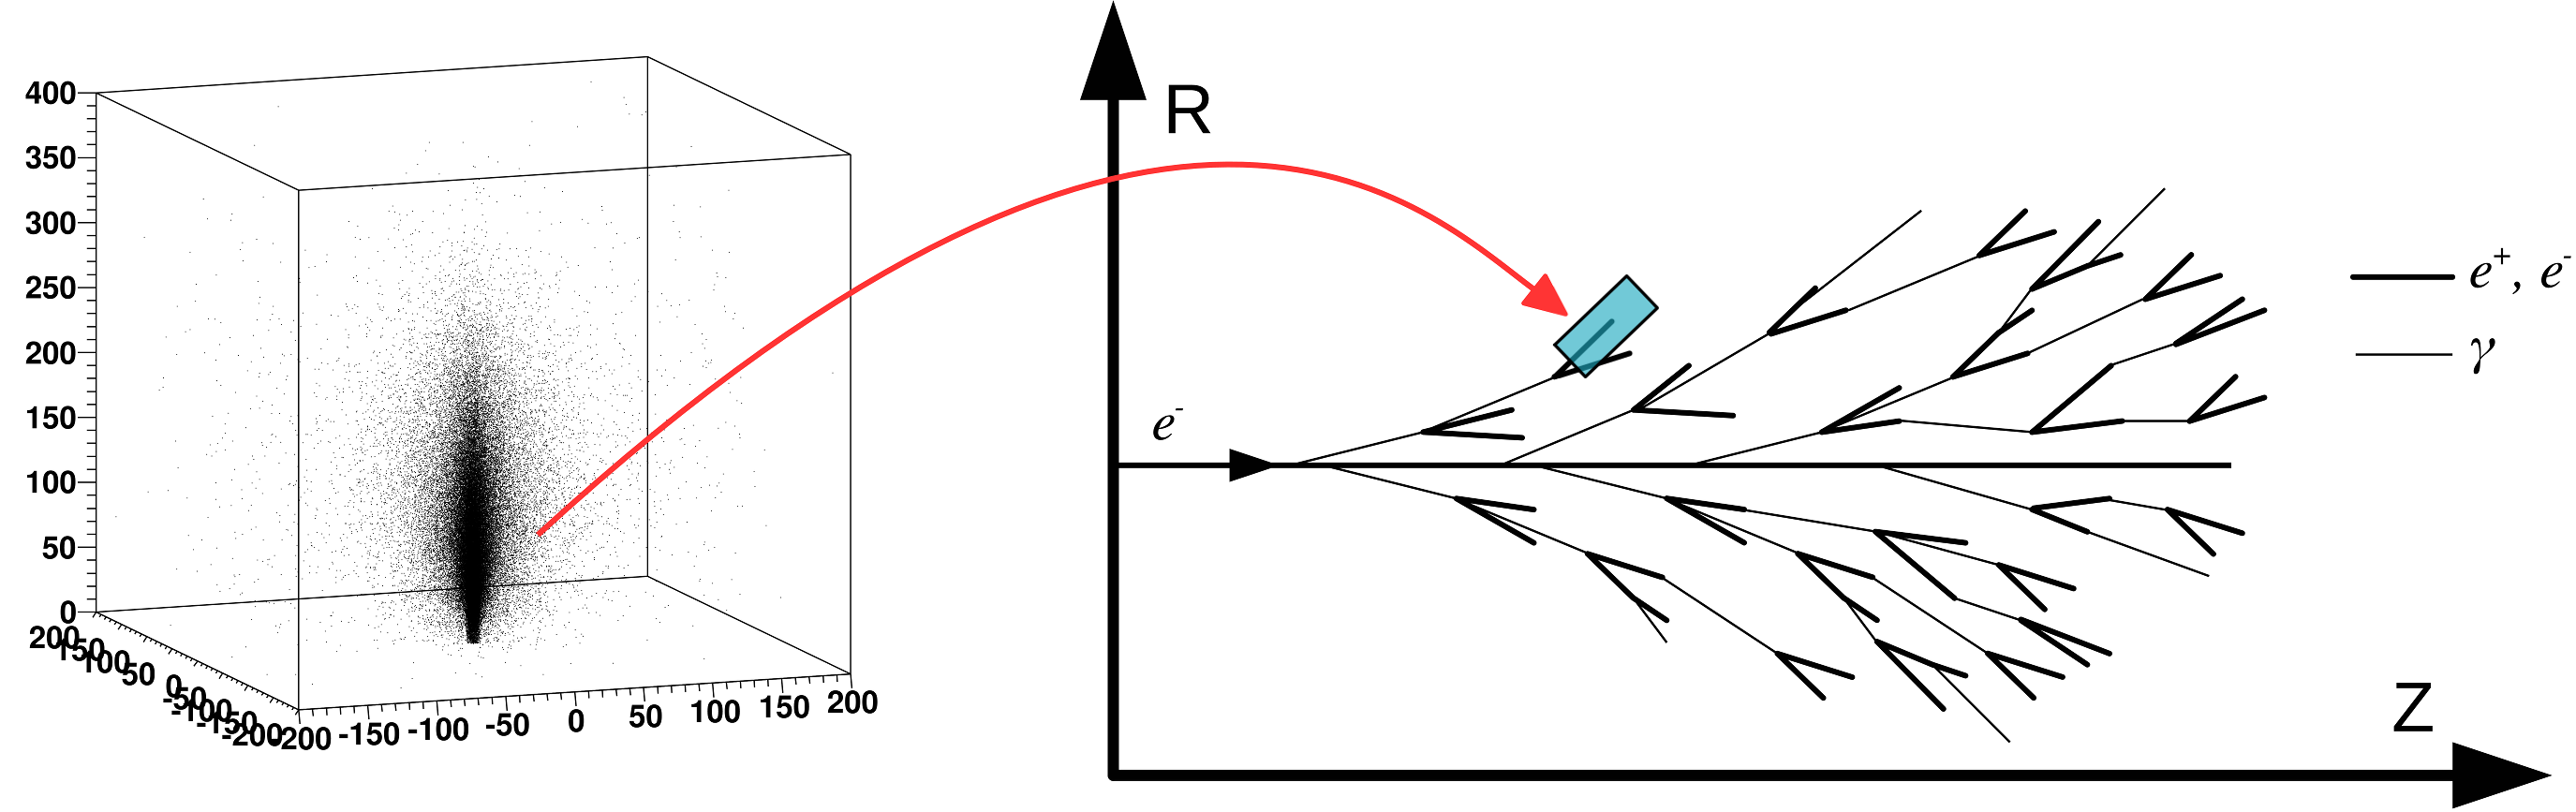
\includegraphics[width=1.0\textwidth]{MC/MC_FS_method.png}
\caption{Diagram showing the shower substitution of the low-energy particle, during the high-energy particle simulation.}
\label{fig:MC_FS_method}}
\end{figure}

The library itself organized as follows: the header contains basic simulation parameters, like Geant4, geometry and \atlas software release version and physics list used. Showers are stored in a bins of positional  variables (see sec. \ref{sec:FSProd}), while energy remain unbinned. Each shower stores lateral and transverse size and information about energy, time and positions of the hits.

\subsubsection{Production use of Frozen Showers}\label{sec:FSProd}

\begin{figure}[t]
\center{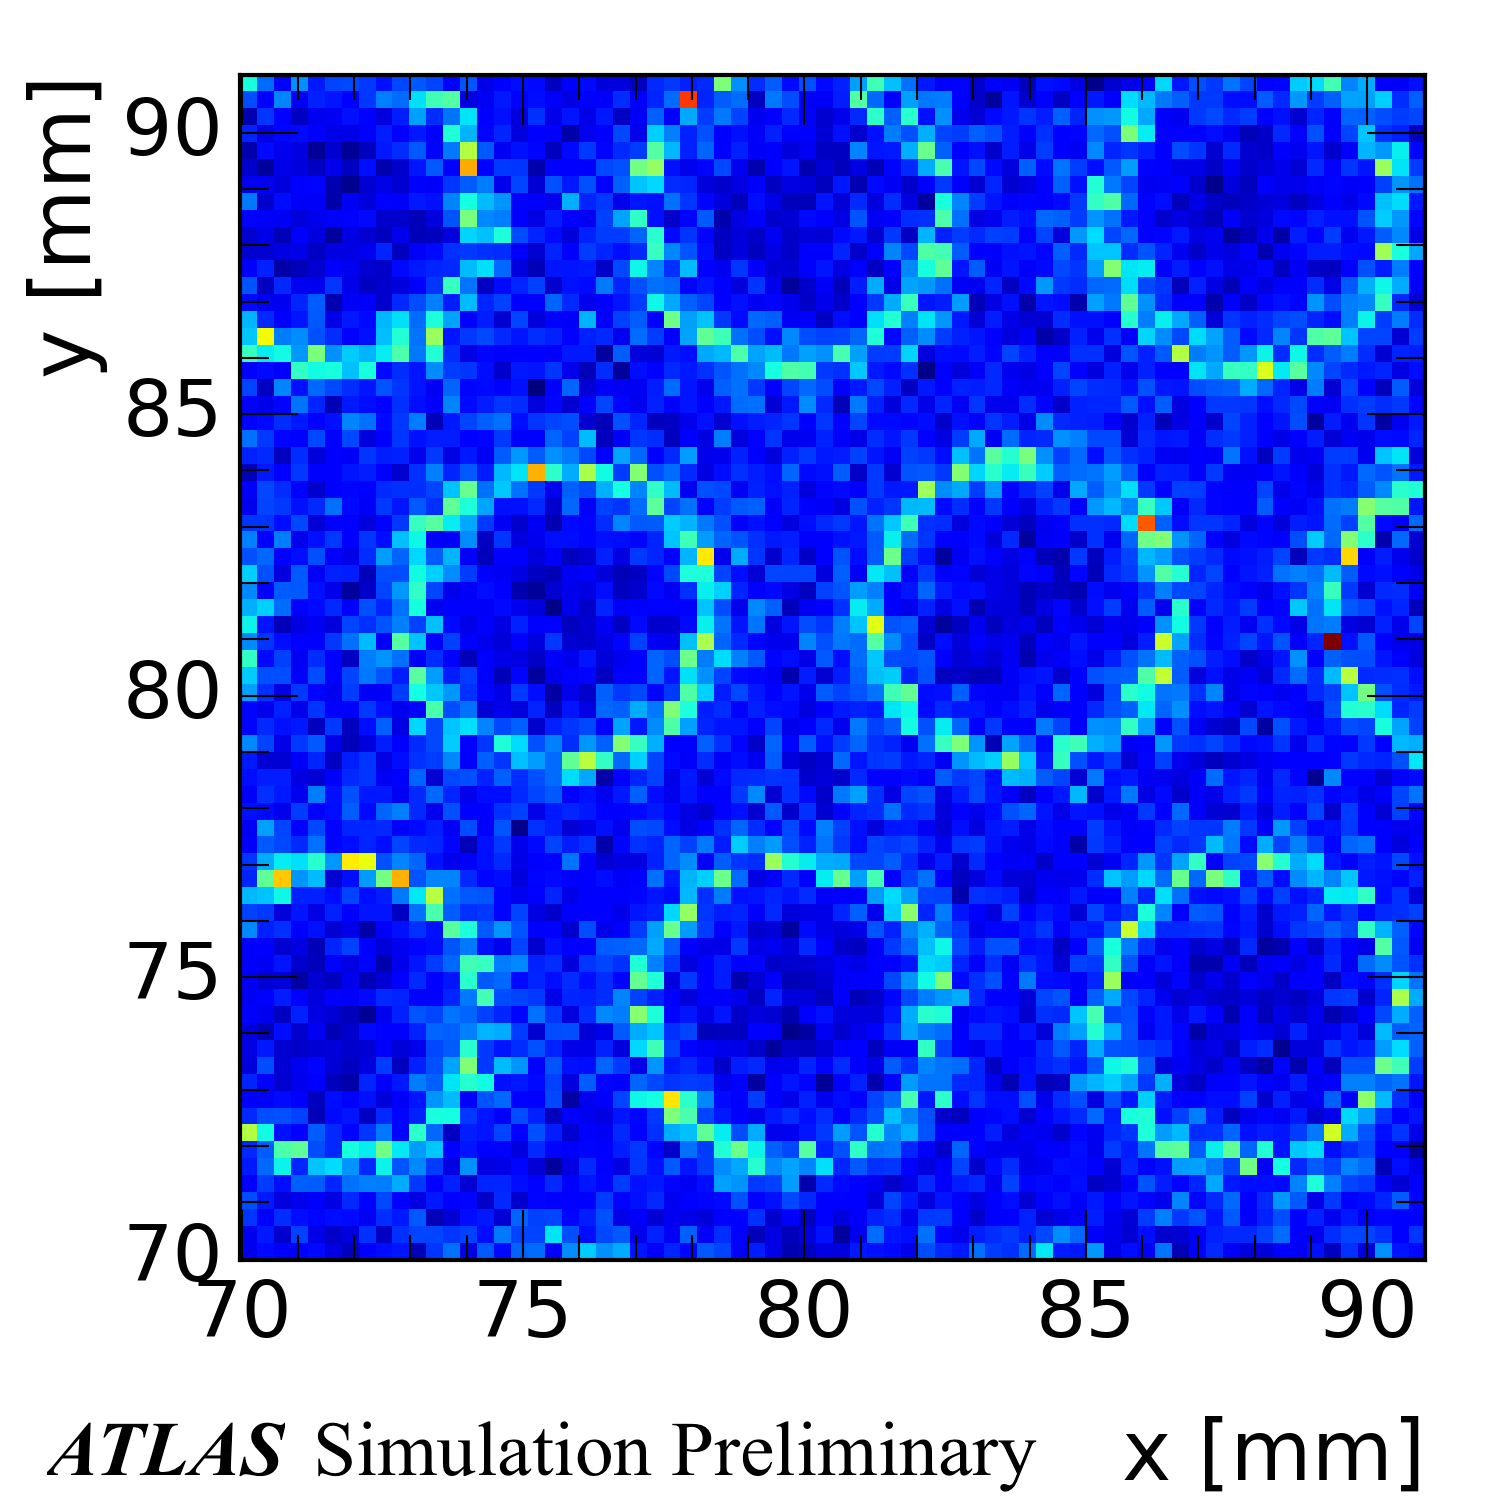
\includegraphics[width=0.5\linewidth]{MC/xySumE.png} }
\caption{Average energy response in a calorimeter vs x,y for electrons with energy less than 1 GeV }
\label{fig:FSFluctuations}
\end{figure}


\begin{figure}[t]
\center{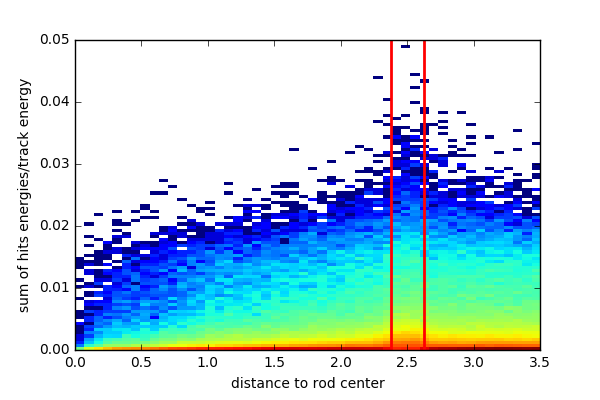
\includegraphics[width=1.\linewidth]{MC/fullBinningScatter.png} }
\caption{Energy response for electrons in a calorimeter for all electrons in a library}
\label{fig:FSProduction}
\end{figure}

\begin{figure}[t]
\begin{minipage}[h]{0.49\linewidth}
\center{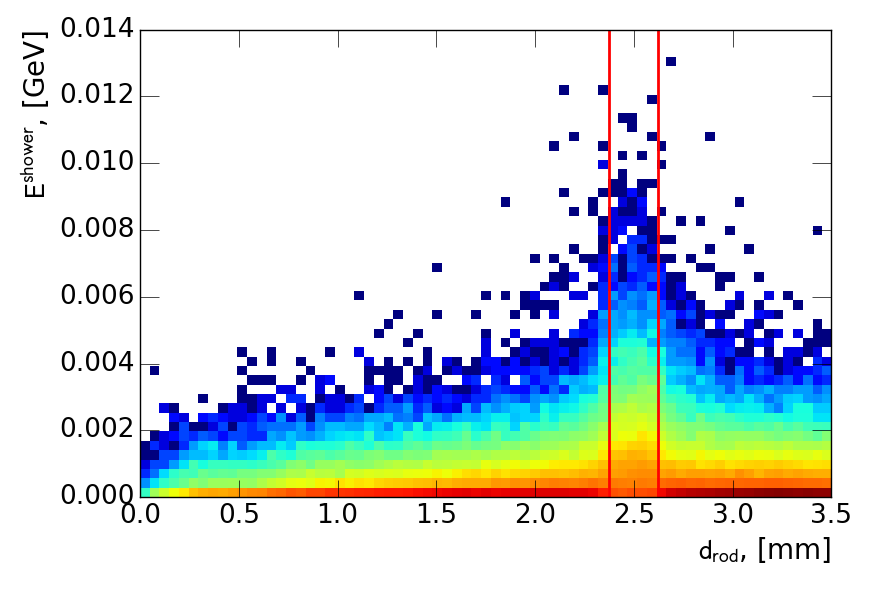
\includegraphics[width=1.\linewidth]{MC/fullBinningScatterSmall.png} \\ a)}
\end{minipage}
\hfill
\begin{minipage}[h]{0.49\linewidth}
\center{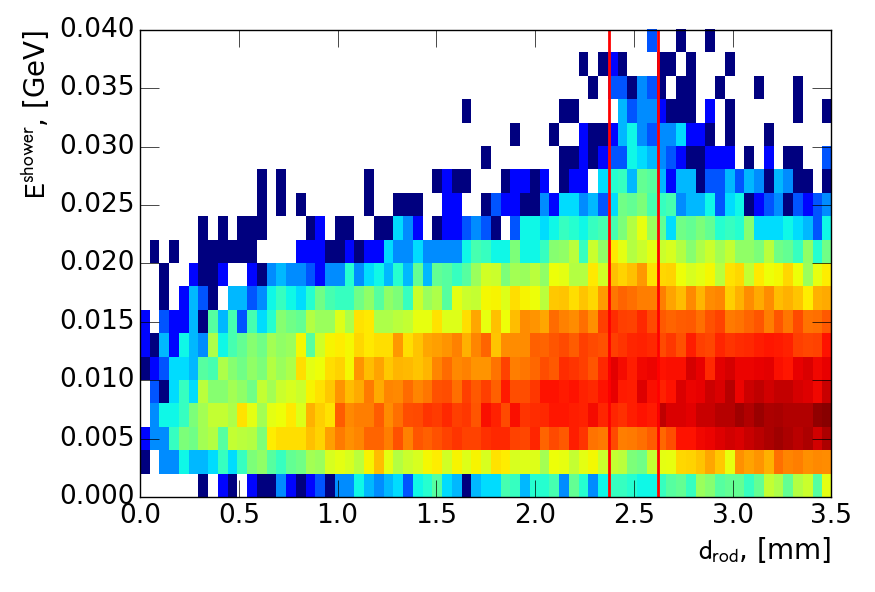
\includegraphics[width=1.\linewidth]{MC/fullBinningScatterBig.png} \\ b)}
\end{minipage}
\caption{Energy response for electrons in a calorimeter for  a) electrons with energy less than 100 MeV b) electrons with energy bigger, than 100 MeV}
\label{fig:FSProduction2}
\end{figure}


During simulation, if an energy of a particle falls below cut-off energy, the particle algorithm examines resulting shower containment. It checks  that particle is far from the edges of calorimeter, so what shower will be by 90\% inside calorimeter. This dependes also on a energy of particle, because shower sizes are growing with energy.
When particle is removed and substituted by shower taken from corresponding eta and distance bin with the closest energy found. Energies of the hits in shower found are scaled to fully correspond to particle energy. Additionally, shower direction is changed to the direction of the particle.

Frozen Showers have been used in \atlas Monte-Carlo production since run-1. This method is applicable for all LAr calorimeters in \atlas, but currently it is enabled for simulation of forward calorimeters (FCAL), since it is showing the smallest differences, compared to the other fast simulation methods (e.g parametrisation). This is because of large of non-uniformly distributed sensitive material, which is giving different responce, than a dead material (Figure ~\ref{fig:FSProduction}). Resolution of a calorimeter can be written as:
\begin{equation}\label{eq:EMResoultion}
\frac{\sigma}{E} \approx \frac{1}{\sqrt{E}}	\oplus \frac{1}{E} 	\oplus const,
\end{equation}
where symbol $\oplus$ indicates a quadratic sum. The first term is 'stocastic term', which includes intrinsic shower fluctuations, second takes into account readout noise effects and pile-up fluctuations. Constant term derives from non-uniformities in a detector, what are causing large fluctuation of the energy loss. Resolution of high-energy electrons is mostly dominated by this term. Example of these fluctuations is shown on a Figure ~\ref{fig:FSFluctuations}. Cirles are corresponding to a LAr gaps inside FCAL. It can be seen, that particles inside sensitive material are having more energetic showers, than particles in a dead material. It is possible to capture this structure by introducing  distance to a closest rod center:
\begin{equation}
D = min(\sqrt{dx^2+dy^2}, \sqrt{(step_x-dx)^2+dy^2}, \sqrt{(step_x/2-dx)^2-(step_y-dy)^2}), 
\end{equation}
where dx and dy are the distances to a rod center in a x and y plane respectivelly. They are calculated as:
\begin{equation}
dy = y-n[]
\end{equation}

Dependency of summed energy of shower on the distance defined above is shown on a Figure ~\ref{fig:FSProduction}. Gap is marked by the red lines. Size of this differences between sensitive material and dead material depends on a initial particle momentia (Figure ~\ref{fig:FSProduction2} a and b). For electrons with energy greater than 500 GeV they are almost negligible. Additionally, at higher energies gain in a CPU time is moderade, while library becomes bigger. This is reason for an upper limit to be set at 1000 MeV
\begin{figure}
\center{
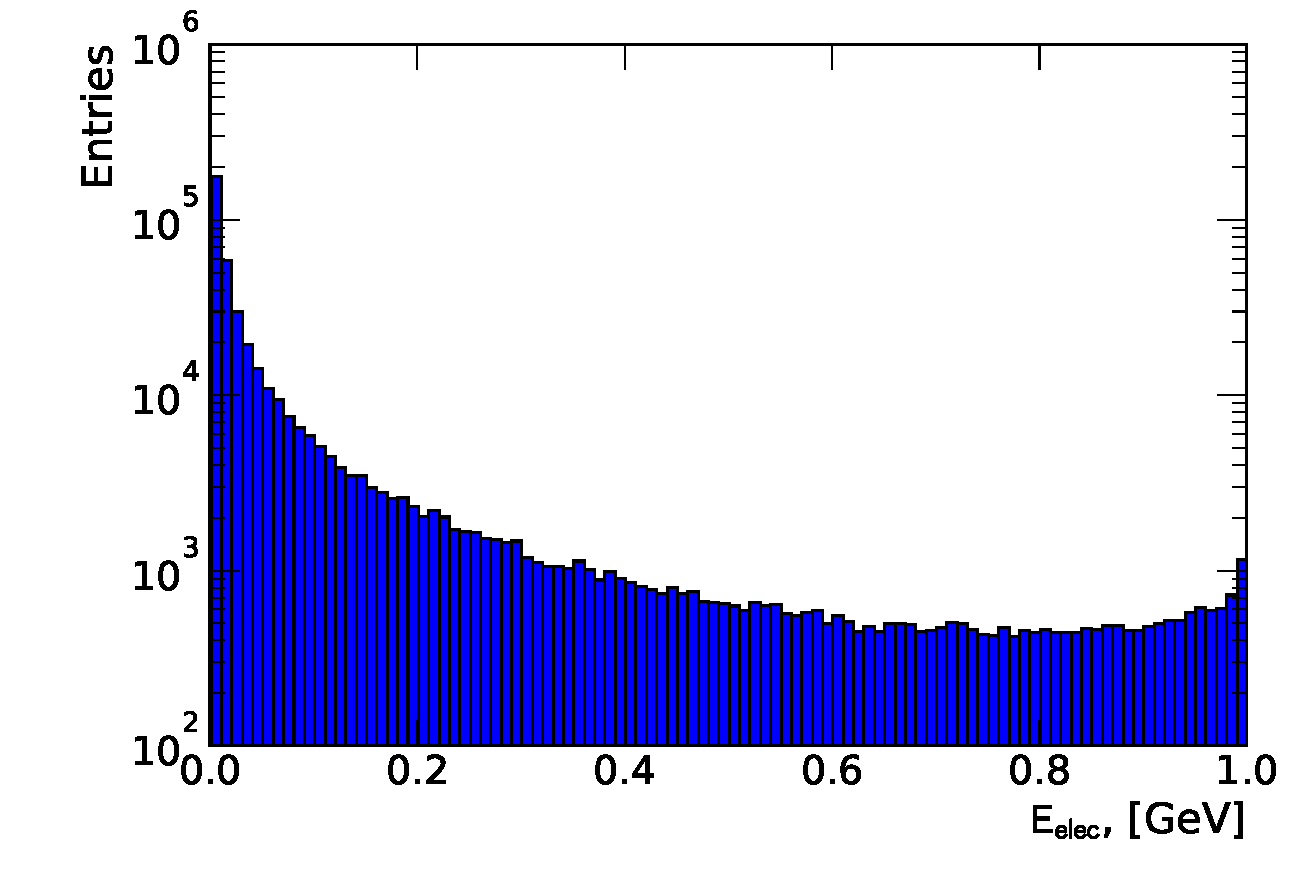
\includegraphics[width=0.8\textwidth]{MC/FSEnergy.pdf}
\caption{Distribution of shower energy used in production of 1000 GeV electrons.}
\label{fig:FSEnergy}}
\end{figure}

Performance of frozen showers is also depending on a lower limit of a method. 
Distribution of shower energies, used for production of high-energetic electron (1000 GeV in that case), is shown on a Figure ~. More than 50\% of them are having energy less than 20 MeV. Studies have showed, that Frozen showers are slower, than a standard Geant4 simulation for showers with energy 3 MeV. This is happening due to library non-binned structure for energy. This makes search of closest energy shower in a library slower, than simulation of shower with zero or one hit in a sensitive detector. 

\subsubsection{Generation of Frozen Showers library}

\begin{table}
\centering
\begin{tabular}{l|r}
\hline
\hline
\multicolumn{2}{c}{The general frozen showers parameters} \\
\hline
Detectors used            & FCAL1, FCAL2, FCAL3 \\
Type of the particle      & photons, electrons, neutrons \\
Energy range              &  $E_{\gamma}<10$~MeV,  $E_{e}<1000$~MeV,  $T_n<100$~MeV \\
Containment requirement   & $\Delta E_{shower} > 98\%$\\
\hline
\multicolumn{2}{c}{The library post-processing parameters} \\
\hline
Generation clustering cutoff & $(\Delta R_{cluster})^{2} < 25$ mm\\
Generation truncation cutoff & $R_{hit}^{2} < 50000$ mm, $\Delta E_{shower} < 1\%$\\
\hline
\hline
\end{tabular}
\caption{Main parameters used for the frozen shower libraries in FCAL }
\label{tab:MC_FS_params}
\end{table}

In a Frozen Shower method there are separate libraries for each particle and subdetector used. Showers should cover fully energy and pseudorapidity region and be able to describe data, that is needed during simulation. This is why 2 stages simulation approach have been used. The first stage takes initial particle parameters from a physical processes (ttbar or a single electron). 

The first stage is to take initial particle parameters, that later will be used in a library from a physical process. This is done using simulation of some process (e.g. ttbar or single electron). Every time, when particle becomes eligible for Frozen Showers, it parameters are saved in a HepMC format. Particles inside calorimeter tend to cluster tightly around initial track, so random truncation of initial particles is used to obtain better detector coverage. On the second stage, this primary particles are propagated through the calorimeter using standart Atlas simulation infrastructure. Resulted shower parameters are saved in a library. This procedure allows to take into account sampling fluctuations and charge-collection effects on a hit information automatically. Additionally, in order to save disc space as well as a memory consumption, hit information is compressed. This compression is done in a two steps, hit merging and truncation:
\begin{itemize}
\item if the distance between any two hits is smaller, than a given parameter $R_{min}$, then hits are merged into one deposit at the energy weighted center of them. This process is done iterativelly.
\item hits whose energies are below the fraction f of the total energy sum of all hits, are truncated. The energy of remaining hits is rescaled back to preserve the total deposited energy.
\end{itemize}

Unfortunately, for a Frozen Showers, generated for Run-1 monte-carlo, additional tuning of electron libraries was needed. This was done using reconstructed energy of electrons. Frozen Showers tend to underestimate fluctuations of energy loss, that is leading to a smaller electron resolution for a high energies. Correction is done by enlarging bin, corresponding to a gap position. Also, correction of the mean shift is done by scaling energy response of all showers. After this frozen showers are showing good agreement with full simulation. This procedure needs to be done every time, when something is changing in software. Because tuning is done manually, lots of a manpower is needed for each Monte Carlo mass production campaign.



\begin{figure}[h]
\center{
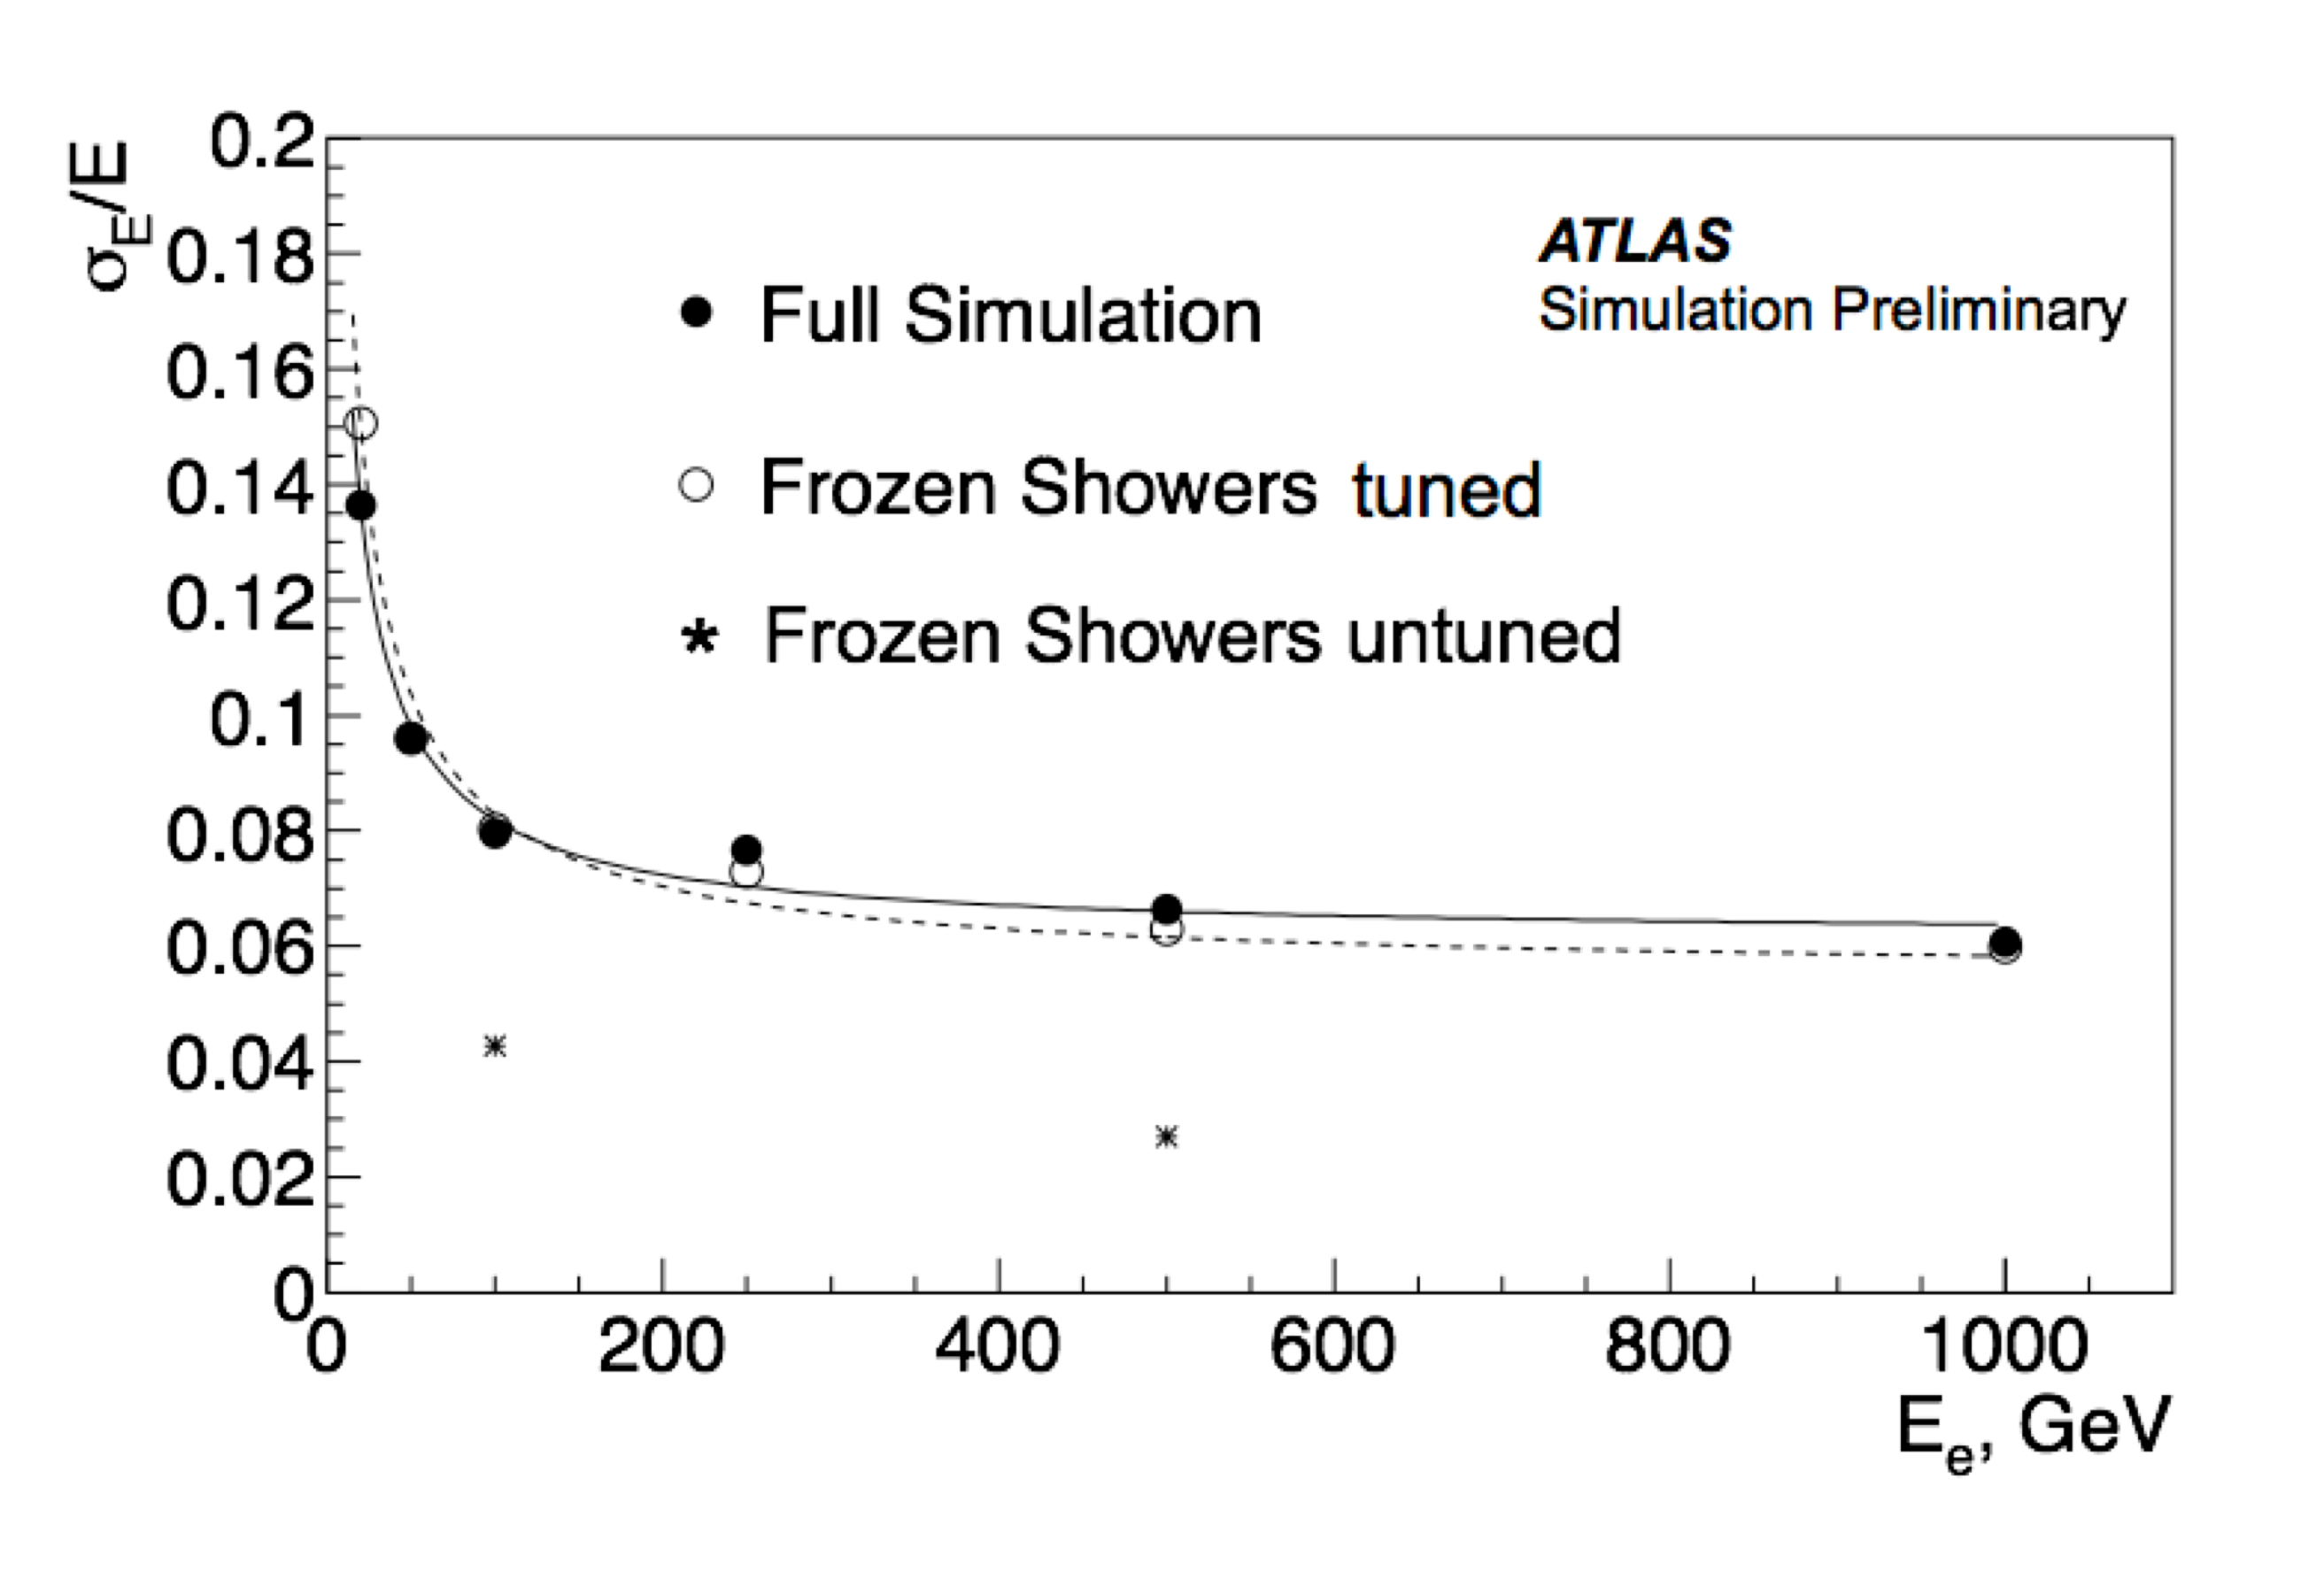
\includegraphics[width=0.7\textwidth]{MC/fs.png}
\caption{Electron resolution for full simulation, tuned and untuned frozen showers}
\label{fig:FS_resolution}}
\end{figure}

\subsubsection{Distance binning problem}
As it was mentioned before, process of library generation can be comlicated and take a lot of the time because of the needed tuning. In this subchapter possible ways to improve frozen showers performance have been studied. 
\begin{figure}
\center{
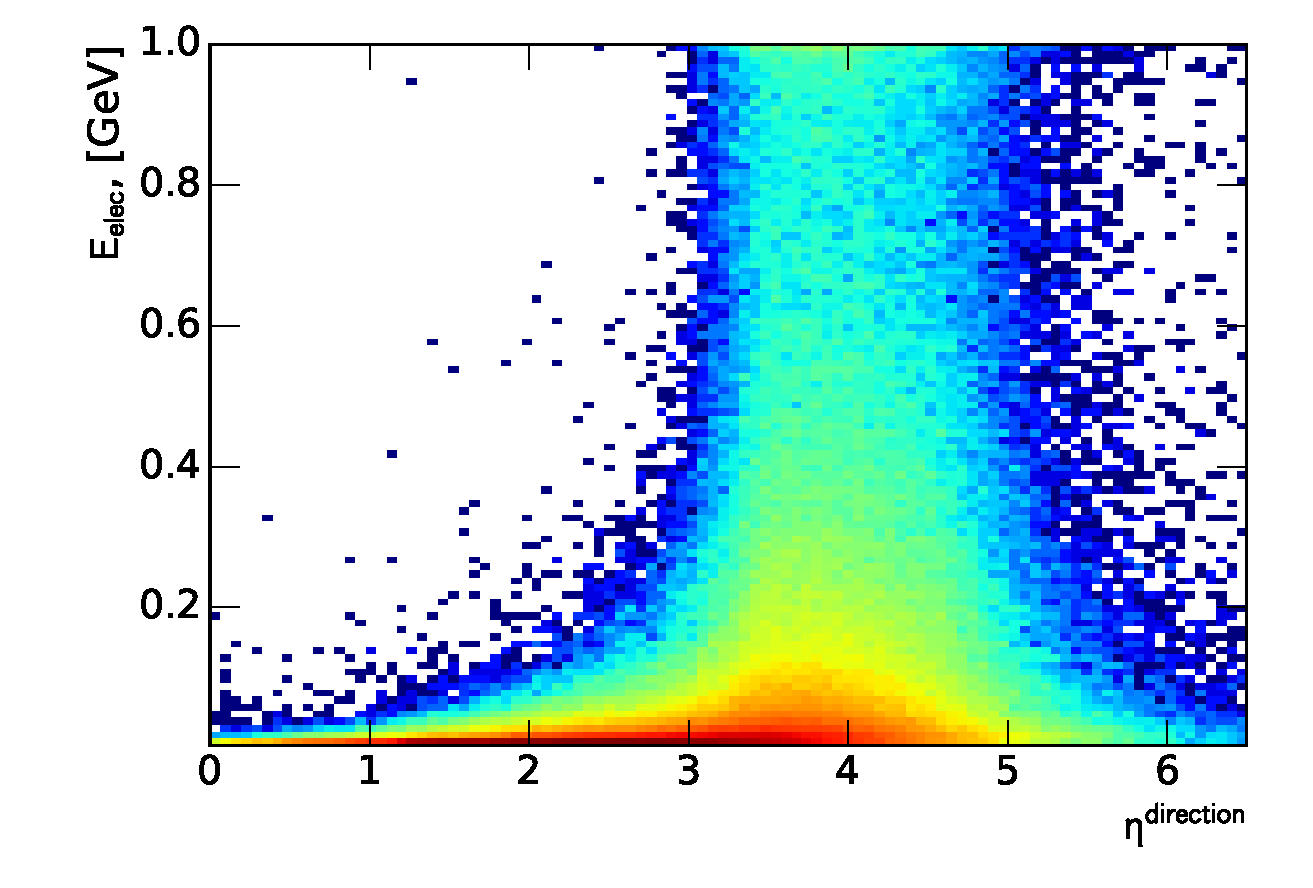
\includegraphics[width=0.8\textwidth]{MC/FSEtaMomVsEnergy.pdf}
\caption{Distribution of showers used in production of 1000 GeV electrons on shower energy vs $\eta_{momentum}$ plane.}
\label{fig:EtaMomVsEnergy}}
\end{figure}

As it was mentioned before, that there are two type of material used in a FCAL. Showers within them are giving different response, what is affecting overall reconstructed electron energy resolution.  At the first generations distance bin have been corresponding to LAr gap or dead material positions. During tuning bin with LAr was enlarged to gain a better agreement with full simulation. So, one of the basic ideas to improve frozen showers performance is to change a size of LAr gap in a library generation. 

It was decided to treat showers, that have been born near LAr gap and crossed it on a radiation length, in a same way with showers in sensitive material gap, and call them sensitive material showers. Oppositely, showers, that haven't crossed LAr gap, are called dead showers. This model leads to a bigger gap width by a definition. One of the possible ways to find this bin position automatically is to use machine learning tools. 

Machine Learning is a set of algorithms, what allows computers to learn and give a predictions without being specifically programmed. This is a modern field of computer science, that is wildly used in a different fields like computer vision, natural language processing, data science etc. There are two main types of machine learning algorithms: supervised, where example of desired output is given by the "teacher" and the goal is to learn a general rule, that maps inputs to outputs and unsupervised learning, then there are no labels given to algorithm, and algorithms is discovering hidden patterns in data. Initial data parameters of interest, that are used in algorithm to learn are called features. It is important to have right proper set of features and good training sample. 

From a geometrical point of view, one of the main parameter is a direction of the shower. Eta momentum distribution is showed on a Figure ~\ref{fig:EtaMomVsEnergy} . Most of the showers are collinear to an electron direction. Because of this it was decided to use as a training sample simulation results for electrons with energies less than 1 GeV and momentum uniformly distributed between eta 3.0 and 4.0. This allowing to study equally low and high energy showers equally.

\begin{figure}[h]
\begin{minipage}[h]{0.49\linewidth}
\center{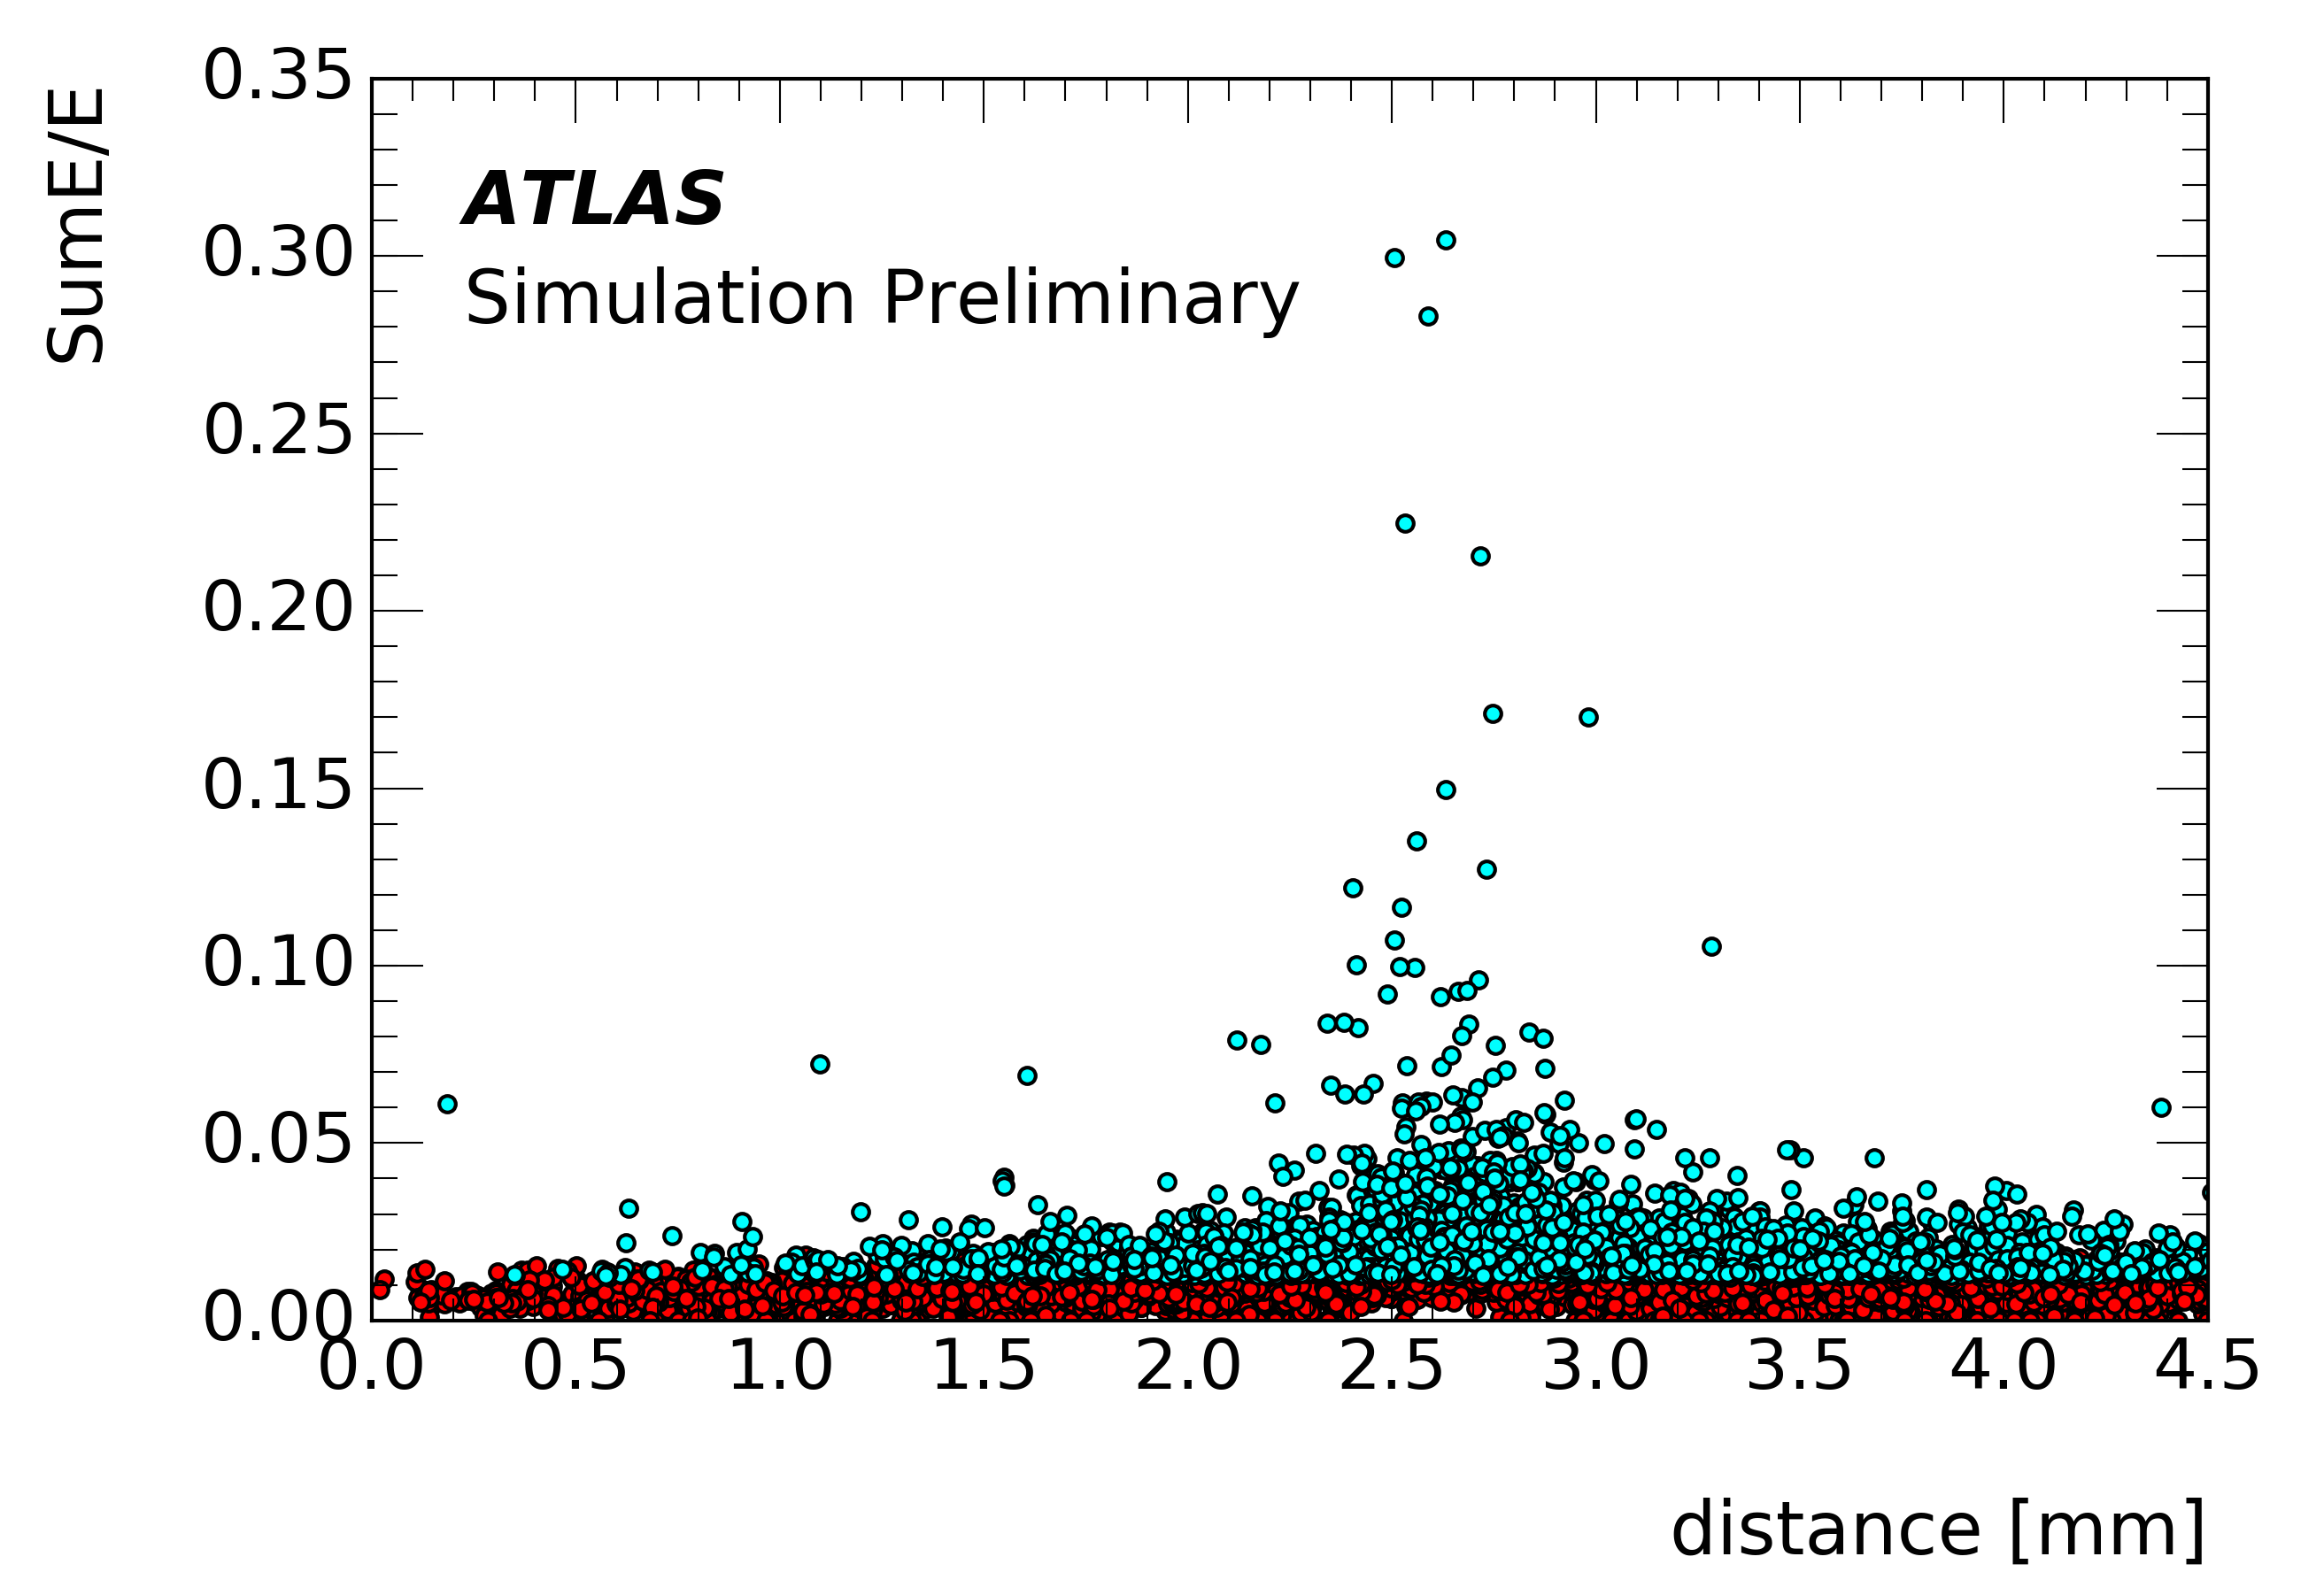
\includegraphics[width=1.\linewidth]{MC/firstClassifier.png} \\ a)}
\end{minipage}
\hfill
\begin{minipage}[h]{0.49\linewidth}
\center{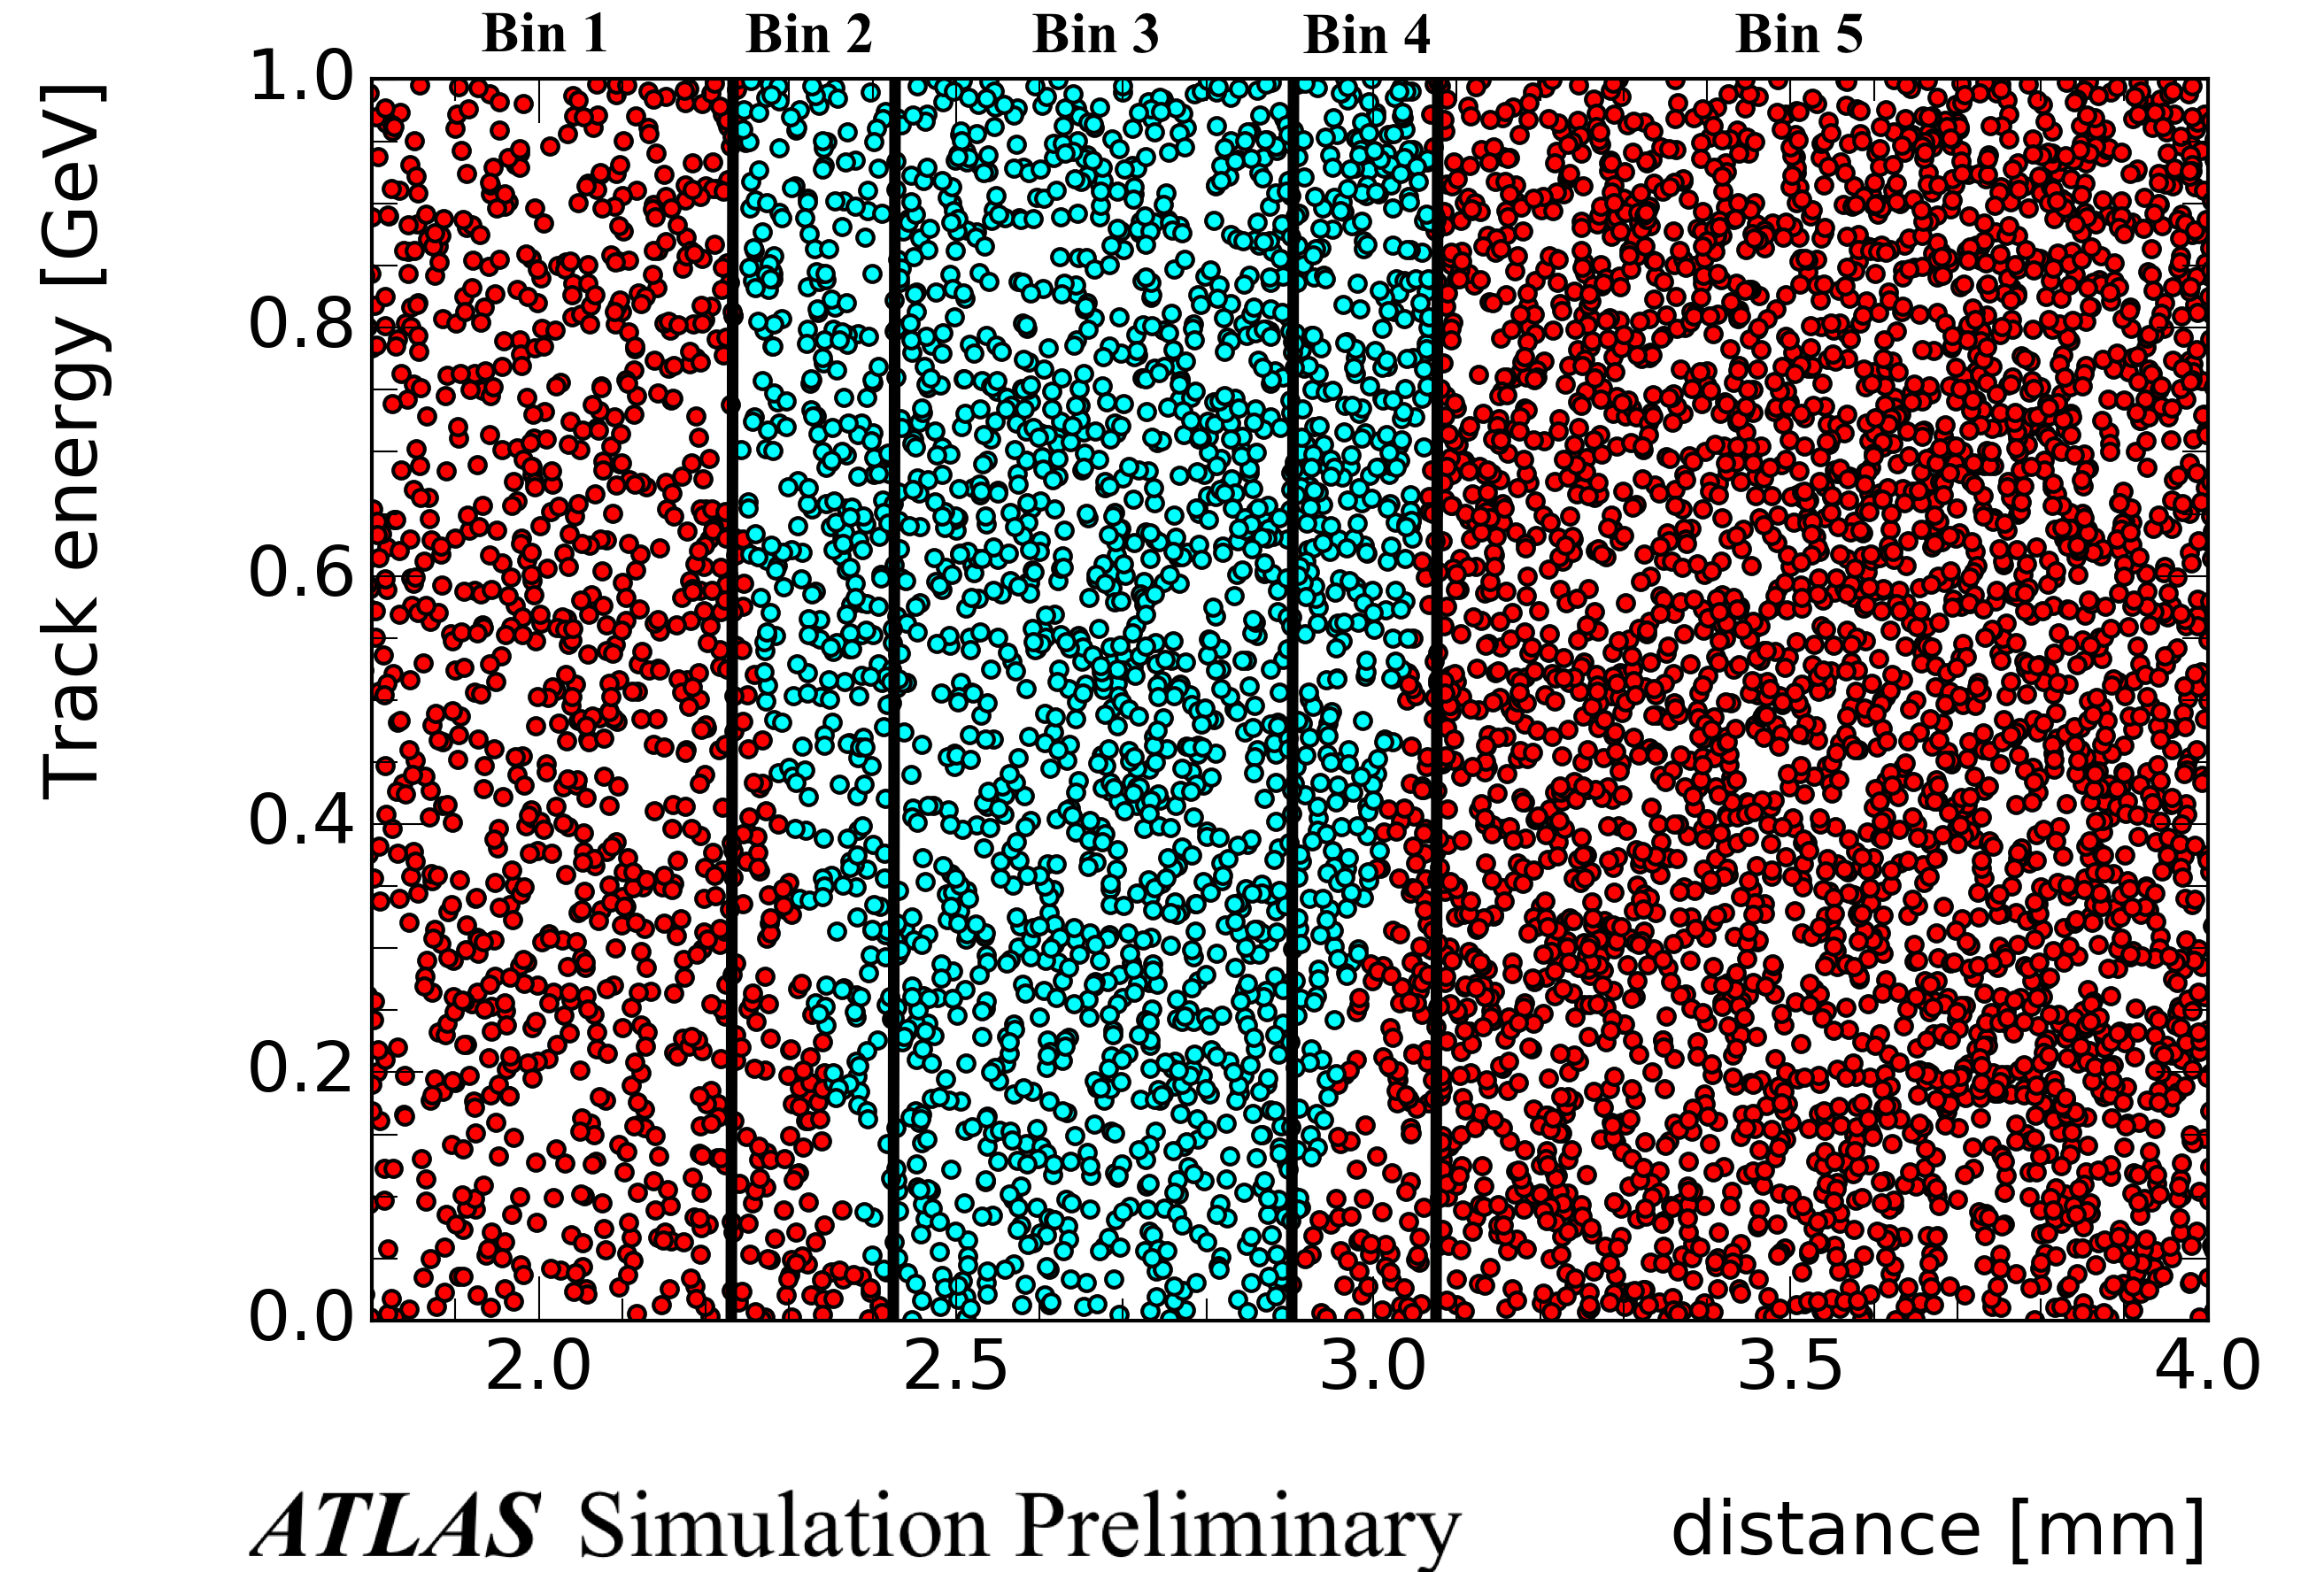
\includegraphics[width=1.\linewidth]{MC/secondClassifier.png} \\ b)}
\end{minipage}
\caption{Results of machine learning for a) first classifier b) second classifier. Cyan dots are corresponding to sensitive material showers, red - dead material showers}
\label{fig:Class}
\end{figure}


From out definition of 2 classes of showers, it is simple to construct a pre-labelled training sample. This is done by reducing initial sample and taking showers near rod center and inside liquid argon gap. Output of this classifier, that was trained on with sample with shower features, such as energy response and number of hits, than can be used to expand our labels to a full distance range. Than it can be used as an input to a second classifier, which will separate two types of showers using particle parameters, such as energy and distance to a rod center. For a first step decision trees have showed good classification efficiency (around 97\%). For a second classifier support vector machines have been used. This method is trying to reconstruct a hyperplane, that is dividing two classes. Outputs of both of this classifiers are shown on a figure . New gap position is determined using borders of hyperplane. This procedure is giving expected from the initial model results. Gap is wider, than and original one. It is also getting bigger with bigger energy, because of the radiation length growth. 
Validation results for two different eta bins are shown on figure ~ a) and b). In a bin this new binning is performing better, than original one without any additional tuning. Unfortunately this is not true for all of the bins, as we can see on a figure ~ b). This eta bin have showed worst performance for a new binning, but it is performing still better, than original binning without tuning.

\begin{figure}[h]
\begin{minipage}[h]{0.49\linewidth}
\center{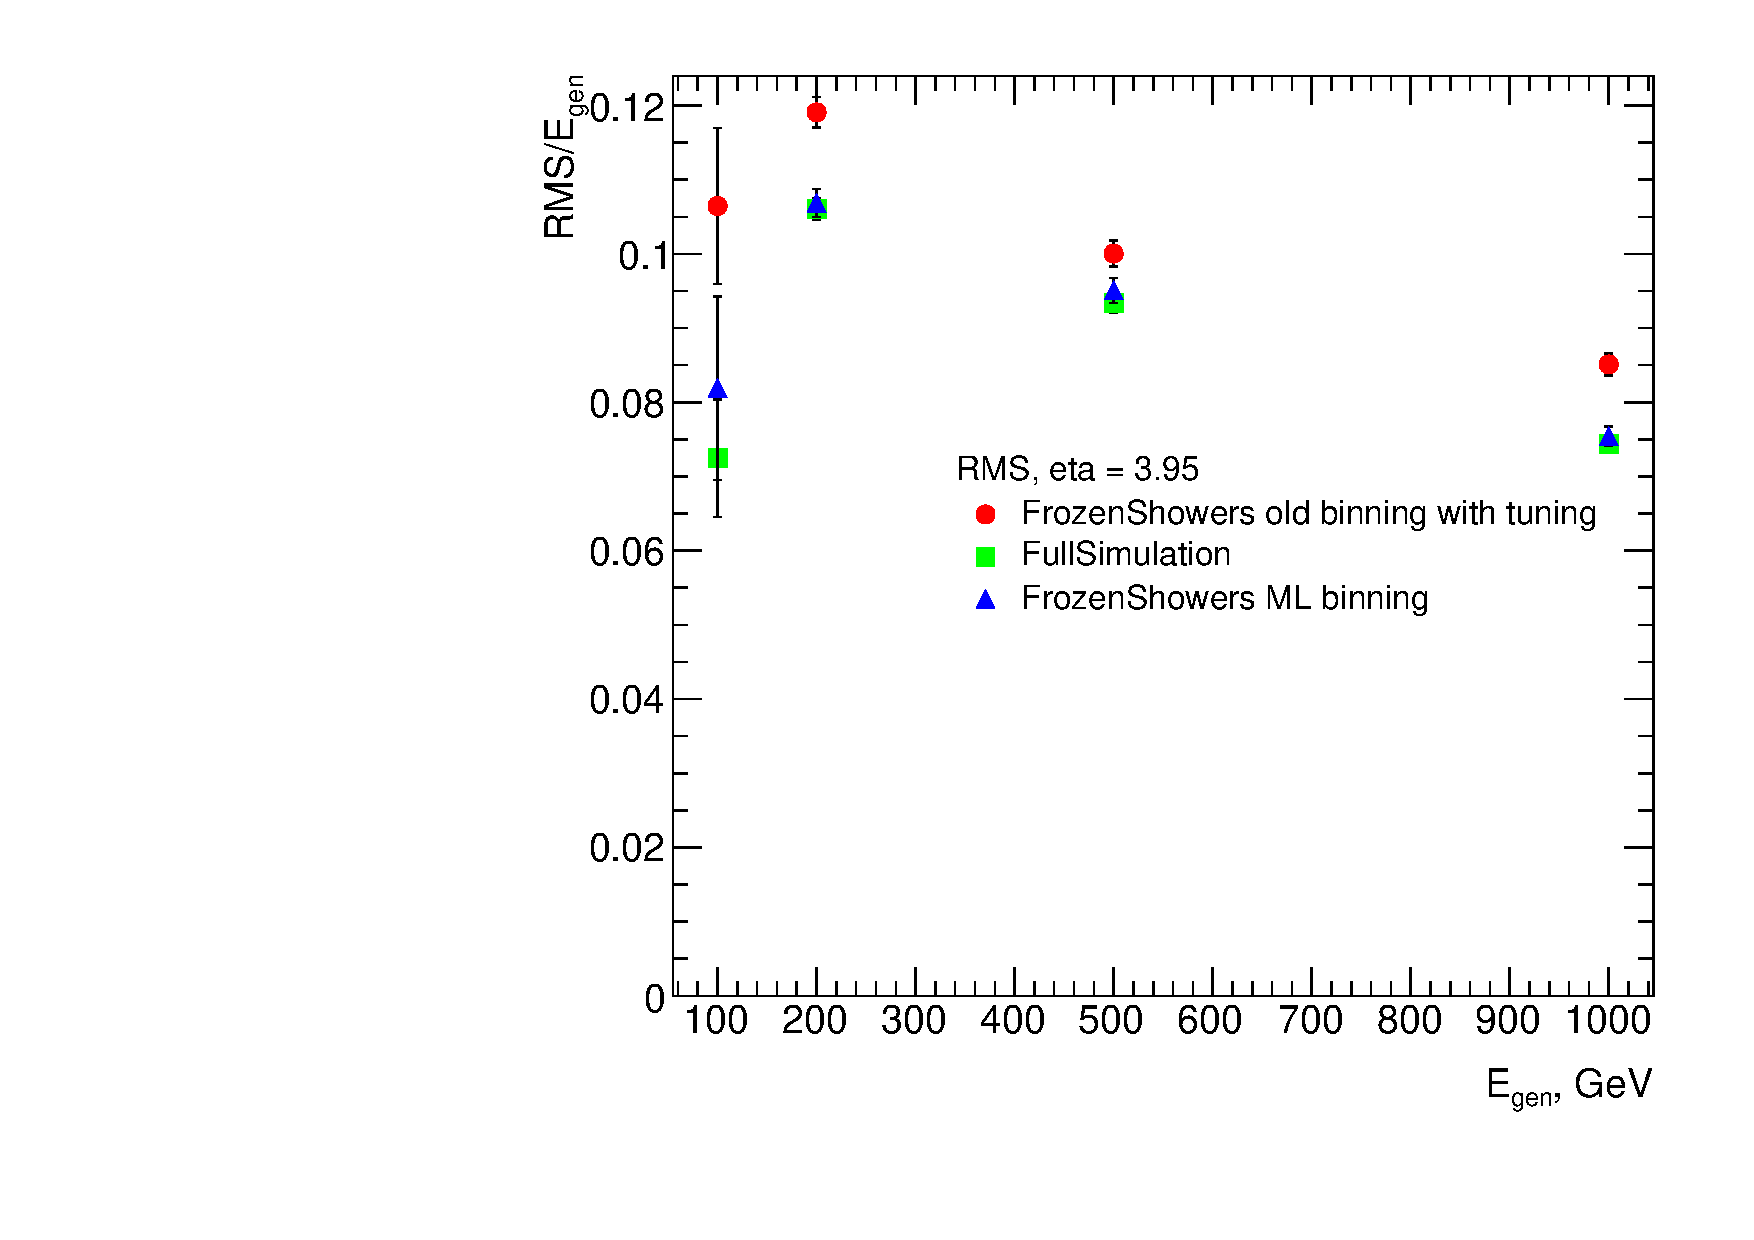
\includegraphics[width=1.\linewidth]{MC/rms3p95.pdf} \\ a)}
\end{minipage}
\hfill
\begin{minipage}[h]{0.49\linewidth}
\center{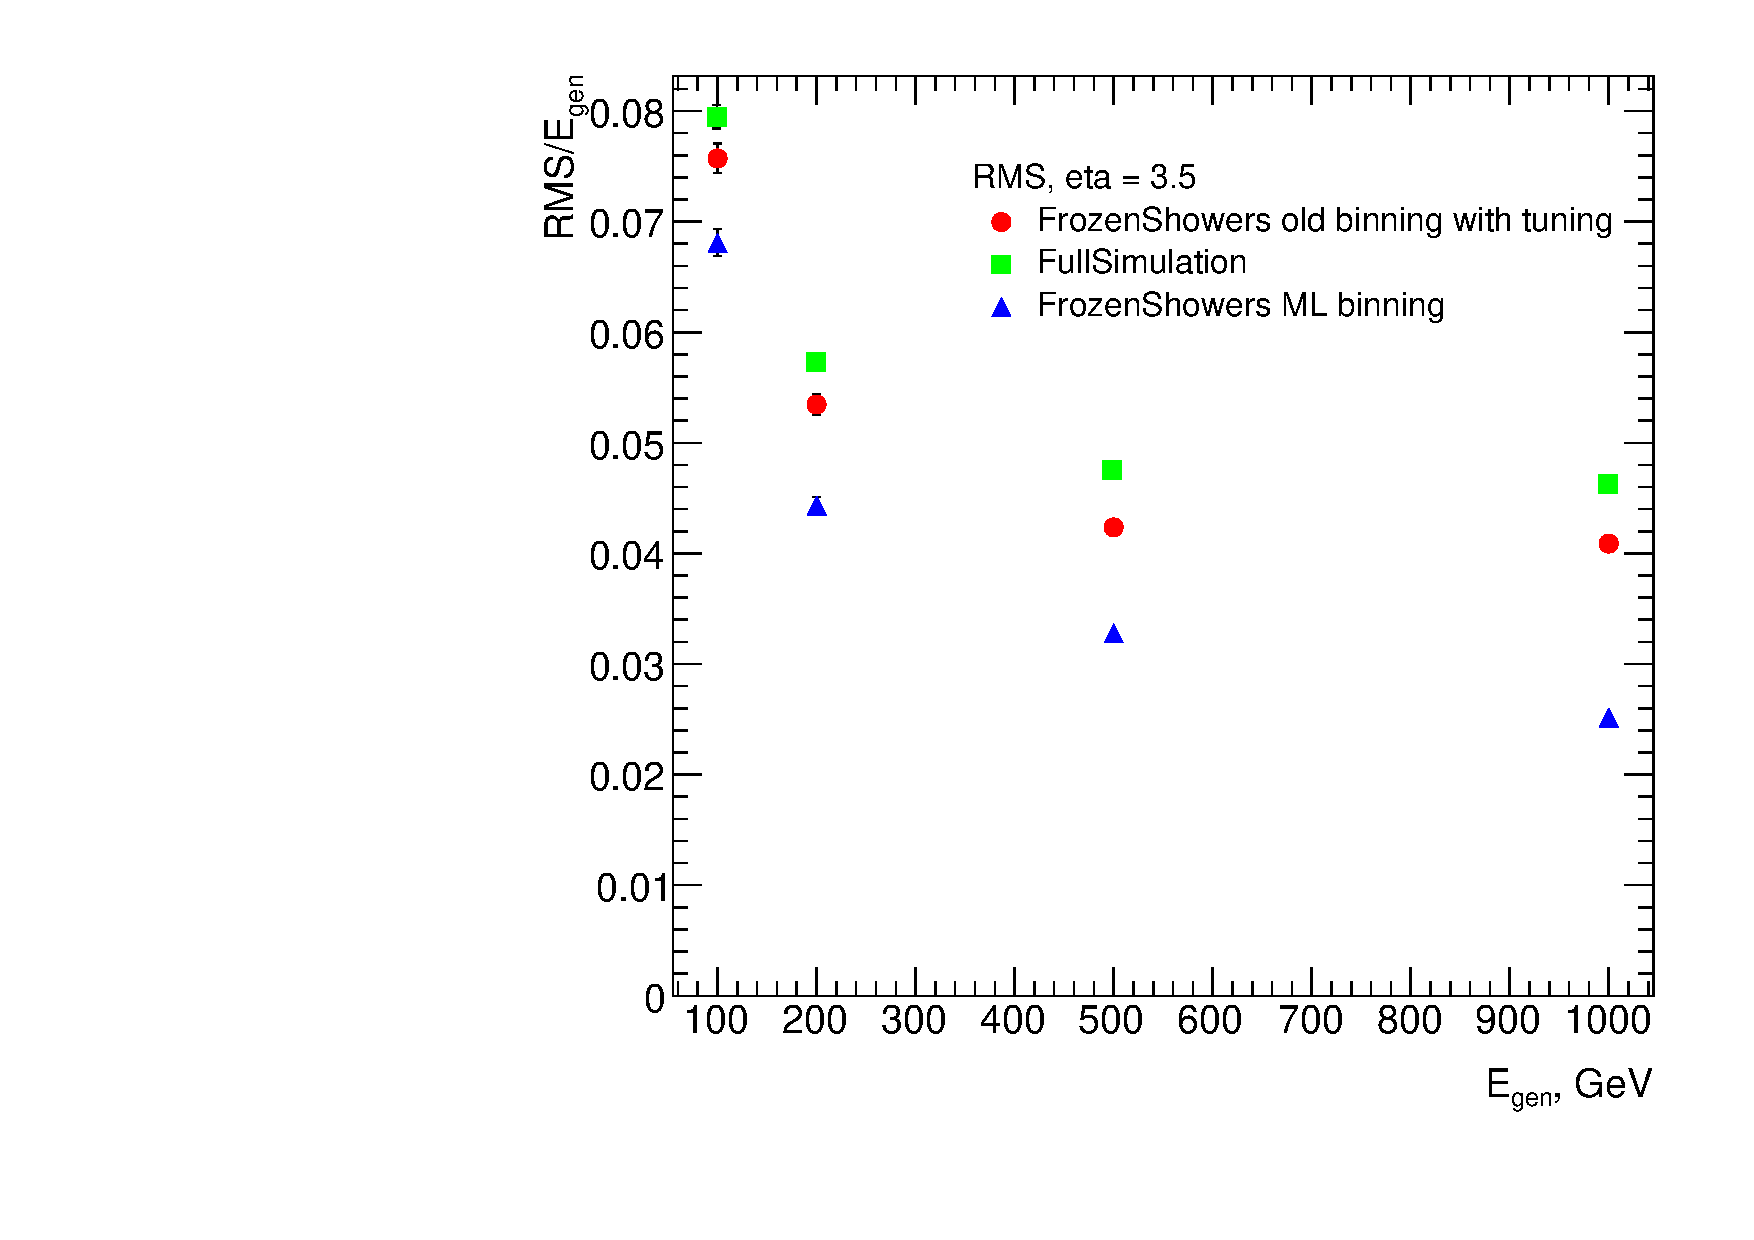
\includegraphics[width=1.\linewidth]{MC/rms3p5.pdf} \\ b)}
\end{minipage}
\caption{Resolution of reconstructed electrons for full simulation, new libraries with ML binning and old tuned libraries with original binning for a) eta =3.95 b)eta=3.5 }
\label{fig:Class}
\end{figure}

This binning was used in a production of new libraries for Monte Carlo in a Run-2. It is planned to use more precise training sample for a future iterations of this procedure for improving performance of outlying eta bins.

  \chapter{Frozen Showers}\label{chap:FS}
\minitoc


As it was mentioned in Chap.~\ref{chap:MC}, fast simulation techniques are an essential part of the Monte-Carlo production in the \atlas experiment. The typical time needed for simulating a $t\bar{t}$ event is around 1 minute, and most it is spent on the simulation of particle interaction in the calorimeters. This motivates the development of fast calorimetry techniques, allowing to describe calorimeter response.

In this chapter a Frozen Showers method for the forward calorimeter simulation is described. The first section gives a small introduction to the method. In the next section properties of the electron shower in the FCAL are showed. In the Sec.~\ref{sec:FSProdUse} the use of method is explained. The Sec.~\ref{sec:MLBinning} introduces a new method of finding the bin size for a libraries. Finally, in the last section, the validation of Frozen Showers is showed.

\section{Introduction}
Frozen showers is currently the main fast calorimeter simulation approach used at \atlas experiment\cite{FS}.  This method uses pre-simulated "frozen" showers. This allows to reduce the time spent on a simulation of a large amount of low energy sub showers. This method gives a 25\% speedup in simulation. It is required to have in advance generated libraries for each detector and particle used in this method. 

For each shower in the library its lateral and transverse size and a list of the all energy deposition inside the sensitive material (hits) with information about their energy, position and time are stored. During simulation, if the energy of a secondary electron falls below the cut-off energy it is replaced by a shower from a library, as shown in Fig.~\ref{fig:MC_FS_method}. Main parameters used in \atlas simulation are summarized in a Tab.~\ref{tab:MC_FS_params}, where FCAL1 and FCAL2 are the first two froward calorimeters (see Sec. \ref{sec:forwardCalo}) and $E_{\gamma}<10$, $E_{e}<1000$, $T_n<100$ are the maximum energies of photons, electrons and neutrons used in the method. 

Since currently the Frozen Showers method is used only for FCAL, this chapter will fully concentrate on optimisation of Frozen Showers in forward calorimeter.

\begin{figure}[!tbp]
\center{
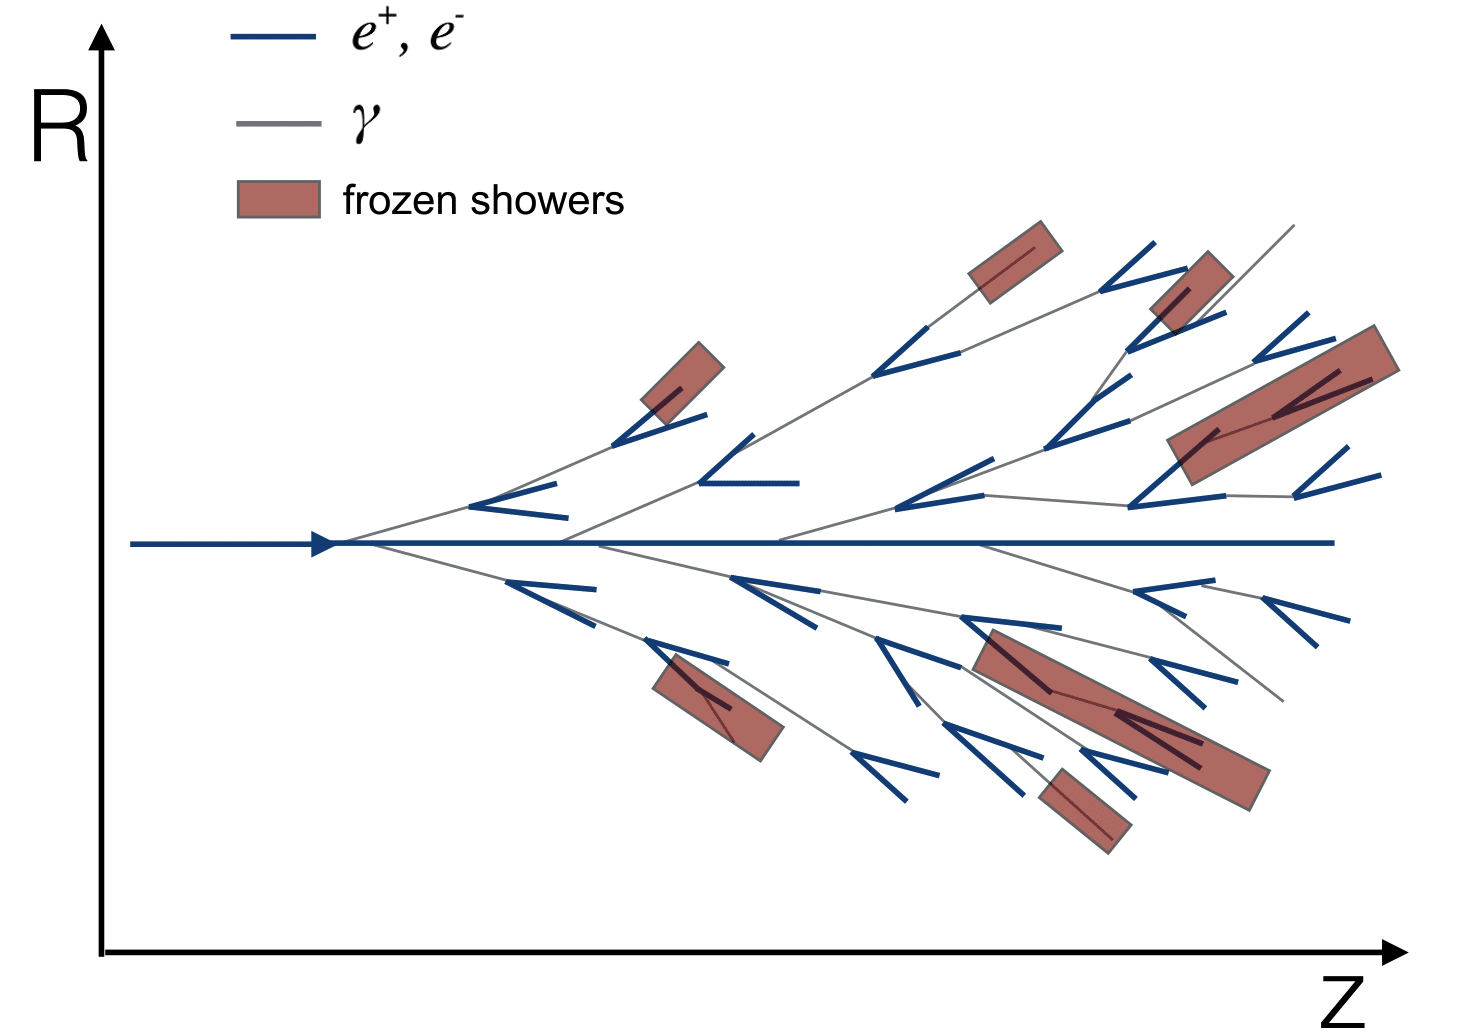
\includegraphics[width=0.9\textwidth]{MC/FSMethod2.png}
\caption{Diagram showing the shower substitution of the low-energy electron, during the high-energy particle simulation. Some of the showers from a particles, substituted by frozen showers method marked by a red squares}
\label{fig:MC_FS_method}
}
\end{figure}

\begin{table}[!tbp]
\caption{Main parameters used for the frozen shower libraries}
\label{tab:MC_FS_params}
\centering
\begin{tabular}{l|r}
\hline
\hline
\multicolumn{2}{c}{The general frozen showers parameters} \\
\hline
Detectors used            & FCAL1, FCAL2\\
Type of the particle      & photons, electrons, neutrons \\
Energy cut-off            &  $E_{\gamma}<10$~MeV,  $E_{e}<1000$~MeV,  $E_n<100$~MeV \\
\hline
\end{tabular}
\end{table}

\section{Properties of electron showers in FCAL}\label{sec:FSproblem}




%\begin{figure}[!b]
%\center{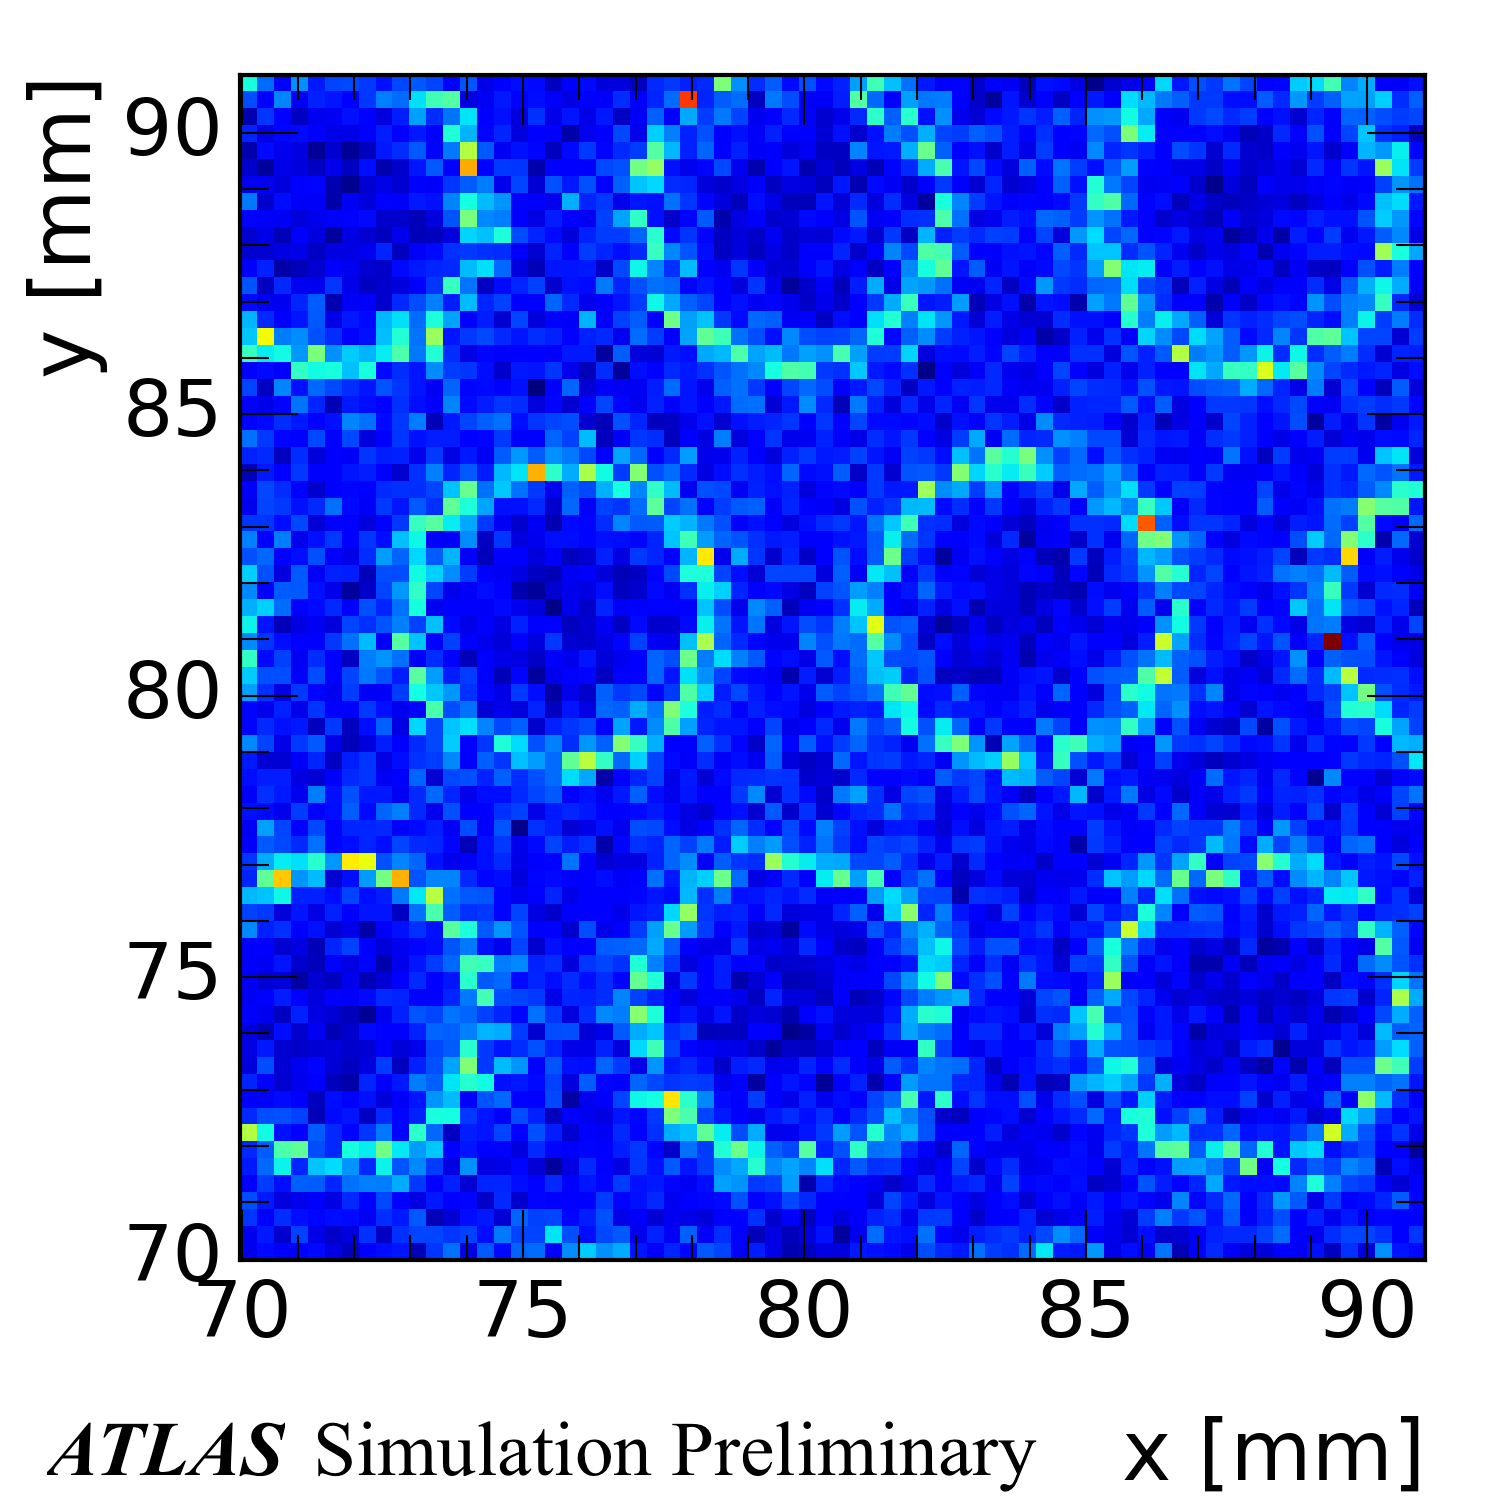
\includegraphics[width=0.5\linewidth]{MC/xySumE.png} }
%\caption{Shower energy response histogram in the x vs y plane for electrons, generated with uniformly distributed x and y and energy less than 1 GeV. Light circles are corresponding to a showers, started inside a LAr gaps with on average higher energy response, while the dark parts are corresponding to dead material respectively with smaller sum of the "hits" energy. }
%\label{fig:FSFluctuations}
%\end{figure}

\begin{figure}[!tbp]
\begin{minipage}[h]{0.49\linewidth}
\center{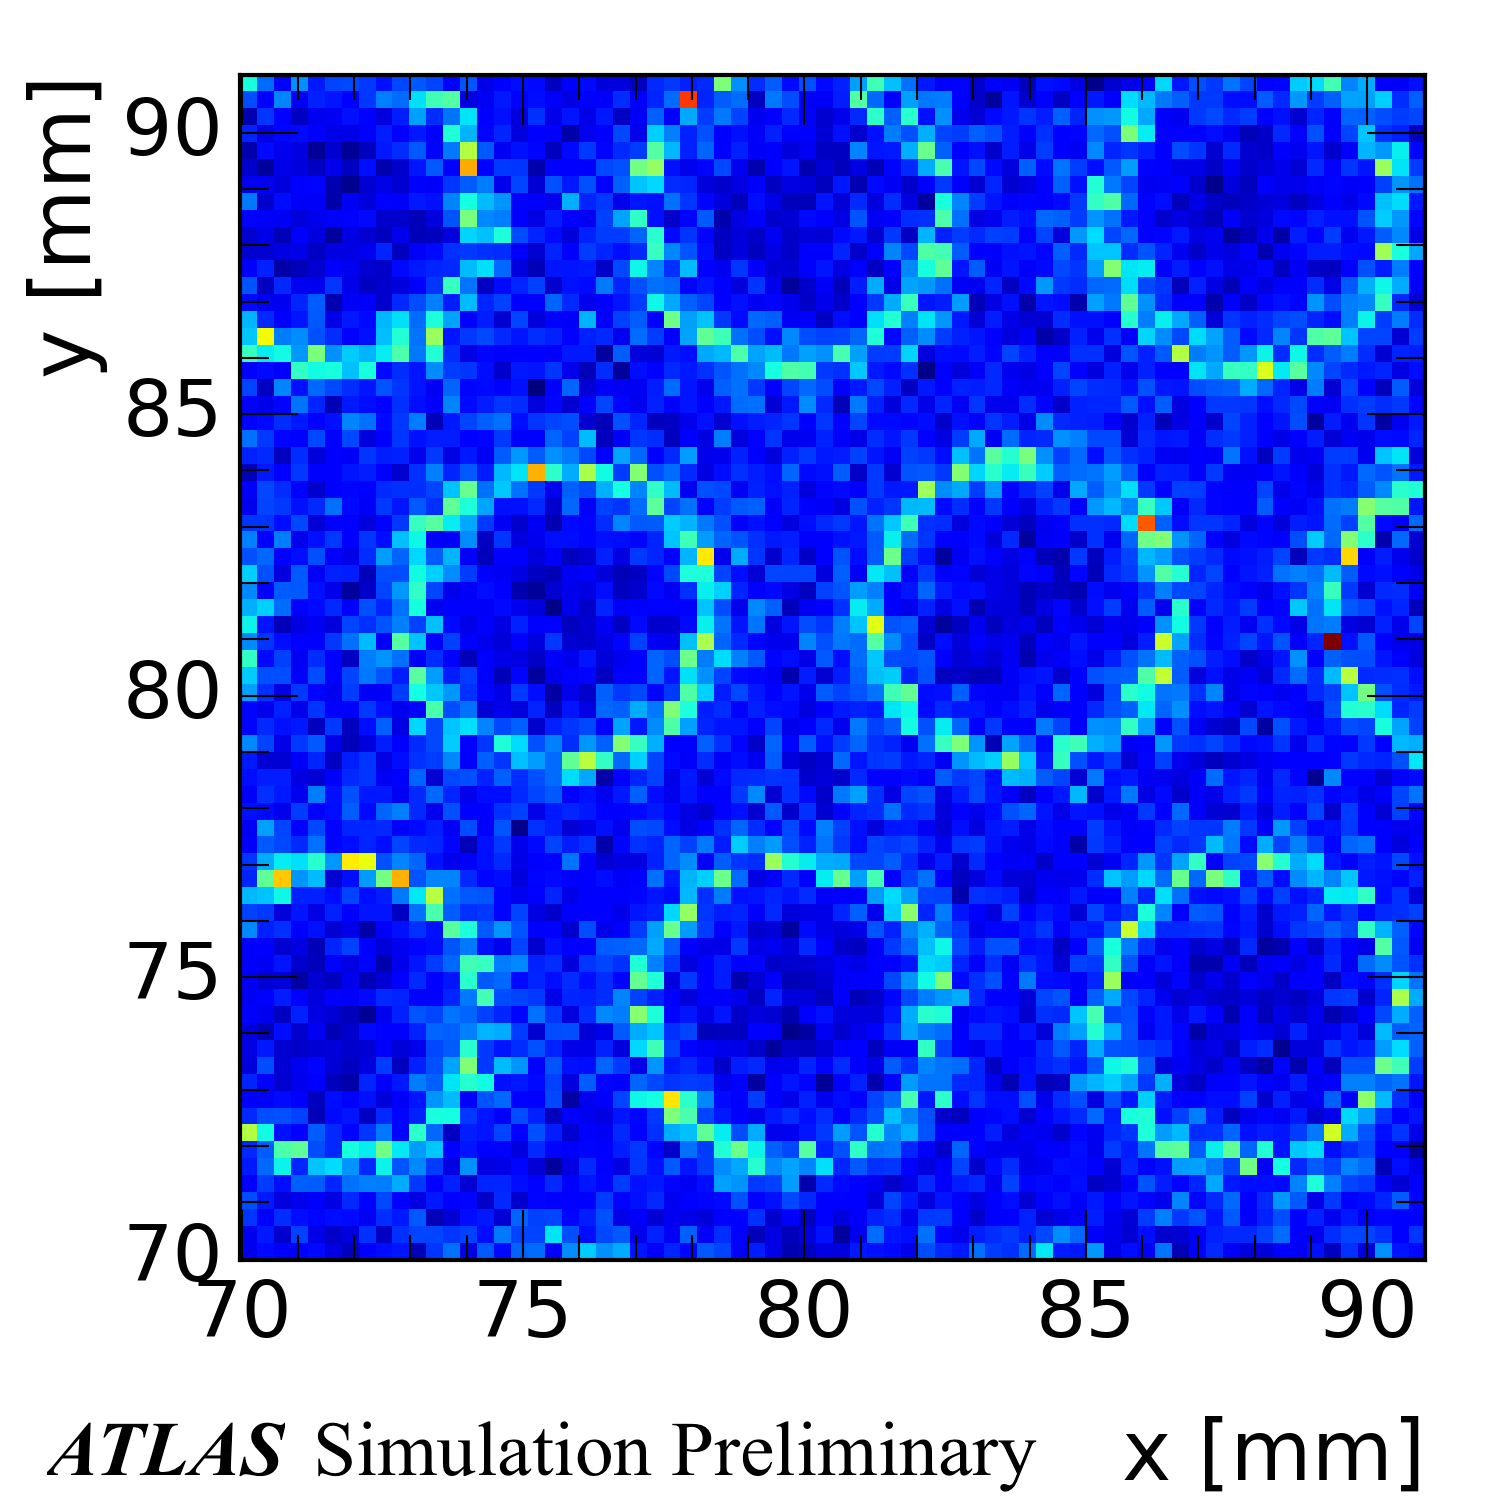
\includegraphics[width=0.9\linewidth]{MC/xySumE.png} \\ a)}
\end{minipage}
\hfill
\begin{minipage}[h]{0.49\linewidth}
\center{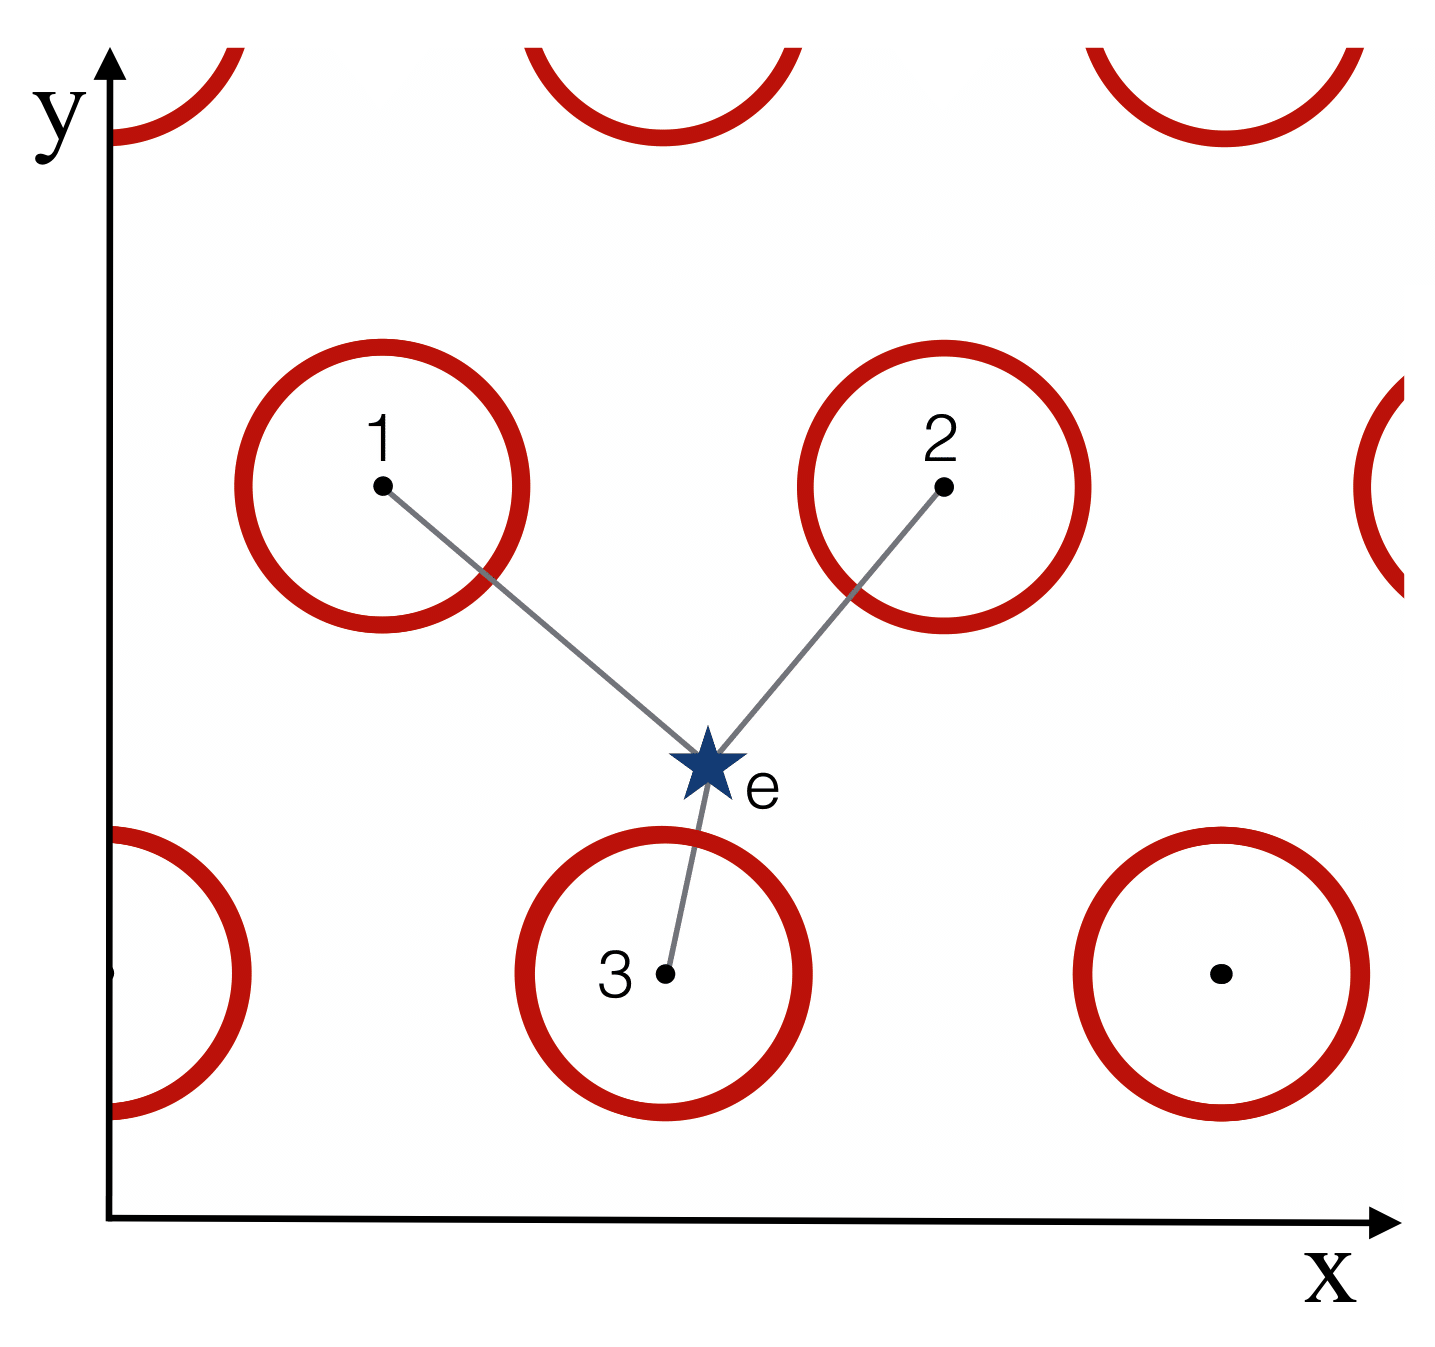
\includegraphics[width=0.9\linewidth]{MC/DistanceCalculation.png} \\b)}
\end{minipage}
\caption{ a) Shower energy response histogram in the transverse (x vs y) plane for electrons, generated with uniformly distributed x and y and total energy less than 1 GeV. Light circles correspond to showers, starting inside the LAr gaps with on average higher energy response, while the dark parts correspond to dead material with smaller sum of the "hits" energy respectively.
b) Distance to the closest rod center scheme $d_{rod} = min( d(1,e), d(2, e), d(3, e))$, where 1,2,3 are the positions of the rod centers and e is the position of initial electron. The rod centers and liquid argon gaps are shown by black dots and red circles respectively.}
%\caption{Distribution a) electron energies and b) mean number of hits in a shower vs energy of electron for electrons with energy less than 1 GeV coming from initial electron with energy 1 TeV. }
\label{fig:FSFluctuations}
\end{figure}


\begin{figure}[!tbp]
\begin{minipage}[h]{0.49\linewidth}
\center{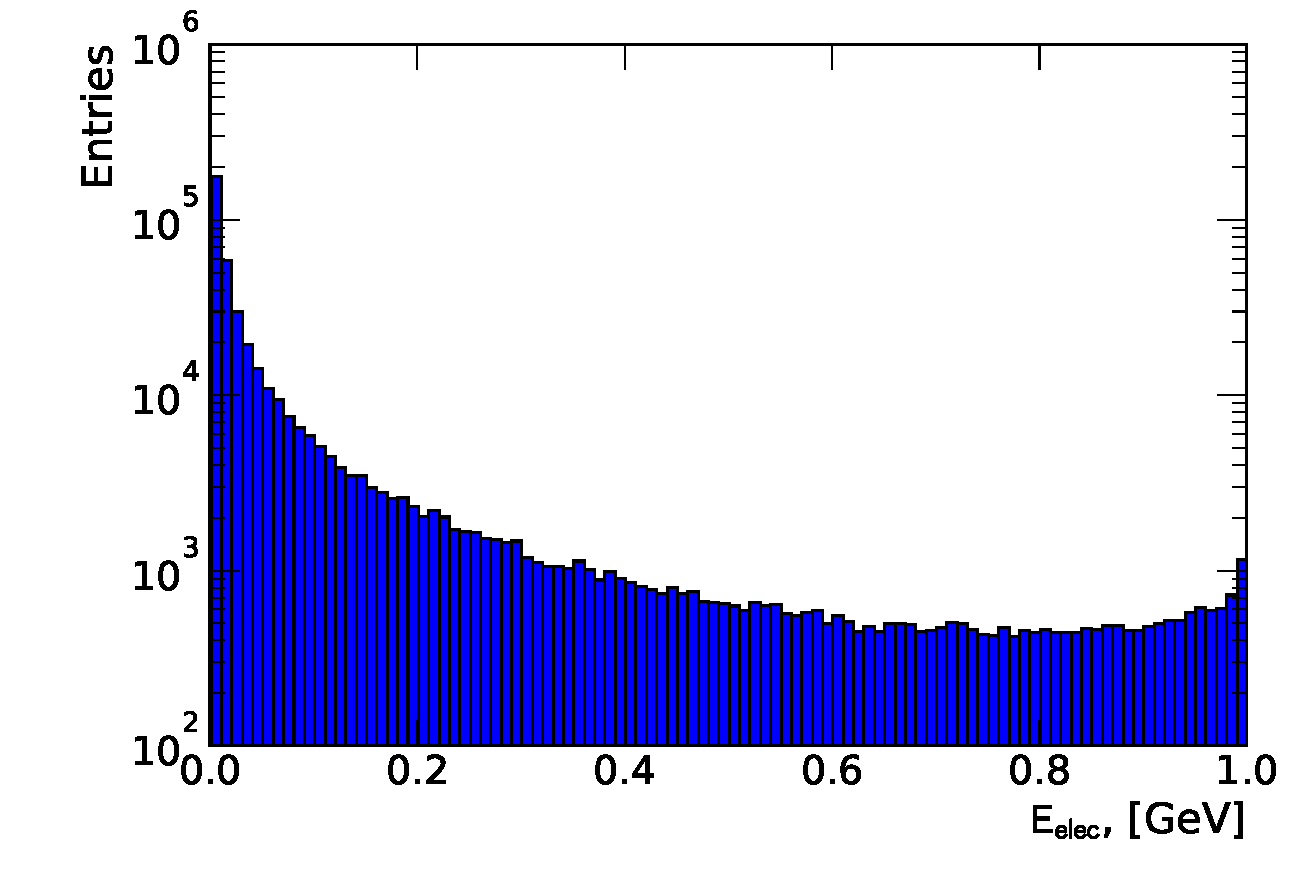
\includegraphics[width=1.0\linewidth]{MC/FSEnergy.pdf}  \\ a)}
\end{minipage}
\hfill
\begin{minipage}[h]{0.49\linewidth}
\center{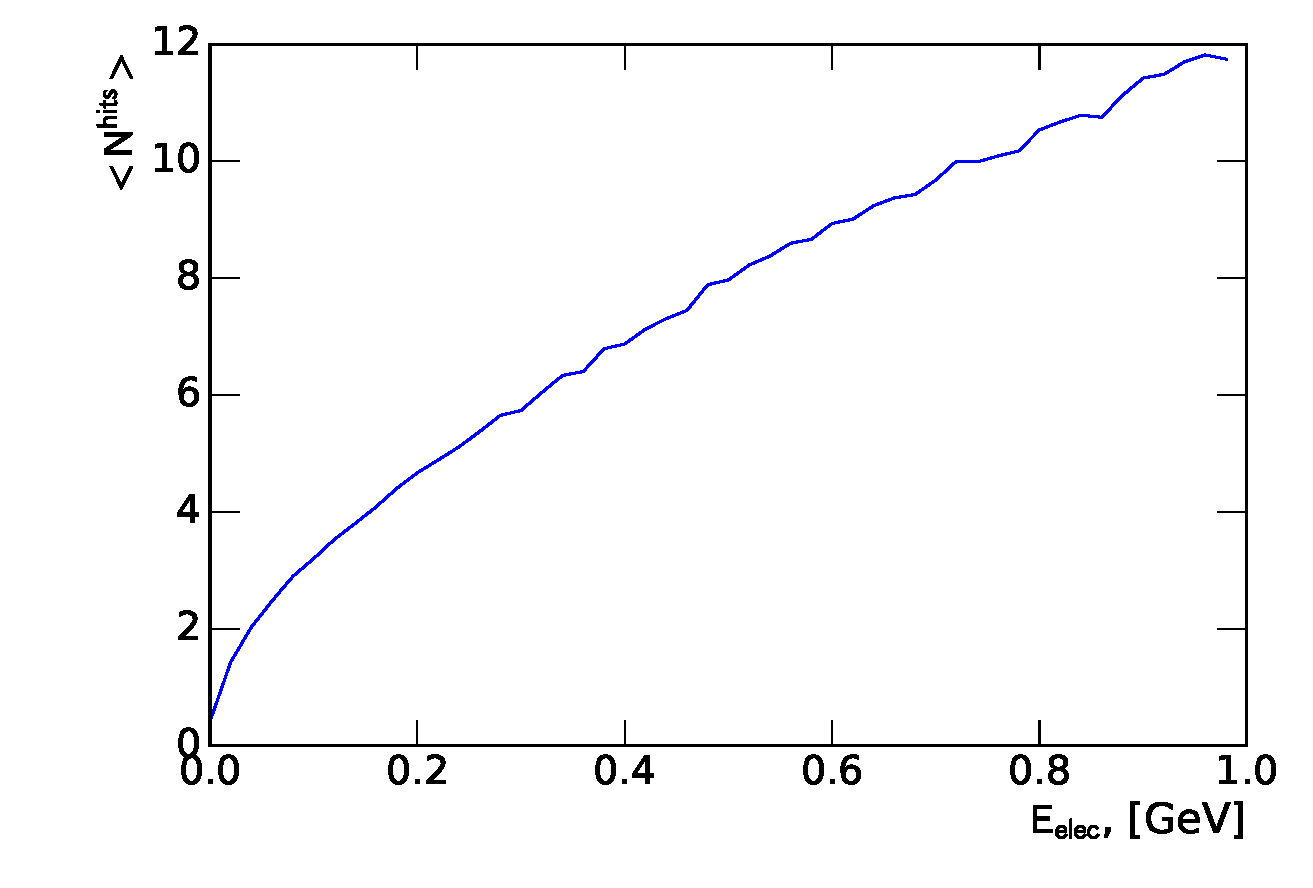
\includegraphics[width=1.0\linewidth]{MC/nHitsMean.pdf} \\ b)}
\end{minipage}
\caption{Distribution  of the a) electron energies and b) mean number of hits in the shower vs energy of electron for electrons with energy less than 1 GeV originating from 1 TeV initial electron.}
\label{fig:TrackEnergy}
\end{figure}

The fast simulation of  the forward calorimeters is a complicated task due to their complex structure. As it was mentioned in Sec.~\ref{sec:forwardCalo} FCAL consists of hexagonal absorber cells with an anode tube and cathod rod in the cell center and the liquid argon in the gap between rod and tube. In order to simulate the resolution of high-energy electrons, an efficient fast simulation technique should take into account this large amount of non-uniformly distributed sensitive material.

The electron energy resolution for this calorimeter can be written as:
\begin{equation}\label{eq:EMResoultion}
\frac{\sigma}{E} \approx \frac{1}{\sqrt{E}}	\oplus \frac{1}{E} 	\oplus const,
\end{equation}
where $\oplus$ indicates the quadratic sum. The first term is the 'stocastic term', which includes intrinsic shower fluctuations, the second  one takes into account readout noise effects and pile-up fluctuations. The constant term is connected to non-uniformities in the detector, causing large fluctuations of the energy loss. The energy resolution of high-energy electrons is mostly dominated by the constant term. 

Fluctuations due to the detector design are visible in the simulation of low energy electrons, generated inside different points in the forward calorimeter. The shower energy $E^{shower}$ distribution in the transverse x vs y plane is shown on Fig.~\ref{fig:FSFluctuations} a). The shower energy is defined as:
\begin{equation}
E^{shower}=\sum E_i^{hits},
\end{equation}
where $E_i^{hits}$ is the energy of the i-th hit in shower shower inside the sensitive material. The periodic structure resembles the calorimeter design, where the light circles correspond to gaps with liquid argon, which are acting as sensitive material. Introduction of distance to the closest rod center, calculated as shown in Fig.~\ref{fig:FSFluctuations} b) allows to catch this periodic structure.

A typical electron substituted by frozen shower coming from simulation of high-energy electrons has a relatively small energy (Fig.~\ref{fig:TrackEnergy} a). The mean number of deposits in the sensitive material in a "frozen" shower is around 5 and this value rises with the electron energy (Fig.~\ref{fig:TrackEnergy} b).  Fig.~\ref{fig:FSProduction} presents the distribution of the distance to a closest rod center vs shower energy for showers from electrons with energy below 1 GeV originating from initial electrons with an energy of 1 TeV. The liquid argon gap is marked by red lines. There is visible peak in showers energies for the region around liquid argon gap. The similar structure is also visible in a number of hits  (Fig. ~\ref{fig:ShowerProp} a) and the standard deviation of energy of the hits in the shower (Fig. ~\ref{fig:ShowerProp} b) distributions. The magnitude of the peak depend on the electron energy and is higher for the low energies (Fig. ~\ref{fig:FSProduction2} a) and less significant for higher energies (Fig. ~\ref{fig:FSProduction2} b).  This fact combined with energy distribution states the importance of a proper simulation of non-uniformities for showers coming from a low energy electrons.





\begin{figure}[!tbp]
\center{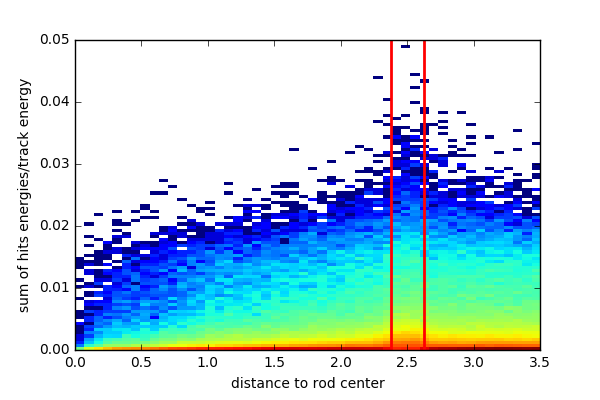
\includegraphics[width=1.\linewidth]{MC/fullBinningScatter.png} }
\caption{Distribution of distance to the closest rod center vs shower energy for electron showers created by electrons with energy less than 1 GeV originating from the initial electrons with energy 1 TeV in distance to the closest rod center vs shower energy plane. Position of the liquid argon gap is noted by a red lines. }
\label{fig:FSProduction}
\end{figure}

\begin{figure}[!tbp]
\begin{minipage}[h]{0.49\linewidth}
\center{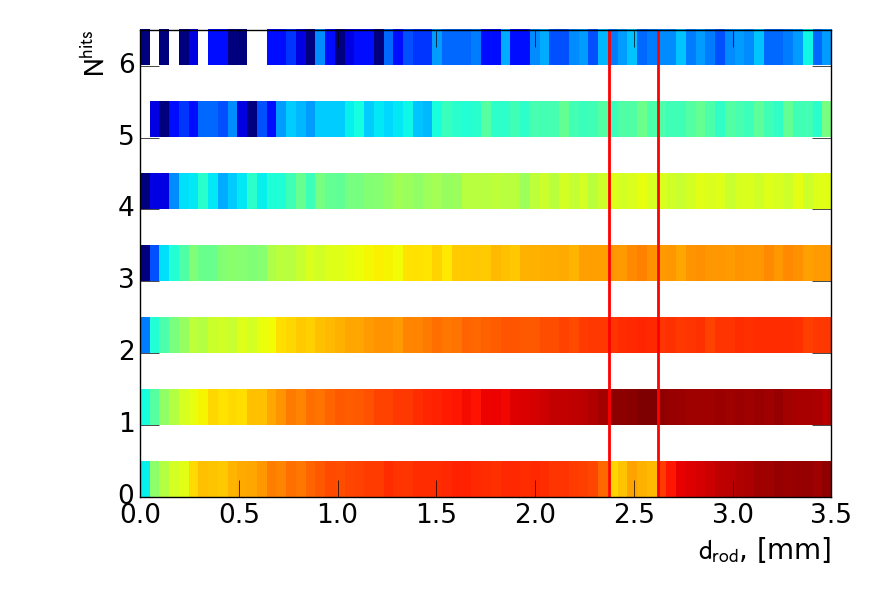
\includegraphics[width=1.0\linewidth]{MC/nHits.png}  \\ a)}
\end{minipage}
\hfill
\begin{minipage}[h]{0.49\linewidth}
\center{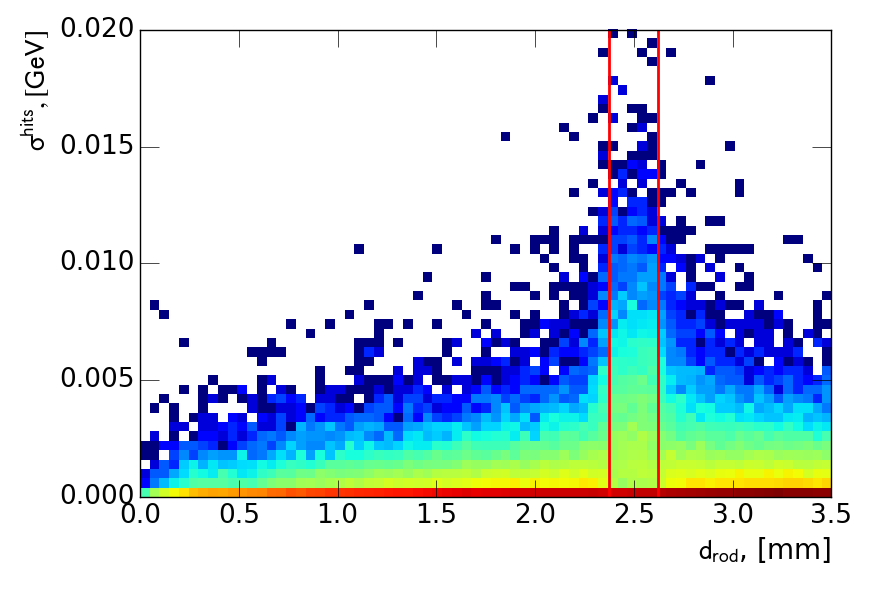
\includegraphics[width=1.0\linewidth]{MC/rms.png} \\ b)}
\end{minipage}
\caption{Distribution of distance to a closest rod center vs a) number of hits in a shower plane and b) standard deviation of hits in a shower energy of electron showers created by electrons with energy less than 1 GeV coming from initial electron with energy 1 TeV. Position of a liquid argon gap is noted by a red lines.}
\label{fig:ShowerProp}
\end{figure}

\begin{figure}[!tbp]
\begin{minipage}[h]{0.49\linewidth}
\center{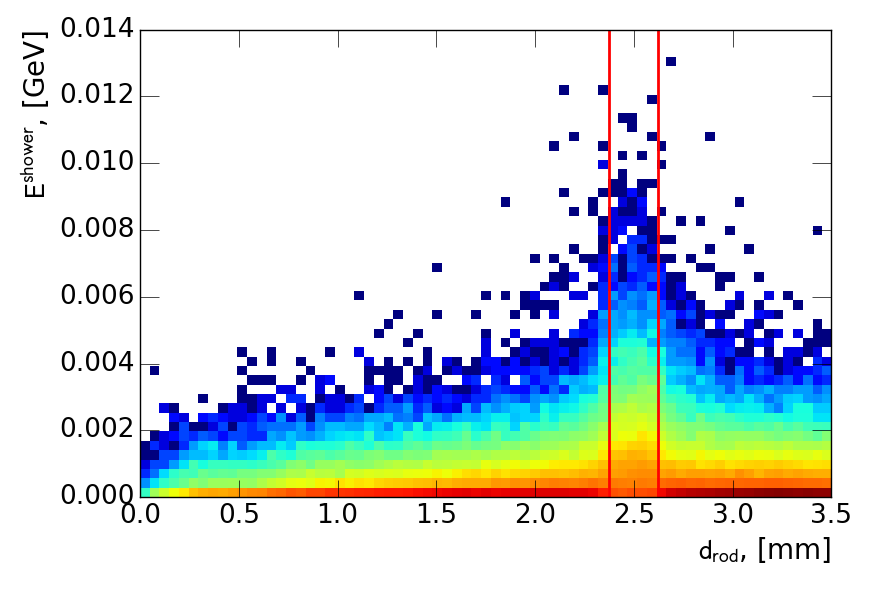
\includegraphics[width=1.\linewidth]{MC/fullBinningScatterSmall.png} \\ a)}
\end{minipage}
\hfill
\begin{minipage}[h]{0.49\linewidth}
\center{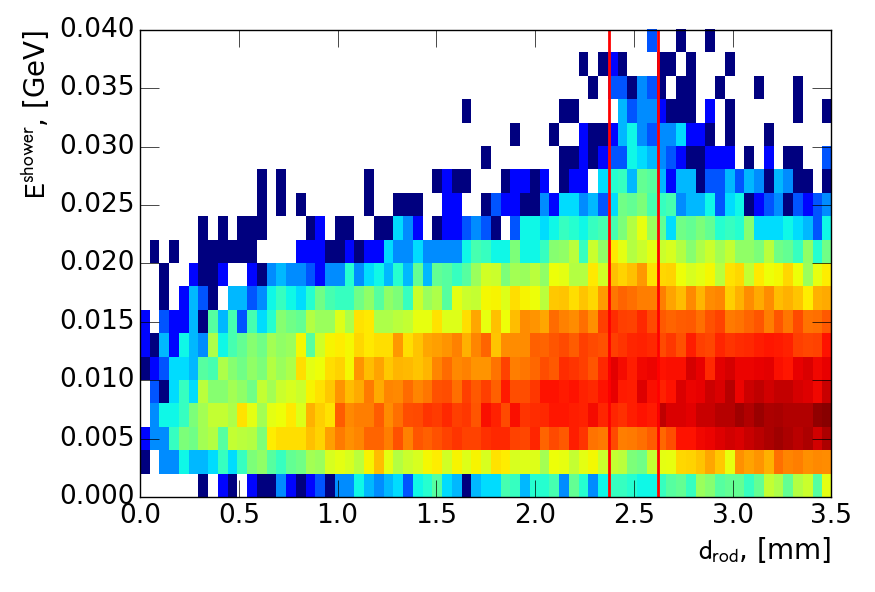
\includegraphics[width=1.\linewidth]{MC/fullBinningScatterBig.png} \\ b)}
\end{minipage}
\caption{Distribution of distance to a closest rod center vs shower energy for electron showers created by electrons with energy a) less than 100 MeV  and b) higher than 300 GeV coming from initial electron with energy 1 TeV in  plane. Position of a liquid argon gap is noted by red lines. }
\label{fig:FSProduction2}
\end{figure}

On the another hand, the use of the frozen showers in too low energy region can be suboptimal because of the small number of energy depositions in a shower. For electrons with energies below 30 MeV 90\% of the showers have no depositions and only 0.5\% of showers have more than 1 hit (Fig.~\ref{fig:fracHits}). It was figured out, that below this energy, the substitution of the electron by the single hit with electron energy have showed a faster speed of simulation.

\begin{figure}[!tbp]
\begin{minipage}[h]{0.49\linewidth}
\center{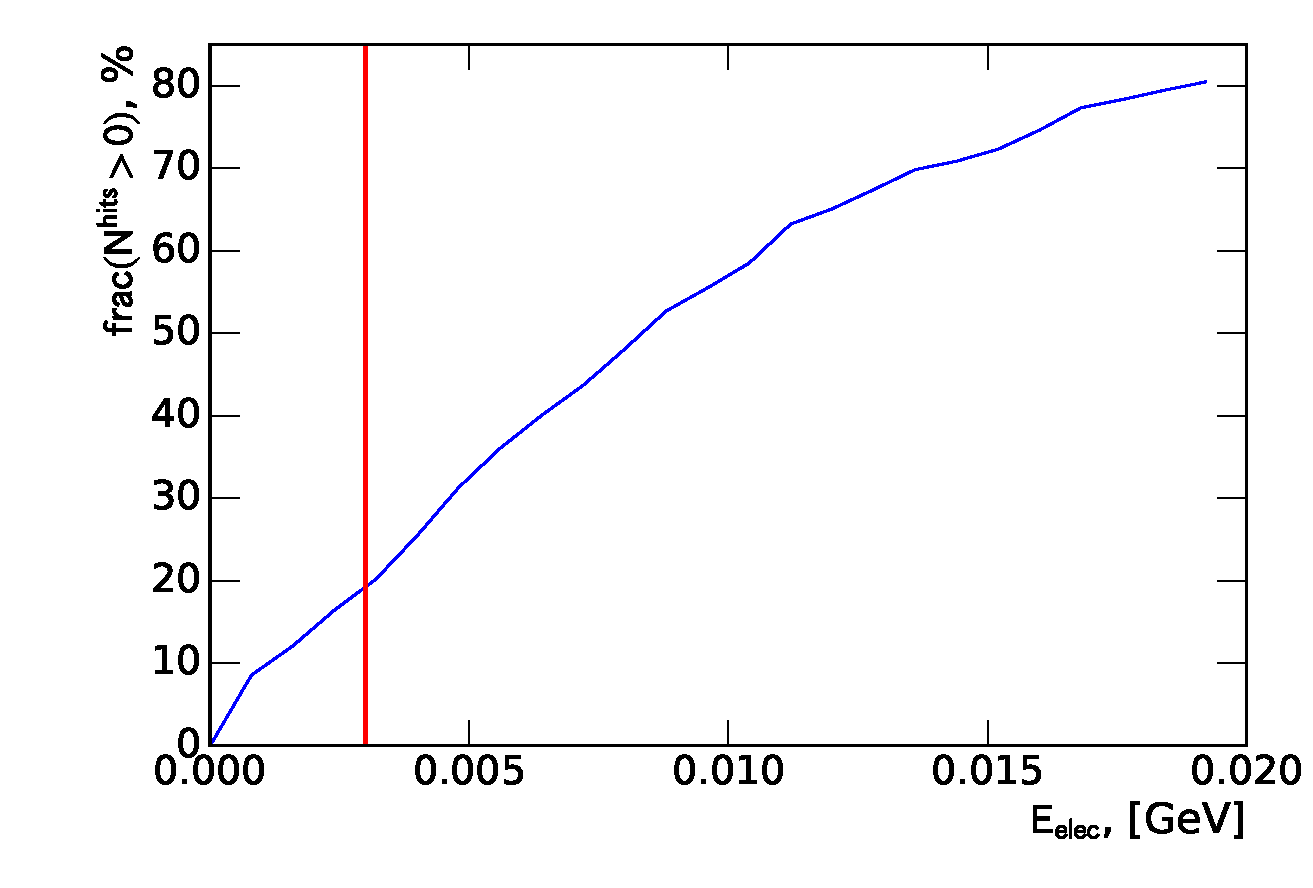
\includegraphics[width=1.\linewidth]{MC/fracHits2.pdf} \\ a)}
\end{minipage}
\hfill
\begin{minipage}[h]{0.49\linewidth}
\center{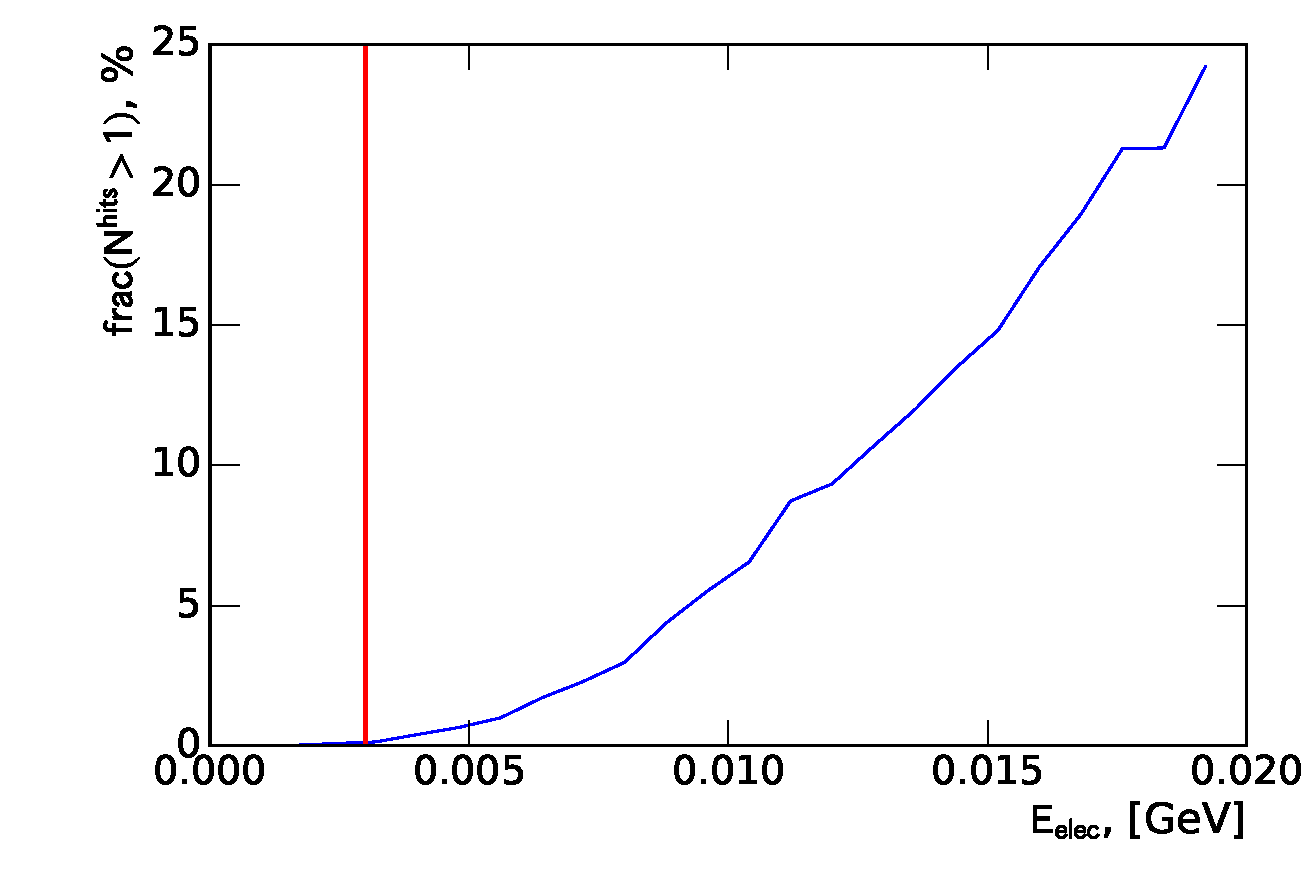
\includegraphics[width=1.\linewidth]{MC/fracHits.pdf} \\ b)}
\end{minipage}
\caption{Fraction of showers with a) at least 1 b) at least 2 depositions inside the sensitive material depending on the initial electron energy. The red line denotes the 30 MeV limit for the frozen showers method.}
\label{fig:fracHits}
\end{figure}


\section{Generation and use in simulation}\label{sec:FSProdUse}

As it was mentioned in the introduction, the frozen showers method consist of two stages: generation of libraries and the use in simulation. The generation needs to be repeated for each significant change in the physics processes description of Geant4 or in the description of the detector. Showers are stored in a library in bins of pseudorapidity and distance to the closest rod center, while the energy remains unbinned. There is special \textit{liquid argon bin} for distance with position and width, that corresponds to the parameters of liquid argon gap, that was introduced in order to catch non-uniformities form Sec.~\ref{sec:FSproblem}.

In order to obtain a proper energy distribution for the generation of the library, particles originating from SM process ($t\bar{t}$ or high energy electrons) are usually used. For each particle eligible for frozen showers use parameters are saved for a later use. On a second stage, these particles are propagated through the calorimeter using full \atlas simulation infrastructure. Each hit is saved as a shower inside the library in a corresponding pseudorapidity and distance bin. 

Additionally, in order to save disk space as well as a memory consumption, the hit information is compressed. This compression is performed in two steps: 
\begin{description}
\item [Hit merging] If the distance between any two hits is smaller, than a given parameter $R_{min}$, then these hits are merged into one deposit at the energy weighted center of them. This process is done iterativelly.
\item [Truncation] Hits which energies are below a fixed fraction $f$ of the total energy sum of all hits, are truncated. The energy of the remaining hits is rescaled in order to preserve the total deposited energy.
\end{description}

During simulation, if the energy of a particle falls below a cut-off energy, the FS algorithm examines the resulting shower. It checks whether the particle is far from the edges of the calorimeter, such that the  shower is by 90\% contained inside the calorimeter. This depends also on the energy of the particle, since the  shower sizes are increasingly growing with energy. The algorithm searches for a shower with the closest energy in the corresponding pseudorapidity and distance bins. The shower is rotated in the direction of the particle. In order to correct for the differences in the energy, each hit in the shower is scaled as:
\begin{equation}
E_{hit}^{new}=E_{hit}\cdot \frac{E_{part}}{E_{part,lib}},
\end{equation}
where $E_{hit}$ is the original energy of the hit, $E_{part}$ is the energy of the particle and $E_{part,lib}$ is the energy of the particle from the library. Afterwards particle is substituted by the resulting shower. Later, the reconstruction algorithm uses these hits from the frozen shower as usual energy deposits in the sensitive material. 

\begin{figure}[!tbp]
\center{
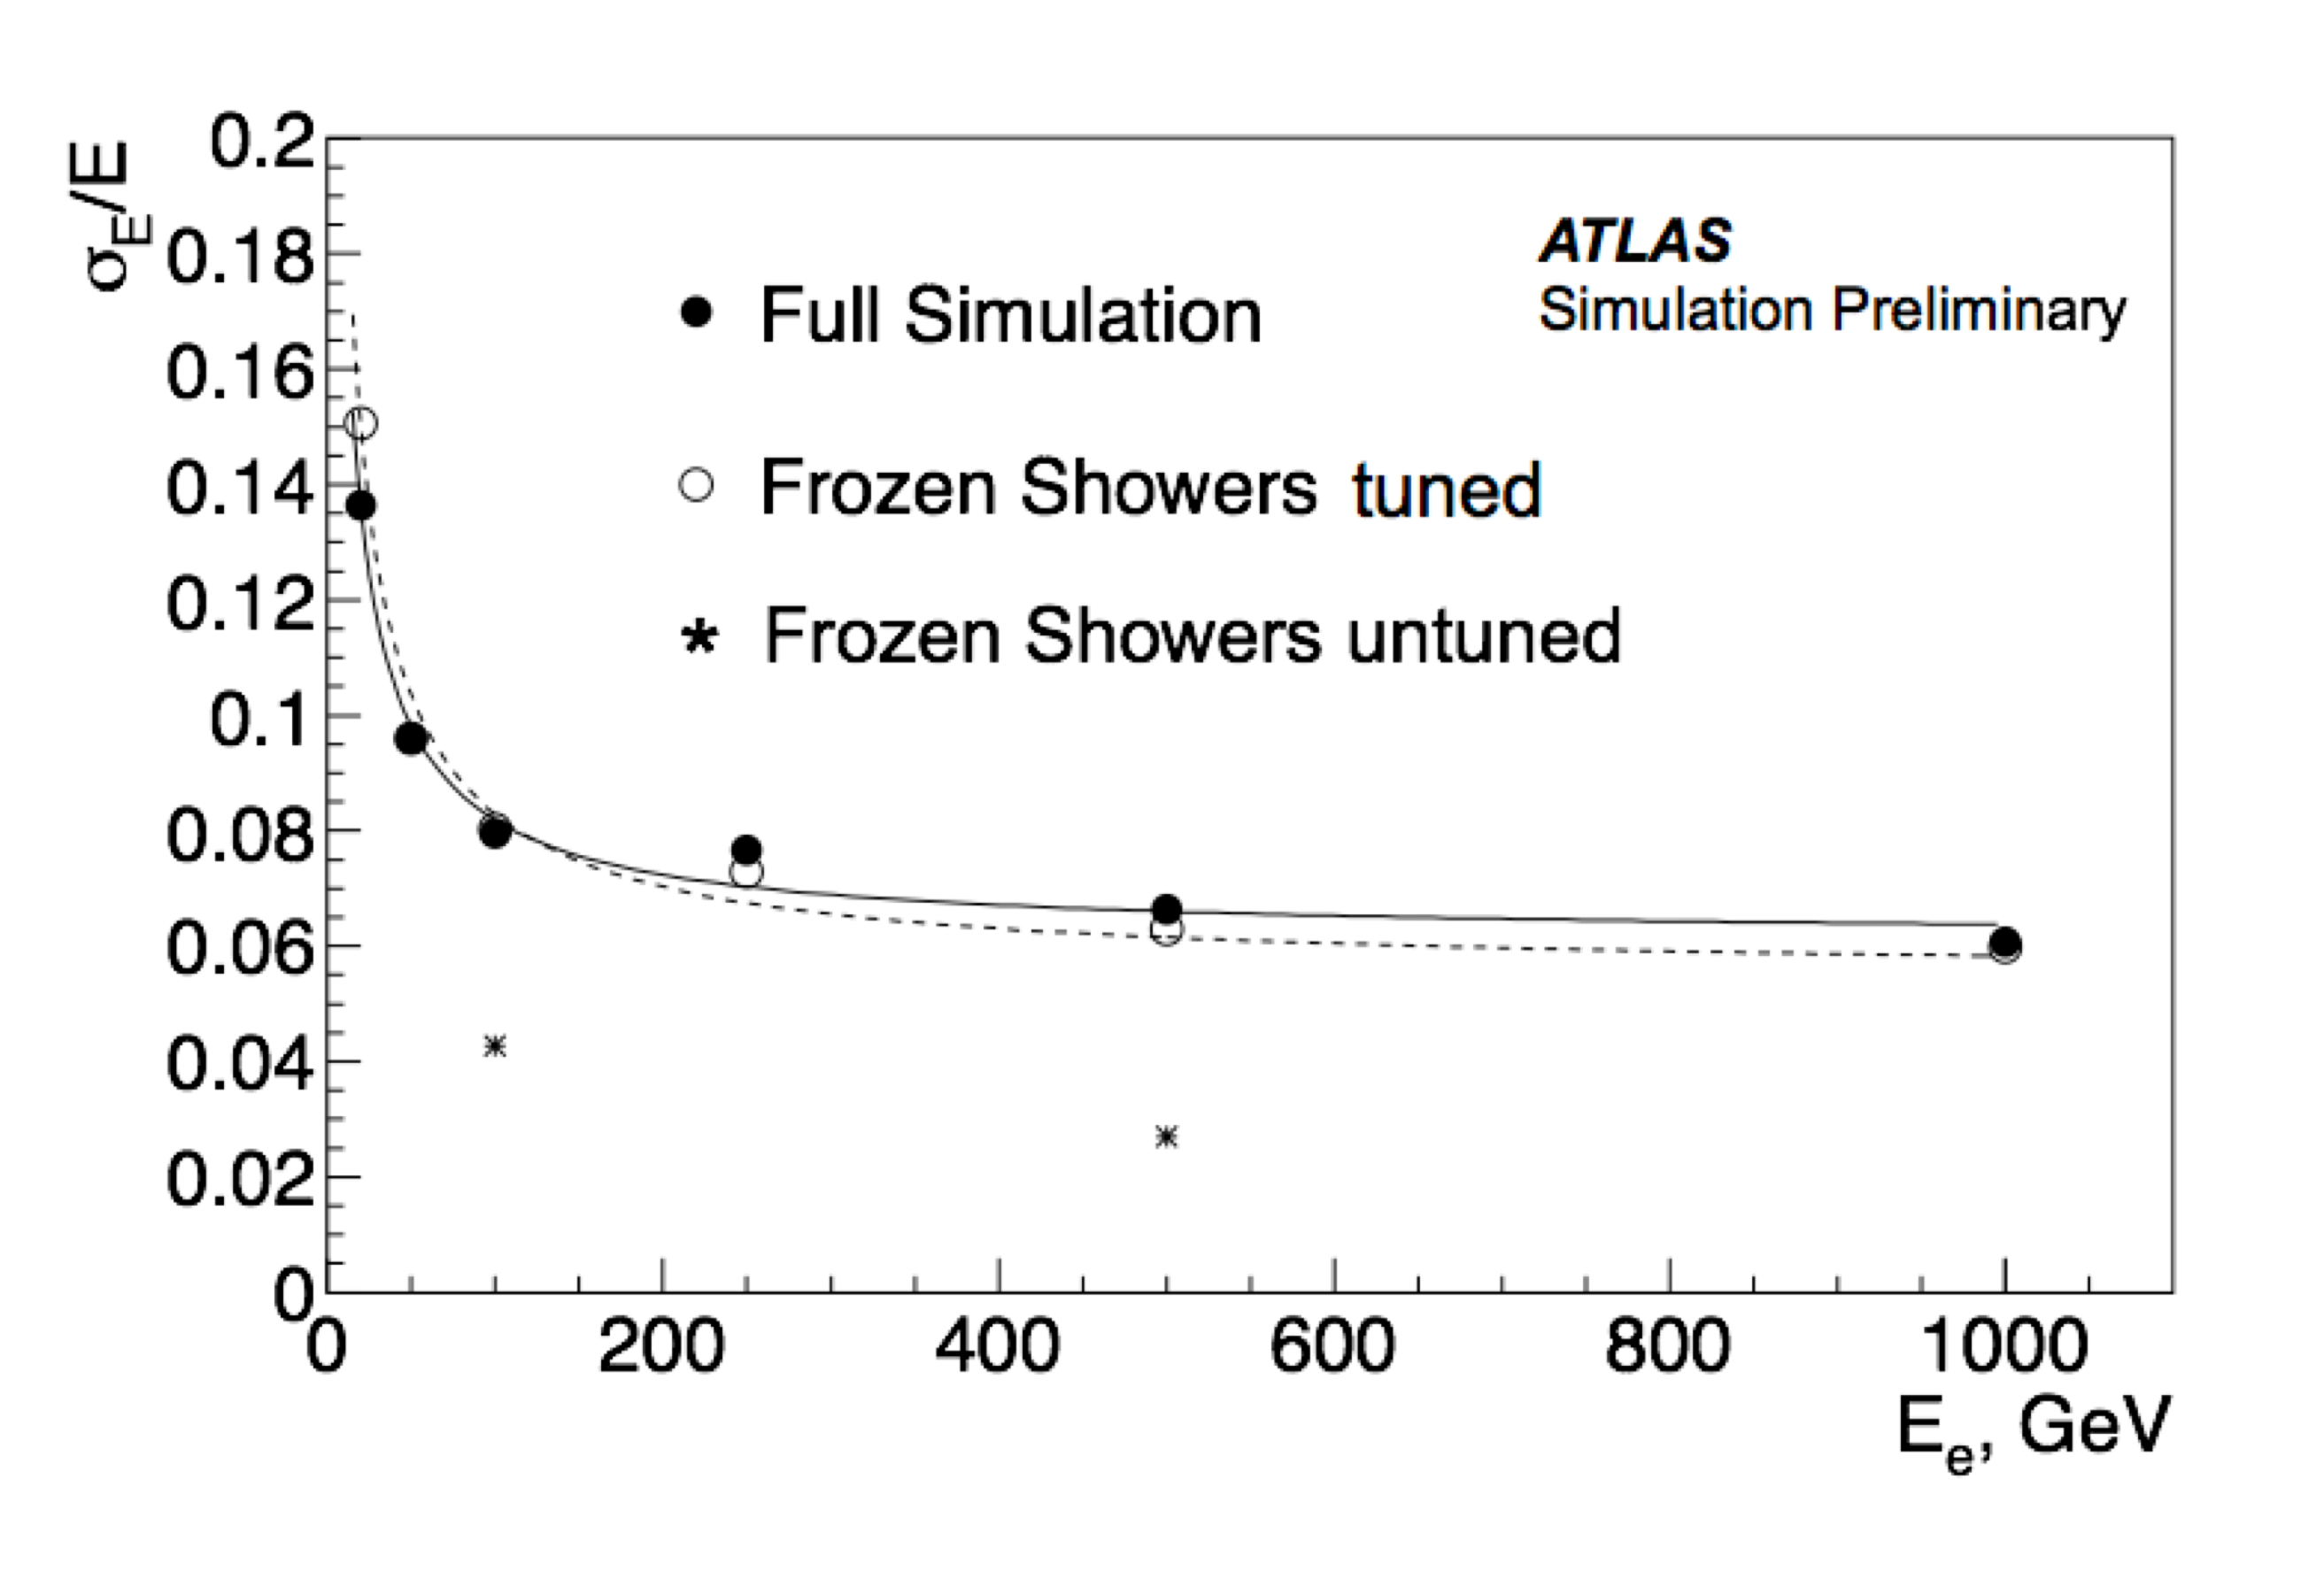
\includegraphics[width=0.8\textwidth]{MC/fs.png}
\caption{Electron resolutions for full simulation(black dots), tuned(white circles) and untuned(star points) frozen showers. Electrons simulated with frozen showers libraries before tuning have twice smaller resolution, than electrons from full simulation. Tuning allows to gain better agreement with full simulation.}
\label{fig:FS_resolution}}
\end{figure}

\begin{figure}[!tbp]
\center{
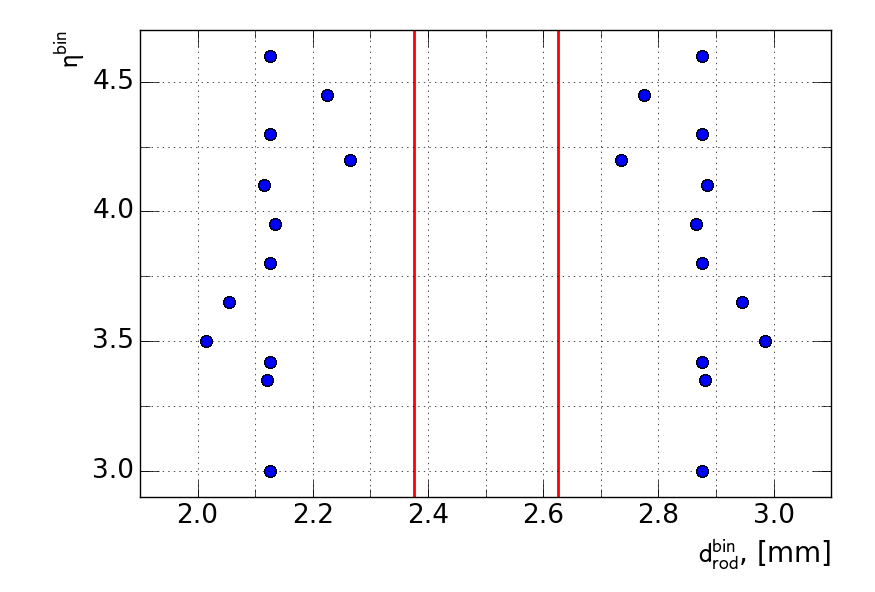
\includegraphics[width=0.8\textwidth]{MC/oldTuning.png}
\caption{Position of gap bins for different $\eta$ bins in the previous libraries after tuning. The dots correspond to the limits of each bin. The red lines are denoting the original position of the bins, which correspond to the position of the liquid argon gap in the calorimeter.}
\label{fig:FSOldTuning}}
\end{figure}

\subsection{Tuning of libraries-}\label{sec:LibTuning}

The good simulation method is required to be consistent with full simulation on all possible reconstucted objects. In case of Frozen Showers in forward calorimeter, the electron energy resolution is the most problematic value, since the resolution of the reconstructed electrons is around 2 times smaller(Fig.~\ref{fig:FS_resolution}), than in the full simulation. Using the Eq.~\ref{eq:EMResoultion}, this behavior can be interpreted as a smaller size of fluctuations for fast simulation and therefore lack of the high-energy showers originating in sensitive matrial. This problem can be solved by tuning the parameters of library in order to match the full simulation.

The tuning consists of a 2-step manual procedure:
\begin{description}
\item [Changing bin width] At this stage position of the liquid argon bin is moved, so what a bid width is enlarged. This causes a higher number of showers with higher response in simulation and therefore higher fluctuations. This procedure causes a higher resolution and a mean energy of reconstructed electrons.
\item [Shower energy scaling] In order to correct for the introduced shift in the energy scale, the shower energy is reduced by rescaling all the hits in the shower to the shift in the mean reconstructed energy.
\end{description}
 It is repeated iterativelly in each pseudorapidity bin separately untill the desired agreement is obtained. The resulting bin positions are shown on a Fig.~\ref{fig:FSOldTuning}. This method yields a relatively good agreement with full simulation (black dots on Fig.~\ref{fig:FS_resolution}). However, it is necessary to repeat this procedure for each new library generation and this requires a significant tuning effort, which makes it not optimal. 

\section{Machine learning based bin finding procedure}\label{sec:MLBinning}

Since frozen showers were planned to be used in the Run-2 Monte Carlo production, there was a need for a more automatic procedure of library generation with proper electron resolution. One of the possible ways is to choose the different positions of liquid argon bins during library generation using machine learning tools. In this section a newly developed automatic bin finding procedure will be discussed.

\subsection{Machine learning introduction} 

Machine learning is a set of algorithms, which allows algorithms to learn and improve from experience without being explicitly programmed. This is a modern field of computer science, that is used in different fields like computer vision, natural language processing, data science etc. There are two main types of machine learning algorithms: \textit{supervised}, where a example of the desired output is provided by the "supervisor" and the goal is to learn a general rule, that maps inputs to outputs, and \textit{unsupervised} learning, where no labels are given to the algorithm, which discovers the hidden patterns in the data\cite{0070428077}. The initial data parameters of interest, which are used in the algorithm to "learn" are called \textit{features}. 

Machine learning algorithms can be used for solving a classification problem, where each event should be identified to one of the specified classes. Since the first introduction of machine learning classifying algorithms called perceptron by Rosenblatt\cite{VanDerMalsburg1986}, many different algorithms have been invented. In this analysis, decision trees and support vector machines implemented in Scikit-Learn python package\cite{scikit-learn} are used. 

\subsubsection{Binary decision trees}

\textit{Binary decision trees}\cite{cart84-2}, called also single decision trees, are one of the most commonly used machine learning algorithms for a classification problems in particle physics. It can be represented as a set of sequential cuts on input variables. 
Scheme of this algorithm is shown in Fig.~\ref{fig:MLAlgo} a). Red circles show the nodes of the tree. Each node corresponds to the one of the internal input variables and connects to two branches, that are split in the respect to the value. The first node is called a root node. The depth of the tree is the number of branches from the node to the tree's root node. The tree ends with squares, called leaf nodes, where all events are classified to a certain class. Leaf node represents classification or decision. The tree, where each node has at most 2 children called binary decision tree.

The tree is build using the variable called Shannon entropy\cite{ShannonEntropy}, what is similar to the entropy in physics:
\begin{equation}
S=- \sum_{i=1}^{N} p_i log_2 p_i,
\end{equation}
where $p_i$ is the probability to find event of class i. Each split in a variable should decrease the entropy of the system. The information gain is defined as the difference in entropy after the split:
\begin{equation}
IG(Q) = S_0 - \sum_{i=1}^{2}S_i,
\end{equation}
where $S_0$ is the initial entropy, without new node, $S_i$ is the entropy of the one of the 2 node children. The node with the highest information gain is taken. One of the main advantages of the decision trees its simplicity of visualization and interpretation. 

\subsubsection{Support vector machines}

\begin{figure}[!tbp]
\begin{minipage}[h]{0.49\linewidth}
\center{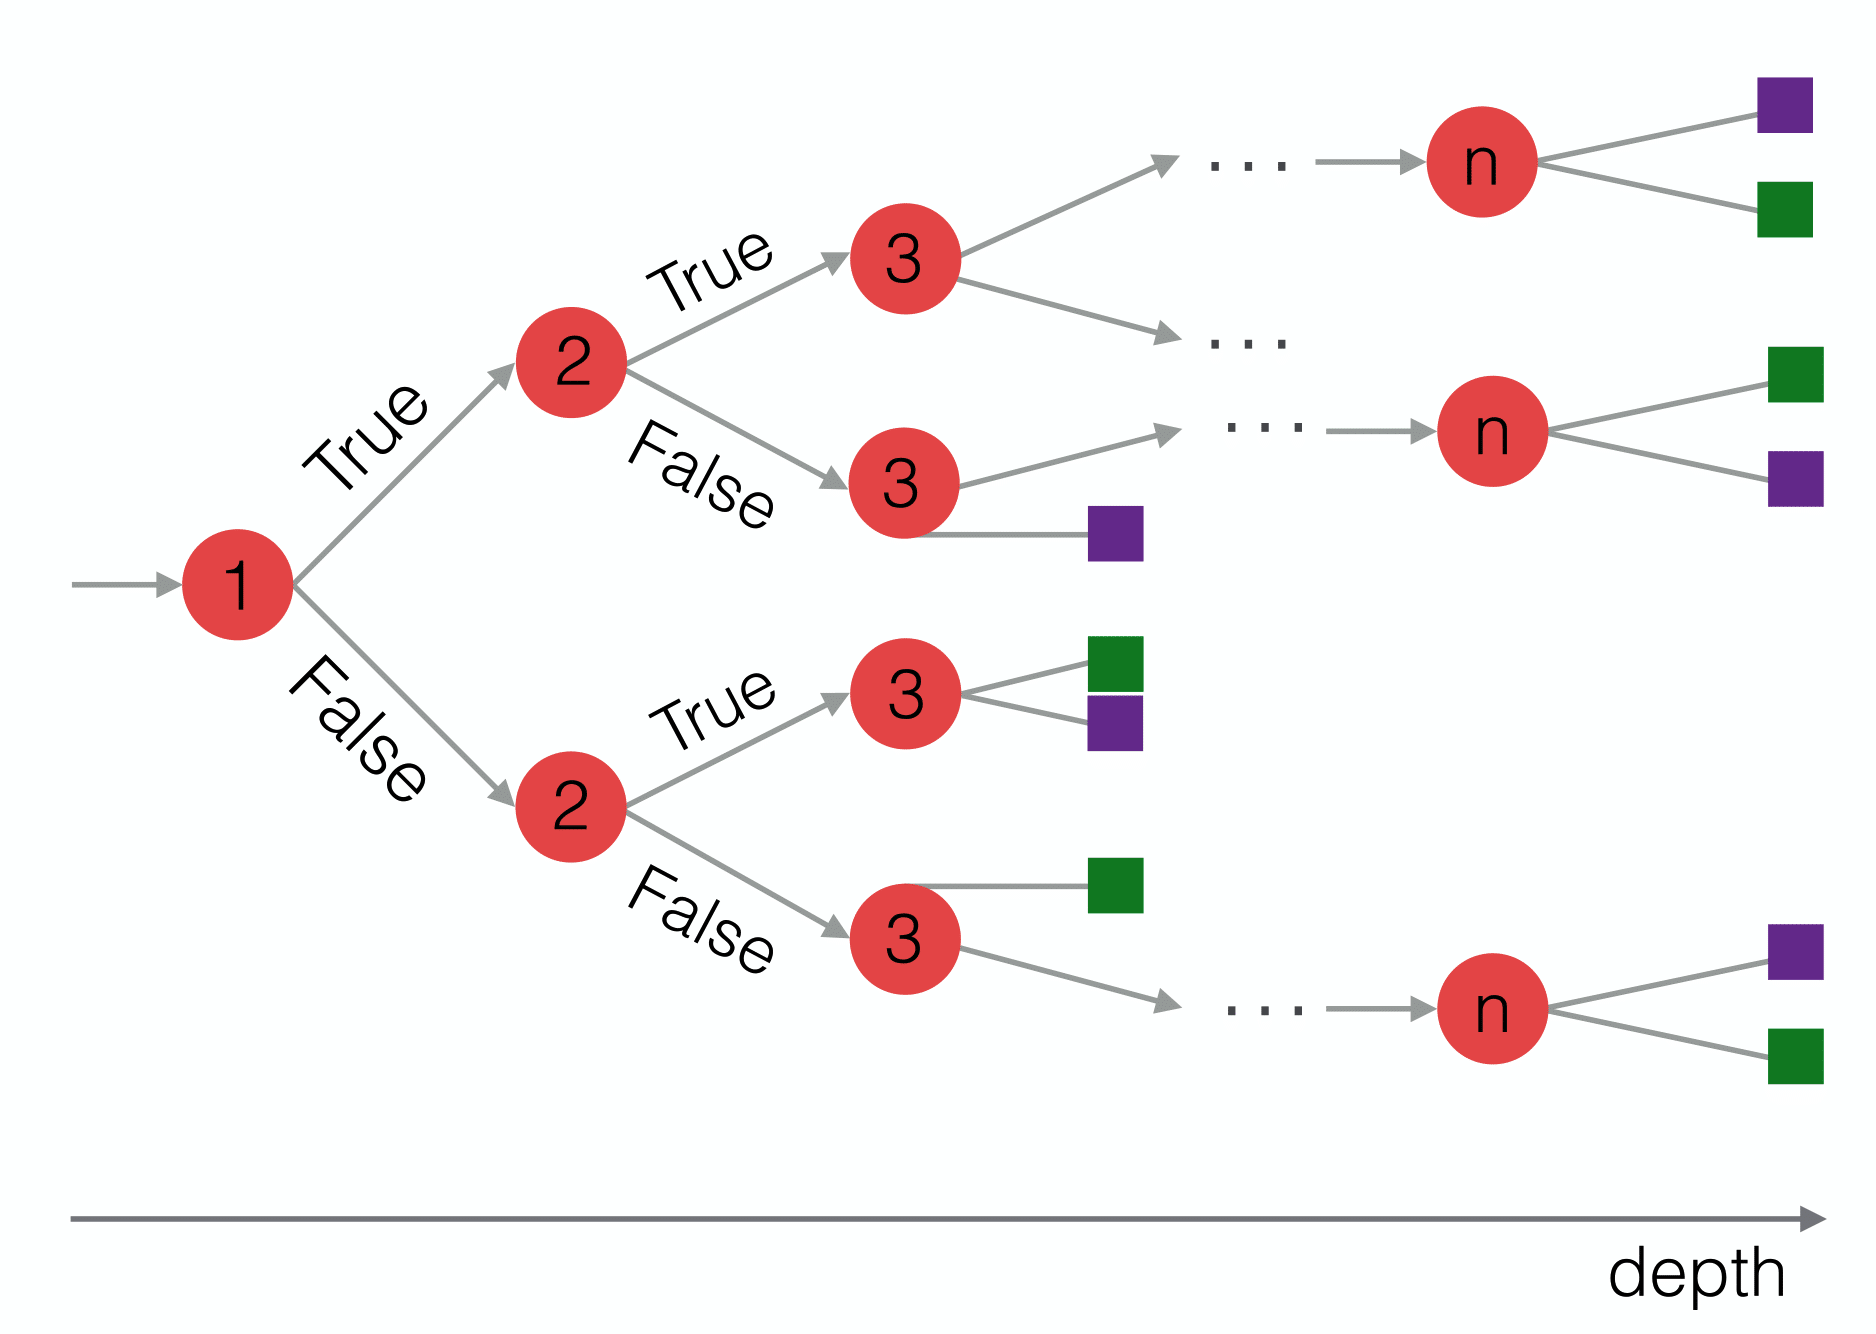
\includegraphics[width=1.\linewidth]{MC/DecisionTree.png} \\ a)}
\end{minipage}
\hfill
\begin{minipage}[h]{0.49\linewidth}
\center{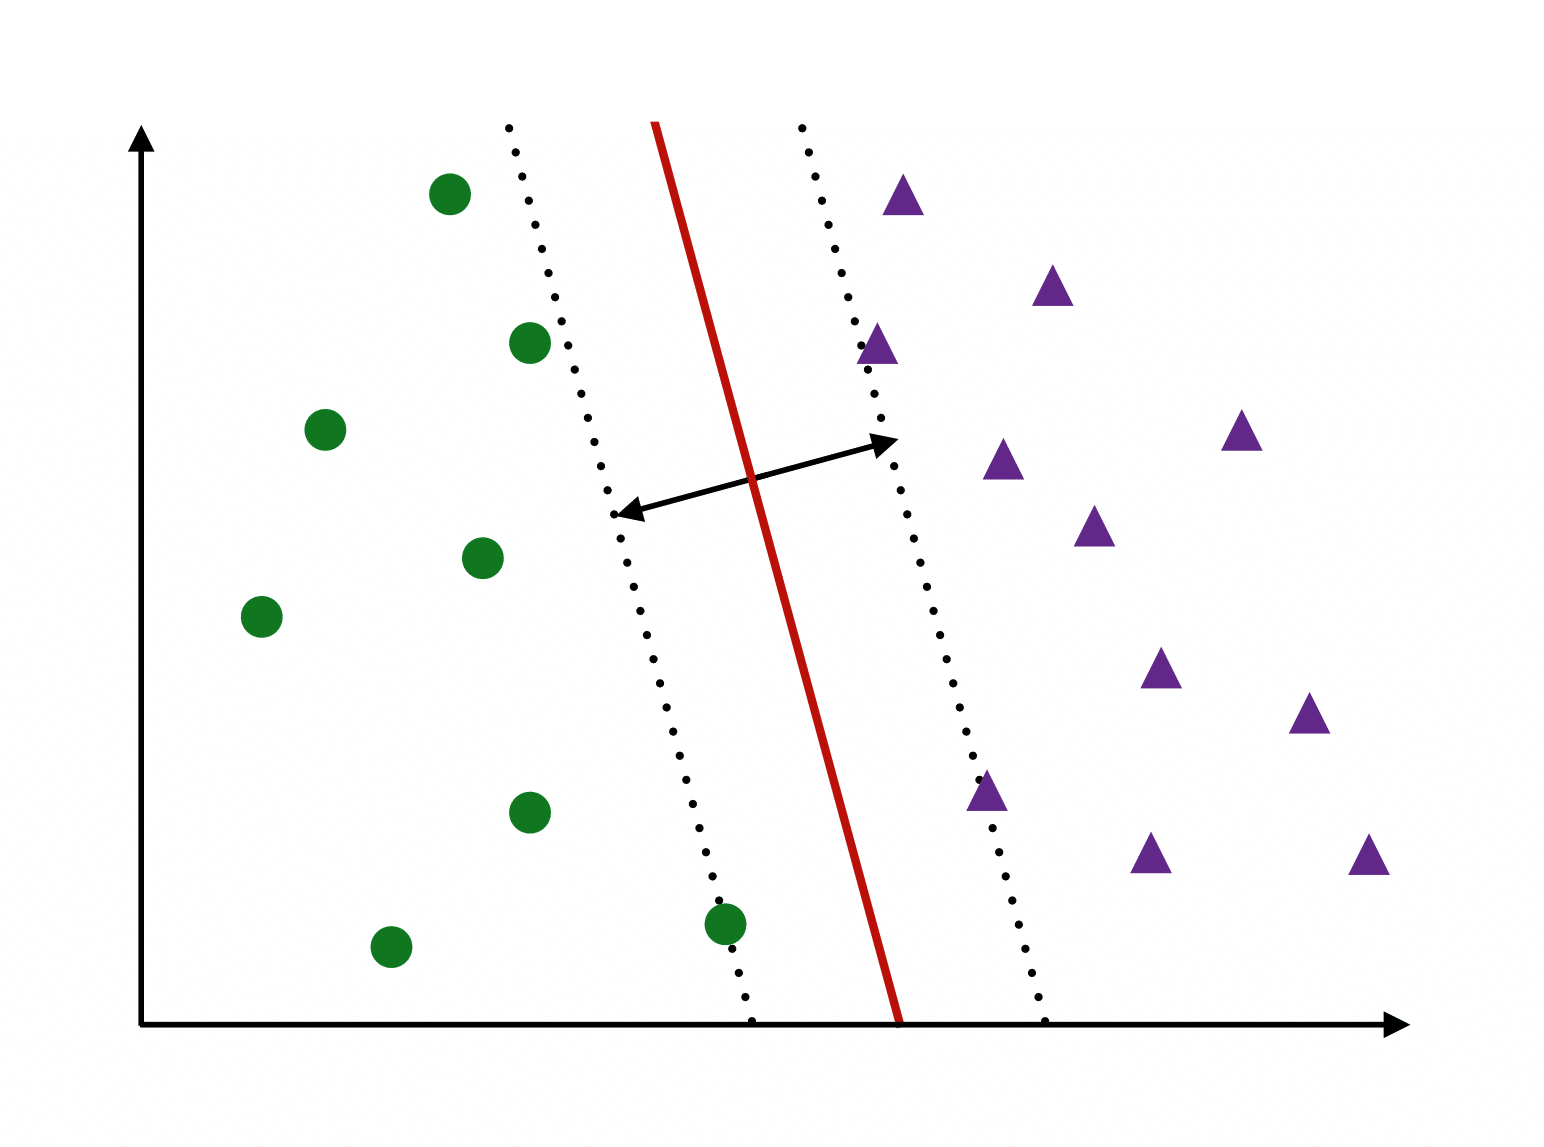
\includegraphics[width=1.\linewidth]{MC/SVM.png} \\ b)}
\end{minipage}
\caption{Schematic representation of machine learning algorithms, used in this analysis for the classification of showers. Green figures represent the first class of events, whereas violet ones belong to a second class.  
a) Representation of a binary decision tree structure: red circles correspond to nodes, which are split with the respect to the selected feature. Squares represent leafs, where events classified to a certain class. The depth of the tree is calculated as a maximum number of edges from the node or leaf to the root node. 
b) Representation of the SVM algorithm. The dividing hyperplane is shown by the solid line. The dashed lines represent the maximum margin boundaries.}
\label{fig:MLAlgo}
\end{figure}

\textit{Support vector machines} (SVM) is a supervised machine learning algorithm which can be used for classification problems\cite{VapLer63}. In this algorithm each event is represented in a p-dimensional parameter space. The classification is performed by finding hyper-plane that differentiates given two classes with the largest possible separation (Fig. ~\ref{fig:MLAlgo} b). The hyperplane can be described with the set of points $\vec {x}$ in the parameter space satisfying:
\begin{equation}
\vec{w}\cdot \vec{x} - b = 0,
\end{equation}
where $\vec{w}$ is the normal vector to the hyperplane and the parameter $\frac {b}{\|{\vec {w}}\|}$ determines the offset of the hyperplane from the origin along the normal vector $\vec {w}$. 

The maximum margin boundaries are described by equations:
\begin{eqnarray}
\vec{w}\cdot \vec{x} - b = 1, \\
\vec{w}\cdot \vec{x} - b = -1,
\end{eqnarray}
where $\frac{2}{\|\vec{w}\|}$ is the distance between these 2 hyperplanes, such that the planes with the maximum margin between them should have  minimum $\|\vec{w}\|$. 

In order to prevent each point from falling into the margin, the following constrain should be satisfied: 
\begin{eqnarray}
\vec{w}\cdot \vec{x} - b \geqslant 1 \textrm{ where } y_i = 1,\\
\vec{w}\cdot \vec{x} - b \leqslant -1 \textrm{ where } y_i = -1,
\end{eqnarray}
where $y_i$ represents the class of the i-th event, that can be either 1 or -1. These equations can be rewritten as:
\begin{equation}
y_i(\vec{w}\cdot \vec{x} - b ) \geqslant 1
\end{equation}

It is also possible to construct a non-linear classifier by replacing the dot-product with a different kernel function. In this thesis, a radial basis function (RBF) kernel is used:
\begin{equation}\label{eq:RBF}
K_{rbf}(\vec{x}_i, \vec{x}_j) = e^{-\gamma | \vec{x}_i - \vec{x}_j|^2} \, \gamma >0,
\end{equation}
where the parameter $\gamma$ adjusts the width of the kernel.




\subsection{Electron shower categorization}

\begin{figure}[!tbp]
\center{
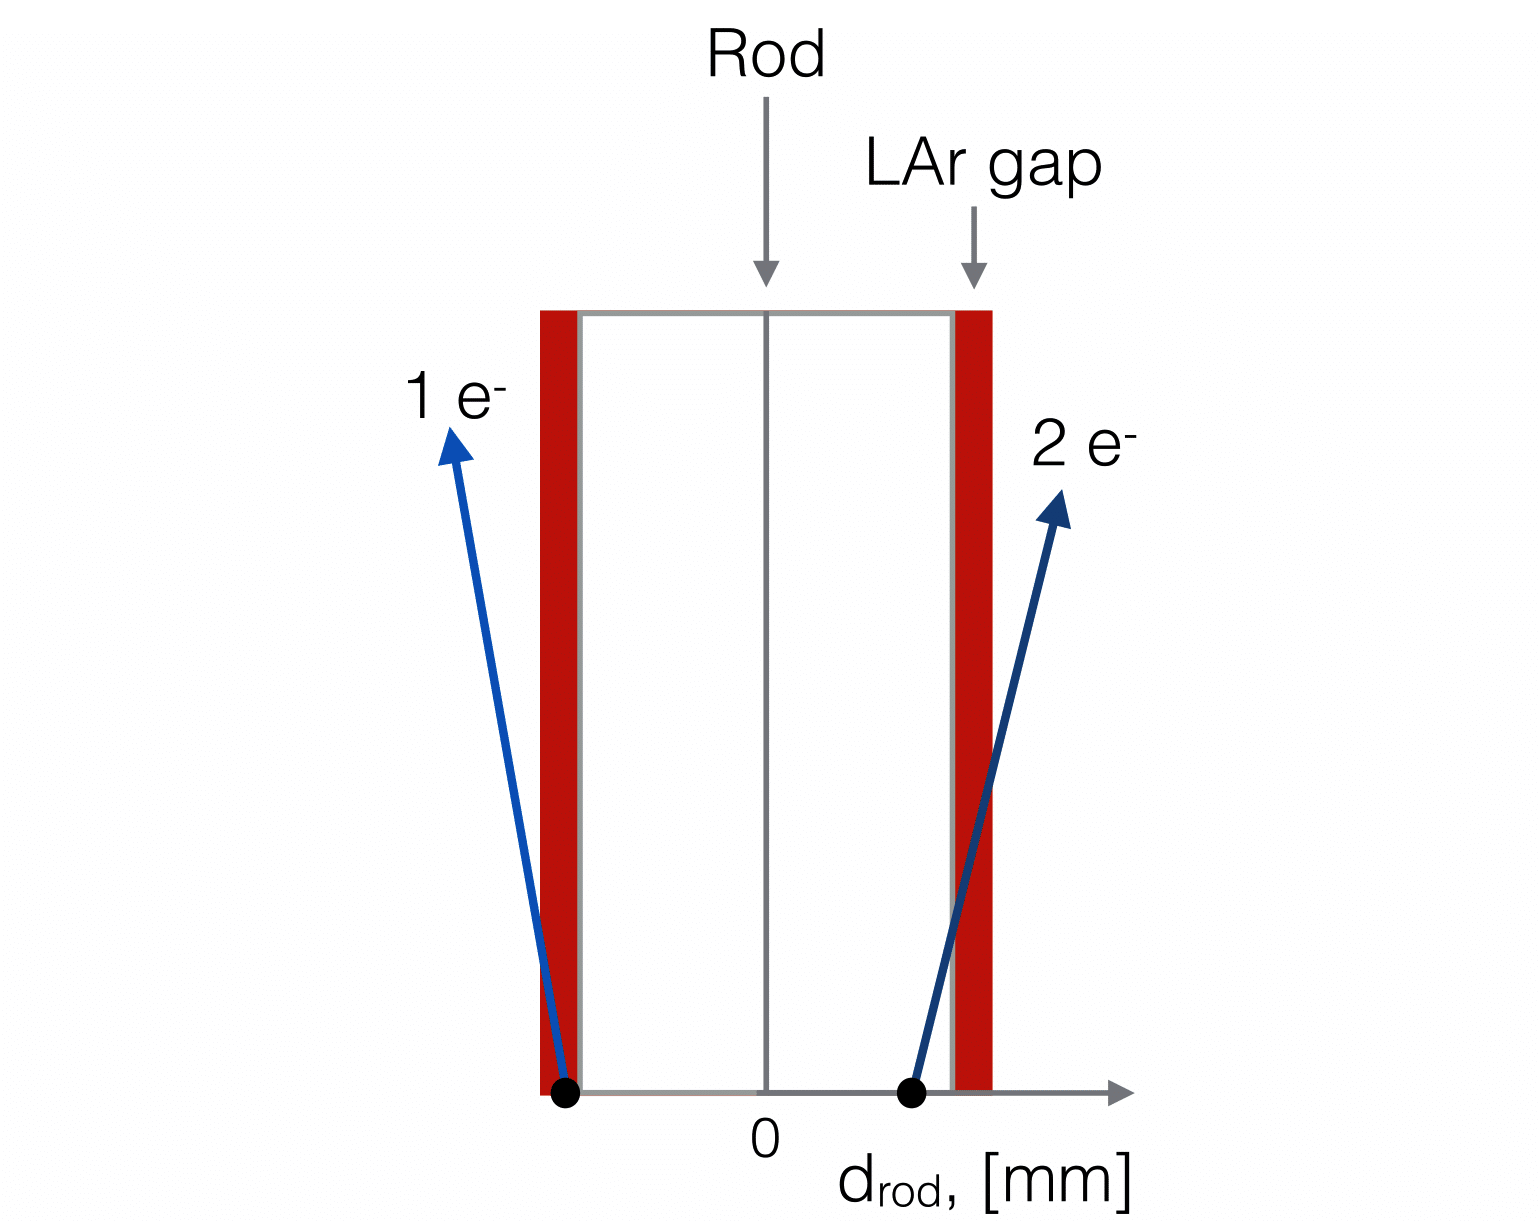
\includegraphics[width=0.5\textwidth]{MC/Model2.png}
\caption{Schematic representation of the model of shower creation in the FCAL. Electron 1 is created in a liquid argon gap. Electron 2 is created near a liquid argon gap and crosses it. This causes a smearing of sensitive material showers distribution. Electrons created in the sensitive material tend to create more energetic showers, than electrons from the dead material. However, electrons shown on this scheme may give similar showers and therefore may not be distinguishable.}
\label{fig:Model}}
\end{figure}

As it was mentioned in the previous sections, the FCAL modules consist of different types of material such that showers starting inside the dead material are usually having lower energies, than those started in sensitive material. However, the validation (Fig.~\ref{fig:FS_resolution}) can be interpreted as an implication that there are high-energy showers outside the liquid argon gap. It could be explained by the fact, that electrons, created in a dead material, can cross a liquid argon gap and give a hit there as shown in Fig.~\ref{fig:Model} (electron 2). These electrons would be indistinguishable from electrons created directly in the sensitive material (electron 1 in Fig. \ref{fig:Model}). 

Due to this similarity, electrons created outside the sensitive material can be treated together, labelling such showers \textit{sensitive matrial showers}. Showers that did not cross a liquid argon gap, are called dead material showers. This means, that in this model a real liquid argon gap can be substituted by the "effective" one, with larger width.

The width of the effective liquid argon gap, from the definition, depends on the following parameters:
\begin{description}

\item [Electron energy] The gap should get wider with higher energy of the initial electron, because of the growth of the mean free path with energy.
\item [Direction of the electron] Electrons aligned collinearly with the liquid argon gap will have smaller probability to cross it. This probability will grow with the angle reaching its maximum at  $90^{\circ}$

\end{description}

The bin finding is performed as a 2-step procedure:  on the first stage the first classifier distinguish the showers based on their simulated parameters and on the second step the second classifier aims to produce a hyperplane in $d_{rod}$, $E$ of initial electron phase-space. This classifiers and the training sample used will be discussed in details in the following subsections.

\subsubsection{Training sample}

Real distributions of parameters of electrons, used in simulation, have a complicated structure and depend on the physics processes simulated. Machine learning could identify these dependencies instead of the needed ones. This is why a simplified data is needed as a training sample for machine learning. The training sample was produced by simulation of electrons directly in the forward calorimeters. In order to treat equally high and low energy electron initial showers, a uniform energy distribution is used.

Fig.~\ref{fig:EtaMomVsEnergy} shows the distribution of the shower direction ($\eta^{direction}$) vs electron energy for electrons coming from simulation of 1 TeV electron. Most of the showers have direction in $\eta$ range between 3.0 and 5.0, which corresponds to position of the FCAL. It was figured out, that the direction of the shower is highly correlated with the postion of the electron. Therefore, electrons were generated uniformly in $\eta$ between 3.0 and 5.0.


\begin{figure}[!tbp]
\center{
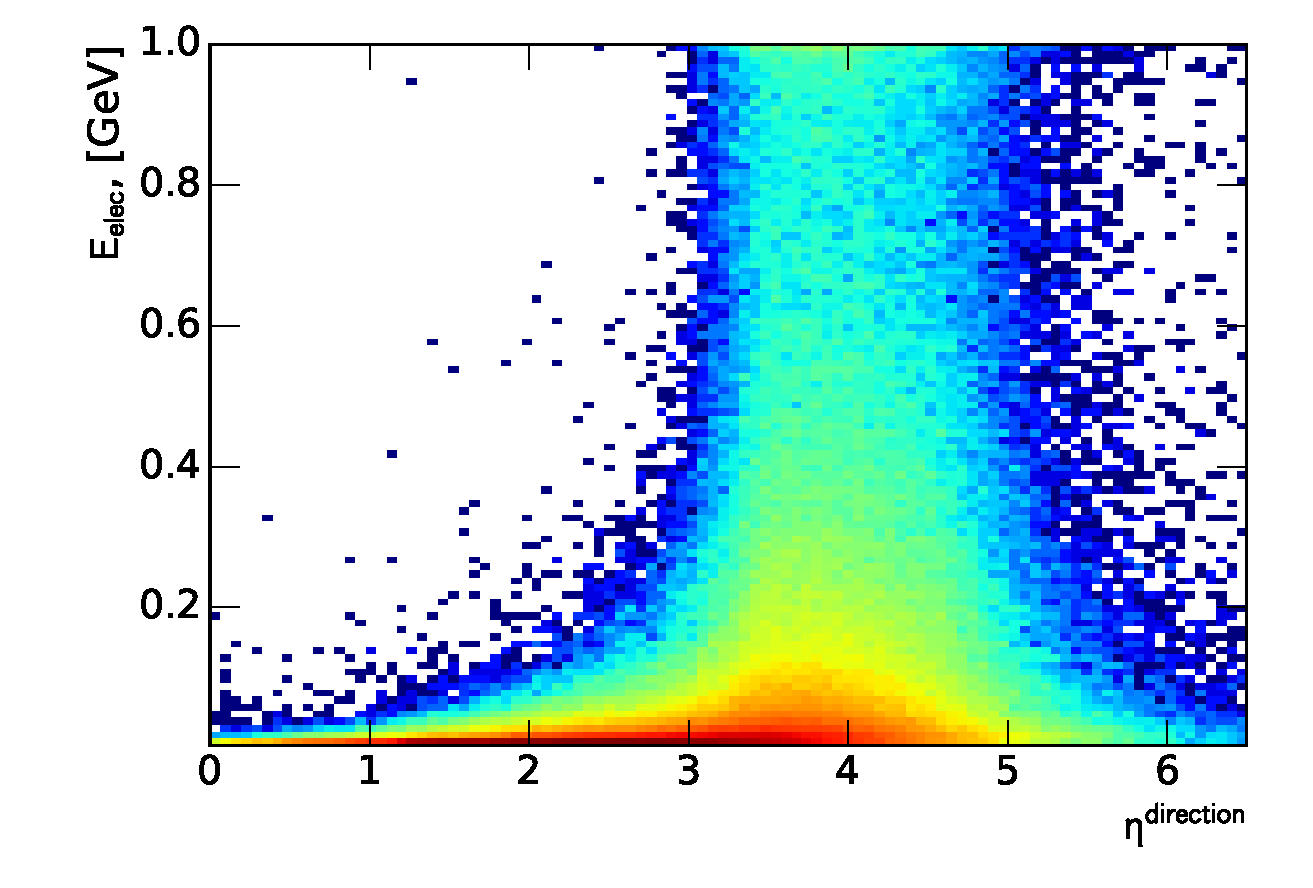
\includegraphics[width=0.8\textwidth]{MC/FSEtaMomVsEnergy.pdf}
\caption{Distribution of sub-showers energy vs direction of shower $\eta_{momentum}$ for showers from the production of 1000 GeV electrons.}
\label{fig:EtaMomVsEnergy}}
\end{figure}

\subsubsection{First classifier}

The first classifier aims to categorize all showers by means their parameters. An supervised learning algorithm is used on artificially reduced training sample, where the labels can be put automatically. The obtained classifier is later expand the classification to the full training sample. 

Pre-labeling is done using the definitions of sensitive and dead material showers based on the distance to a closest rod center (Fig.~\ref{fig:SchemePresel}). Showers starting in a liquid argon gap are defined as sensitive material showers, while showers coming from electrons born near the rod center and on the edges of the cells can be labeled as dead material showers, since there is a small probability for the electron, which caused the shower, to reach the liquid argon gap.

For this classifier a simple decision trees have been chosen, since it has showed a good classification efficiency on the reduced training sample. Different input parameters have been tested using their variance, and it was figured out, that the best set of the differentiating parameters is:

\begin{itemize}
\item Shower energy, defined as the sum of all sensitive material hits energies in the shower;
\item Maximum hit fraction. This quantity is calculated as the energy of the most energetic hit divided by the shower energy;
\item RMS of the hits, calculated as the standard deviation of the hits energies in the shower.
\end{itemize}

The classification efficiency of the obtained binary search tree on the reduced sample with the depth = 2 is 97\%. The expanded to the full phase-space results are shown in Fig.~\ref{fig:Class} a). 

\begin{figure}[!tbp]
\center{
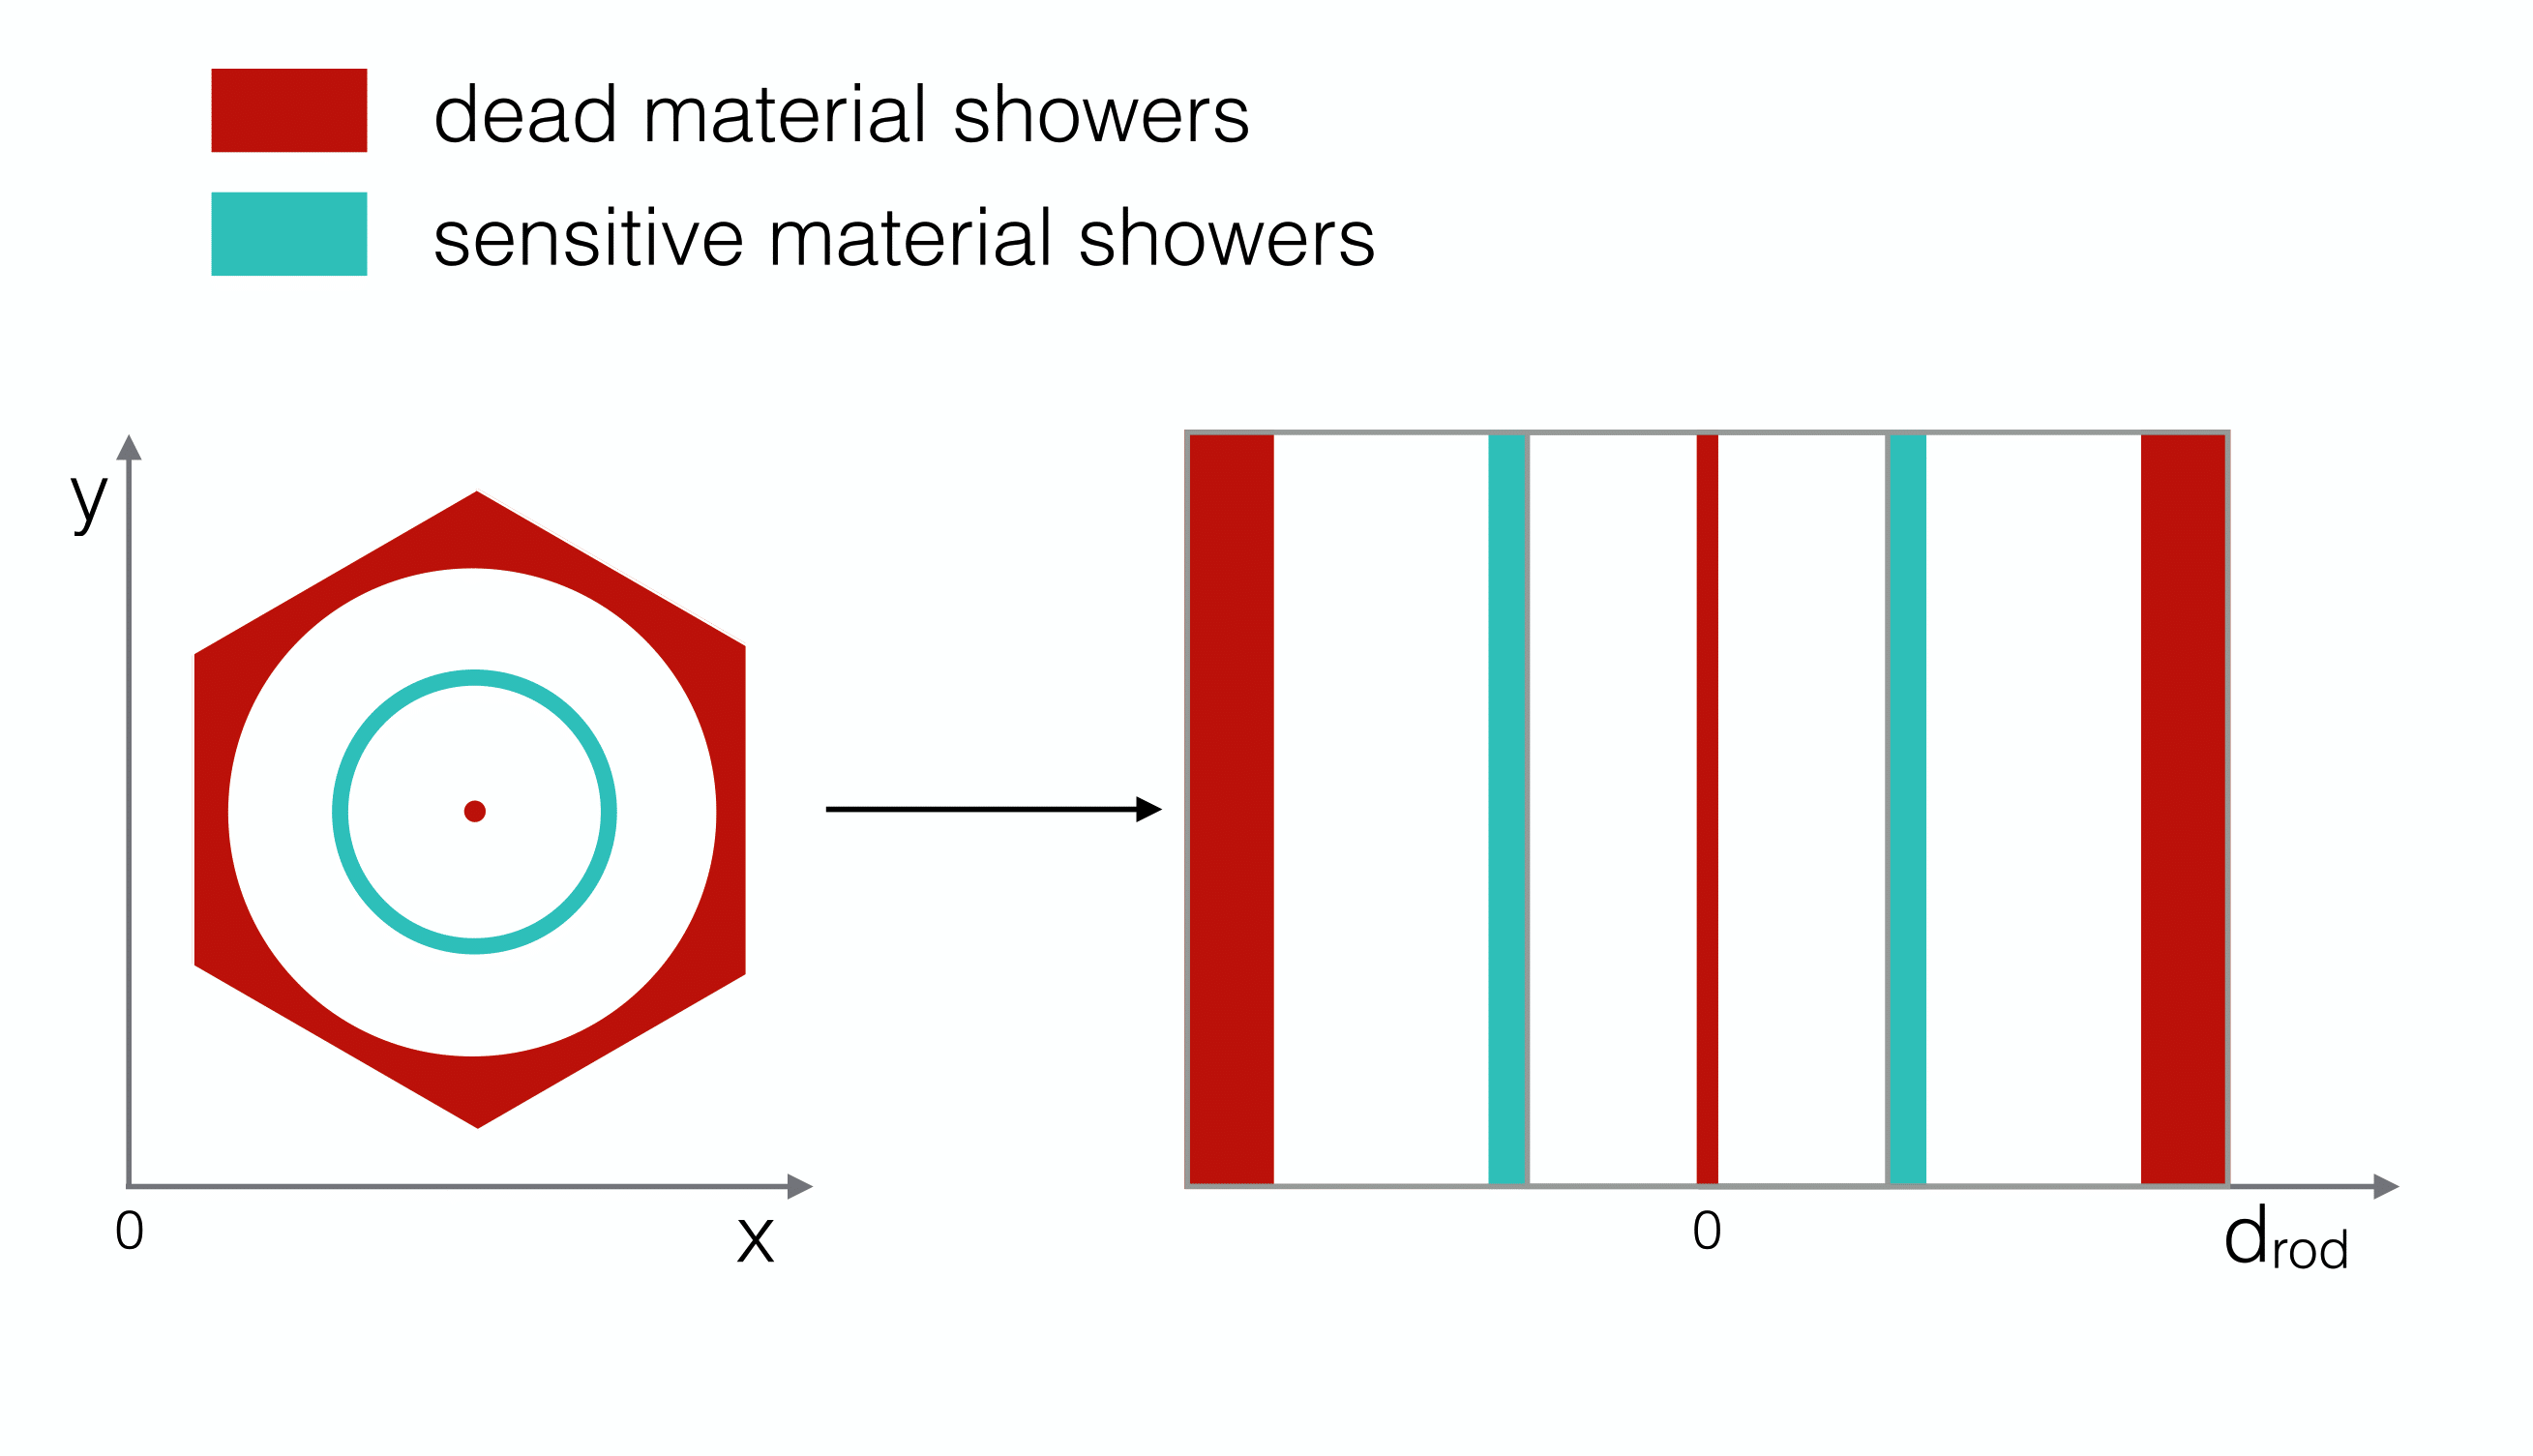
\includegraphics[width=1.0\textwidth]{MC/FirstClassifierData.png}
\caption{Schematic representation of the preselected data for the first classifier in the x-y (left) and distance(right) plane. Electrons, created near the rod center and on the borders of the module have low probability to cross the sensitive material, while those created inside the liquid argon gap are considered as sensitive material showers.}
\label{fig:SchemePresel}}
\end{figure}

\subsubsection{Second classifier}

\begin{figure}[!tbp]
\begin{minipage}[h]{0.49\linewidth}
\center{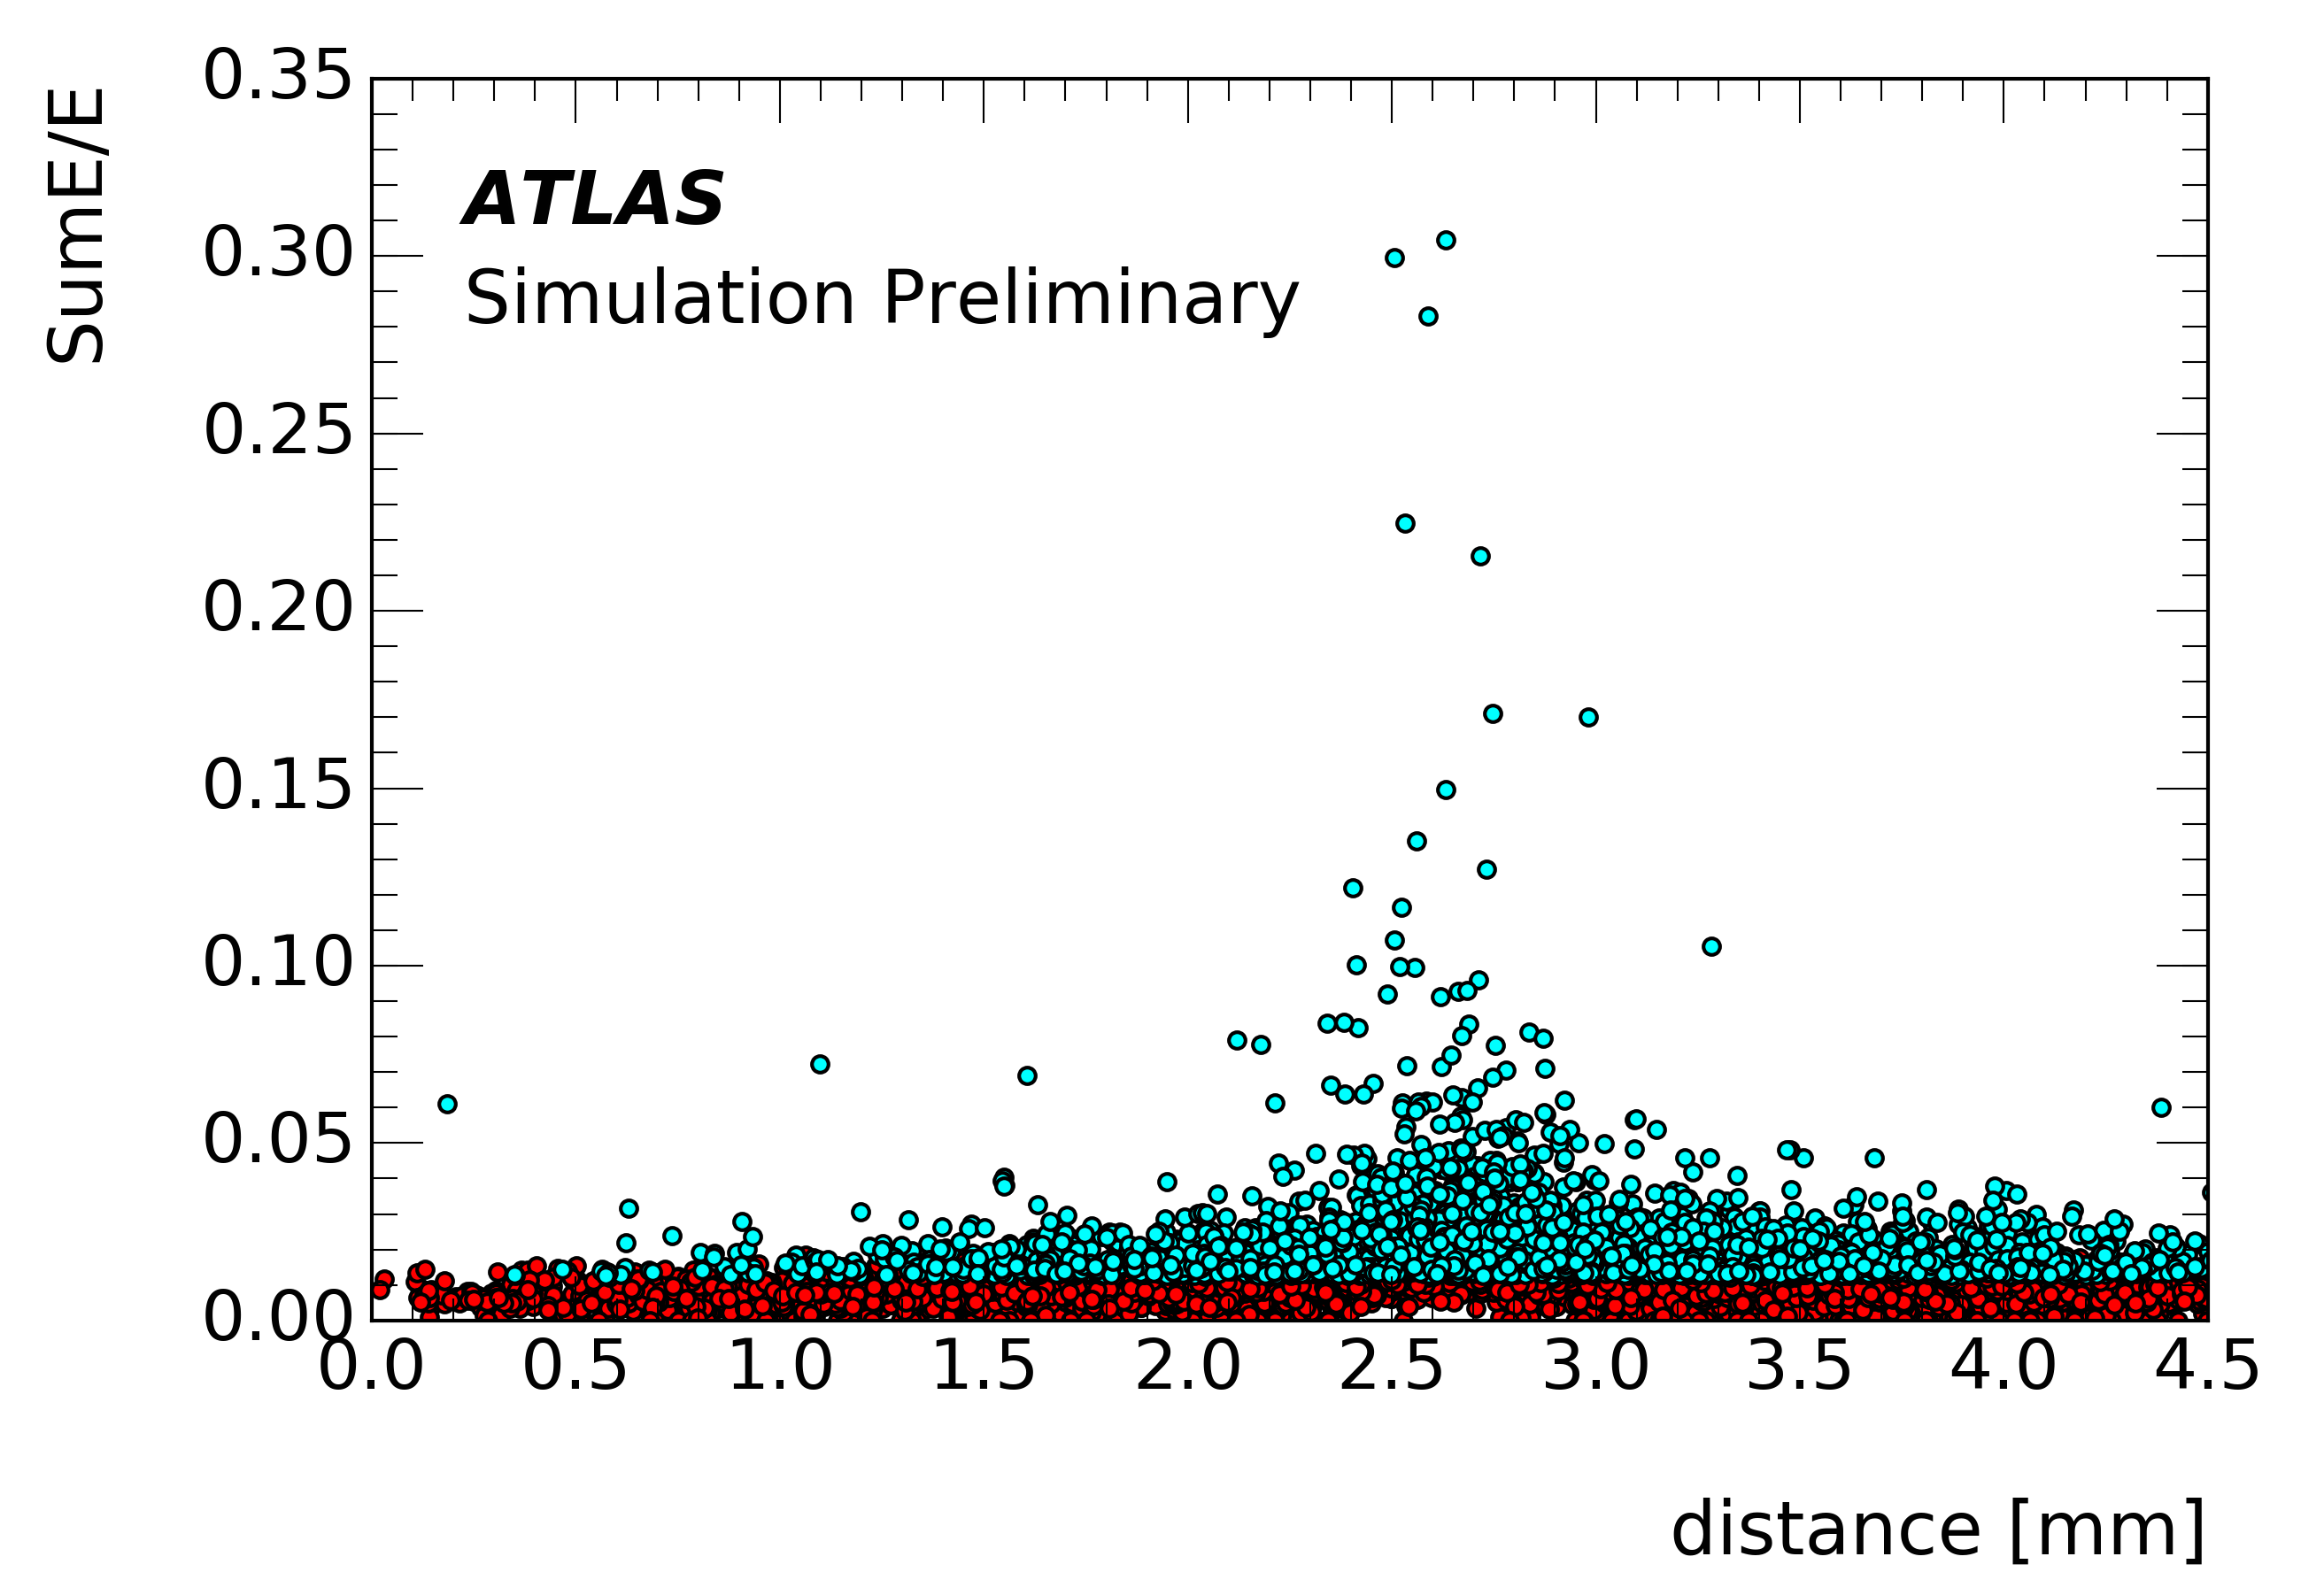
\includegraphics[width=1.\linewidth]{MC/firstClassifier.png} \\ a)}
\end{minipage}
\hfill
\begin{minipage}[h]{0.49\linewidth}
\center{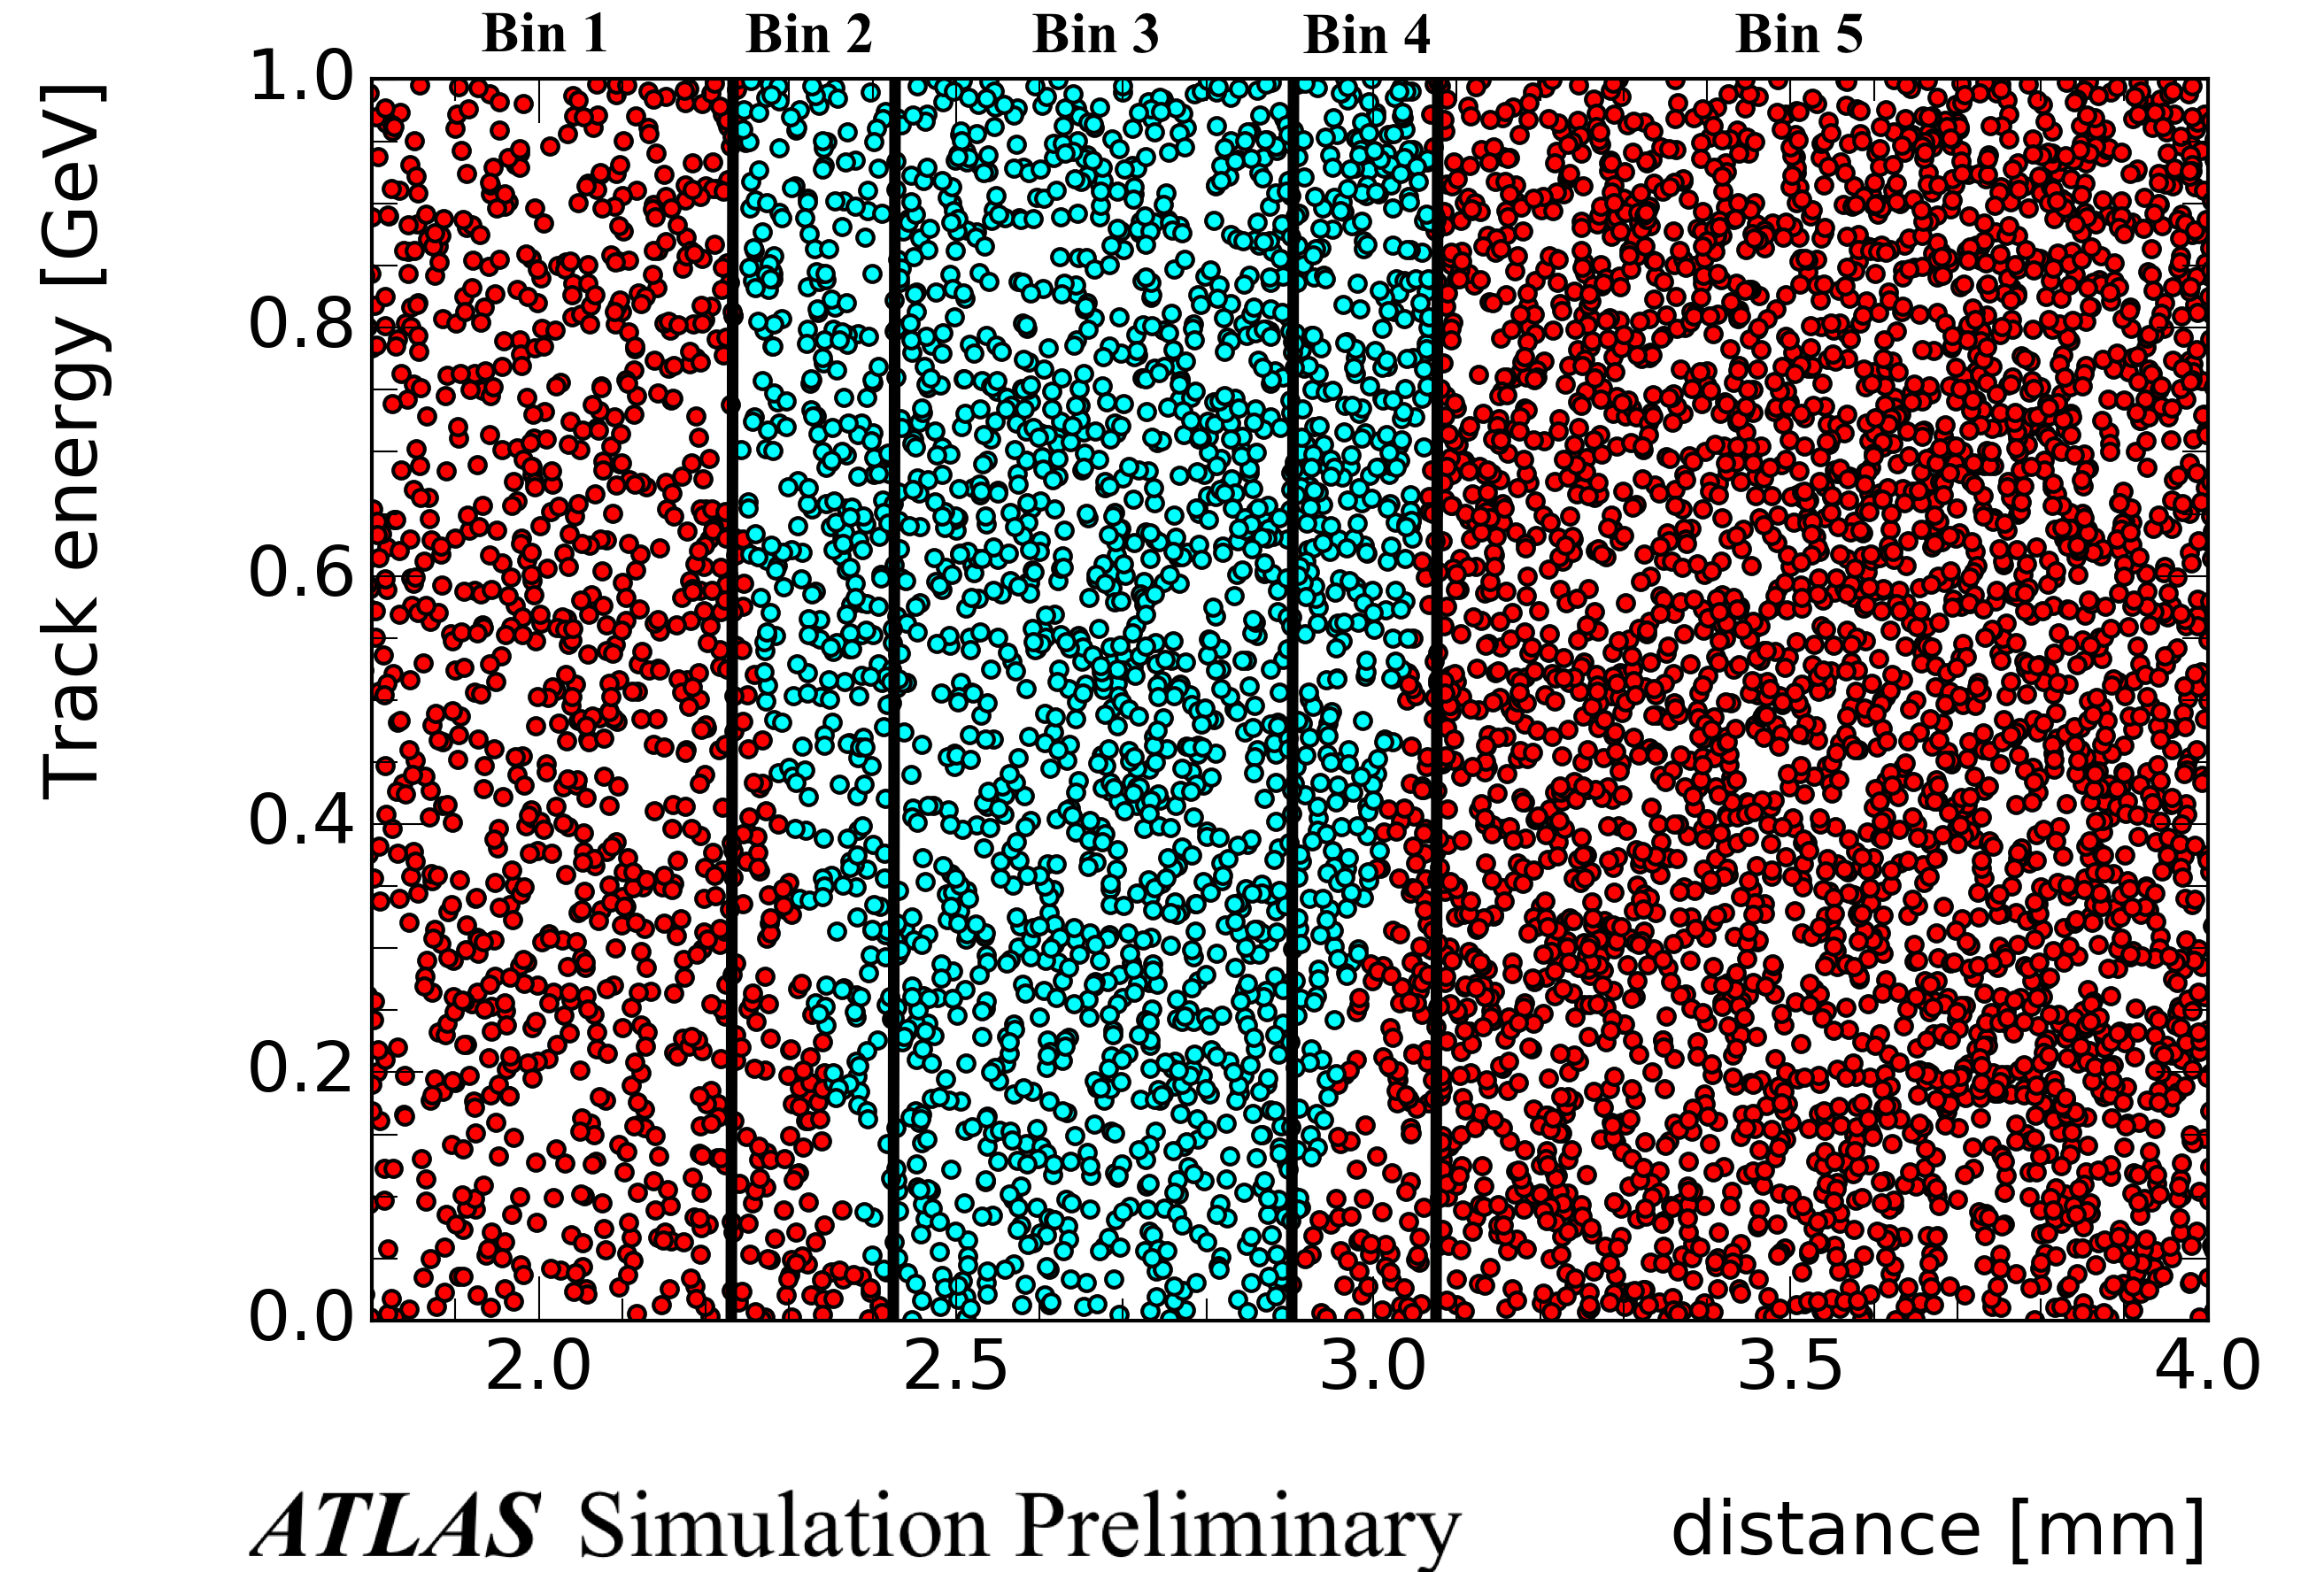
\includegraphics[width=1.\linewidth]{MC/secondClassifier.png} \\ b)}
\end{minipage}
\caption{Results of machine learning algorithm classification for a) first classifier b) second classifier. Cyan dots correspond to sensitive material showers, red to dead material showers. The black lines in Fig. b correspond to the resulting bin positions.}
\label{fig:Class}
\end{figure}

The second classifier uses predictions of the first classifier as input label. 

It reconstructs a best dividing hyperplane between two types of shower using a support vector machines. It uses as input the truth parameters of the electron, e.g. energy of the initial electron and its distance to the closest rod center. Different kernels have been tested and the best predictions have been obtained using RBF kernel (Eq. \ref{eq:RBF}).  Assuming, that $\eta^{momentum} \approx \eta^{position}$ a classification is performed in each $\eta^{distance}$ bin used in the library. 

An example of the classifier output is shown in a Fig. \ref{fig:Class} b). The obtained gap positions are wider, than the original ones, as it is expected from the model.  Variation of the obtained parameters have been found small, so the mean of the parameters has been as an input for the binning.  

\subsection{Interpretation of results}

Since full new regeneration of libraries and the validation of reconstructed variables is time-consuming procedure, a Monte Carlo method has been developed for a cross-check of the classifiers and its interpretation. It uses pseudorapidity $\eta^{position}$, energy of electron and distance to the closest rod center from the data as a reference for the random generator. This simulation allows to compare the shower energies and shower energies divided by  the energy of the initial electron (SumE/E) distributions with the distributions coming from the full simulation, which are considered as a reference.

The resulting hyperplane from second classifier can be translated to the bin positions in the different ways. Several interpretations of the bin positions have been tested and the best one is shown in Fig.~\ref{fig:Class} b) with black lines. The best SumE/E agreemen have been achieved using three bins in liquid argon position instead of the only one. The central bin, according to the classifier, contains just sensitive material showers events, while the other two there is a mixture of dead and sensitive material showers. The obtained positions of the liquid argon bins are wider, than the nominal ones for both FCAL1 and FCAL2.

Comparison of SumE/E distributions using toy MC on old libraries (Fig. ~\ref{fig:Interpret} a) and the libraries with the new binning (Fig. ~\ref{fig:Interpret} b) has shown, that we could expect a better performance on the reconstructed values for the new binning.

\begin{figure}[!tbp]
\begin{minipage}[h]{0.49\linewidth}
\center{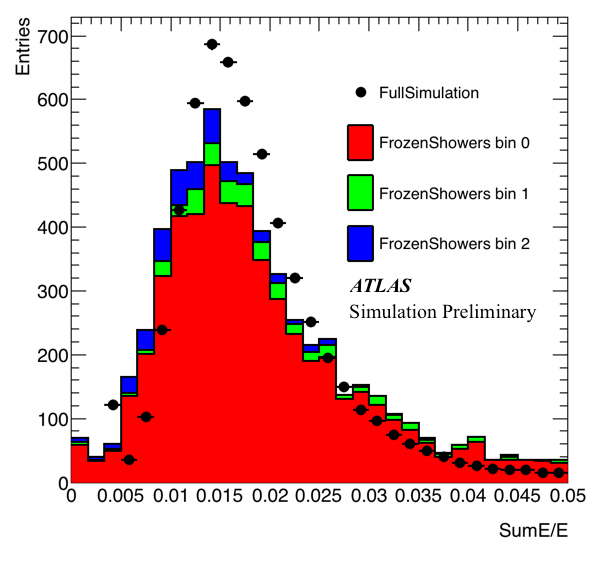
\includegraphics[width=1.\linewidth]{MC/oldSumE.png} \\ a)}
\end{minipage}
\hfill
\begin{minipage}[h]{0.49\linewidth}
\center{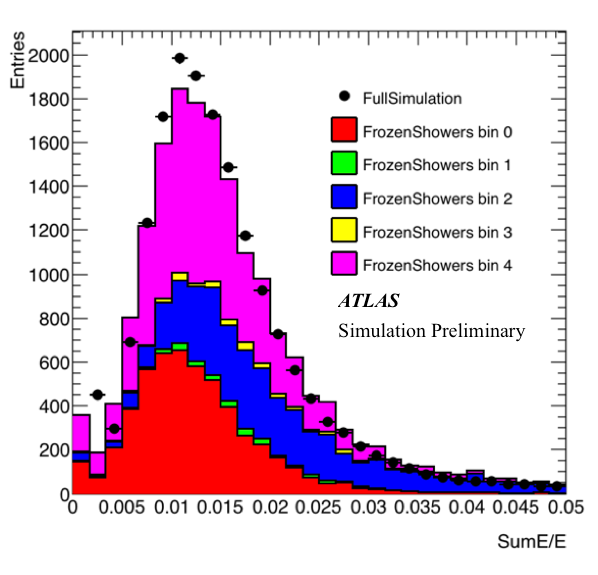
\includegraphics[width=1.\linewidth]{MC/newSumE.png} \\ b)}
\end{minipage}
\caption{Comparison of the distributions of shower energy divided by  the energy of the initial electron between full simulation and toy MC using libraries for liquid argon gap bins and 2 closest to them bins for a) old "tuned" libraries with 1 liquid argon gap bin  b) new libraries using 3 liquid argon gap bins. There are still remaining differences between full simulation and toy MC, but the new machine learning binning gives a better agreement with full simulation.}
\label{fig:Interpret}
\end{figure}


\subsection{Reconstructed electron energy}

Since the resolution of the single electrons can have a significant difference, the energies of reconstructed electrons are validated before the mass validation of the different groups. Measurement of the shift in the mean energy between full and fast simulation allows to correct the scale for frozen showers.

Validation is performed for the following electron energies: 100 GeV, 200 GeV, 500 GeV and 1000 GeV and within the $\eta$ directions that are corresponding to the 12 $\eta$ bins of the library. The resolution is calculated as RMS of all reconstructed energies for the certain energy and $\eta$. The results of the electron resolution validation for the new machine learning based binning and old "tuned" libraries is shown in Fig. \ref{fig:Reso}. The new methods gives a better of comparable resolution agreement than an old libraries. However, there are 2 bins, there new method resolution is significantly worse, than old one (3.5 and 4.3). This means, that this method still needs to be improved. The possible ways of its improvement are discussed in Sec. \ref{sec:FSImpr}.

In a meanwhile it was decided to use a combination of the new and old libraries. The mean shift is corrected as described in Sec. \ref{sec:LibTuning} and showed in Fig. \ref{fig:Mean}. The remaining differences between full and fast simulation are considered negligible.


\begin{figure}[!tbp]
\begin{minipage}[h]{0.32\linewidth}
\center{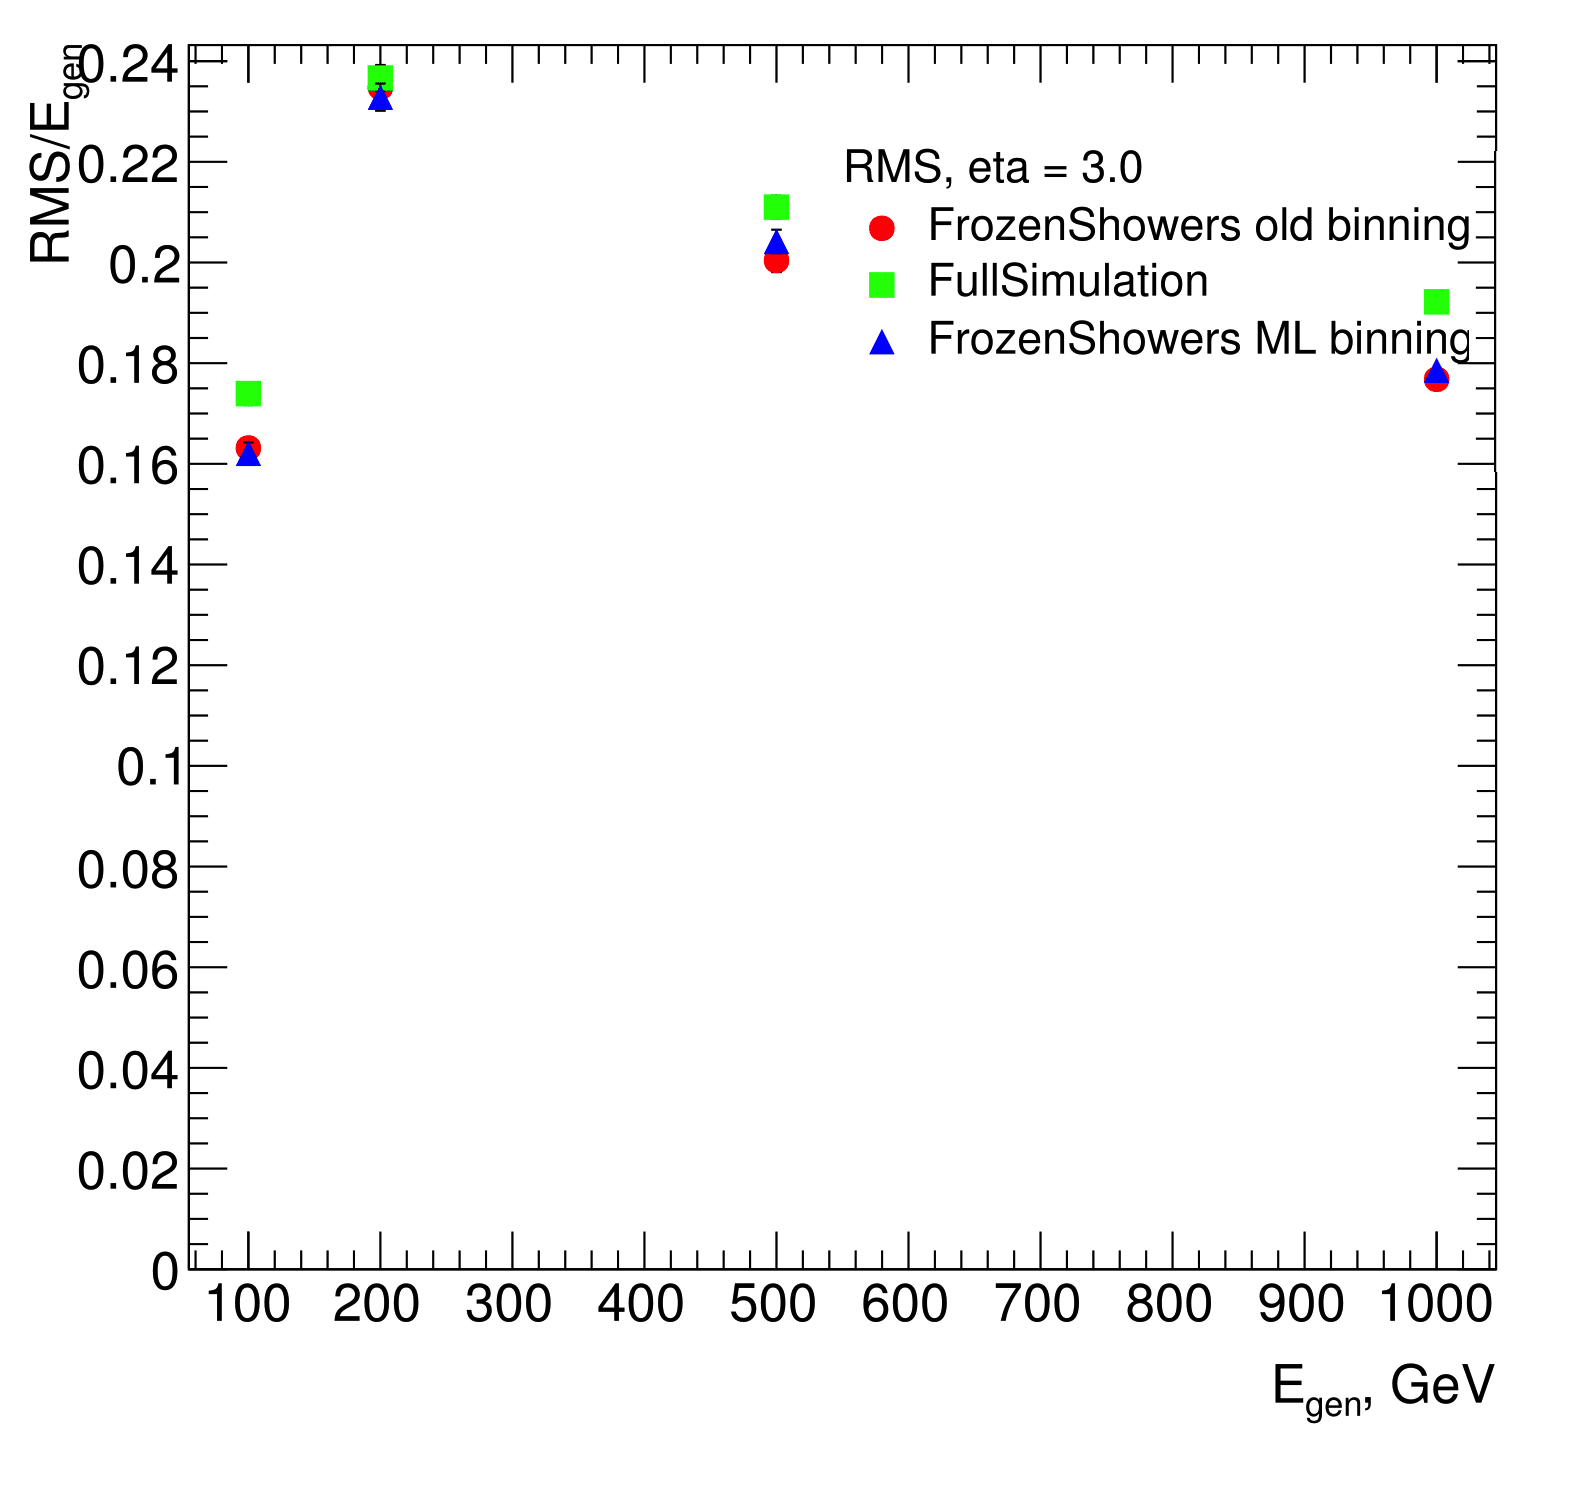
\includegraphics[width=1.\linewidth]{MC/RMS/RMS-12.png} }
\end{minipage}
\hfill
\begin{minipage}[h]{0.32\linewidth}
\center{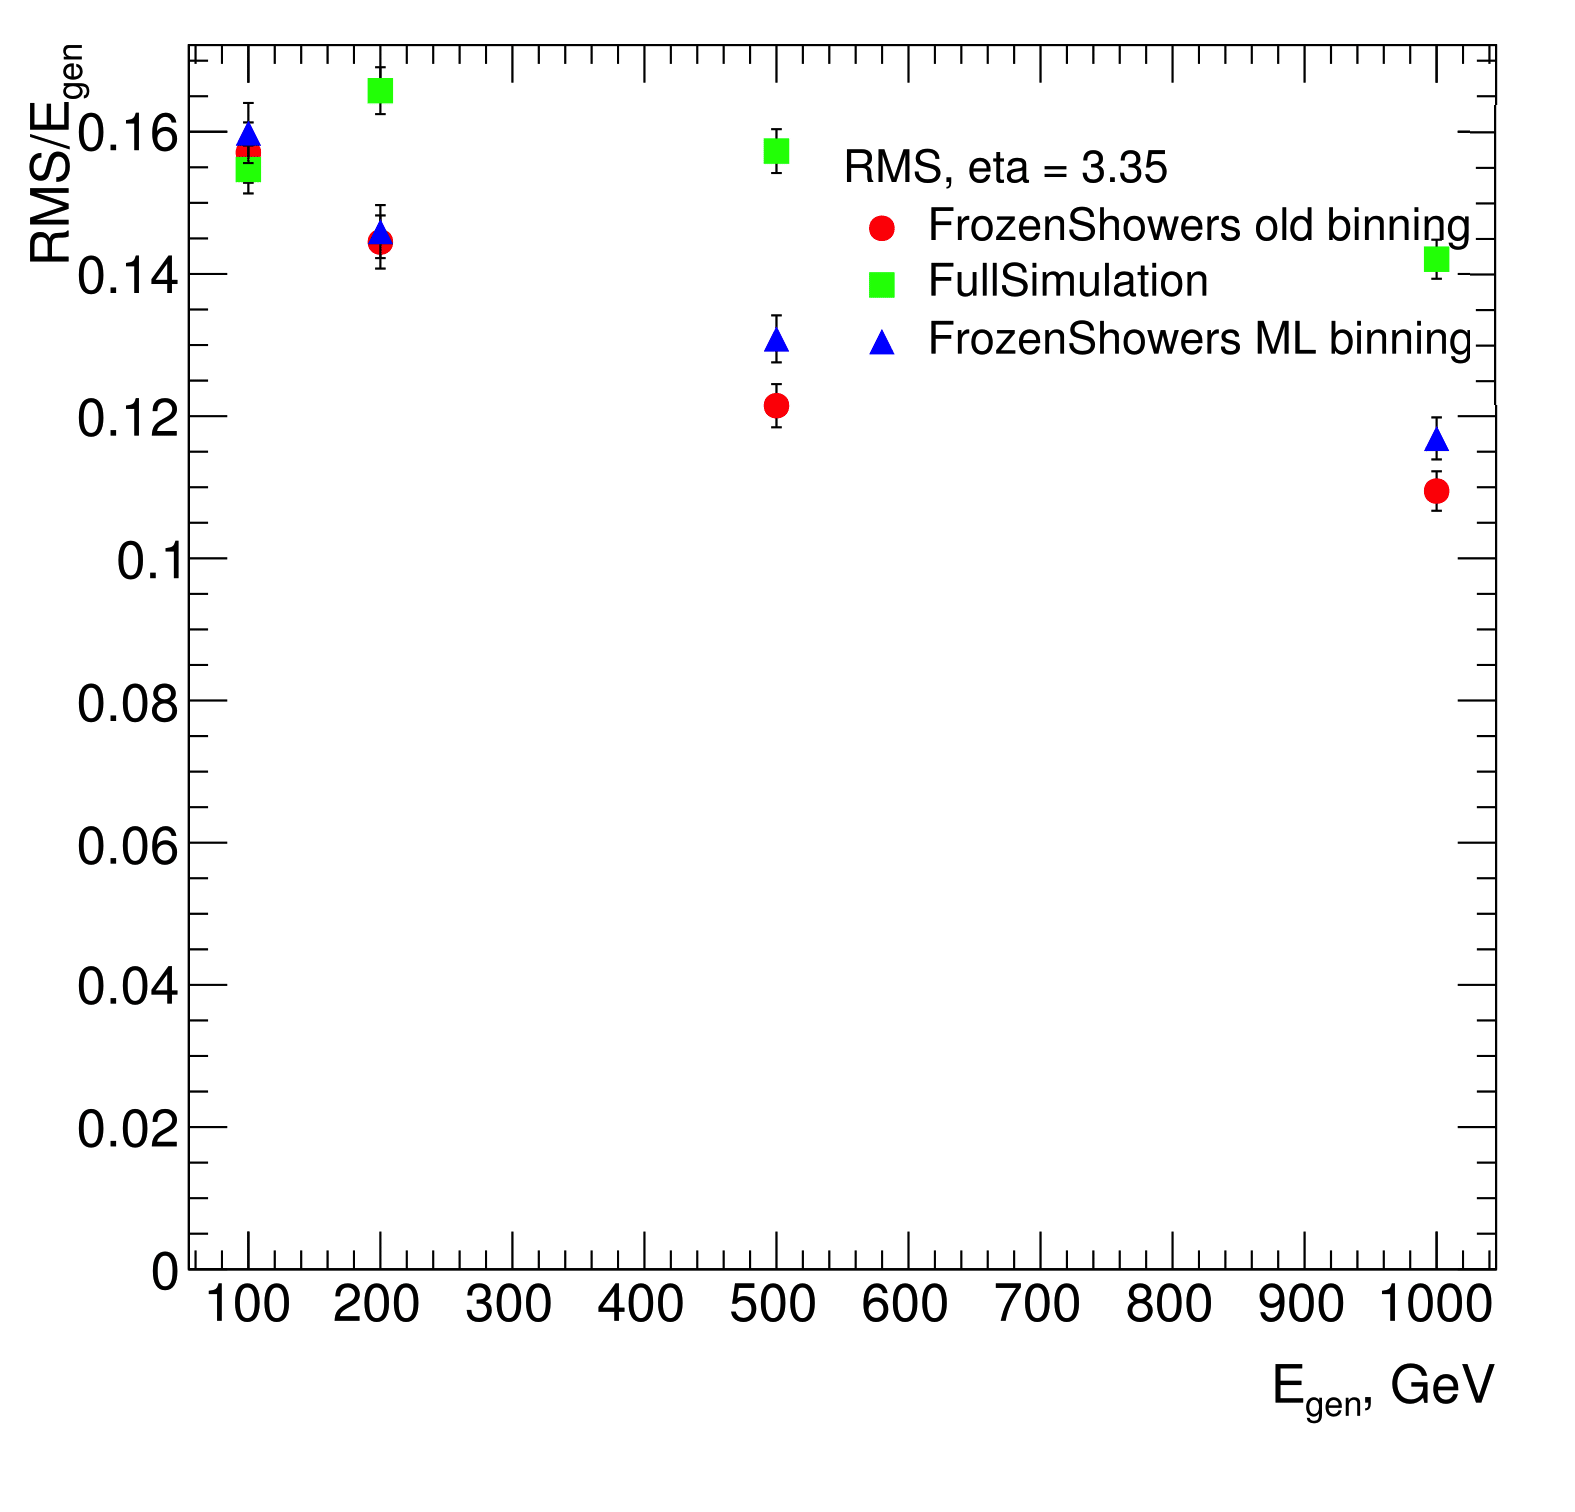
\includegraphics[width=1.\linewidth]{MC/RMS/RMS-11.png} }
\end{minipage}
\hfill
\begin{minipage}[h]{0.32\linewidth}
\center{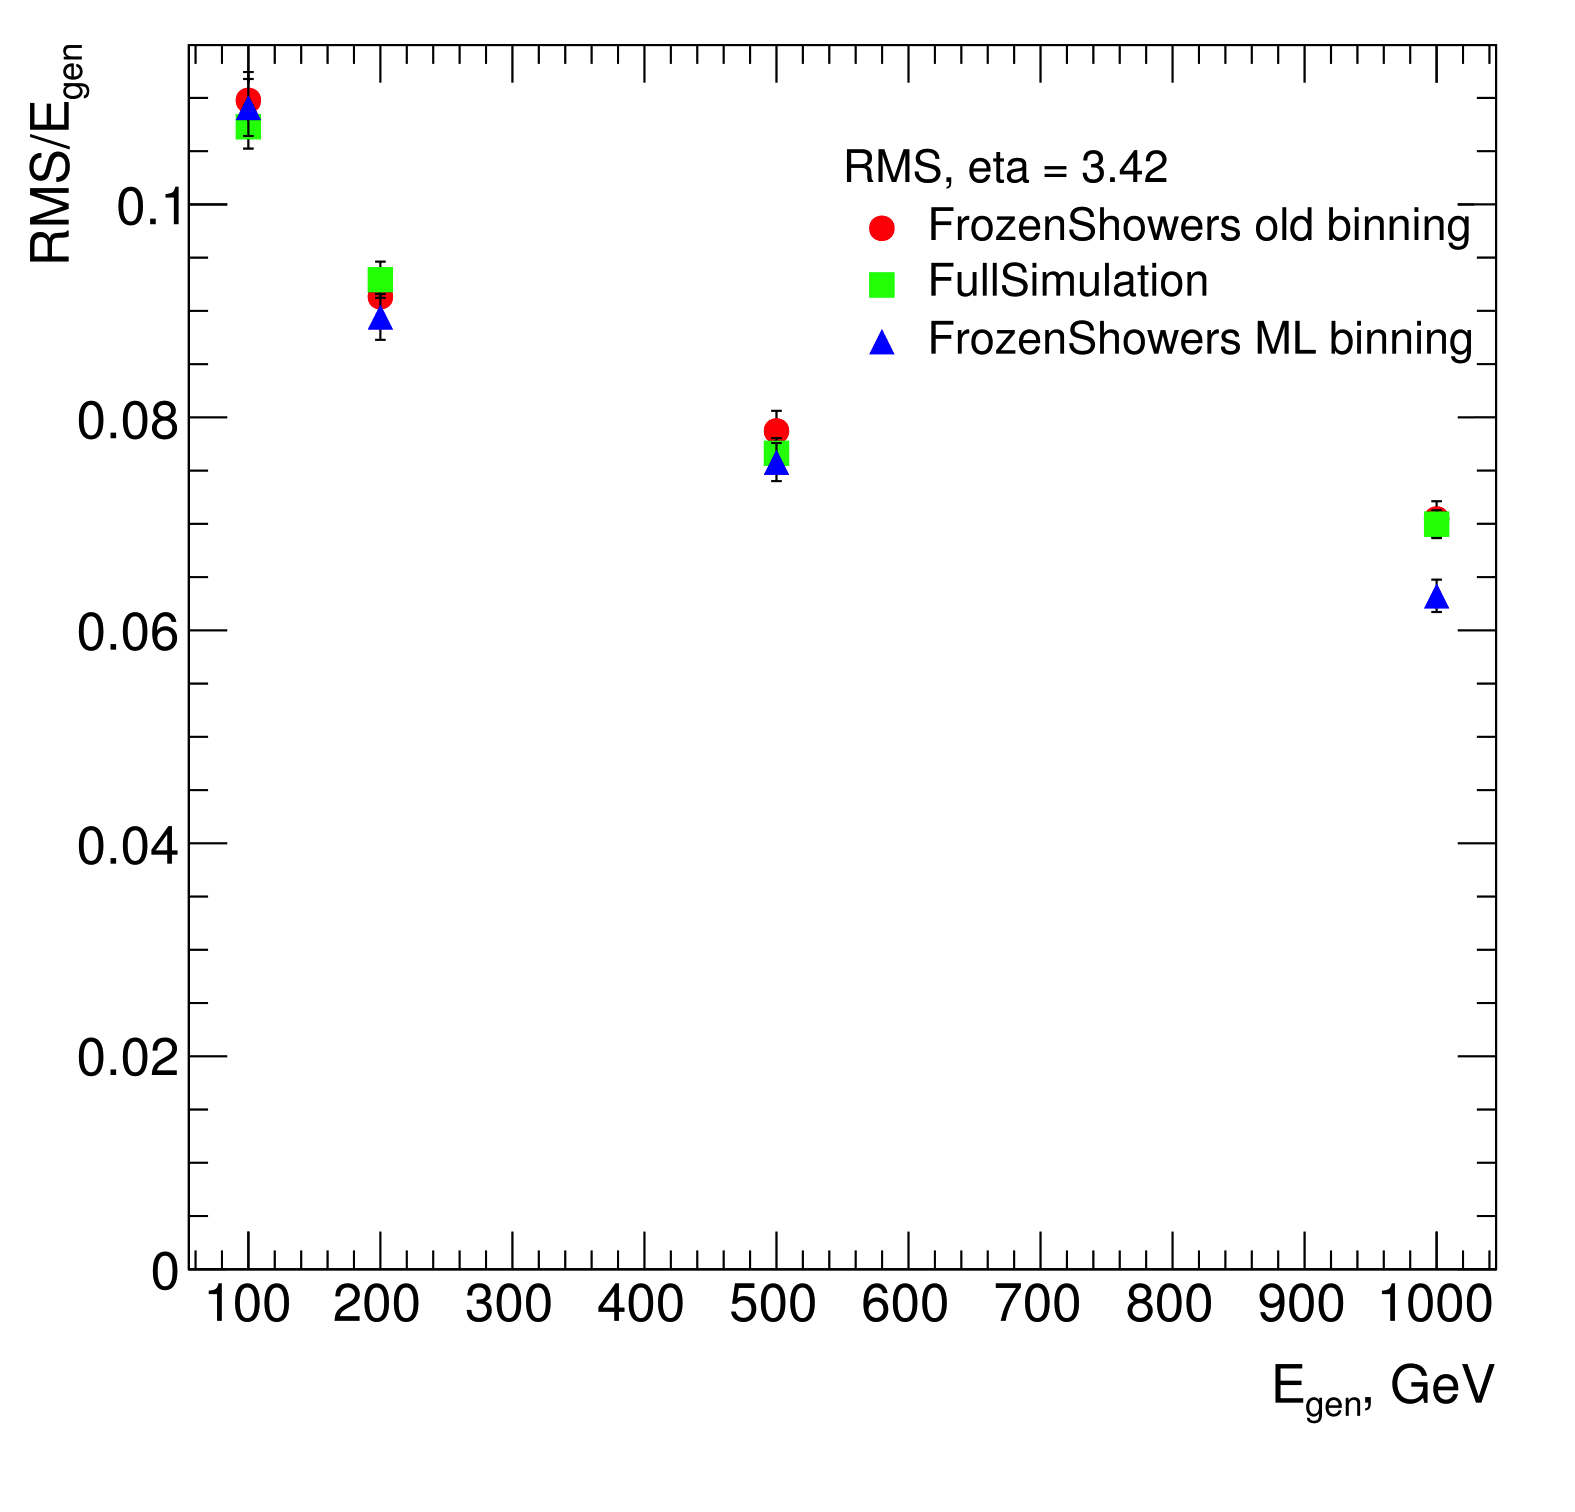
\includegraphics[width=1.\linewidth]{MC/RMS/RMS-10.png}  }
\end{minipage}
\vfill
\begin{minipage}[h]{0.32\linewidth}
\center{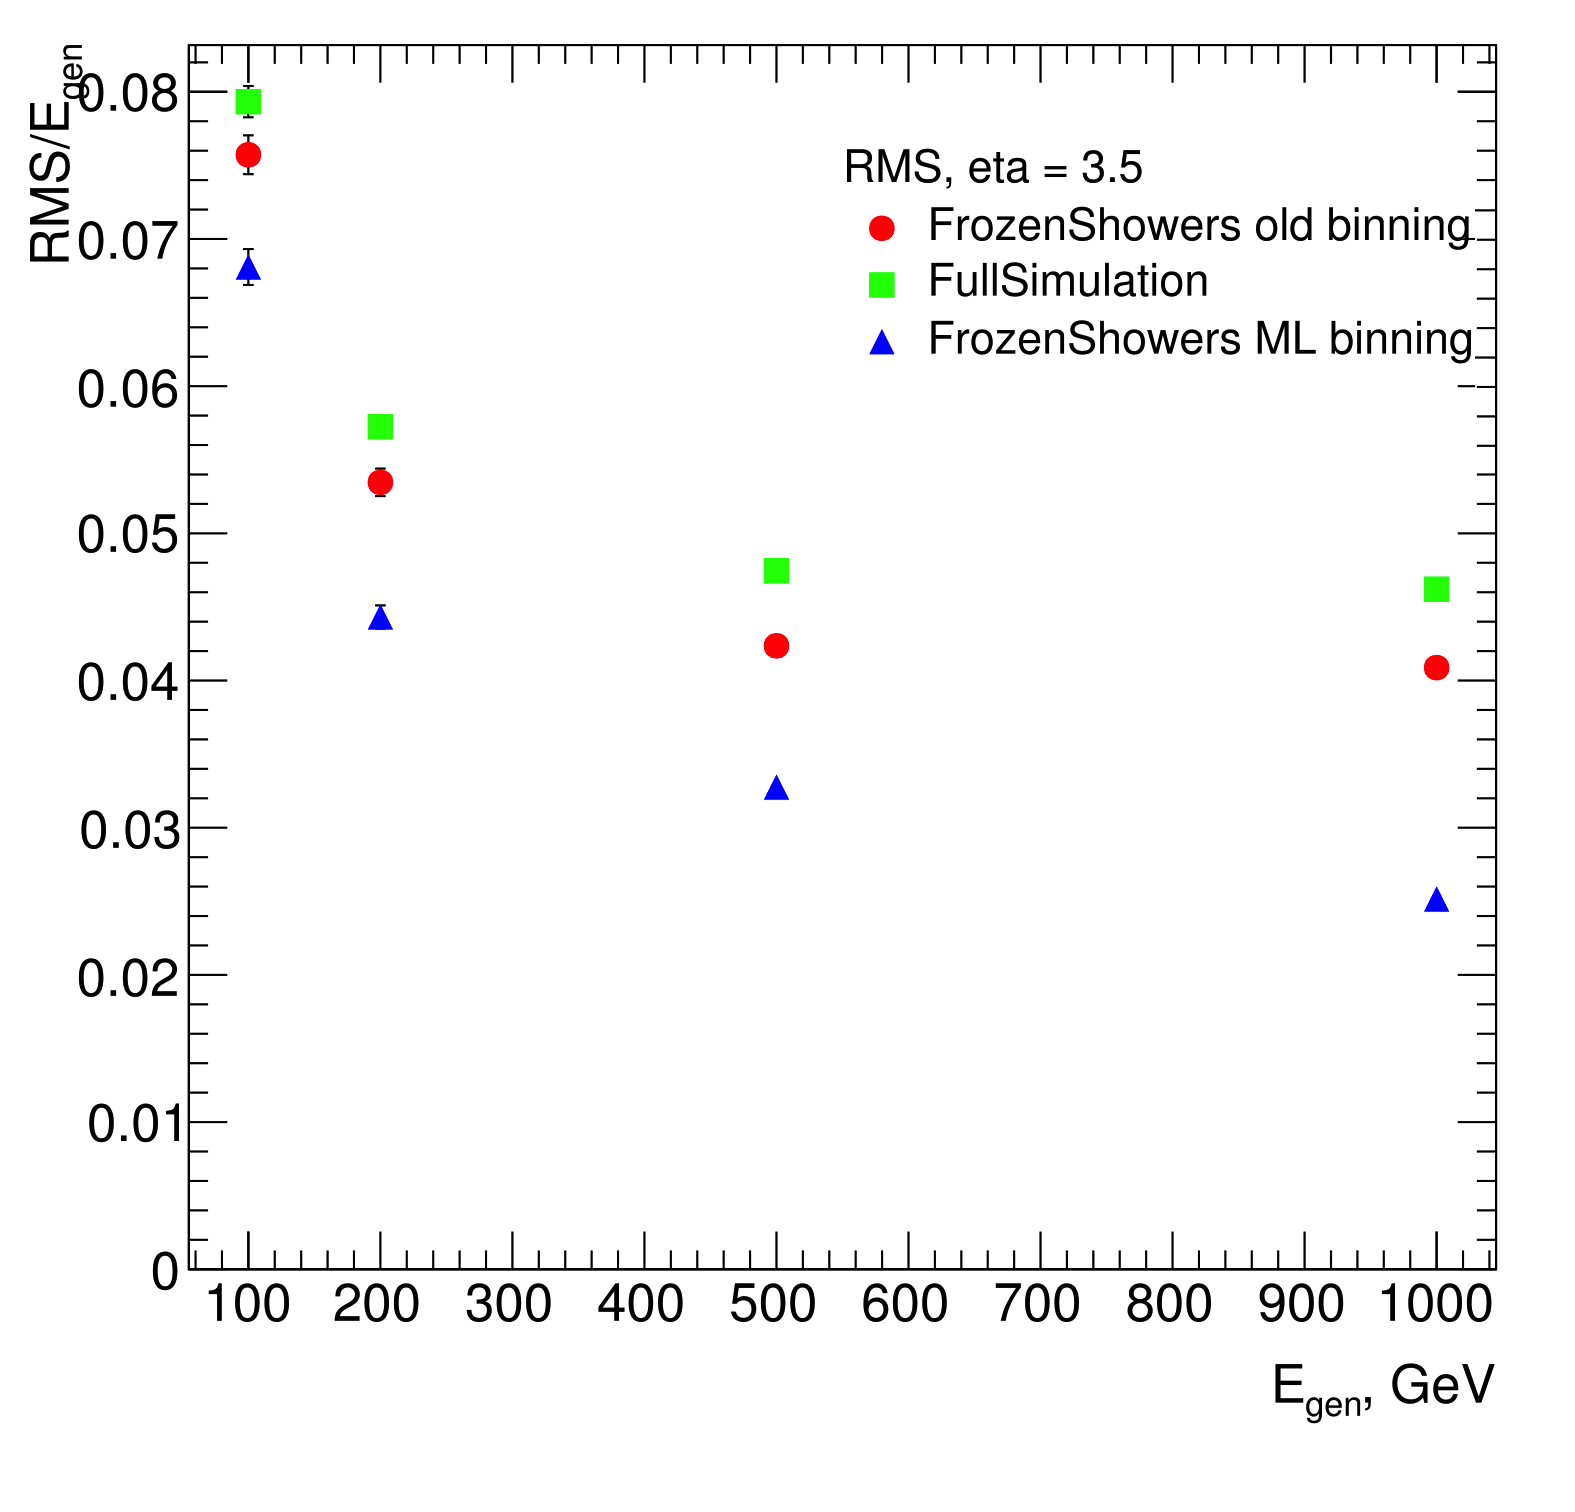
\includegraphics[width=1.\linewidth]{MC/RMS/RMS-09.png}  }
\end{minipage}
\hfill
\begin{minipage}[h]{0.32\linewidth}
\center{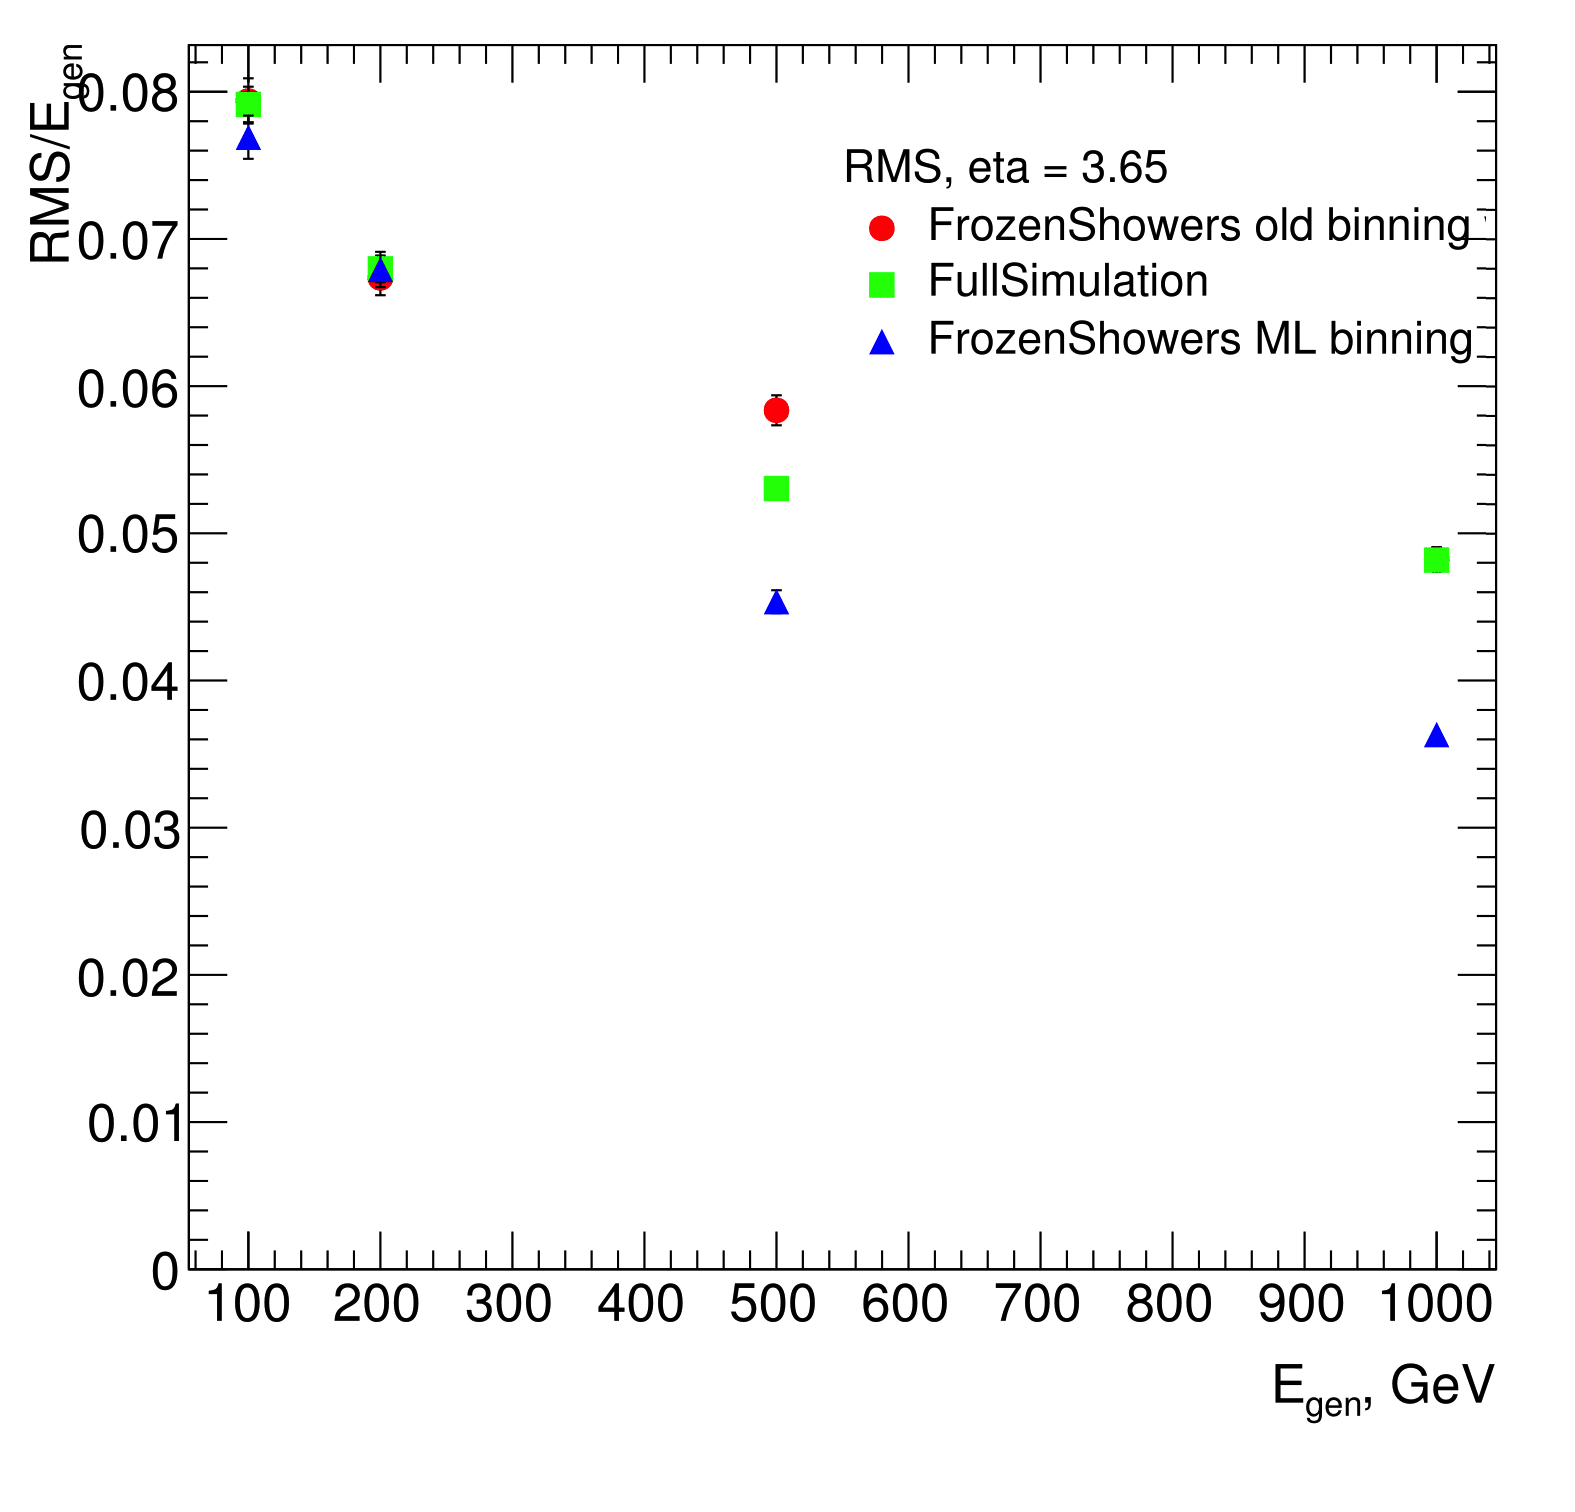
\includegraphics[width=1.\linewidth]{MC/RMS/RMS-08.png} }
\end{minipage}
\hfill
\begin{minipage}[h]{0.32\linewidth}
\center{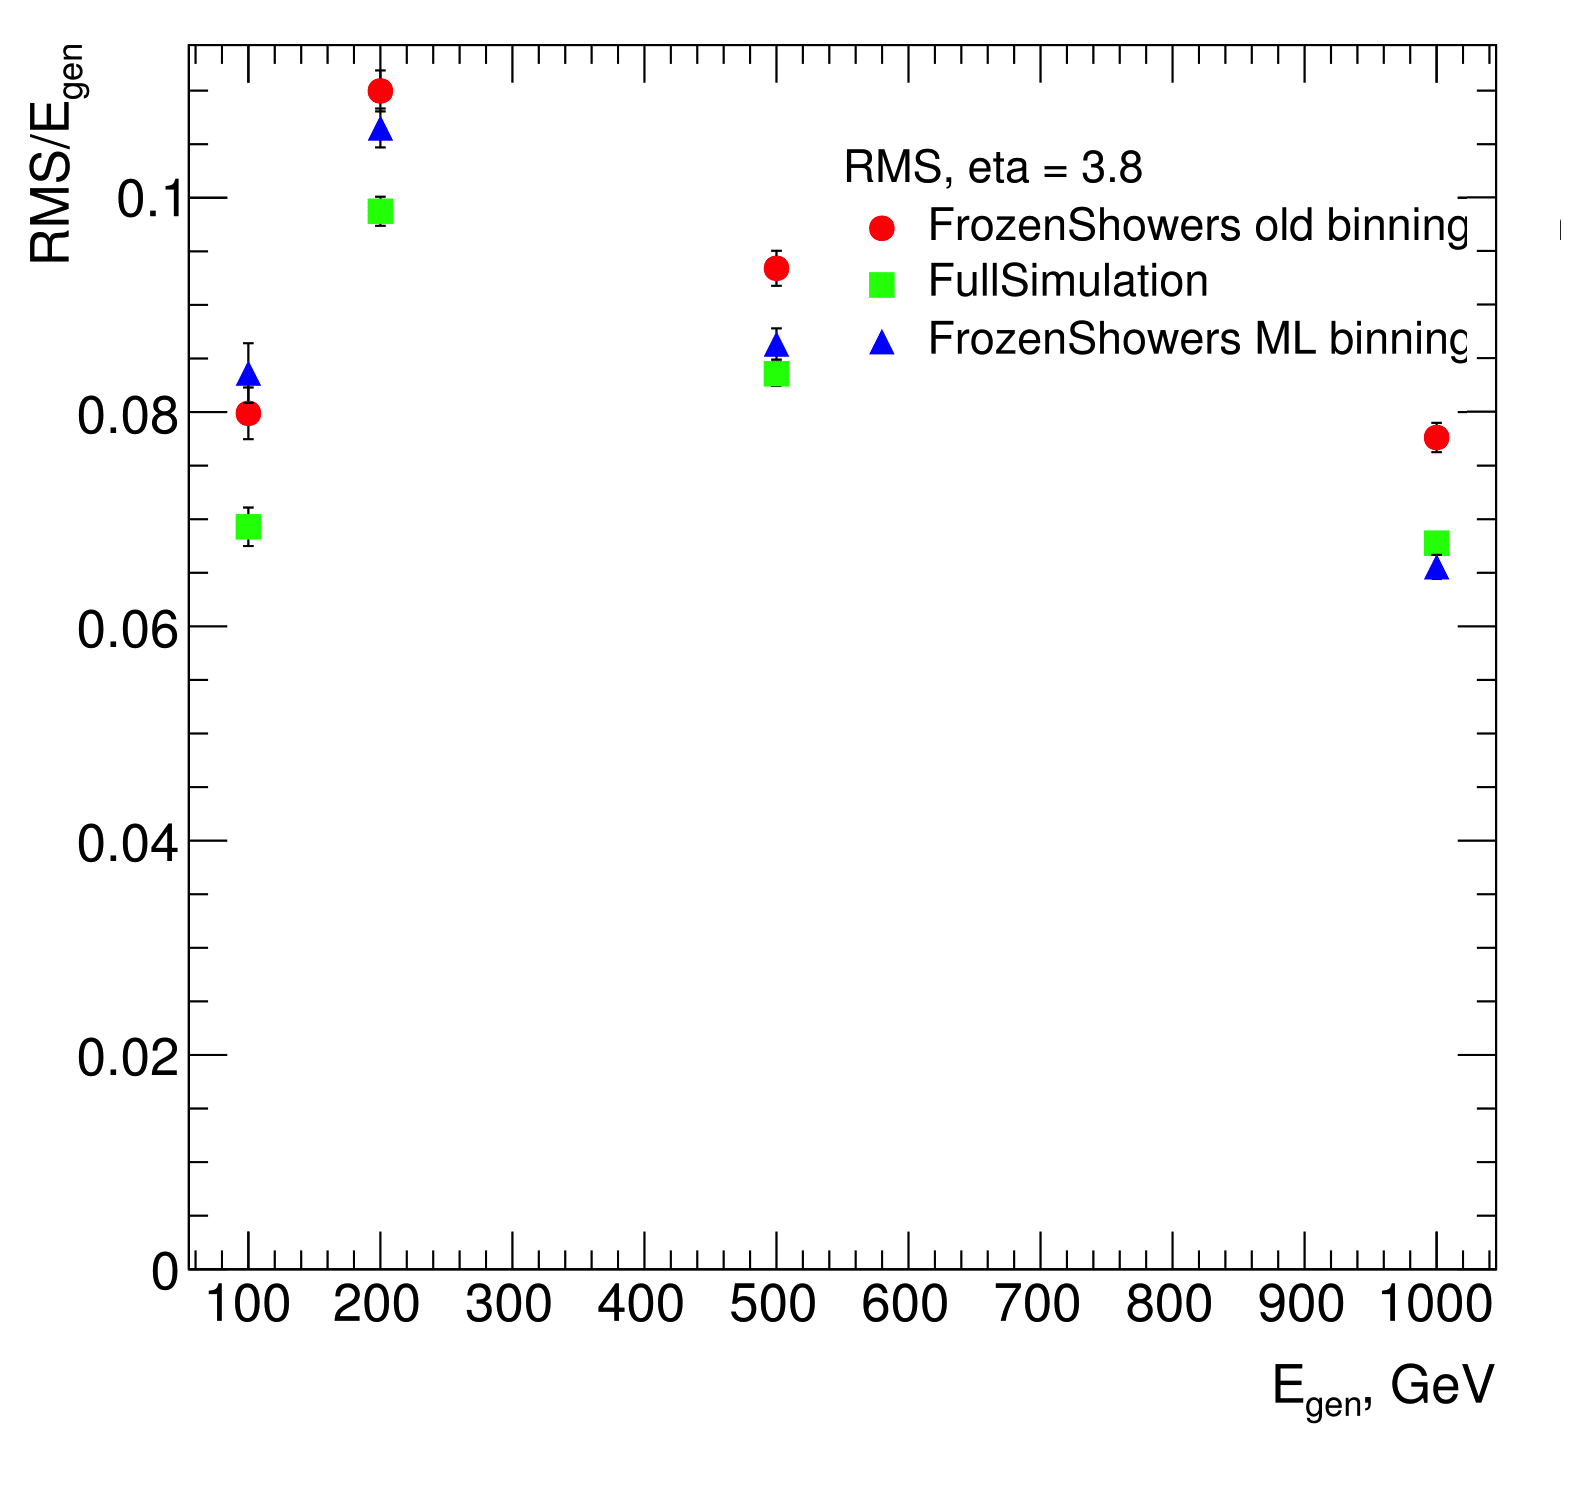
\includegraphics[width=1.\linewidth]{MC/RMS/RMS-07.png}  }
\end{minipage}
\vfill
\begin{minipage}[h]{0.32\linewidth}
\center{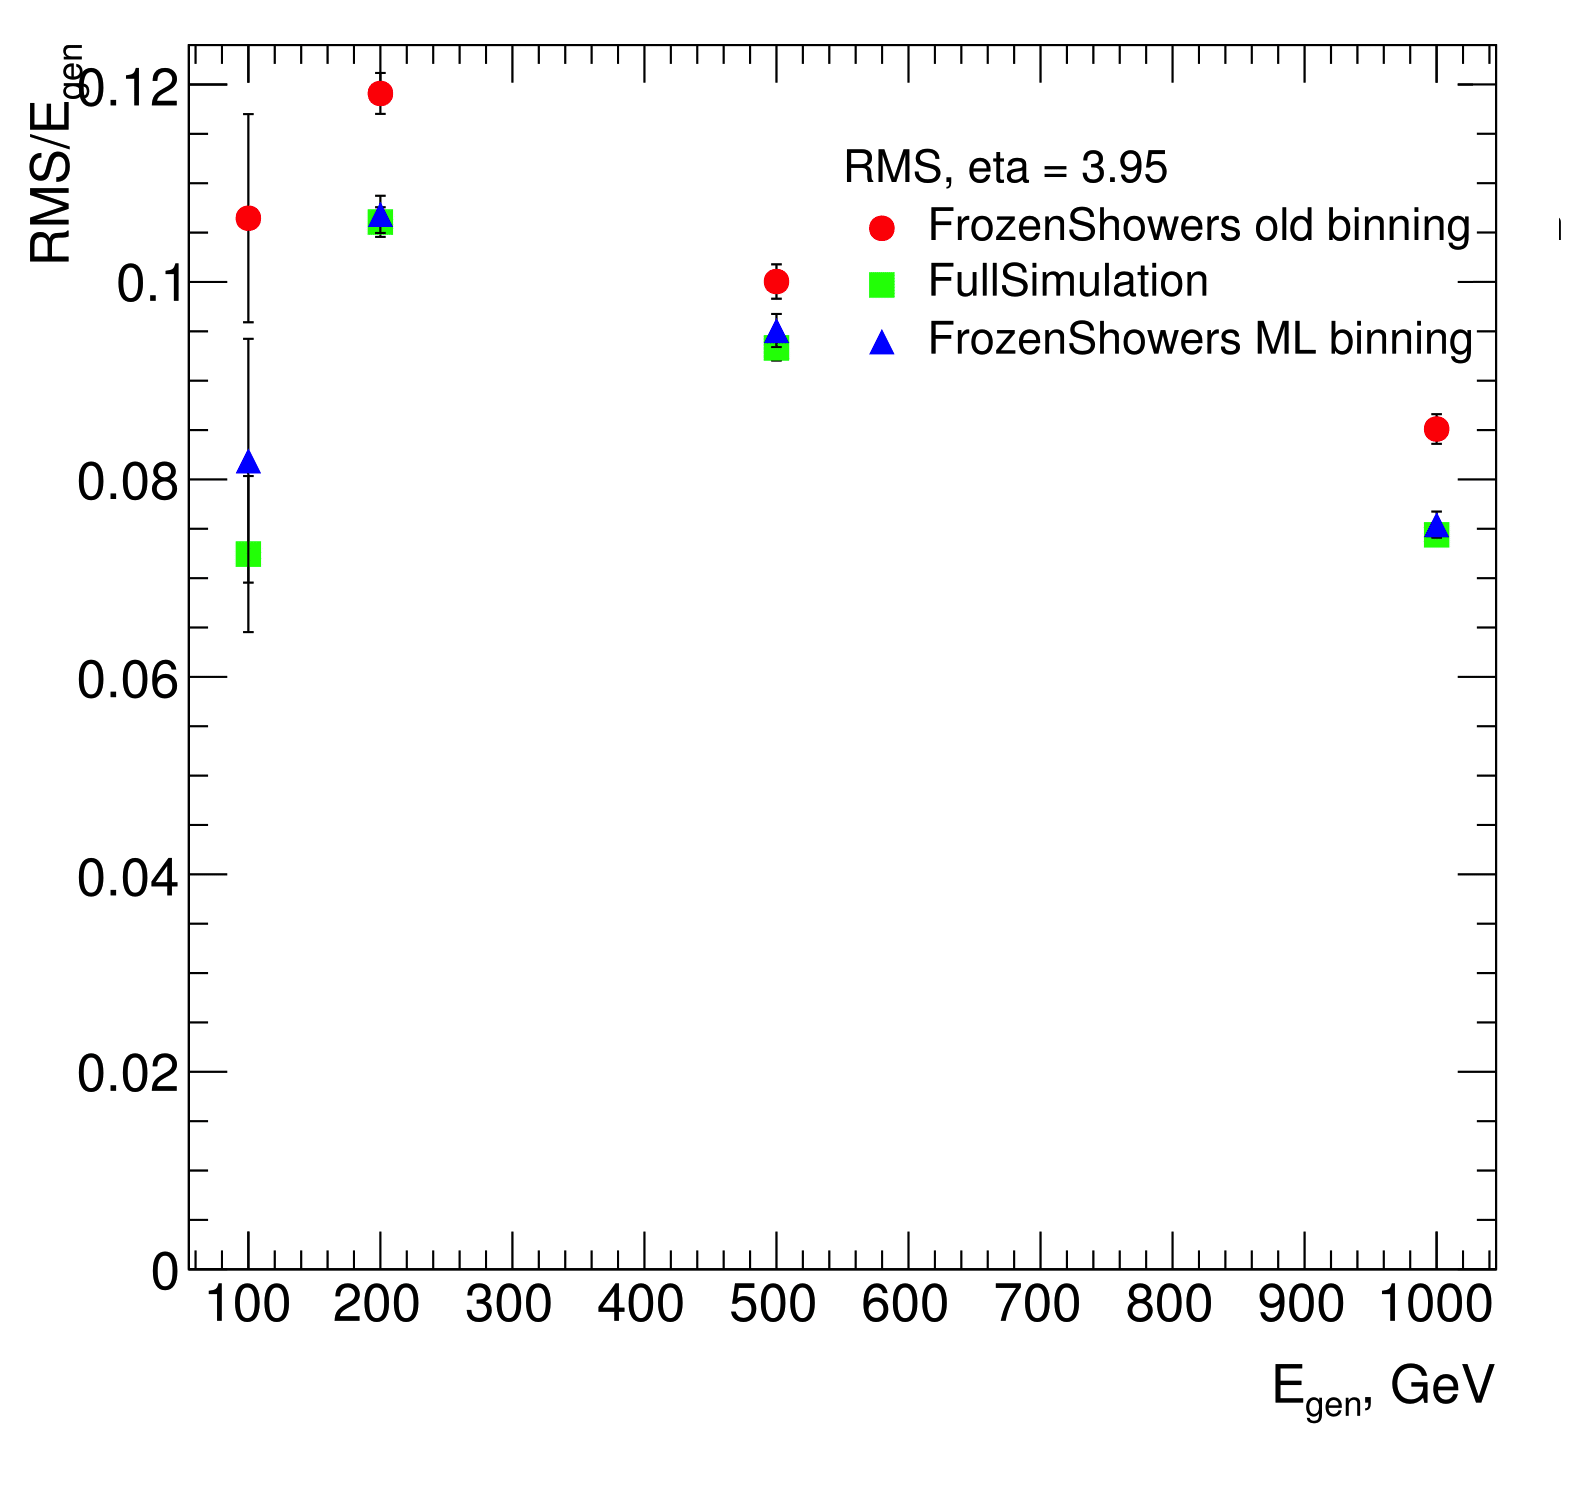
\includegraphics[width=1.\linewidth]{MC/RMS/RMS-06.png}  }
\end{minipage}
\hfill
\begin{minipage}[h]{0.32\linewidth}
\center{\includegraphics[width=1.\linewidth]{MC/RMS/RMS-05.png}  }
\end{minipage}
\hfill
\begin{minipage}[h]{0.32\linewidth}
\center{\includegraphics[width=1.\linewidth]{MC/RMS/RMS-04.png}  }
\end{minipage}
\vfill
\begin{minipage}[h]{0.32\linewidth}
\center{\includegraphics[width=1.\linewidth]{MC/RMS/RMS-03.png}  }
\end{minipage}
\hfill
\begin{minipage}[h]{0.32\linewidth}
\center{\includegraphics[width=1.\linewidth]{MC/RMS/RMS-02.png} }
\end{minipage}
\hfill
\begin{minipage}[h]{0.32\linewidth}
\center{\includegraphics[width=1.\linewidth]{MC/RMS/RMS-01.png} }
\end{minipage}
\caption{Energy resolution of reconstructed electrons for full simulation, new libraries with ML binning and old tuned libraries with original binning for different $\eta$ bins }
\label{fig:Reso}
\end{figure}

\begin{figure}[!tbp]
\begin{minipage}[h]{0.32\linewidth}
\center{\includegraphics[width=1.\linewidth]{MC/Mean/Mean-12.png} }
\end{minipage}
\hfill
\begin{minipage}[h]{0.32\linewidth}
\center{\includegraphics[width=1.\linewidth]{MC/Mean/Mean-11.png}  }
\end{minipage}
\hfill
\begin{minipage}[h]{0.32\linewidth}
\center{\includegraphics[width=1.\linewidth]{MC/Mean/Mean-10.png}  }
\end{minipage}
\vfill
\begin{minipage}[h]{0.32\linewidth}
\center{\includegraphics[width=1.\linewidth]{MC/Mean/Mean-09.png}  }
\end{minipage}
\hfill
\begin{minipage}[h]{0.32\linewidth}
\center{\includegraphics[width=1.\linewidth]{MC/Mean/Mean-08.png}  }
\end{minipage}
\hfill
\begin{minipage}[h]{0.32\linewidth}
\center{\includegraphics[width=1.\linewidth]{MC/Mean/Mean-07.png}  }
\end{minipage}
\vfill
\begin{minipage}[h]{0.32\linewidth}
\center{\includegraphics[width=1.\linewidth]{MC/Mean/Mean-06.png}  }
\end{minipage}
\hfill
\begin{minipage}[h]{0.32\linewidth}
\center{\includegraphics[width=1.\linewidth]{MC/Mean/Mean-05.png}  }
\end{minipage}
\hfill
\begin{minipage}[h]{0.32\linewidth}
\center{\includegraphics[width=1.\linewidth]{MC/Mean/Mean-04.png}  }
\end{minipage}
\vfill
\begin{minipage}[h]{0.32\linewidth}
\center{\includegraphics[width=1.\linewidth]{MC/Mean/Mean-03.png}  }
\end{minipage}
\hfill
\begin{minipage}[h]{0.32\linewidth}
\center{\includegraphics[width=1.\linewidth]{MC/Mean/Mean-02.png}  }
\end{minipage}
\hfill
\begin{minipage}[h]{0.32\linewidth}
\center{\includegraphics[width=1.\linewidth]{MC/Mean/Mean-01.png}  }
\end{minipage}
\caption{Shift of the reconstructed energy to the truth energy of electrons for full simulation, new FS libraries with ML binning and full simulation for different $\eta$ bins }
\label{fig:Mean}
\end{figure}

\subsection{Plans for the future}\label{sec:FSImpr}

The validation have showed a good agrement between full simulation and fast simulation for most of the bins, however, because not all of the bins are performing equally well, the additional modifications of the algorithm are needed. The following modifications have been investigated and planned to be performed in the nearest future:
\begin{itemize}
\item Procedure with $\eta$ dependent bin size. Currently all of the bins have the same size and position of the liquid argon bin. However, because of the outlying bins, the procedure should be modified and determine the bin position separately for each bin.
\item Use of the closer to real case for training sample. The problem of electron resolution could be also caused by too simlified models, used to train on. It is planned to repeat the procedure for training sample with distributions, closer to the nominal ones.
\item Adding the direction of the shower binned variable. Since there is a complicated dependency between position of the electron and its direction (especially in small energy region), the additional binning could solve the remaining problems with electron energy resolution.
\end{itemize}

\section{Validation of the new libraries}\label{sec:FSValidation}

The good fast simulation method should work equally good on all types of reconstructed objects, this is why for each new frozen showers libraries production an new iteration of mass validation is performed. The validation is done separately for each object by the different groups by comparing the distibutions obtained from full and fast simulation

Frozen showers have been validated on following objects and showed a good agreement:
\begin{itemize}
\item Z bosons from $Z \to ee$ sample with one central and one forward electrons(Fig. \ref{fig:OtherVal} a). The resolution of Z-mass peak is dominated by the resolution of the central electron, so Z boson is mostly sensitive just to the mean energy of the forward electrons. There is visible shift in the mass distribution between data and Monte-Carlo, that however, is within tolerable region.
\item Jets form two jet events. The validation have showed a good agreement for all of the variables. The distribution of the jet response (Fig. \ref{fig:OtherVal} b) showed, that Frozen Showers method does not change the jet scale.
\item Topo clusters from $t\bar{t}$ events. 
\item Forward electrons. The forward electrons validation have showed, that usage of the frozen showers is not changing the $\eta$ and $E_{T}$ distributions of the forward electrons. Studies of forward electrons resolution have been performed separately and will be discussed in the previous section.
\end{itemize}
The total agreement between full and fast simulation for different objects makes a Frozen Showers method applicable for a MC production in 2016.

\begin{figure}[!tbp]
\begin{minipage}[h]{0.49\linewidth}
\center{\includegraphics[width=1.\linewidth]{MC/Electron_Frwd_All_KinPlots_eta.png} \\ a)}
\end{minipage}
\hfill
\begin{minipage}[h]{0.49\linewidth}
\center{\includegraphics[width=1.\linewidth]{MC/Electron_Frwd_All_KinPlots_et.png} \\ b)}
\end{minipage}
\caption{Results of validation of the frozen showers library on forward electrons. Comparison between full simulation and fast simulation using frozen showers in forward electron events  for a) pseudorapditity and b) electron transverse energy  distributions. Modified from \cite{ElecForwardVal}. }
\label{fig:OtherValFwd}
\end{figure}

\begin{figure}[!tbp]
\begin{minipage}[h]{0.49\linewidth}
\center{\includegraphics[width=1.\linewidth]{MC/Zee_FWDZee_ZMassFWDTight.png} \\ a)}
\end{minipage}
\hfill
\begin{minipage}[h]{0.49\linewidth}
\center{\includegraphics[width=1.\linewidth]{MC/erhResponseVsEta.png} \\ b)}
\end{minipage}
\caption{ Results of validation of the frozen showers library on jets and $Z \to ee$ sample. Comparison between full simulation and fast simulation using frozen showers for and a) mass of the dilepton pair in $Z \to ee$ events (modified from \cite{ZeeVal}) b) jets responce vs  pseudorapditity  distribution (modified from \cite{JetsVal}) . }
\label{fig:OtherVal}
\end{figure}

  \chapter{DataSample}
  \part{The Measurement}
  \chapter{Selection criteria}\label{chap:EventSelection}

Selection criteria defined as a set of requirements used to  separate process of interest (signal) from other processes (background). For $pp \to W \to e\nu/\mu\nu$ and $pp \to Z/\gamma^* \to ee/\mu\mu$ selection criteria can be divided into three main groups: data quality requirements, lepton selection criteria and boson selection criteria. The full set of selection requirements used in the analysis is summarized in Tab.~\ref{tab:eventSelection} and are discussed in this chapter.
%In this chapter selection criteria for $pp \to W \to e\nu/\mu\nu$ and $pp \to Z/\gamma^* \to ee/\mu\mu$  are presented.  
%you need to add what is truth level in the previous chapter
\section{Event selection}

\begin{table}[h]
    \caption{Analysis selection}
    \label{tab:eventSelection}
    \begin{center}
    \begin{tabular}{ c | c}
        \hline
        \hline
        \multicolumn{2}{c}{Event selection}\\
        \hline
        \multicolumn{2}{c}{Single lepton trigger}\\
        \multicolumn{2}{c}{Good Run List}\\
        \multicolumn{2}{c}{Reject events with LAr errors}\\
        \multicolumn{2}{c}{Number of tracks at primary vertex $\geq$ 3}\\
        \hline
        \hline
        Electron Selection & Muon Selection\\
        \hline

        $P_T>20GeV$ & $P_T>20GeV$\\
        $|\eta|<2.47$ & $|\eta|<2.5$\\
        excluding 1.37<$|\eta|$<1.52 & \\
        OQ cut & staco reconstruction chain \\
        Medium electron identification & Medium muon identification \\
        PtCone20 < 0.1 & PtCone20<0.1 \\

        \hline
        \hline
        W boson selection & Z boson selection \\
        \hline
        EtMiss > 25 GeV &  \\
        $M_T$ > 45 GeV & 66 < $M_{ee}$ < 116 GeV\\
        \hline
        \hline
    \end{tabular}
    \end{center}
\end{table}



Data-taking conditions are important in the analysis, so in order to preserve high data quality, the selection criteria are applied. The events with unstable beam conditions, disabled parts of the detector or events with high noise in calorimeter are rejected. Runs, that can be used in the analysis are stored in the so-called Good Run List (GRL).

Events for which LAr calorimeter was malfunctioning are excluded by LAr quality criteria. Furthermore, events are required to have at least one primary vertex formed with at least three tracks. 

Online selection of events is based on single lepton triggers. For electrons EF\_e15\_loose1 trigger is used, which records electrons with $E_T$ > 15 GeV. This trigger uses additional "loose" isolation requirements to exclude jets, that are misidentified as electrons. In the muon channel, the lowest single lepton trigger is EF\_mu10.  It records events containing at least one muon with $P_T$ >10 GeV.




\section{Lepton selection}

Both W and Z-boson analyses use similar offline lepton selection criteria. All leptons must satisfy a requirement, \ptl > 20 GeV. The leptons are required to trigger the event and therefore to be within the distance $\Delta R = \sqrt{\Delta\eta^2+\Delta\phi^2}=0.2$ with the event trigger.

Electron candidates are required to be within pseudorapidity range of \etall < 2.47. Because the precise reconstruction of the electrons is not possible in the transition region between barrel and endcap, the electron candidates reconstructed within the pseudorapidity range 1.37 < \etall < 1.52 are not used.  Additionally, for a better multijet background rejection  medium identification criteria are applied. The object quality (OQ) criteria are also applied to electron candidates in order to remove events from runs where EM calorimeter was malfunctioning.

Muons have to satisfy the following offline selection criteria: they should be reconstructed by a staco algorithm and fall within a range of \etall < 2.5. Additionally, for a better rejection of background, muons are required to be combined, i.e. having a matched track in both ID and MS.

In order to reach a better background rejection, the \textit{isolation criteria} (\ptcone < 0.1) is applied on both electron and muon candidates. These criteria uses the information about ID tracks that fall within a distance of $\Delta R = \sqrt{\Delta\eta^2+\Delta\phi^2}=20$ around the lepton direction. Events with the sum of all tracks momenta (except for the selected lepton)  greater than $0.2\times \ptl$ are excluded from the analysis. 

\section{Boson selection}
Events, containing W-boson candidates are required to have exactly one reconstructed lepton. Missing transverse energy is required to be \etmiss > 25 GeV.  Transverse mass, calculated from the lepton and the missing transverse energy (Eq.~\ref{Eq:mtW}) has to be bigger than 40 GeV.

Events for the Z-boson selection are required to contain exactly two, opposite sign, same flavor lepton candidates.  The invariant mass of the reconstructed lepton pair required to fall within region 66 GeV < $M^{Z}$ < 116 GeV. 

The effect of each selection can be studied using the number of events passing each set of selections in a sequential order (Tab.~\ref{tab:CutFlowW}). The events, fulfilling the all of the W and Z-boson selection requirements are called W and Z-boson candidate events, respectively.

\begin{table}[h]
    \caption{Number of W and Z-boson candidate events in data and signal simulation, remaining after each major requirement. The simulation is normalized to the NNLO cross section shown in Tab.~\ref{tab:Backgrounds}.}
    \label{tab:CutFlowW}
    \begin{center}
    \begin{tabular}{ l | c | c || c | c  }
    \hline
     & \multicolumn{4}{c}{Number of candidates} \\
     Requirements & Data & signal MC & Data & signal MC \\
     \hline
     \hline
    & \multicolumn{2}{c ||}{$W^{+}\to e\nu$} & \multicolumn{2}{c}{$W^{+}\to \mu\nu$}    \\
    \hline
    No selection & \cutFlowTotWplusenuData & \cutFlowTotWplusenuMC  & \cutFlowTotWplusmunuData & \cutFlowTotWplusmunuMC  \\
    Event selection &\cutFlowEventWplusenuData &\cutFlowEventWplusenuMC & \cutFlowEventWplusmunuData & \cutFlowEventWplusmunuMC  \\
    Lepton selection &\cutFlowLeptonWplusenuData  & \cutFlowLeptonWplusenuMC  & \cutFlowLeptonWplusmunuData &\cutFlowLeptonWplusmunuMC \\
    Boson selection & \cutFlowBosonWplusenuData & \cutFlowBosonWplusenuMC  &\cutFlowBosonWplusmunuData &\cutFlowBosonWplusmunuMC \\
    \hline
    \hline
    & \multicolumn{2}{c ||}{$W^{-}\to e\nu$} & \multicolumn{2}{c}{$W^{-}\to \mu\nu$} \\
    \hline
    No selection & \cutFlowTotWminenuData & \cutFlowTotWminenuMC & \cutFlowTotWminmunuData & \cutFlowTotWminmunuMC \\
    Event selection &\cutFlowEventWminenuData & \cutFlowEventWminenuMC  & \cutFlowEventWminmunuData & \cutFlowEventWminmunuMC\\ 
    Lepton selection & \cutFlowLeptonWminenuData & \cutFlowLeptonWminenuMC  & \cutFlowLeptonWminmunuData & \cutFlowLeptonWminmunuMC \\
    Boson selection  & \cutFlowBosonWminenuData &\cutFlowBosonWminenuMC  &\cutFlowBosonWminmunuData &\cutFlowBosonWminmunuMC \\
    \hline
    \hline
        & \multicolumn{2}{c ||}{$Z \to ee$} & \multicolumn{2}{c}{$Z \to \mu\mu$} \\
        \hline
    No selection &  \cutFlowTotZeeData & \cutFlowTotZeeMC & \cutFlowTotZmumuData & \cutFlowTotZmumuMC \\
    Event selection & \cutFlowEventZeeData &\cutFlowEventZeeMC & \cutFlowEventZmumuData & \cutFlowEventZmumuMC \\
    Lepton selection & \cutFlowLeptonZeeData  & \cutFlowLeptonZeeMC & \cutFlowLeptonZmumuData & \cutFlowLeptonZmumuMC \\
    Boson selection & \cutFlowBosonZeeData & \cutFlowBosonZeeMC & \cutFlowBosonZmumuData & \cutFlowBosonZmumuMC \\
    \hline
    \end{tabular}
  \end{center}
\end{table}
  \chapter{Monte Carlo corrections}
Monte Carlo plays important role in cross-section measurement. It is constantly undergoing correction to data, in order to obtain a required precision. Part of this corrections have been described in a chapter \ref{chap:MC}. Unfortunatelly,  not everything can be taken into account during simulation itself. This leads to a differences between data and monte carlo, that needs to be accounted for. There are two possible methods to correct monte carlo without regenerating it. First on is to apply event weight, so what each mc event can contribute to non 1 entries in a histogram.This is called reweighting. Second one is to smear MC. It is using random number to alter reconstructed 4-vectors. 
This chapter describes all additional corrections, what have been applied on MC in this analysis. All of this correction are introducing additional systematic error, that will be discussed in the chapter \ref{sec:}

\section{Lepton efficiency corrections}

Lepton detection efficiency at \atlas detector can be divided into three components:
\begin{itemize}
\item The reconstruction efficiency $\epsilon_{rec}$ is a probability to reconstruct lepton as a lepton of this flavor.
\item The identification efficiency $\epsilon_{id \mid rec}$ is the probability that a reconstructed lepton survives  identification requirements. 
\item The trigger efficiency $\epsilon_{trig \mid rec,id}$ is the probability, that lepton satisfy trigger requirements. 
\end{itemize}
The full efficiency for a single lepton can be written as:
\begin{equation}
\epsilon_{total}=\epsilon_{rec} \times \epsilon_{id \mid rec} \times \epsilon_{trig \mid rec,id}
\end{equation}
All of this efficiencies are measured using Tag and Probe method in $Z\to ll$ decays. This is allowing to insure, that all of the reconstructed lepton candidates are coming from an actual leptons. One of the leptons from Z boson, called "probe", is initially selected with all of the cuts, minus one under study. Second one, called "probe" satisfies more tighter selection with additional cut, such as, for example, trigger matching.

Reconstruction efficiency is assosiated with algorithm used to perform reconstruction. This is causing difference between electrons and muons efficiencies. In electron case it is a probability to reconstruct an elec tron with an electromagnetic calorimeter as an electron.  Muon reconstruction efficiency is given by:
\begin{equation}
\epsilon_{reco,muon} = \epsilon_{reco,muon|ID} \cdot \epsilon_{ID} \approx \epsilon_{reco,muon|ID} \cdot \epsilon_{ID|MS},
\end{equation}
where $\epsilon_{reco,muon|ID}$ is a conditional probability that muon reconstructed in ID is also reconstructed using MS as as a combined muon, and  $\epsilon_{ID}$ is a probability that muon is reconstructed as an ID track. This quantity cannot be measured directly and therefore is replaced by $\epsilon_{ID|MS}$, that can be measured by tag-and-probe method. 
uncertainty in this analysis. 

\begin{figure}[t]
\centering
\includegraphics[width=1\textwidth]{MCCorrections/sf.pdf}
\caption{Comparition of electron efficiencies as calculated for 8TeV (blue points) and 2.76TeV (red points) for MC simulation. Efficiencies are shown as a function of pseudorapidity ($\eta$) for different electron $E_T$ bins. Both statistical and systematic uncertainties are shown. }
\label{eff_comp}
\end{figure}
Simulation samples are corrected to match data efficiencies by a scale-factor :
\begin{equation}
SF_{reco,id,trig}=\frac{\epsilon^{data}_{reco,id,trig}}{\epsilon^{MC}_{reco,id,trig}}
\end{equation}

Each of the scale factors calculated in a $p_{t}$ and $\eta$ bins and has an associated statistical and systematical uncertainty component. Statistical component is connected to a size of $Z\to ll$, which is in our case is around 500 event per each lepton flavor. This means that precise calculation of scaling factors based on this data is difficult.

It is possible to use scale factors for 8 TeV 2012 data. The main difference between this data samples are center of mass energy and a pile-up conditions (10 in 2012 and less than 1 in 2013). This effects have been studied on a $Z\to ee$ sample. Fig. \ref{eff_comp} shows that all of the differences in a scale factors are negligible and fully covered by the statistical error. This justifies the usage of 8 TeV scalling factors with increased 

\subsection{Muon Trigger SF}
Unfortunatelly, single muon trigger haven't been presented in a 2012 data, so muon trigger scale factor needed to be derived from a 2.76 TeV data. Size of the Z sample is not enough to make scale factors both in $P_{T}^{\mu}$ and $\eta$ bins. 

Since the $P_{T}^{\mu}$ cut is significantly higher, than trigger threshold, $P_{T}^{\mu}$ dependency on the efficiency can be considered flat. On another hand, $\eta$ dependence of the scale factor can give a significant difference. Binning in on $\eta$ is chosen from a detector point of view. And there it goes. Muon trajectory is bend in the different directions in a magnetic field, that can lead to a small differences in a trigger efficiencies.  Possible charge dependency of the scale factors have been also studied. 

Trigger efficiencies for data and MC in $\eta$ bins are shown on a Fig. \ref{fig:MuSF}. Total scale factors are presented in a Tab. \ref{tab:MuonSF}. Scale factors for $\mu^{+}$ and $\mu^{-}$ are more, than 3$\sigma$ away from each other, that is a clear sign of a charge dependency. 

Effect of applying scale factors on 

\begin{table}[h]
    \caption{Muon trigger scale factors}
	\label{tab:MuonSF}
	\begin{center}
		\begin{tabular}{|l | c | c|}
		\hline
		& SF & SF stat.error\\
		\hline
		\hline
		$\mu$ & 0.988 & 0.011\\
		\hline
		$\mu^{+}$ & 1.012 & 0.015\\
		$\mu^{-}$ & 0.964 & 0.015\\
		\hline
		\end{tabular}
		\end{center}
\end{table}

\begin{figure}[!htb]
\minipage{0.32\textwidth}
  \center{\includegraphics[width=\linewidth]{MCCorrections/m.pdf} a)}
\endminipage\hfill
\minipage{0.32\textwidth}
   \center{\includegraphics[width=\linewidth]{MCCorrections/mP.pdf} b)}
\endminipage\hfill
\minipage{0.32\textwidth}%
   \center{\includegraphics[width=\linewidth]{MCCorrections/mM.pdf}c)}
\endminipage
\caption{Trigger scale factors for a) $\mu$ b) $\mu^{+}$  c) $\mu^{-}$}
\label{fig:MuSF}
\end{figure}

\section{Electron energy scale and resolution}\label{sec:elecScale}
Electrons clusters tend to shift in a reconstructed energy compared to a truth energy of initial electron. Correction of this shift is done on a both data and MC as a 3 step process:
\begin{itemize}
\item Electronic calibration, that transfers a raw signal from a readout to a cluster energy deposit.
\item MC based calibration. It corrects effects of energy loss in the material in front of calorimeter and leakage into the hadronic calorimeter. This calibration is applied on both data and MC.
\item Correction of calorimeter cell responce in data. This is allowing to get right responce in non-optimal HV-regions and exclude biases in a calorimeter electronics reconstruction.
\end{itemize}

Energy shift is parameterised, as:
\begin{equation}
E^{data}=E^{MC}(1+\alpha_i),
\end{equation}
where $E^{data}$ and $E^{MC}$ are the energies in data and simulation, respectivelly and $\alpha_i$ is a mean shift in a given bin i in $\eta$. Effect of this miscalibration on a reconstructed mass of Z boson is:
\begin{equation}
m_{i,j}^{data}=m_{i,j}^{MC}(1+\alpha_{i,j}), \quad \alpha_{i,j} \sim \frac{\alpha_i+\alpha_j}{2}
\end{equation}
neglecting second order terms. $m_{i,j}^{data}$ and $m_{i,j}^{MC}$ are reconstructed mass of Z boson in a $i$ and $j$ bins of $\eta$ for data and MC respectivelly. 

There is also a need to correct difference in a electron resolution. It can be desribed by a formula \ref{eq:EMResoultion}. It is assumed, that sampling and noise terms are moddeled well by MC and the main diiference is coming from a constant term. 
So, the electron resoultion correction then can be written as:
\begin{equation}
\frac{\sigma_E}{E}^{Data}_{i}=\frac{\sigma_E}{E}^{MC}_{i} \oplus c_i
\end{equation}
where $c_i$ is $\eta$ dependent relative resolution correction. Similarly to a energy scale correction it is possible to derive resolution correction factor by a comparing $m_{i,j}^{data}$ and $m_{i,j}^{MC}$ distribution. 

Correction values of $\alpha_i$ and $c_i$ are obtained via $\chi^2$ fit on a invariant mass electrons for data and MC. Resulting energy scale is applied on a data, while resolution is corrected for MC. The resulting scale is validated on a $J/\psi \to ee$ and $Z\to ee \gamma$

\section{Muon momentum correction}
Muon momentum resolution is depending on a $\eta$, $\phi$ and $p_T$ of the muon \cite{AtlasExperiment}. There is an impirical formula to describe it inside the detector (ID or MS):
\begin{equation}\label{eq:MuonResolution}
\frac{\sigma_{Det}(p_T)}{p_T}=\frac{r^{Det}_0(\eta, \phi)}{p_T} \oplus r^{Det}_1 (\eta, \phi)  \oplus r^{Det}_2(\eta, \phi) \cdot p_T
\end{equation}

The first term origins from fluctuations of energy loss in transversed material. Second $r^{Det}_1$ is coming from magnetic field inhomogenities and local displacements. Third term $r^{Det}_2$ describes intrinsic resolution effects. 

Similarly to electrons, overall energy scale shift between data and MC parameterised as:
\begin{equation}
p_T^{data}=p_T^{MC}+s_0^{Det}(\eta, \phi)+s_1^{Det}(\eta, \phi) \cdot p_T^{MC},
\end{equation}
where $s_0^{Det}(\eta, \phi)$ is coming from the imperfect knowledge of energy losses for muons passing through detector. 

This leads to a total correction formula:
\begin{equation}
p^{Cor,Det}_T=\frac{p_{T}^{MC,Det}+\sum\limits_{n=0}^1 s_n^{Det}(\eta, \phi)(p_T^{MC,Det})^n}{1+\sum\limits_{m=0}^2 \Delta r_m^{Det}(\eta, \phi)(p_T^{MC,Det})^{m-1} g_m},
\end{equation}
where $g_m$ are normally distributed random variables with mean 0 and width 1. Because small amount of material between interaction point and the ID, $\Delta r^{ID}_0(\eta, \phi)$ and $s_0^{ID}(\eta, \phi)$ are set to 0. Missallignment effect for an MS is corrected on a simulation level by adding a random smearing to an allignment constants. This is allowing to set $\Delta r^{MS}_2(\eta, \phi)$ to 0 during a fit. 

The correction factors are extracted using $Z \to \mu \mu$ candidates events with requirement on a two combined muons. For correction invariant mass distribution $m_{\mu\mu}^ID$ and $m_{\mu\mu}^{MS}$ are considered individually within a specific $\eta - \phi$ region of fit. Combined muon parameters are used to obtain angles $\eta$ $\phi$. 
The correction extraction is performed first for an ID and then for MS with addition of the fit variable:
\begin{equation}
\rho = \frac{p_T^{MS}-p_T^{ID}}{p_T^{ID}},
\end{equation}
which represents $p_T$ imbalance in ID and MS. 

In a second step corrections are propagated to the combined momentum, using a weight average:
\begin{equation}
p_T^{Cor,CB}= f\cdot p_T^{Cor,ID}+(1-f) \cdot p_T^{Cor,MS},
\end{equation}
where weight f is derived from mc. 

  \chapter{Hadronic recoil calibration}\label{sec:HadrCalib}
\minitoc

As it was mentioned in Sec. \ref{sec:EtMissRec} due to the discrepancies between data and Monte-Carlo, this analysis uses a hadronic recoil based algorithm for the missing transverse energy reconstruction. The missing transverse energy \etmiss affects significantly the W boson measurement, so it is important to have a solid understanding  of possible sources of differences in the hadronic recoil reconstruction in the data and the Monte-Carlo.

 This chapter describes the procedure of the calibration bias and the resolution mismodelling corrections for a hadronic recoil, that was adapted for the 2.76 TeV data. 

\section{Introduction}

\begin{figure}[!bp]
\centering
\includegraphics[width=0.5\textwidth]{HadronRecoil/W_Event_Mu.png}
\caption{Mean number of interactions per bunch crossing in \wenu events. In MC the pileup is modeled in a few bins only, that makes the application of the standard data to MC reweighting procedure not feasible.}
\label{HadrRecoil:mu}
\end{figure} 

\begin{figure}[!tbp]
\begin{center}
\begin{minipage}[h]{0.49\linewidth}
\includegraphics[width=1\textwidth]{HadronRecoil/RecoHRParPerp.pdf}
\end{minipage}
\caption{Parallel and perpendicular projections of the hadronic recoil with respect to the transverse momentum of the vector boson \cite{HRPlots}}
\label{ris:HadrRecoilTruthPt}
\end{center}
\end{figure}

This analysis uses a standard hadronic recoil calibration procedure, described in \cite{HRCorrections}, that was modified and adapted for the low statistics 2.76 TeV case. The standard procedure consist of the 3 main steps. 

The first step in the hadronic recoil calibration procedure aim to correct differences in the pile-up modeling in the event. Additional interactions can have a significant effect on \etmiss and \sumet distributions. These discrepancies are usually corrected by reweighting average number of interactions per bunch crossing in MC to match the data. However, the \atlas simulation is adjusted for high pile-up runs, so this quantity is modeled discrete in case of 2.76 TeV analysis (Fig. \ref{HadrRecoil:mu}), what makes the precise reweighting impossible. However, since the mean number is below 1, effect of these discrepancies on \etmiss distributions can be neglected. 

In the second and the third steps possible discrepancies in the resolution and the scale of the hadronic recoil are corrected. The hadronic recoil algorithm performance can be studied in MC through the projection of $\vec{HR}$ on the direction of the transverse momentum of the vector boson, as shown in Fig. \ref{ris:HadrRecoilTruthPt}. This projection can be divided into perpendicular \uperp and parallel \upar components as follows:
\begin{equation}
\upar=\vec{v_{xy}}\cdot\vec{HR}
\end{equation}
\begin{equation}
\uperp=v_x\cdot HR_y - v_y \cdot HR_x,
\end{equation}
where $\vec{v_{xy}}$ is a unitary vector along the transverse component of a vector boson momentum and $v_x$ and $v_y$ are its projections on x and y axis respectively. In the case of the true kinematics $\upar=-p_T^{bos}$ and $\uperp = 0$. However the limited calorimeter resolution is causing relatively wide distributions for these projections. The parallel component \upar is sensitive to a possible bias in the hadronic recoil, while the perpendicular \uperp can be used for determination of the resolution discrepancies. The mean and the width of these distributions can depend on different variables, such as a mean number of interactions in an event, hadronic activity, boson $P_{T}^{bos}$ etc. 

It is convenient to use Z boson decays for a hadronic recoil calibration, since its transverse momentum $P_T^Z$ can be determined not only from the hadronic recoil, but also from its decay products.  The $P_T^Z$ resolution coming from a lepton reconstruction is 3-4 times more precise, than the one extracted from a hadronic recoil. This allows to treat leptonically reconstructed $P_T^{Z}$ as a reference $P_T$ of the boson and to compare directly \uperp and \upar in the data and the MC. However, a small size of the Z sample in the 2.76 TeV data leads to a high statistics error for these distributions. 

The calibration constants can also be  derived from W boson decays. In order to exclude a possible bias from the $P_T^W$ mismodelling these calibration constants are derived through the data vs MC comparison of $P_T^{W}$ independent distributions (such as \mtw).  

In this analysis a combined procedure based on Z and W bosons decays has been used for a hadronic recoil calibration.

\begin{figure}[!t]
\begin{center}

\begin{minipage}[h]{0.7\linewidth}
\center{\includegraphics[width=1.\linewidth]{HadronRecoil/sumet.png}}
\end{minipage}

\end{center}
\caption{Schematic view of the correction procedure: this figure illustrates the resolution of \uperp as a function of event activity \sumet. The dotted curve represents data resolution ($\sigma_{data}$),the solid black one depicts a nominal MC resolution ($\sigma_{MC}$). Blue line from point 1 to point 2 corresponds to the \sumet correction discussed in Sec.\ref{sec:SumetCor}. The red line from point 1 to point 2' corresponds to a direct correction of the resolution mismodelling discussed in Sec. \ref{sec:ZperpSmear}. Modified from \cite{HRCorrections}}

\label{ris:sumetCor}
\end{figure}

\section{Hadronic recoil resolution correction}




The event activity plays an important role in the \etmiss reconstruction. Since \sumet and the hadronic recoil resolution values are correlated, the possible mismodelling of the event activity can lead to differences between the data and the Monte-Carlo \etmiss resolutions. There are two ways to correct the resolution in the 2.76 TeV data (Fig. \ref{ris:sumetCor}):
\begin{itemize}
\item A two step procedure, shown as path 1-2-3 in Fig. \ref{ris:sumetCor}. The first step is to correct \sumet distribution to match the data using reweighting of the events. Remaining differences in resolution are corrected at the second step. This method is discussed in Sec. \ref{sec:SumetCor}. 
\item The second order effects on \etmiss coming from \sumet modelling are neglected and the resolution differences between data and MC corrected directly. This procedure is shown as the path 1-2' in Fig. \ref{ris:sumetCor} and described in Sec. \ref{sec:ZperpSmear}.
\end{itemize}
Both of these methods have been implemented and will be described next.

\subsection{ Event activity correction}\label{sec:SumetCor}



\begin{figure}[!tbp]
\begin{minipage}[h]{0.49\linewidth}
\center{\includegraphics[width=1.\linewidth]{HadronRecoil/UncorrSumet/W_EtMiss_CorRecoilSumet.pdf} \\ a)}
\end{minipage}
\hfill
\begin{minipage}[h]{0.49\linewidth}
\center{\includegraphics[width=1.\linewidth]{HadronRecoil/UncorrSumet/Wmu_EtMiss_CorRecoilSumet.pdf} \\ b)}
\end{minipage}
\caption{Event activity \sumet distribution from a) the \wenu selection and b) the \wmunu selection. There is a clear sign of the event activity mismodelling in both channels, that should be corrected.}
\label{HadrRecoil:UncorrSumet}
\end{figure}

\begin{figure}[!tbp]
\begin{minipage}[h]{0.49\linewidth}
\center{\includegraphics[width=1.\linewidth]{HadronRecoil/ZeeSumet.pdf} \\ a)}
\end{minipage}
\hfill
\begin{minipage}[h]{0.49\linewidth}
\center{\includegraphics[width=1.\linewidth]{HadronRecoil/ZmumuSumet.pdf} \\ b)}
\end{minipage}
\caption{Event activity \sumet distribution from a) the $Z\to ee$ selection and b) the $Z\to \mu\mu$ selection. The size of the Z sample in 2.76 TeV data is insufficient correct the mismodelling of the event activity. }
\label{HadronRecoilSumetZ}
\end{figure}

\begin{figure}[!tb]
\center{\includegraphics[width=0.9\linewidth]{HadronRecoil/SumetPtTruth.pdf} }
\caption{Distribution of event activity \sumet vs truth transverse momentum of the W boson \ptw$^{truth}$ in the $W^{+} \to e\nu$ MC sample.  }
\label{HadrRecoil:SumetPt}
\end{figure}




The distributions of the event activity \sumet  are shown in Fig. \ref{HadrRecoil:UncorrSumet}. There is a visible shift between data and the MC distribution for both W boson channels. The standard procedure, used in the \mtw measurement at 7 TeV uses a Smirnov transformation of MC, determined from the \sumet and $P_{T}^{bos}$ distributions in Z events \cite{HRCorrections}. Distribution of the event activity in the Z-boson events are shown in Fig. ~\ref{HadronRecoilSumetZ}. Since the value of $\chiD/NDF$ is around 1, it is clear that size of the Z sample is not sufficient for this procedure for both  \sumet and $P_{T}^{bos}$ distributions. This motivates a choice of the \sumet reweighting constants determination from the W-boson sample. 

\begin{figure}[!p]
\begin{minipage}[h]{0.49\linewidth}
\center{\includegraphics[width=1.\linewidth]{HadronRecoil/2.pdf} \\ a)}
\end{minipage}
\hfill
\begin{minipage}[h]{0.49\linewidth}
\center{\includegraphics[width=1.\linewidth]{HadronRecoil/10.pdf} \\ b)}
\end{minipage}
\caption{Distribution of \sumet for the different $p_T^{W, rec}$ bins for $W^{+} \to e \nu$ MC sample}
\label{ris:SumEtCorPtW}
\end{figure}

\begin{figure}[!p]
\begin{minipage}[h]{0.49\linewidth}
\center{\includegraphics[width=1.\linewidth]{HadronRecoil/ReweightingNoPolEP.pdf} \\ a)}
\end{minipage}
\hfill
\begin{minipage}[h]{0.49\linewidth}
\center{\includegraphics[width=1.\linewidth]{HadronRecoil/ReweightingNoPolMP.pdf} \\ b)}
\end{minipage}
\caption{Distribution of \sumet reweighting constants derived for a) $W^{+} \to e \nu$ and b) $W^{+} \to \mu \nu$ MC sample.}
\label{ris:SumEtCorNoPol}
\end{figure}

\begin{figure}[!p]
\begin{minipage}[h]{0.5\linewidth}
\center{\includegraphics[width=1.\linewidth]{HadronRecoil/CorrSumet/W_EtMiss_CorRecoilSumet.pdf} \\ a)}
\end{minipage}
\hfill
\begin{minipage}[h]{0.5\linewidth}
\center{\includegraphics[width=1.\linewidth]{HadronRecoil/CorrSumet/Wmu_EtMiss_CorRecoilSumet.pdf} \\ b)}
\end{minipage}
\caption{Event activity \sumet distribution from a) the \wenu selection and b) the \wmunu selection after \sumet correction. }
\label{HadrRecoil:CorrSumet}
\end{figure}

\begin{figure}[!p]
\begin{minipage}[h]{0.49\linewidth}
\center{\includegraphics[width=1.\linewidth]{HadronRecoil/WplusenuRecoEffect.pdf} \\ a)}
\end{minipage}
\hfill
\begin{minipage}[h]{0.49\linewidth}
\center{\includegraphics[width=1.\linewidth]{HadronRecoil/Wplusenu.pdf} \\ b)}
\end{minipage}
\caption{Effect of the \sumet reweighting on a) reconstructed transverse momentum of the boson and b) truth transverse momentum of the boson in $W^{+} \to e\nu$ MC sample.}
\label{HadrRecoil:PtSpectrum}
\end{figure}

The event activity \sumet is correlated to the truth transverse momentum of the boson, as shown in Fig. \ref{HadrRecoil:SumetPt}, so in order to avoid a bias from changing \ptw spectrum, reweighting constants are derived in bins of reconstructed boson momentum $P_T^{W, rec}$. Inside each $P_T^{W, rec}$ bin the reweighting constants are calculated as:
\begin{equation}
SF^{channel}=\frac{\sum E_T^{data, \, selection} }{\sum E_T^{MC,\, no\, cuts} },
\end{equation}
where $\sum E_T^{data,\, selection} $ is a \sumet distribution inside a given $P_T^{W, rec}$ after the full event selection. In order to reduce systematic uncertainty from this value, a combination of \wenu and \wmunu events is used. 

Second term $\sum E_T^{MC,\, no\, cuts}$ stands for \sumet distribution in MC before any selection. The scale factors are determined separately for each signal MC for W boson decays, in order to leave the total number of events in the the MC after the correction unchanged. Transverse boson momentum binning is chosen so that there is approximately the same number of events per bin. The total number of $P_T^{W, rec}$ bins is 6. The scale factor are applied as a reconstructed weight on MC.

The correction factors for two example $P_T^{W, rec}$ bins are shown in Fig.\ref{ris:SumEtCorPtW}. Resulting reweighting constants for \wenu and \wmunu MC samples are shown in Fig. \ref{ris:SumEtCorNoPol}. This method allows to leave the reconstructed transverse momentum of the boson nearly unmodified and introduces only a small change in a the truth boson spectrum, as shown in Fig. \ref{HadrRecoil:PtSpectrum}. 

There are two possible sources of the uncertainties of this correction: systematical, coming from the method itself and a statistical, coming from the limited data statistic. The methods of their determination and an effect of the correction on $C_{W}$ factors will be discussed.

\subsubsection{Systematic error estimation}

Systematic error on this reweighting can be estimated approximating the data to MC ratio as a function of \sumet inside each $P_T^{W, rec}$ bin with a polynomial degree 2 or 1. This method allows also to neglect effects of the data fluctuations, especially for the high \sumet regions with low statistics, as it could be seen in Fig. \ref{ris:SumEtCorNoPol}. Because of the low statistics for \sumet > 220 GeV the ratio in the last bins has been set to 1 and this region haven't been included in the polynomial fit. The total reweigting constants obtained from this procedure are shown in Fig. \ref{ris:SumEtCorPol}. 

\begin{figure}[!tbp]
\begin{minipage}[h]{0.49\linewidth}
\center{\includegraphics[width=1.\linewidth]{HadronRecoil/ReweightingPolEP.pdf} \\ a)}
\end{minipage}
\hfill
\begin{minipage}[h]{0.49\linewidth}
\center{\includegraphics[width=1.\linewidth]{HadronRecoil/ReweightingPolMP.pdf} \\ b)}
\end{minipage}
\caption{Distribution of \sumet reweighting constants derived for a) $W^{+} \to e \nu$ and b) $W^{+} \to \mu \nu$ MC sample using polynomial order 2 approximation.}
\label{ris:SumEtCorPol}
\end{figure}

\subsubsection{Statistical error estimation}

Statistical error on the \sumet reweighting is estimated using Toy MC method, described in Chap.\ref{chap:Unc} from the polynomial order 2 approximation, since the uncertainty of the fit parameters obtained from the fit includes statistical error of data points. The fit parameters of the polynomials are varied inside each $p_T^{W, rec}$ bin within their fit uncertainties as in Eq. \ref{eq:ToyMethod}. 

Because of the possible correlations between the fit parameters, a multivariate gaussian distribution has been used. It  is calculated as:
\begin{equation}
p(x;\mu, \Sigma) =\frac{1}{(2\pi)^{n/2}|\Sigma|^{1/2}} exp\Big(-\frac{1}{2}(x-\mu)^{T}\Sigma^{-1}(x-\mu)\Big),
\end{equation}
where $\mu\in \boldsymbol{R}^{n}$ is obtained from the fit parameters vector and $\Sigma$ is $n \times n$ covariance matrix of these parameters, $(x-\mu)^{T}$ is a transpose of the vector $(x-\mu)$. In case of the polynomial order two n=3. For statistic error determination total number of 25 toys have been used. Total error is calculated using Eq.\ref{eq:ToyError}.

\subsubsection{Effect of the \sumet correction on cross-section}
The effect of the \sumet correction on cross-section is estimated by applying different correction factors on MC. The error is estimated by calculating difference in $C_{W}$ using On/Off method (see Chap. \ref{chap:Unc}). The overall effect of the \sumet correction for different methods is summarized in Tab. \ref{SumetCW}. Statistical error, estimated using Toy MC method is negligible. The systematic error is calculated as a difference between $C_{W}$ for a two methods and is considered to be small, compared to the overall effect. 

The sign of the effect differs for different W channels, that cannot be explained by a systematic error coming from the method or a data statistics. This effect also cannot be explained from a physical point of view, since we expect a similar errors for both lepton flavors, so it was decided not to use this corrections in a final analysis.

 \begin{table}[!t]
 \caption{Effect of \sumet correction on $C_{W}$ for different channels and methods}
\label{SumetCW}
\begin{center}
\begin{tabular}{c | c | c |  c |  c   }
\hline
Channel & $\delta C_W$ & $\delta C_W$ & $\delta C_W$ & $\delta C_W$ \\
& no approximation & polynomial order 2 & polynomial order 1 & Toy MC \\
\hline
\hline
$W^{+} \to e^{+}\nu$ & 0.48\% &0.39\%  & 0.31\% & 0.03\% \\
$W^{-} \to e^{-}\nu$ & 0.49\% &0.33\%  & 0.22\% & 0.03\% \\
$W^{+} \to \mu^{+}\nu$ & -0.27\% &-0.20\%  & -0.28\% & 0.03\% \\
$W^{-} \to \mu^{-}\nu$ & -0.29\% &-0.21\%  & -0.27\% & 0.03\% \\
\hline
\end{tabular}
\end{center}

\end{table}


\subsection{Resolution corrections using Z events}\label{sec:ZperpSmear}

Another way to check resolution effects is to study \uperp and \upar  $ - p_T^{Z}$ distributions in events containing Z boson. This correction assumes, that any resolution mismodelling reflects discrepancies in the \sumet distribution, while the difference in the resolution at a given \sumet is subleading. 

Difference in hadronic recoil resolutions $d\sigma$ between the data and the MC can be quantified by value:
\begin{equation}
d\sigma=\sqrt{\sigma_{data}^2-\sigma_{MC}^2},
\end{equation}
where $\sigma_{data}$ and $\sigma_{MC}$ are the RMS of these distributions. This value is affected by the statistical uncertainty of data standard deviation, that in case of the distributions close to normal can be calculated as \cite{AdvStat}:
\begin{equation}
\sigma( \sigma_{data} ) = \frac{\sigma_{data}}{\sqrt{2N} },
\end{equation}
where $N$ is the number of entries in histogram. The distributions of \uperp and \upar  $ - p_T^{Z}$ in $Z\to ee$, $Z\to \mu\mu$, $Z\to ll$ events are shown in Fig. \ref{HadrRecoil:UparSmear}. The typical resolution uncertainty for data is around 0.1 GeV for all distributions, while the the difference in resolution is 1.0 GeV and higher, that is a clear indication of mismodelling of hadronic recoil resolution in the Monte-Carlo. The overall difference in resolutions is consistent between \uperp and \upar  $ - p_T^{Z}$ distributions, however it depends on a lepton flavor, isolation and identification criteria. For a correction it was decided to choose the value, obtained from combined $Z\to ll$ channel, where $d\sigma$ = 1.3 GeV.

\begin{figure}[!tbp]
\begin{minipage}[h]{0.32\linewidth}
\center{\includegraphics[width=1.\linewidth]{HadronRecoil/UParERMS.pdf} \\ a)}
\end{minipage}
\hfill
\begin{minipage}[h]{0.32\linewidth}
\center{\includegraphics[width=1.\linewidth]{HadronRecoil/UParMRMS.pdf} \\ b)}
\end{minipage}
\hfill
\begin{minipage}[h]{0.32\linewidth}
\center{\includegraphics[width=1.\linewidth]{HadronRecoil/UParTotalRMS.pdf} \\ c)}
\end{minipage}
\caption{Parallel hadronic recoil component distribuiton from a) the $Z\to ee$ selection b) $Z\to\mu\mu$ selection and c) $Z\to ll$ selection. The expected contribution from signal is estimated with Monte Carlo simulation, other background sources are considered negligible.}
\label{HadrRecoil:UparSmear}
\end{figure}

\begin{figure}[!tbp]
\begin{minipage}[h]{0.32\linewidth}
\center{\includegraphics[width=1.\linewidth]{HadronRecoil/UPerpERMS.pdf} \\ a)}
\end{minipage}
\hfill
\begin{minipage}[h]{0.32\linewidth}
\center{\includegraphics[width=1.\linewidth]{HadronRecoil/UPerpMRMS.pdf} \\ b)}
\end{minipage}
\hfill
\begin{minipage}[h]{0.32\linewidth}
\center{\includegraphics[width=1.\linewidth]{HadronRecoil/UPerpTotalRMS.pdf} \\ c)}
\end{minipage}
\caption{Perpendicular hadronic recoil component distribuiton from a) the $Z\to ee$ selection b) $Z\to\mu\mu$ selection and c) $Z\to ll$ selection. The expected contribution from signal is estimated with Monte Carlo simulation, other background sources are considered negligible.}
\label{HadrRecoil:UpeprSmear}
\end{figure}

The resolution is corrected by a smearing, using a Gaussian distribution, of each component of the hadronic recoil in Monte-Carlo:
\begin{equation}
\upar' = \upar+Gaus(0, d\sigma)
\end{equation}
\begin{equation}
\uperp' = \uperp + Gaus(0, d\sigma),
\end{equation}

\subsubsection{Effect of the smearing correction on cross-section}

\begin{figure}[!tbp]
\begin{minipage}[h]{0.49\linewidth}
\center{\includegraphics[width=1.\linewidth]{HadronRecoil/CWElectronSmearing.pdf} \\ a)}
\end{minipage}
\hfill
\begin{minipage}[h]{0.49\linewidth}
\center{\includegraphics[width=1.\linewidth]{HadronRecoil/CWMuonSmearing.pdf} \\ b)}
\end{minipage}
\caption{Effect on a \cw from hadronic recoil resolution correction with different $d\sigma$ for a) \wenu b) \wmunu channel.}
\label{ris:HadrRecSmearScan}
\end{figure}

\begin{figure}[!tbp]
\begin{minipage}[h]{0.49\linewidth}
\center{\includegraphics[width=1.\linewidth]{HadronRecoil/CWElectronStab.pdf} \\ a)}
\end{minipage}
\hfill
\begin{minipage}[h]{0.49\linewidth}
\center{\includegraphics[width=1.\linewidth]{HadronRecoil/CWMuonStab.pdf} \\ b)}
\end{minipage}
\caption{Effect on a \cw from hadronic recoil resolution correction with $d\sigma$ = 1.3 GeV for a) \wenu b) \wmunu channel for repeated experiments. The overall systematic uncertainty of this correction is estimated as the mean value of $dC_{W}$. }
\label{ris:HadrRecSmearStab}
\end{figure}

Effect of smearing correction is estimated using On/Off method (Chap. \ref{chap:Unc}) on a $C_{W}$ factor. Scan in a big range of the  parameter $d\sigma$ up to  2.0 GeV (Fig. \ref{ris:HadrRecSmearScan}) have showed, that $C_{W}$ becomes smaller with growth of the smearing parameter $d\sigma$. However, due to the random nature of the correction, the $C_{W}$ fluctuates within the mean value.

Systematic error have been estimated by repeating correction on the same sample 25 times (Fig. \ref{ris:HadrRecSmearStab}). Table \ref{SmearCW} presents the mean effect on $C_{W}$ together with the rms of the distribution. Overall systematic effect is below 0.2\% for each analysis channel, that makes it negligible compared to the statistics uncertainty in W samples (Chap. \ref{chap:Unc}).


 \begin{table}[!t]
 \caption{Effect of smearing correction on a $C_{W}$ for a different channels. The statistical error (noted $stat.err.$) of the mean value is estimated using the Eq. \ref{eq:MeanErr}}
\label{SmearCW}
\begin{center}
\begin{tabular}{| l  | c | c | }
\hline
Channel & $\delta C_W \pm stat.err.$ & rms \\
\hline
\hline
$W^{+} \to e^{+}\nu$ & -0.20$\pm0.01$\% & 0.04\% \\
$W^{-} \to e^{-}\nu$ & -0.11$\pm0.01$\% &  0.06\% \\
\hline
$W^{+} \to \mu^{+}\nu$ & -0.16$\pm0.01$\% & 0.04\% \\
$W^{-} \to \mu^{-}\nu$ & -0.12$\pm0.01$\% & 0.07\% \\
\hline
\end{tabular}
\end{center}

\end{table}

\section{Hadronic recoil bias correction}

\begin{figure}[!b]
\minipage{0.32\textwidth}
  \center{\includegraphics[width=\linewidth]{HadronRecoil/MtWEScale0.pdf} a)}
\endminipage\hfill
\minipage{0.32\textwidth}
   \center{\includegraphics[width=\linewidth]{HadronRecoil/MtWEScale13.pdf} b)}
\endminipage\hfill
\minipage{0.32\textwidth}%
   \center{\includegraphics[width=\linewidth]{HadronRecoil/MtWEScale24.pdf} c)}
\endminipage
\caption{Transverse mass distribution from the \wenu selection for different hadronic recoil scales: a) $HR_{SF}$=0.75 b) $HR_{SF}$= 1.1 c) $HR_{SF}$=1.23. The expected contributions from signals and backgrounds are estimated with Monte Carlo simulation, except for a QCD background, that is not included.}
\label{HadronRecoilScaleMtW}
\end{figure}
As it was mentioned before, the hadronic recoil value in Monte Carlo could be shifted in a respect to data because of the mismodelling of underlying event, calorimeter cluster responces, etc. Since the value of hadronic recoil affects the \etmiss distribution this discrepancy should be corrected. It could be done by applying the correction factor $HR_{SF}$ on a hadronic recoil in Monte-Carlo sample as:
\begin{equation}
\upar^{cor}=\upar \cdot HR_{SF},
\end{equation}
where \upar is a parallel component in the respect to the true boson direction of hadronic recoil.

The procedure of hadronic recoil bias determination uses a parameter scan through the wide range of the possible $HR_{SF}$ values. It is assumed, that the "real" value of the bias is corresponding to a best agreement between data and MC and therefore can be obtained through the fit of \chiD of some distribution as:
\begin{equation}\label{eq:chiD}
\chi^2 = \frac{(HR_{SF}-sf_{best})^2}{\sigma_{sf}^2}+\chi^2_0,
\end{equation}
where $sf_{best}$ is the best scale factor,  $\sigma_{sf}$ is a statistical error of this parameter and $\chi^2_0$ is a value of \chiD in a minimum. 

In the following sections methods of hadronic recoil bias determination using W and Z events will be discussed.

\subsection{Bias determination from \mtw distribution}


Since the W boson transverse momentum cannot be measured in two different ways in order to provide the reference for a hadronic recoil scale, determination of the hadronic recoil bias should use the distributions, that  are not sensitive to the true \ptw spectrum, to exclude the effect of possible \ptw mismodelling in MC.  One of the optimal choices is the \mtw distribution. 

The transverse mass distribution for a different correction parameters $HR_{SF}$ is shown on a Fig. \ref{HadronRecoilScaleMtW}. The expected contributions from signal and backgrounds are estimated with Monte Carlo simulation, except for a multijet background, because its shape and number of events depends on a hadronic recoil scale and thus needs to be recalculated for each value of $HR_{SF}$. 

\begin{figure}[!tbp]
\begin{minipage}[h]{0.49\linewidth}
\center{\includegraphics[width=1.\linewidth]{HadronRecoil/MeanAll.pdf} \\ a)}
\end{minipage}
\hfill
\begin{minipage}[h]{0.49\linewidth}
\center{\includegraphics[width=1.\linewidth]{HadronRecoil/MeanCombined.pdf} \\ b)}
\end{minipage}
\caption{Distribution of a difference in a mean transverse mass $<\mtw>$ between data and MC as a function of the hadronic recoil scale $HR_{SF}$ a) for different W boson channels and b) for combined $W \to l \nu$ selection. Errors for each point are calculated as a standard error of mean (Eq. \ref{eq:MeanErr}). Below red line is the 68\% CL on the best $HR_{SF}$ correction factor. The expected contributions from signals and backgrounds are estimated with Monte Carlo simulation, except for a QCD background, that is not included.}
\label{fig:HRBiasMean}
\end{figure}

One of the possible methods to determine the correction factor is to use a difference in the mean of the transverse mass distributions in data and MC (Fig.~\ref{fig:HRBiasMean}). Statistical error on a correction factor is considered a dominating one and estimated as a standard error of a mean $\sigma ( <\mtw> ) $, calculated as:
\begin{equation}\label{eq:MeanErr}
\sigma \Big( <\mtw> \Big) = \frac{\sigma( \mtw )}{\sqrt N},
\end{equation}
where $\sigma(\mtw)$ is a standard deviation of $\mtw$ distribution and N is a total number of events used. The minimal difference is obtained at $HR_{SF}=1.1\pm0.2$. The precision of this method is low, and it is mainly used as a cross-check for other methods. 

\begin{figure}[!tbp]
\begin{minipage}[h]{0.49\linewidth}
\center{\includegraphics[width=1.\linewidth]{HadronRecoil/chi2AllChannelsMtw.pdf} \\ a)}
\end{minipage}
\hfill
\begin{minipage}[h]{0.49\linewidth}
\center{\includegraphics[width=1.\linewidth]{HadronRecoil/chi2TotalMtw.pdf} \\ b)}
\end{minipage}
\caption{Distribution of \chiD/NDF  between data and MC for transverse mass  $<\mtw>$ as a function of hadronic recoil scale $HR_{SF}$ a ) for different W boson channels. 
b) for combined $W \to l \nu$ selection. Fit result is shown by the red line. The expected contributions from signal and backgrounds are estimated with Monte Carlo simulation, except for a QCD background, that is not included.}
\label{mtWChi2}
\end{figure}

\begin{figure}[!tbp]
\centering
\includegraphics[width=0.5\textwidth]{HadronRecoil/RangeEffect.pdf}
\caption{Values of hadronic recoil biases obtained from the fit for events from combined $W \to l \nu$ selection as a function of fit range. The expected contributions from signals and backgrounds are estimated with Monte Carlo simulation, except for a QCD background, that is not included.}
\label{ScaleMtWRange}
\end{figure}

Distribution of \chiD  for a scan of possible values of $HR_{SF}$ for different W channels is shown in a Fig. \ref{mtWChi2} a). Because of a possible mismodelling of the tail \mtw distribution, events with \mtw > 100 GeV are not included in a \chiD calculation. There is a small peak visible in the \chiD distribution for events from \wenu selection, that can be assumed to come from the missing QCD background contributions. Hadronic recoil bias parameters are determined through the fit of \chiD distribution in combined $W\to l\nu$ channel using the function from Eq.~\ref{eq:chiD}. The resulting bias is $HR_{SF}=1.02$, with the statistical error 0.06. 

Additionally, a cut on \mtw lower value may be used to reduce the multijet background contamination. The \mtw range introduces a source of the systematic uncertainty in the hadronic recoil scale determination. It is estimated by repeating the fit for  different \mtw lower and upper values, as shown in Fig.~\ref{ScaleMtWRange}. Fit range systematic error calculated as an RMS of the obrained values and is 0.03. The final result for this method is $HR_{SF}=1.02\pm0.07$. 


\subsection{Bias determination using \upar distribution}




\begin{figure}[!tbp]
\minipage{0.32\textwidth}
  \center{\includegraphics[width=\linewidth]{HadronRecoil/UParEScale5.pdf} a)}
\endminipage\hfill
\minipage{0.32\textwidth}
   \center{\includegraphics[width=\linewidth]{HadronRecoil/UParEScale13.pdf} b)}
\endminipage\hfill
\minipage{0.32\textwidth}%
   \center{\includegraphics[width=\linewidth]{HadronRecoil/UParEScale21.pdf} c)}
\endminipage
\caption{Parallel hadronic recoil component \upar from the $Z\to ee$ selection for different hadronic recoil scales: a) $HR_{SF}$=0.75 b) $HR_{SF}$= 1.1 c) $HR_{SF}$=1.23. The expected contribution from signal is estimated with Monte Carlo simulation, other background sources are considered negligible.}
\label{HadrRecoil:ZScan}
\end{figure}

\begin{figure}[!tbp]
\begin{minipage}[h]{0.49\linewidth}
\center{\includegraphics[width=1.\linewidth]{HadronRecoil/chi2Upar.pdf} \\ a)}
\end{minipage}
\hfill
\begin{minipage}[h]{0.49\linewidth}
\center{\includegraphics[width=1.\linewidth]{HadronRecoil/chi2UparTot.pdf} \\ b)}
\end{minipage}
\caption{a) Distribution of \chiD  between data and MC for $\frac{\upar}{p_T^{ll}}$ distribution as a function of hadronic recoil scale $HR_{SF}$ for a) different Z boson channels. 
b) for combined $Z \to ll$ selection. Fit results are shown by a red line.The expected contribution from signal is estimated with Monte Carlo simulation, other background sources are considered negligible.}
\label{uPAr}
\end{figure}  
 
Similarly to the W channel, the scale correction in the Z sample can be determined from the $HR_{SF}$ scan of the $\frac{\upar}{p_T^{ll}}$ distribution, as shown in Fig. \ref{HadrRecoil:ZScan}. All of the backgrounds sources are considered negligible in this case. Results of the \chiD test for data and MC in different channel are shown in Fig. \ref{uPAr}. A fit of the combined $Z \to ll$ distribution gives the most precise estimation of the hadronic recoil bias $HR_{SF} = 1.00 \pm 0.01$.  Since there is no choice of the range and dependency on $P_T^{bos}$ modeling, there is just one statistical source of uncertainty.



  
\subsection{Sytematic uncertainty estimation}

\begin{table}[!h]
\caption{Hadronic recoil bias determination results and errors for different methods.}
\label{tab:SFHadronRecoil}
\begin{center}
\begin{tabular}{| l | c | c |}
\hline
Method & SF & error \\
\hline
\hline
Mean $M_T^{W}$ & 1.10 & 0.2\\
$M_T^{W}$ \chiD & 1.01 & 0.07 \\
\upar \chiD & 1.00 & 0.014 \\
\hline
\end{tabular}
\end{center}
\end{table}


Results on a hadronic scale factors and its errors are shown in a Table \ref{tab:SFHadronRecoil}. The results are consistent within one sigma.  As a final result it was decided to choose $HR_{SF}$ determined from $Z\to ll$ selection as the are established with smallest uncertainty/ Scale factors extracted with other methods are used as a cross-check.

Effect of the hadronic recoil bias correction for different bias scale factors presented in Fig. \ref{ris:Cw}. Systematic error, coming from the bias correction is estimated using offset method (see Chap. \ref{chap:Unc}). 

\begin{figure}[!tbp]
\begin{minipage}[h]{0.49\linewidth}
\center{\includegraphics[width=1.\linewidth]{HadronRecoil/CWElectron.pdf} \\ a)}
\end{minipage}
\hfill
\begin{minipage}[h]{0.49\linewidth}
\center{\includegraphics[width=1.\linewidth]{HadronRecoil/CWMuon.pdf} \\ b)}
\end{minipage}
\caption{Effect on a \cw for a different $d\sigma$ for a) \wenu b)\wmunu channel}
\label{ris:Cw}
\end{figure}


\section{Summary on hadronic recoil systematics}
Because of the problems with data vs MC comparison it was decided to use a hadronic recoil algorithm of \etmiss reconstruction. Because of the differences in operation conditions the calibration of hadronic recoil must be determined directly from 2.76 TeV data. The limited statistics of the Z sample does not allow to use the standard procedure, used for the \mtw measurment at 7 TeV, so the new methodology was developed. 

The hadronic recoil calibration can be divided into two parts: the correction of resolution and the bias correction. 
The hadronic recoil resolution have been corrected using the following methods:
\begin{itemize}
\item Event activity correction through the reweighting of \sumet distribution. Different methods of the data/MC ratio parametrization have been developed and showed the consistent result. However, this method gives a unphysical difference between electron and muon channels, that cannot be accounted for the data statistics, so it was decided to drop this method.
\item Smearing correction of the hadronic recoil. This method uses the Z sample to determine the difference in resolutions of the hadronic recoil components. The overall effect of these correction was estimated by repeating the smearing 25 times and consistent between electron and muon channels
\end{itemize}

The bias of hadronic recoil  was estimated on W and Z events using 3 methods:
\begin{itemize}
\item Difference in the mean of the \mtw distributions in data and MC. This method gives the highest uncertainty and used as a cross-check for other results
\item Through the scans of the hadronic recoil scale effect on \chiD in data vs MC \mtw distributions. Error on this method is dominated by the statistics
\item Through the scans of the hadronic recoil scale effect on \chiD in data vs MC $\frac{\upar}{p_T^{ll}}$ distributions. Despite the small size of the Z boson sample, this distribution has the biggest sensitivity to the hadronic recoil scale. It was decided to use this resut and its error as a final result.
\end{itemize}
The results are agreeing between channels within 1 sigma.

The corresponding error sources for the hadronic recoil calibration have been estimated and summarised in the Tab. \ref{tab:SFHadronRecoilBias}. The overall error on \etmiss is around 0.3 \% for all W-boson channels and can be considered a subdominant.

\begin{table}[!tb]
\caption{Hadronic recoil bias systematics for different W boson channels.}
\label{tab:SFHadronRecoilBias}
\begin{center}
\begin{tabular}{| l || c | c | c | c |}
\hline
Systematic source & $W^{+} \to e^{+}\nu$ & $W^{-} \to e^{-}\nu$  & $W^{+} \to \mu^{+}\nu$ & $W^{-} \to \mu^{-}\nu$ \\
\hline
\hline
Hadronic recoil resolution & -0.2\% & -0.11\% & -0.16\% & -0.12\% \\
Hadronic recoil scale &  0.21\% & 0.20\% & 0.23\% & 0.24\% \\
\hline
\end{tabular}
\end{center}
\end{table}
  \chapter{Background estimation}
After the event selection described in a chapter \ref{chap:EventSelection} the background contribution is around \% for W and \% for Z analysis (which is with this statistics is  neglighable). Main backgrounds for W analysis are coming from:
\begin{itemize}
\item Processes with $\tau$ lepton, misidentified as a electron or muon + missing energy from neutrino
\item Z decays with one missing lepton.
\item QCD processes. In electron channel this is mostly coming from jets faking electrons, while in a muon channel it consists mostly of a real muons produced in decays of heavy-flavor mesons. %The $E_T^{miss}$ distribution is peaking
\end{itemize}
Most of the backgrounds are estimated using MC. They are normalized using highest cross-section order available. The total list of simulated backgrounds and its cross-section is shown in a Table \ref{tab:Backgrounds}. QCD background is estimated using data driven method.
\begin{table}[h]
    \caption{Background processes with their associated cross sections and uncertainties. The quoted cross sections are used to normalise estimates of expected number of events}
	\label{tab:Backgrounds}
	\begin{center}
		\begin{tabular}{c | c | c}
		\hline
		\hline
		Process & $\sigma \cdot BR$ [pb] & Order \\
\hline
$W^+ \to l \nu$ & \WPxsec(\WPxsecUncertanty) & NNLO \\ 
$W^- \to l \nu$ & \WMxsec(\WMxsecUncertanty) & NNLO \\ 
\hline
$Z \to ll$ & \Zxsec(\ZxsecUncertanty) & NNLO \\
\hline
$t \bar{t}$ & \Ttxsec & LO \\
$WW$ & \WWxsec & LO \\
$ZZ$ & \ZZxsec & LO \\
$WZ$ & \WZxsec & LO \\
$DY \to ee$ & \DYxsec & LO\\
$DY \to \mu\mu$ & \DYxsec & LO \\ 
\hline
\hline
\end{tabular}
\end{center}    
\end{table}



\section{QCD background estimation}

There is a small probability, that jet can fake W-boson decay with isolated lepton and \etmiss through the energy mismeasurment in the event.  Event selection is suppressing this type of the background, but not fully eliminating it. Due to a large jet production cross-section and complex composition, generation of MC events becomes impractical. This is why data driven technique for QCD background estimation have been used. In our case contribution of the QCD background  in a Z sample is neglighable, so it is estimated just for a \wenu and \wmunu processes. 

Data driven method allows to have model independent predictions with small statistical uncertanty. This method is using \qcd enriched region, where signal events are supressed. This is usually done by reversing identification or isolation criteria. It is assumed, that shape of the qcd background is staying the same in the signal region. Normalization can  be derived in a control region through the template fit. 

Possible weak point that could be coming from this background determination are:
\begin{itemize}

\end{itemize}

This section describes method of QCD background determination, that have been used in 2.76 TeV data. 

\section{Template selection}

A study have been performed to determine appropriate template selection. Identification criteria are inversed in order to supress the signal events. Because of the origins of the QCD backgrounds, missing transverse energy \etmiss should be smaller in a QCD, that in a signal region. Releasing \etmiss cut is allowing to gain a bigger statistics for a QCD template.  The template sample can have a contributions from other backgrounds (mostly coming from \wlnu). In order to avoid double counting, they are substracted from a template. The total number of events in the template can be defined as:
\begin{equation}
N_{template} = N^{bkg enriched}_{data} - \sum_{j}^{MC} N_{MC_j}^{bkg enriched},
\end{equation}
where $N^{bkg enriched}_{data}$ and $N_{MC_j}^{bkg enriched}$ are number of the events in a background enriched sample in data and MC respectivelly. 

For electron flavour, template is build by requiring the electron candidate to fail Medium isolation criteria, but to pass loose selection.  The resulting shape of the QCD background is shown on a Fig. ~\ref{QCD:ElecTemplate}. Events are selected to pass looser trigger <>, which requires on electron candidate that passing \pt > 10 GeV and loose ID criteria. 
The total number of events in a templates is <somethig>.  The stability of the template can be studied by reversing different identification criteria. As it can be seen on a Fig. ~\ref{QCD:shapeVarElec}, ID criteria is almost not affecting shape of the QCD background. 

It is impossible to use similar procedure in muon channel, since the resulting statistics of template is small (Fig ~\ref{QCD:MuonNotMedium}). Another way of defining QCD template is using the properties of the process, that is resulting in a fake muons. Fake muon are mostly coming from a heavy flavour decays. If a charged hadron comes through the HCAL, it can leave a track in MS and be identified as a muon. Most of the time there are multiple tracks in the ID. So the template muon is selected as a muon, that has track in the ID, but has no track in MS. Effect on the shape of this selection can be studied using smaller sample of $b\bar{b}$ and $c\bar{c}$ MC samples. Additionally, checks on a differences in a shape between signal and template region have been peroformed (Fig. ~\ref{}). This is totally justifies this choise of the template selection. Shape of the background should not depend on the charge of the analysis, so it was desided to use tempate, combined in a both channel. The resulting template is shown on a Fig. \ref{}. 
Total number of events in a template <something>.

\section{Methodology of the template sample normalization}
As it was mentioned before, multijet events tend to have smaller \etmiss, than a signal. It was desided to use \etmiss distribution with the released \etmiss cut for a finding a template shape normalization. The normalisation is found through the \chi2 fit of the template and backgrounds to the data.
Something from ROOFit. In order to eliminate systematics coming from a signal cross section uncertanty, the signal and MJ background left free without any constrains, while other EWK background are varied within 5\% unsertanty on their normalisation constants. 
  \chapter{Control distributions}

Kinematic distributions after all selection criteria (Sec.~\ref{chap:EventSelection}) and corrections applied on MC (Sec.~\ref{chap:MCCor}), are presented in this chapter. Distributions for $W \to l\nu$ are split in charge and shown in Fig.~\ref{ris:WlnuLep}-~\ref{ris:WlnumtWM}. Distributions for $Z \to l^{+}l^{-}$ analysis are shown in Fig.~\ref{ris:Zll}-\ref{ris:Zll2}.  

These plots also show the systematic and statistical uncertainty as a shaded band. The uncertainties are including all sources, described in Chap.~\ref{chap:Unc}, except for uncertainties coming from shape variation due to the PDF reweighing and QCD background and luminosity.  All uncorrelated uncertainty sources are summed in quadrature. The expected background contributions are estimated using MC simulations, apart from the QCD background, which is found with a data driven method, as explained in a previous chapter.

Good overall agreement between data and MC is observed.


%============================================================================================================
% Lep Eta

\begin{figure}[h]
\begin{minipage}[h]{0.49\linewidth}
\center{\includegraphics[width=1.\linewidth]{ControlPlots/Wanalysis/W_Boson_lepEta.pdf} \\ a)}
\end{minipage}
\hfill
\begin{minipage}[h]{0.49\linewidth}
\center{\includegraphics[width=1.\linewidth]{ControlPlots/Wanalysis/Wmu_Boson_lepEta.pdf} \\ b)}
\end{minipage}
\caption{Lepton pseudorapidity distribution from a) the \wenu selection and  b) the \wmunu selection.}
\label{ris:WlnuLep}
\end{figure}

\begin{figure}[h]
\begin{minipage}[h]{0.49\linewidth}
\center{\includegraphics[width=1.\linewidth]{ControlPlots/Wanalysis/W_Plus_lepEta.pdf} \\ a)}
\end{minipage}
\hfill
\begin{minipage}[h]{0.49\linewidth}
\center{\includegraphics[width=1.\linewidth]{ControlPlots/Wanalysis/Wmu_Plus_lepEta.pdf} \\ b)}
\end{minipage}
\label{ris:WlnuPLep}
\caption{Lepton pseudorapidity distribution from  a) the $W^{+} \to e^{+} \nu$ selection and  b) the $W^{+} \to \mu^{+} \nu$ selection.}
\end{figure}

\begin{figure}[h]
\begin{minipage}[h]{0.49\linewidth}
\center{\includegraphics[width=1.\linewidth]{ControlPlots/Wanalysis/W_Minus_lepEta.pdf} \\ a)}
\end{minipage}
\hfill
\begin{minipage}[h]{0.49\linewidth}
\center{\includegraphics[width=1.\linewidth]{ControlPlots/Wanalysis/Wmu_Minus_lepEta.pdf} \\ b)}
\end{minipage}
\label{ris:WlnuMLep}
\caption{Lepton pseudorapidity distribution from a) the $W^{-} \to e^{-} \nu$ selection and  b) the $W^{-} \to \mu^{-} \nu$ selection.}
\end{figure}

%============================================================================================================
% Lep Pt

\begin{figure}[h]
\begin{minipage}[h]{0.49\linewidth}
\center{\includegraphics[width=1.\linewidth]{ControlPlots/Wanalysis/W_Boson_lepPt.pdf} \\ a)}
\end{minipage}
\hfill
\begin{minipage}[h]{0.49\linewidth}
\center{\includegraphics[width=1.\linewidth]{ControlPlots/Wanalysis/Wmu_Boson_lepPt.pdf} \\ b)}
\end{minipage}
\label{ris:WlnuLepPt}
\caption{Lepton transverse momentum distribution from from a) the \wenu selection and  b) the \wmunu selection.}
\end{figure}

\begin{figure}[h]
\begin{minipage}[h]{0.49\linewidth}
\center{\includegraphics[width=1.\linewidth]{ControlPlots/Wanalysis/W_Plus_lepPt.pdf} \\ a)}
\end{minipage}
\hfill
\begin{minipage}[h]{0.49\linewidth}
\center{\includegraphics[width=1.\linewidth]{ControlPlots/Wanalysis/Wmu_Plus_lepPt.pdf} \\ b)}
\end{minipage}
\label{ris:WlnuPLepPt}
\caption{Lepton transverse momentum distribution from  a) the $W^{+} \to e^{+} \nu$ selection and  b) the $W^{+} \to \mu^{+} \nu$ selection.}
\end{figure}

\begin{figure}[h]
\begin{minipage}[h]{0.49\linewidth}
\center{\includegraphics[width=1.\linewidth]{ControlPlots/Wanalysis/W_Minus_lepPt.pdf} \\ a)}
\end{minipage}
\hfill
\begin{minipage}[h]{0.49\linewidth}
\center{\includegraphics[width=1.\linewidth]{ControlPlots/Wanalysis/Wmu_Minus_lepPt.pdf} \\ b)}
\end{minipage}
\label{ris:WlnuMLepPt}
\caption{Lepton transverse momentum distribution from a) the $W^{-} \to e^{-} \nu$ selection and  b) the $W^{-} \to \mu^{-} \nu$ selection.}
\end{figure}


%============================================================================================================
% EtMiss


\begin{figure}[h]
\begin{minipage}[h]{0.49\linewidth}
\center{\includegraphics[width=1.\linewidth]{ControlPlots/Wanalysis/W_Boson_etMiss.pdf} \\ a)}
\end{minipage}
\hfill
\begin{minipage}[h]{0.49\linewidth}
\center{\includegraphics[width=1.\linewidth]{ControlPlots/Wanalysis/Wmu_Boson_etMiss.pdf} \\ b)}
\end{minipage}

\caption{Missing transverse energy distribution from a) the \wenu selection and  b) the \wmunu selection.}
\end{figure}

\begin{figure}[h]
\begin{minipage}[h]{0.49\linewidth}
\center{\includegraphics[width=1.\linewidth]{ControlPlots/Wanalysis/W_Plus_etMiss.pdf} \\ a)}
\end{minipage}
\hfill
\begin{minipage}[h]{0.49\linewidth}
\center{\includegraphics[width=1.\linewidth]{ControlPlots/Wanalysis/Wmu_Plus_etMiss.pdf} \\ b)}
\end{minipage}

\caption{Missing transverse energy distribution from  a) the $W^{+} \to e^{+} \nu$ selection and  b) the $W^{+} \to \mu^{+} \nu$ selection.}
\end{figure}

\begin{figure}[h]
\begin{minipage}[h]{0.49\linewidth}
\center{\includegraphics[width=1.\linewidth]{ControlPlots/Wanalysis/W_Minus_etMiss.pdf} \\ a)}
\end{minipage}
\hfill
\begin{minipage}[h]{0.49\linewidth}
\center{\includegraphics[width=1.\linewidth]{ControlPlots/Wanalysis/Wmu_Minus_etMiss.pdf} \\ b)}
\end{minipage}

\caption{Missing transverse energy distribution from a) the $W^{-} \to e^{-} \nu$ selection and  b) the $W^{-} \to \mu^{-} \nu$ selection.}
\end{figure}

%============================================================================================================
% mtW

\begin{figure}[h]
\begin{minipage}[h]{0.49\linewidth}
\center{\includegraphics[width=1.\linewidth]{ControlPlots/Wanalysis/W_Boson_mtW.pdf} \\ a)}
\end{minipage}
\hfill
\begin{minipage}[h]{0.49\linewidth}
\center{\includegraphics[width=1.\linewidth]{ControlPlots/Wanalysis/Wmu_Boson_mtW.pdf} \\ b)}
\end{minipage}

\caption{Transverse mass distribution distribution from a) the \wenu selection and  b) the \wmunu selection.}
\end{figure}

\begin{figure}[h]
\begin{minipage}[h]{0.49\linewidth}
\center{\includegraphics[width=1.\linewidth]{ControlPlots/Wanalysis/W_Plus_mtW.pdf} \\ a)}
\end{minipage}
\hfill
\begin{minipage}[h]{0.49\linewidth}
\center{\includegraphics[width=1.\linewidth]{ControlPlots/Wanalysis/Wmu_Plus_mtW.pdf} \\ b)}
\end{minipage}

\caption{Transverse mass distribution distribution from  a) the $W^{+} \to e^{+} \nu$ selection and  b) the $W^{+} \to \mu^{+} \nu$ selection.}
\end{figure}

\begin{figure}[h]
\begin{minipage}[h]{0.49\linewidth}
\center{\includegraphics[width=1.\linewidth]{ControlPlots/Wanalysis/W_Minus_mtW.pdf} \\ a)}
\end{minipage}
\hfill
\begin{minipage}[h]{0.49\linewidth}
\center{\includegraphics[width=1.\linewidth]{ControlPlots/Wanalysis/Wmu_Minus_mtW.pdf} \\ b)}
\end{minipage}
\caption{Transverse mass distribution distribution from a) the $W^{-} \to e^{-} \nu$ selection and  b) the $W^{-} \to \mu^{-} \nu$ selection.}
\label{ris:WlnumtWM}
\end{figure}

%============================================================================================================
% Zll  LepEta

\begin{figure}[h]
\begin{minipage}[h]{0.49\linewidth}
\center{\includegraphics[width=1.\linewidth]{ControlPlots/Zanalysis/ZCC_Electron_ElecEta.pdf} \\ a)}
\end{minipage}
\hfill
\begin{minipage}[h]{0.49\linewidth}
\center{\includegraphics[width=1.\linewidth]{ControlPlots/Zanalysis/Zmumu_Muon_Eta.pdf} \\ b)}
\end{minipage}
\caption{ Lepton pseudorapidity distribution from  a) the $Z\to e^{+}e^{-}$ selection and b) the $Z\to \mu^{+}\mu^{-}$ selection.}
\label{ris:Zll}
\end{figure}

\begin{figure}[h]
\begin{minipage}[h]{0.49\linewidth}
\center{\includegraphics[width=1.\linewidth]{ControlPlots/Zanalysis/ZCC_Electron_ElecPt.pdf} \\ a)}
\end{minipage}
\hfill
\begin{minipage}[h]{0.49\linewidth}
\center{\includegraphics[width=1.\linewidth]{ControlPlots/Zanalysis/Zmumu_Muon_Pt.pdf} \\ a)}
\end{minipage}
\caption{Lepton transverse momentum distributions from a) the $Z\to e^{+}e^{-}$ selection and b) the $Z\to \mu^{+}\mu^{-}$ selection.}

\end{figure}

\begin{figure}[h]
\begin{minipage}[h]{0.49\linewidth}
\center{\includegraphics[width=1.\linewidth]{ControlPlots/Zanalysis/ZCC_Boson_BosMass.pdf} \\ a)}
\end{minipage}
\hfill
\begin{minipage}[h]{0.49\linewidth}
\center{\includegraphics[width=1.\linewidth]{ControlPlots/Zanalysis/Zmumu_Boson_BosMass.pdf} \\ a)}
\end{minipage}
\caption{Dilepton mass distribution distributions from a) the $Z\to e^{+}e^{-}$ selection and b) the $Z\to \mu^{+}\mu^{-}$ selection.}
\label{fig:CPMassZ}
\end{figure}

\begin{figure}[h]
\begin{minipage}[h]{0.49\linewidth}
\center{\includegraphics[width=1.\linewidth]{ControlPlots/Zanalysis/ZCC_Boson_BosPt.pdf} \\ a)}
\end{minipage}
\hfill
\begin{minipage}[h]{0.49\linewidth}
\center{\includegraphics[width=1.\linewidth]{ControlPlots/Zanalysis/Zmumu_Boson_BosPt.pdf} \\ a)}
\end{minipage}

\caption{ Z boson transverse momentum distributions from a) the $Z\to e^{+}e^{-}$ selection and b) the $Z\to \mu^{+}\mu^{-}$ selection.}
\end{figure}


\begin{figure}[h]
\begin{minipage}[h]{0.49\linewidth}
\center{\includegraphics[width=1.\linewidth]{ControlPlots/Zanalysis/ZCC_Boson_BosY.pdf} \\ a)}
\end{minipage}
\hfill
\begin{minipage}[h]{0.49\linewidth}
\center{\includegraphics[width=1.\linewidth]{ControlPlots/Zanalysis/Zmumu_Boson_BosY.pdf} \\ a)}
\end{minipage}

\caption{ Z boson rapidity distribution from a) the $Z\to e^{+}e^{-}$ selection and b) the $Z\to \mu^{+}\mu^{-}$ selection.}
\label{ris:Zll2}
\end{figure}

  \chapter{Uncertainties in the cross-section measurement}
Cross-section measurement relies on theoretical models and corrections, used in Monte-Carlo. Thus, their intrinsic uncertainties should be propagated to a final result. This chapter discusses main methods of uncertainties measurements and sources on $C_{W,Z}$ and $A_{W,Z}$ correction factors. 

\section{Methods of uncertainties propagation}
The offset method changes a correction by a $\pm 1\sigma$ of it's systematic uncertainty. The contribution of each correction's uncertainty on the observable (e.g. $C_{W,Z}$, $A_{W,Z}$ or a cross-section) is taken as a symmetric approximation:
\begin{equation}
U_i^{offset}=\frac{\sigma_{i}^{up}-\sigma_{i}^{down}}{2},
\end{equation}
where $\sigma_{i}^{up(down)}$ - the change in a observable due to the shift of the correction on $\sigma$ up or down. 

Another method used for a uncertainties propagation is a toy MC method, that uses a pseudo experiments with modified input corrections. For a scale factors binned $p_T$ and $\eta$ uncertainties inside each bin can be divided to a correlated  and uncorrelated systematic components and statistical error. For each pseudo-experiment, a table of new scale factors is filled, where inside each bin a scale factor is randomly varied as:
\begin{equation}
SF_{i}^{Toy_{n}} = SF_{i}+ Gauss(0,\Delta SF_{i} ^{uncorr+stat}) + \sum \Delta SF_{i} ^{corr} \cdot Gauss(0, 1),
\end{equation}
where $SF_{i}^{Toy_{n}}$ is a new scale factor in i-th bin, $\Delta SF_{i} ^{uncorr+stat}$ - is the quadratic sum of uncorrelated and statistical errors and $\Delta SF_{i} ^{corr}$ is a correlated error.

The overall effect on a observable is calculated as a standard deviation of the values in a pseudo-experiments:
\begin{equation}
U_{i}=\sqrt{\frac{\sum_{Toy_n=1}^{N} \sigma^2_{i}} {N} + \frac{\sum_{Toy_n=1}^{N} \sigma^2_{i}} {N} }
\end{equation}
The number N of pseudo experiments should be sufficiently large to avoid possible bias in the uncertainty estimation.
 
\section{Experimental systematic uncertainties}
Sources of experimental uncertainties, methods of estimation and their effect on a $C_{W,Z}$ are summarized in a Tab. \ref{tab:Unc}. Systematical errors coming from a hadron recoil calculation are discussed in a Sec. \ref{sec:HadrCalib}. 
\subsection{Electron energy scale and resolution}
Electron energy scale correction, described in Sec. \ref{sec:elecScale} has associated uncertainties coming from <reference>:
\begin{itemize}
\item Statistical component of the scale uncertainty
\item Uncertainty from the possible bias of the calibration method
\item Scale uncertainty from the choice of generator
\item Uncertainty from the presampler energy scale
\item Imperfect knowledge of the material in front of EM calorimeter.
\end{itemize}
The uncertainty contribution from each component is estimated using offset method. The total energy scale uncertainty is the quadratic sum of the components <reference>. 

\subsection{Muon energy scale and resolution}
\begin{itemize}
\item MS modelling
\item ID modelling 
\item overall scale
\end{itemize}
The uncertainty contribution from each component is estimated using offset method. The total energy scale uncertainty is the quadratic sum of the components

\subsection{Muon and electron efficiency toy Monte-Carlo}
 In case of 2.76 TeV analysis scale factor errors are considered to be enlarged for a statistical and uncorrelated components, so correlated error is assumed to be negligible. The toy MC experiments are performed for electron reconstruction, identification and trigger scale factors and muon reconstruction + identification scale factors.  In the current analysis 30 pseudo-experiments are used with a combined toy MC method. 
 Plots for $C_{W}$ effect on a cross-section. 
 Correlation
 
 \newcommand{\rot}{\rotatebox{90}}
\newcommand\tab[1][1cm]{\hspace*{#1}}

\begin{landscape}
\begin{table}[p]
\caption{}
\label{tab:Unc}
\begin{center}
\begin{tabular}{l | c  || c | c || c | c || c | c ||  }
Source of uncertainty & Method & $\delta C_{W} / C_{W} (\%) $ & $\delta C_{W} / C_{W} (\%) $ & $\delta C_{W} / C_{W} (\%) $ & $\delta C_{W} / C_{W} (\%) $ & $\delta C_{Z} / C_{Z} (\%) $ & $\delta C_{Z} / C_{Z} (\%) $\\
 &  & $W^{+}\to e\nu$ & $W^{-}\to e\nu$ & $W^{+}\to \mu\nu$ & $W^{+}\to \mu\nu$ & $Z\to ee$ & $Z\to \mu\mu$ \\
\hline
Electron reconstruction & Toy MC &  \RecEffToyWplusenu  & \RecEffToyWminenu & - & - & \RecEffToyZee  & - \\
Electron identification  & Toy MC &  \IDEffToyWplusenu  & \IDEffToyWminenu &  - & -  & \IDEffToyZee  &  - \\
Electron trigger efficiency & Toy MC &  \TrigToyWplusenu  & \TrigToyWminenu & - & -  & \TrigToyZee  & - \\ 
Muon reco+id & Toy MC &  -  & - & \muIDEffToyWplusmunu & \muIDEffToyWminmunu   & - & \muIDEffToyZmumu \\
Muon trigger  & Offset&  -  & - & \muTrigWplusmunu & \muTrigWminmunu & - & \muTrigZmumu \\
Electron energy scale & Offset &  &  & - & - &  & -\\
\tab - Statistical error & Offset &  &  & - & - &  & -\\
\tab - Bias in method  & Offset &  &  & - & - &  & -\\
\tab - Scale uncertainty &  Offset&  &  & -  & - &  & -\\
\tab - Presampler energy scale & Offset &  &  &-  & - &  &- \\
\tab - Material knowledge &  Offset &  &  & - & - &  &- \\
Electron energy resolution & Offset &\SmearWplusenu  & \SmearWminenu & - & - & \SmearZee  &- \\
Muon energy scale & Offset & - & - & \MuSmearingScaleWplusmunu & \MuSmearingScaleWplusmunu & - & \MuSmearingScaleZmumu \\
Muon energy resolution total & Offset &- & - & Wplusmunu & Wminmunu & - & Zmumu\\ 
\tab - Muon ID energy scale & Offset & - & - & \MuSmearingMSWplusmunu & \MuSmearingMSWminmunu & - & \MuSmearingMSZmumu\\ 
\tab - Muon MS energy scale & Offset & - & - & \MuSmearingIDWplusmunu & \MuSmearingIDWminmunu & - & \MuSmearingIDZmumu\\ 
Hadron recoil scale & Offset &  &  &  &   & - & -\\
Hadron recoil resolution & Offset &  &  &  &  & - & - \\
EWK + $t\bar{t}$ background &  &  &  &  &  &  & \\
QCD  &  &  &  &  & - & - & \\
\hline
PDF error & &  &  &  &  &  & \\
\hline
Total& &  &  &  &  &  & \\
\hline
Statistics & &  &  &  &  &  & \\
\hline
Luminosity & &  &  &  &  &  & \\
\end{tabular}
\end{center}
\end{table}
\end{landscape}


\begin{table}[!tbp]
\caption{}
\label{tab:Unc}
\begin{center}
\begin{tabular}{l | c  || c | c || c | c   }
Source of uncertainty & Method & $\delta C_{W} / C_{W} (\%) $ & $\delta C_{W} / C_{W} (\%) $ & $\delta C_{W} / C_{W} (\%) $ & $\delta C_{W} / C_{W} (\%) $ \\
 &  & $W^{+}\to e\nu$ & $W^{-}\to e\nu$ & $W^{+}\to \mu\nu$ & $W^{+}\to \mu\nu$ \\
\hline
Electron reconstruction & Toy MC & \RecEffToyWplusenu  & \RecEffToyWminenu & - & - \\
Electron identification  & Toy MC & \IDEffToyWplusenu  & \IDEffToyWminenu &  - & - \\
Electron trigger efficiency & Toy MC & \TrigToyWplusenu  & \TrigToyWminenu & - & - \\
Muon reco+id & Toy MC &  -  & - & \muIDEffToyWplusmunu & \muIDEffToyWminmunu \\
Muon trigger  & Offset &   -  & - & \muIDEffToyWplusmunu & \muIDEffToyWminmunu \\
Electron energy scale & Offset &  Wplusenu  & Wminenu & - & -  \\
Electron energy resolution & Offset &\SmearWplusenu  & \SmearWminenu & - & - \\
Muon energy scale & Offset &  -  & - & Wplusmunu & Wminmunu \\
Muon energy resolution & Offset &  -  & - & Wplusmunu & Wminmunu \\
Hadron recoil scale & Offset & Wplusenu  & Wminenu & Wplusmunu & Wminmunu \\
Hadron recoil resolution & Offset & Wplusenu  & Wminenu & Wplusmunu & Wminmunu \\
\hline
Total & &  &  &  &  \\
\hline
\end{tabular}
\end{center}
\end{table}

\begin{table}[!tbp]
\begin{center}
\begin{tabular}{l | c  || c | c || c | c   }
Source of uncertainty & Method & $\delta C_{Z} / C_{Z} (\%) $ & $\delta C_{Z} / C_{Z} (\%) $  \\
 &  & $Z\to ee$ & $Z\to \mu\mu$  \\
\hline
Electron reconstruction & Toy MC & \RecEffToyZee  & Zmumu  \\
Electron identification  & Toy MC &  Zee  & Zmumu  \\
Electron trigger efficiency & Toy MC & \TrigToyZee  & Zmumu  \\
Muon reco+id & Toy MC & Zee  & Zmumu  \\
Muon trigger  & Offset&  Zee  & Zmumu  \\
Electron energy scale & Offset & Zee  & Zmumu  \\
Electron energy resolution & Offset & \SmearZee  & Zmumu  \\
Muon energy scale & Offset &  Zee  & Zmumu  \\
Muon energy resolution & Offset & Zee  & Zmumu  \\
\hline
Total & &  &    \\
\hline
\end{tabular}
\end{center}
\end{table}
\section{Theoretical uncertainty}
\begin{itemize}

\item  Theoretical uncertainties on the predictions are mostly dominated by a imperfect knowledge of the proton PDF's. They are affecting both $A_{W,Z}$ and $C_{W,Z}$. 
Error coming from an arbirtary choice of PDF set is estimated by PDF reweighting <referennce> of original MC generated using <something> to a one of the 4 pdf sets: CT10 <reference>, ATLAS-epWZ12 <reference>, abkm09 <reference> and NNPDF23 <reference>. The error is calculated as a standard deviance for all of the sets.
\item Systematic uncertainty within one pdf set is evaluated using CT10 NLO set. This set contains 52 asosiated error sets, corresponding to a 90\% C.L. limits along 26 eigenvectors. The resulting 52 variation are separetelly added in a quadrature as:
\begin{equation}
\delta_X=\frac{1}{2}\cdot \sqrt{\sum_{i=1}^{N}(X^+-X^-)^2}
\end{equation}
\item The uncertainties arising from the choise of generator and parton showering model are considered small. They can be calculated as a difference in the acceptances  $A_{W,Z}$ for MC samples, generated using same PDF set, but different models for showering and matrix element, namely Powheg + Pythia and Sherpa
\end{itemize}
\section{Correlation between uncertainties}
\subsection{Toy MC correlations}
A correlation coefficient between two observables $o_1$ and $o_2$ can be estimated as:
\begin{equation}
\rho_{12}=\frac{1}{\sigma(o_1)\sigma(o_2)}\cdot \frac{1}{N-1} \sum_{i=1}^N (o^i_1-\bar{o_1}) (o^i_2-\bar{o_2})
\end{equation}
Using cholesky transformation this uncertainty can be propagated to a 3 eigenvectors:


\subsection{Correlations between PDF's eigenvectors}
Correlations for $A_{W,Z}$ and $C_{W,Z}$ for a CT10nlo set have been estimated, since they could affect error on a total W boson cross section measurment and PDF fits. Given two processes X and Y (
\begin{equation}
\delta_{XY}^2 = \delta_X^2+\delta_Y^2+2\delta_X\delta_Y\rho_{XY}
\end{equation} 

\begin{equation}
\rho_{XY}=\frac{1}{4\delta_X\delta_Y}\sum(X^{+}-X^{-})\cdot (Y^{+}-Y^{-})
\end{equation}

\begin{table}[!tbp]
\begin{center}
\begin{tabular}{ c || c | c | c | c }

PDF Set &  $\delta A_{W} / A_{W} (\%) $ & $\delta C_{W} / C_{W} (\%) $ & $\delta A_{W} / A_{W} (\%) $ & $\delta C_{W} / C_{W} (\%) $ \\

 \hline 
  & \multicolumn{2}{c}{$W^{+}\to e\nu$} & \multicolumn{2}{c}{$W^{-}\to e\nu$} \\
  \hline 
 CT10 &  & & & \\
 ATLAS-epWZ12  &  & & & \\
 abkm09  &  & & & \\
 NNPDF23 &  & & & \\
  \hline 
  & \multicolumn{2}{c}{$W^{+}\to \mu\nu$} & \multicolumn{2}{c}{$W^{-}\to \mu\nu$} \\
  \hline 
 CT10 &  & & & \\
 ATLAS-epWZ12  &  & & & \\
 abkm09  &  & & & \\
 NNPDF23 &  & & & \\
\end{tabular}
\end{center}
\end{table}


  \chapter{Results of the Cross Section Measurement}
The cross-sections are calculated as described in Chap.~\ref{chap:Met}. All of the W cross-sections are summarized in Tab. \ref{tab:Wcs}.  The total uncertainty of the measurements in the fiducial region consists of the statistical, systematical and luminosity errors. The methods of these uncertainties determination are described in Chap. \ref{chap:Unc}.

Because of the lepton universality of the Standard Model, the results, obtained in electron and muon channel are expected to agree with each other. The ratio in electron and muon channel is calculated with the respect of the correlated systematic uncertainties is shown in Fig.\ref{fig:LeptUnivers}. The ratios errors are mostly dominated by the statistics on the W and Z samples and agrees with Standard Model predictions within the uncertainty.

\begin{figure}[!b]
\begin{center}
\begin{minipage}[h]{0.8\linewidth}
\includegraphics[width=1\textwidth]{Results/Univers.pdf}
\end{minipage}
\caption{Ratio of Z and W-boson production fiducial cross sections obtained in electron electron and muon channel compared to the expectations of the Standard Model and previous experimental checks of the lepton universality provided as PDG average bands.}
\label{fig:LeptUnivers}
\end{center}
\end{figure}

\begin{table}[!tb]
\caption{Results on a fiducial $\sigma^{fid}$ and total cross-section measurement for $W^{+}$, $W^{-}$ and Z bosons in electron and muon channels. The cross-sections are shown with their statistical, systematical and luminosity uncertainties (and extrapolation error for total cross-section) quoted in that order}
\label{tab:Wcs}
\begin{center}
\begin{tabular}{| l | c | c |}
\hline
 & value $\pm$ stat $\pm$ syst $\pm$ lumi ($\pm$ ext)& value $\pm$ stat $\pm$ syst $\pm$ lumi ($\pm$ ext) \\
 \hline
 \hline
 & \multicolumn{2}{c|}{W in electron channel}\\
& $W^{+}\to e\nu$ & $W^{-}\to e\nu$ \\

\hline
$\sigma^{fid}_{W}$ [pb]  & \sigfidWplusenunolabel & \sigfidWminenunolabel \\
$\sigma^{tot}_{W}$ [pb] & \sigtotWplusenunolabel & \sigtotWminenunolabel \\
$\sigma^{13}_{W}$ [pb] & \sigTrWplusenunolabel & \sigTrWminenunolabel \\
\hline
\hline
 & \multicolumn{2}{c|}{W in muon channel}\\
& $W^{+}\to \mu\nu$ & $W^{-}\to \mu\nu$\\
\hline
$\sigma^{fid}_{W}$ [pb] & \sigfidWplusmununolabel & \sigfidWminmununolabel \\
$\sigma^{tot}_{W}$ [pb]  & \sigtotWplusmununolabel & \sigtotWminmununolabel \\
$\sigma^{13}_{W}$ [pb]  & \sigTrWplusmununolabel & \sigTrWminmununolabel \\
\hline
%\hline
 %& \multicolumn{2}{c|}{$W^{+-}$ } \\
%& $W \to e\nu$ & $W \to \mu \nu$ \\
%\hline
%$\sigma^{fid}_{W}$ &  & \\
%$\sigma^{tot}_{W}$ & & \\
%$\sigma^{13}_{W}$ & & \\
%\hline
\hline
 & \multicolumn{2}{c|}{Z} \\
& $Z \to ee$ & $ Z \to \mu\mu$ \\
\hline
$\sigma^{fid}_{Z}$  [pb] &\sigfidZeenolabel &  \sigfidZmumunolabel \\
$\sigma^{tot}_{Z}$  [pb] & \sigtotZeenolabel & \sigtotZmumunolabel \\
$\sigma^{13}_{Z}$ [pb]  & \sigTrZeenolabel & \sigTrZmumunolabel \\
\hline
\end{tabular}
\end{center}
\end{table}
\section{Combined results}

Since the results between channels are agreeing well, it is possible to perform averaging as described in Sec. \ref{sec:Aver}. Systematic uncertainties for the averaging are taken from Tab. \ref{tab:Unc}. The systematic uncertainties calculated using Toy MC are included in the averaging following the prescription from Sec. \ref{sec:Cor}. The common luminosity uncertainty is excluded from the combination process. The systematic uncertainties from electroweak background sources are considered uncorrelated between W and Z bosons and 100\% correlated for different W and Z channels.

The combination yields a good $\chi^2/NDF$=1.0/3 indicating good agreement between measurements. The combined cross-section is extrapolated to the full fiducial phase-space using $A_{W/Z}$ factors. The resulting cross-sections are summarized in Tab. \ref{tab:csComb}.
\begin{table}[!tb]
\caption{Results on a fiducial $\sigma^{fid}$ and total cross-section measurement for $W^{+}$, $W^{-}$ and Z bosons in electron and muon channels. The cross-sections are shown with their statistical, systematical and luminosity uncertainties (and extrapolation error for total cross-section) quoted in that order}
\label{tab:csComb}
\begin{center}
\begin{tabular}{| l | c | c |}
\hline
 & value $\pm$ stat $\pm$ syst $\pm$ lumi ($\pm$ ext)& value $\pm$ stat $\pm$ syst $\pm$ lumi ($\pm$ ext) \\
 \hline
 \hline
 & \multicolumn{2}{c|}{$W^{+/-}$}\\
& $W^{+}\to l\nu$ & $W^{-}\to l\nu$ \\

\hline
$\sigma^{fid}_{W}$ [pb]  & $\valfidWp \pm \statfidWp \pm \sysfidWp \pm \lumifidWp$ & $\valfidWm \pm \statfidWm \pm \sysfidWm \pm \lumifidWm$ \\
$\sigma^{tot}_{W}$ [pb] & $\valfullWp \pm \statfullWp \pm \sysfullWp \pm \lumifullWp \pm \extrfullWp$ & $\valfullWm \pm \statfullWm \pm \sysfullWm \pm \lumifullWm \pm \extrfullWm$ \\
$\sigma^{13}_{W}$ [pb] & $\valthrWp \pm \statthrWp \pm \systhrWp \pm \lumithrWp$ & $\valthrWm \pm \statthrWm \pm \systhrWm \pm \lumithrWm$ \\
\hline
\hline
& \multicolumn{2}{c|}{$W \to l \nu$} \\
\hline
$\sigma^{fid}_{W}$ [pb] & \multicolumn{2}{c|}{$\valfidWtot \pm \statfidWtot \pm \sysfidWtot \pm \lumifidWtot$} \\
$\sigma^{tot}_{W}$ [pb]  & \multicolumn{2}{c|}{$\valfullWtot \pm \statfullWtot \pm \sysfullWtot \pm \lumifullWtot \pm \extrfullWtot$} \\
$\sigma^{13}_{W}$ [pb]  & \multicolumn{2}{c|}{$\valthrWtot \pm \statthrWtot \pm \systhrWtot \pm \lumithrWtot$} \\
\hline
%\hline
 %& \multicolumn{2}{c|}{$W^{+-}$ } \\
%& $W \to e\nu$ & $W \to \mu \nu$ \\
%\hline
%$\sigma^{fid}_{W}$ &  & \\
%$\sigma^{tot}_{W}$ & & \\
%$\sigma^{13}_{W}$ & & \\
%\hline
\hline
 & \multicolumn{2}{c|}{$Z \to ll$} \\
\hline
$\sigma^{fid}_{Z}$ [pb] & \multicolumn{2}{c|}{$\valfidZ \pm \statfidZ \pm \sysfidZ \pm \lumifidZ$} \\
$\sigma^{tot}_{Z}$ [pb]  & \multicolumn{2}{c|}{$\valfullZ \pm \statfullZ \pm \sysfullZ \pm \lumifullZ \pm \extrfullZ$} \\
$\sigma^{13}_{Z}$ [pb]  & \multicolumn{2}{c|}{$\valthrZ \pm \statthrZ \pm \systhrZ \pm \lumithrZ$} \\
\hline
\end{tabular}
\end{center}
\end{table}

\section{Cross-sections ratios}
The combination cross-section are in a fiducial region:
\begin{itemize}
\item $R_{W/Z} = \valfidWZ \pm \statfidWZ \, (stat)\, \pm \sysfidWZ\, (sys)\,  $
\item $R_{W^{+}/Z} = \valfidWpZ \pm \statfidWpZ\, (stat)\, \pm \sysfidWpZ \, (sys)\, $
\item $R_{W^{-}/Z} = \valfidWmZ \pm \statfidWmZ\, (stat)\,  \pm \sysfidWmZ\,  (sys)\, $
\item $R_{W^{+}/W^{-}} = \valfidWpWm \pm \statfidWpWm\, (stat)\, \pm \sysfidWpWm\,  (sys)\,  $
\end{itemize}


\section{Comparation with Theoretical Predictions}
The theoretical predictions for cross-section measurements are obtained at NLO using MCFM/APPLIGRID for a different PDF sets: ABM12nlo, CT14nlo, MMHTnlo, ATLAS-epWZnlo, HERAPDF2.0nlo. 
\section{PDF fits}

  \chapter{Summary}

This thesis present measurement of  $W\to l\nu$ and $Z\to ll$ cross sections, where $l$ represents electrons or muons. The leptonic decay channels offer a clear experimental signature, that allows to perform a high-precision measurement. Theoretical predictions are available up to next-to-next-to leading order accuracy in QCD and include electroweak (EW) corrections at next-to leading order accuracy. The cross section predictions depend on the parton distribution functions (PDFs) of protons. Therefore, the measurement of W and Z cross sections allows to test models of parton dynamics and offers input for more precise determination of parton distribution functions of proton.

In this analysis the proton-proton sample collected at the \atlas experiment at the center-of-mass energy 2.76 TeV is used. The data corresponds to the integrated luminosity of $4pb^{-1}$. In total about 5500 (and 500) W-boson (and Z-boson) candidates were found per lepton channel.

Due to the very limited size of the sample used, the statistical uncertainty is one of the main uncertainties of this measurement. Several sources of the systematic uncertainties were studied as well. The uncertainty of the luminosity measurement is the dominant one. Studies of the hadronic recoil calibration for the missing transverse energy reconstruction have been performed. The corresponding uncertainties have small, but not negligible, contribution to the systematic uncertainties of the W analyses. The contribution of the main background process has been estimated using Monte Carlo simulation, except for the multijet background for which a data-driven method was used.

The measured $W\to e\nu$ and $Z\to ee$ fiducial cross sections are:
\begin{center}
$\sigma^{fid}_{W}(\wenu) = \valWenu  \pm \statWenu (stat.) \pm \sysWenu (sys.) \pm \lumiWenu (lumi.) \, [pb]$,\\
$\sigma^{fid}_{Z}(Z\to ee) = \valAelecZ  \pm \statAelecZ (stat.) \pm \sysAelecZ (sys.) \pm \lumiAelecZ (lumi.) \, [pb]$,\\
\end{center}
and the cross section for $W\to \mu\nu$ and $Z\to \mu \mu $ are:
\begin{center}
$\sigma^{fid}_{W}(\wmunu) = \valWmunu  \pm \statWmunu (stat.) \pm \sysWmunu (sys.) \pm \lumiWmunu (lumi.) \, [pb]$,\\
$\sigma^{fid}_{Z}(Z\to ee) = \valAmuonZ  \pm \statAmuonZ (stat.) \pm \sysAmuonZ (sys.) \pm \lumiAmuonZ (lumi.) \, [pb]$.\\
\end{center}
The measured values of cross sections agree with each other within the uncertainties. There is also agreement with theoretical predictions at the different orders of QCD accuracy.

\newpage

The measurement of cross-section ratios benefits from the partial cancellation of correlated experimental uncertainties and full cancellation of luminosity uncertainty, which makes them a powerful tool to test SM predictions. The measures cross section ratios in muon to electron channels in fiducial region  are:
\begin{center}
$R_{W}=\frac{\sigma^{\mu}_W}{\sigma^{e}_W} = \frac{BR(\wmunu)}{BR(\wenu)}= \valWunivers \pm \sysWunivers (sys.) \pm \statWunivers (stat.)$,\\
$R_{Z}=\frac{\sigma^{\mu}_Z}{\sigma^{e}_Z} = \frac{BR(Z\to \mu\mu)}{BR(Z \to ee)}= \valZunivers \pm \sysZunivers(sys.) \pm \statZunivers (stat.)$
\end{center}
which is in agreement, within the uncertainty, with SM predictions and the world average. 


The combination of electron and muon channel cross section results allows to further reduce the statistical uncertainties of the measurements: 
\begin{center}
$\sigma^{fid}_{W}(W \to l\nu) =  \valfidWtot \pm \statfidWtot (stat.) \pm \sysfidWtot (sys.) \pm \lumifidWtot (lumi.) \, [pb]$, \\
$\sigma^{fid}_{Z}(Z \to ll) = \valfidZ \pm \statfidZ (stat.) \pm \sysfidZ  (sys.) \pm \lumifidZ (lumi.) \, [pb]$. \\
\end{center}
These results are used to measure W to Z cross section ratios:
\begin{center}
$R_{W/Z} = \valfidWZ \pm \statfidWZ \, (stat.)\, \pm \sysfidWZ\, (sys.)$,\\
\end{center}
which has an uncertainty comparable with the uncertainty on next-to leading order predictions. 

The obtained cross sections have been used to constrain the PDF fits and have shown a slight reduction of uncertainties for $u$, $d$ and $\bar{u}$, $\bar{d}$ distribution functions. The analysis denoted to constraining the PDF distributions would certainly benefit from the bigger data sample collected at similar center-of-mass energy and a combination with measurements of W and Z cross sections at other center-of-mass energies.




%\input{Chapters/Intro.tex}
%\input{Chapters/Theory.tex}
%\input{Chapters/Experiment.tex}
%\input{Chapters/HOUpgrade}
%\input{Chapters/Reconstruction.tex}
%\input{Chapters/Selection.tex}
%\input{Chapters/BkgEstimation.tex}
%\input{Chapters/Results.tex}
%\input{Chapters/Summary.tex}

% %%% Appendix
%\appendix

\chapter{Cholesky transformation results}\label{app:Chol}
In this Appenndix results of Cholesky decomposition for partially correlated uncertainties (see Sec.~\ref{sec:partCor}) are presented. The resulting uncorrelated systematic sources are shown in Fig.~\ref{fig:AppA} in source vs the analysis plane. The content of the cell corresponds to the value of $\delta C/C (\%)$.  The resulted systematic uncertainties are included in averaging process and PDF profiling.

\begin{figure}[!h]
\begin{minipage}[h]{0.39\linewidth}
\center{\includegraphics[width=1.0\linewidth]{Systematics/RecEffCl.pdf}  \\ a)}
\end{minipage}
\hfill
\begin{minipage}[h]{0.39\linewidth}
\center{\includegraphics[width=1.0\linewidth]{Systematics/IDEffCl.pdf} \\ b)}
\end{minipage}
\vfill
\begin{minipage}[h]{0.39\linewidth}
\center{\includegraphics[width=1.0\linewidth]{Systematics/TrigCl.pdf}  \\ c)}
\end{minipage}
\hfill
\begin{minipage}[h]{0.39\linewidth}
\center{\includegraphics[width=1.0\linewidth]{Systematics/muIDEffCl.pdf} \\ d)}
\end{minipage}
\caption{Results of Cholesky decomposition for correlated uncertainties for a) electron reconstruction, b) electron identification, c) electron trigger and d) muon trigger scale factor uncertainties estimated using Toy MC method.}
\label{fig:AppA}
\end{figure}
\chapter{Covariance matrixes}\label{app:Cor}

\begin{figure}[!h]
\begin{minipage}[h]{0.32\linewidth}
\center{\includegraphics[width=1\textwidth]{Results/CovEnu0.pdf} \\ c)}
\end{minipage}
\hfill
\begin{minipage}[h]{0.32\linewidth}
\center{\includegraphics[width=1\textwidth]{Results/CovEnu1.pdf} \\ b)}
\end{minipage}
\hfill
\begin{minipage}[h]{0.32\linewidth}
\center{\includegraphics[width=1\textwidth]{Results/CovEnu2.pdf} \\ c)}
\end{minipage}
\caption{Covariance matrix for the measurements of $Z$, $W^+$ and $W^{-}$  cross sections for electron channel in fiducial region a)for all uncertainty b)for all but luminosity uncertainty c)for all but luminosity and statistical uncertainty. }
\end{figure}

\begin{figure}[!h]
\begin{minipage}[h]{0.32\linewidth}
\center{\includegraphics[width=1\textwidth]{Results/CovMunu0.pdf} \\ c)}
\end{minipage}
\hfill
\begin{minipage}[h]{0.32\linewidth}
\center{\includegraphics[width=1\textwidth]{Results/CovMunu1.pdf} \\ b)}
\end{minipage}
\hfill
\begin{minipage}[h]{0.32\linewidth}
\center{\includegraphics[width=1\textwidth]{Results/CovMunu2.pdf} \\ c)}
\end{minipage}
\caption{Covariance matrix for the measurements of $Z$, $W^+$ and $W^{-}$  cross sections for muon channel in fiducial region a)for all uncertainty b)for all but luminosity uncertainty c)for all but luminosity and statistical uncertainty. }
\end{figure}


\begin{figure}[!h]
\begin{minipage}[h]{0.32\linewidth}
\center{\includegraphics[width=1\textwidth]{Results/CovTot0.pdf} \\ c)}
\end{minipage}
\hfill
\begin{minipage}[h]{0.32\linewidth}
\center{\includegraphics[width=1\textwidth]{Results/CovTot1.pdf} \\ b)}
\end{minipage}
\hfill
\begin{minipage}[h]{0.32\linewidth}
\center{\includegraphics[width=1\textwidth]{Results/CovTot2.pdf} \\ c)}
\end{minipage}
\caption{Covariance matrix for the measurements of $Z$, $W^+$ and $W^{-}$  cross sections for combined channel in fiducial region a)for all uncertainty b)for all but luminosity uncertainty c)for all but luminosity and statistical uncertainty. }
\end{figure}

\begin{figure}[!h]
\begin{minipage}[h]{0.49\linewidth}
\center{\includegraphics[width=1\textwidth]{Results/CovUniversWithStat.pdf} \\ c)}
\end{minipage}
\hfill
\begin{minipage}[h]{0.49\linewidth}
\center{\includegraphics[width=1\textwidth]{Results/CovUniversNoStat.pdf} \\ b)}
\end{minipage}
\caption{Covariance matrix for the measurements of $R_{W}$ and $R_{Z}$  ratios from Sec.~\ref{sec:LeptUnivers} for electron channel in fiducial region a)for all uncertainty b)for all but statistical uncertainty. }
\end{figure}
\chapter{Additional comparisons with theoretical predictions}\label{app:NLO}

The cross section results for combined channel in fiducial regions have been compared to NNLO predictions for different PDF sets in Sec.~\ref{sec:CombCs}. This appendix presents the comparison of cross section in full and extrapolated to 13 TeV regions with NNLO predictions (Fig.~\ref{fig:AppD1}-Fig.~\ref{fig:AppD3}). The agreement between predictions and results in full region is worse, than for fiducial and extrapolated regions, however it is still within 2$\sigma$ of uncertainty. 

Additionally, the comparison for NLO predictions in fiducial region is presented in Fig.~\ref{fig:AppD4}-~\ref{fig:AppD5}.

\begin{figure}[!h]
\begin{minipage}[h]{0.49\linewidth}
\center{\includegraphics[width=1\textwidth]{Results/NNLOWpfull.pdf} \\ a)}
\end{minipage}
\hfill
\begin{minipage}[h]{0.49\linewidth}
\center{\includegraphics[width=1\textwidth]{Results/NNLOWp13.pdf} \\ b)}
\end{minipage}
\caption{The NNLO predictions for the $W^{+}$ cross section in a) full phase space and  b) new 13 TeV phase space in pb for the six PDFs CT14nnlo, MMHT2014, NNPDF3.0, ATLASepWZ12, abm12, HERApdf2.0 compared to the measured cross section as given in Tab.~\ref{tab:csComb}. The green (cyan) band corresponds to the experimental uncertainty without (with) the luminosity uncertainty. The theory predictions are given with the corresponding PDF uncertainties shown as error bands.}
\label{fig:AppD1}
\end{figure}


\begin{figure}[!h]
\begin{minipage}[h]{0.49\linewidth}
\center{\includegraphics[width=1\textwidth]{Results/NNLOWmfull.pdf} \\ a)}
\end{minipage}
\hfill
\begin{minipage}[h]{0.49\linewidth}
\center{\includegraphics[width=1\textwidth]{Results/NNLOWm13.pdf} \\ b)}
\end{minipage}
\caption{The NNLO predictions for the $W^{-}$ cross section in a) full phase space and  b) new 13 TeV phase space in pb for the six PDFs CT14nnlo, MMHT2014, NNPDF3.0, ATLASepWZ12, abm12, HERApdf2.0 compared to the measured cross section as given in Tab.~\ref{tab:csComb}. The green (cyan) band corresponds to the experimental uncertainty without (with) the luminosity uncertainty. The theory predictions are given with the corresponding PDF uncertainties shown as error bands.}
\label{fig:AppD2}
\end{figure}

\begin{figure}[!h]
\begin{minipage}[h]{0.49\linewidth}
\center{\includegraphics[width=1.0\textwidth]{Results/NNLOZfull.pdf} \\ a)}
\end{minipage}
\hfill
\begin{minipage}[h]{0.49\linewidth}
\center{\includegraphics[width=1.0\textwidth]{Results/NNLOZ13.pdf} \\ b)}
\end{minipage}
\caption{The NNLO predictions for the $Z$ cross section in a) full phase space and  b) new 13 TeV phase space in pb for the six PDFs CT14nnlo, MMHT2014, NNPDF3.0, ATLASepWZ12, abm12, HERApdf2.0 compared to the measured cross section as given in Tab.~\ref{tab:csComb}. The green (cyan) band corresponds to the experimental uncertainty without (with) the luminosity uncertainty. The theory predictions are given with the corresponding PDF uncertainties shown as error bands.}
\label{fig:AppD3}
\end{figure}

\begin{figure}[!h]
\begin{minipage}[h]{0.45\linewidth}
\center{\includegraphics[width=1\textwidth]{Results/NLOWp.pdf} \\ a)}
\end{minipage}
\hfill
\begin{minipage}[h]{0.45\linewidth}
\center{\includegraphics[width=1\textwidth]{Results/NLOWm.pdf} \\ b)}
\end{minipage}
\caption{The NLO predictions for the fiducial cross section a) $\sigma^{fid}_{W^+}$  b) $\sigma^{fid}_{W^-}$  in pb for the six PDFs CT14nnlo, MMHT2014, NNPDF3.0, ATLASepWZ12, abm12, HERApdf2.0 compared to the measured fiducial cross section as given in Tab.~\ref{tab:csComb}. The green (cyan) band corresponds to the experimental uncertainty without (with) the luminosity uncertainty. The theory predictions are given with the corresponding PDF uncertainties shown as error bands.}
\label{fig:AppD4}
\end{figure}

\begin{figure}[!h]
\center{\includegraphics[width=0.45\textwidth]{Results/NLOZ.pdf}}
\caption{The NLO predictions for the fiducial cross section $\sigma^{fid}_Z$ in pb for the six PDFs CT14nnlo, MMHT2014, NNPDF3.0, ATLASepWZ12, abm12, HERApdf2.0 compared to the measured fiducial cross section as given in Tab.~\ref{tab:csComb}. The green (cyan) band corresponds to the experimental uncertainty without (with) the luminosity uncertainty. The theory predictions are given with the corresponding PDF uncertainties shown as error bands.}
\label{fig:AppD5}
\end{figure}


\chapter{Additional PDF profiling plots}\label{app:PDF}

The results of PDF profiling have been showed in Sec.~\ref{sec:PDFCs}. In this Appendix the effect on valence quarks ratio $d_{v}/u_{v}$ (Fig.~\ref{fig:AppC1}) and difference in sea u and d quarks $\bar{d}-\bar{u}$ (Fig.~\ref{fig:AppC2}) is shown. The effect of inclusion of the new data at the scale of the measurement $Q^2 \approx M^2_{W}$ is shown in Fig.~\ref{fig:AppC3}-~\ref{fig:AppC4}. 

\begin{figure}[!h]
\begin{minipage}[h]{0.49\linewidth}
\center{\includegraphics[width=1\textwidth]{Results/Shift/dbar-ubar.pdf} \\ a)}
\end{minipage}
\hfill
\begin{minipage}[h]{0.49\linewidth}
\center{\includegraphics[width=1\textwidth]{Results/Shift/dbar-ubar_ratio.pdf} \\ b)}
\end{minipage}
\caption{The a) absolute and  b) relative distributions for the $\bar{d}-\bar{u}$ quark densities as a function of $x$ at scale $Q^2=$ 1.9 GeV$^2$ with the experimental uncertainties. The red band denotes the reference NLO PDF distributions from CT14 pdf set. The impact of addition of the new W,Z cross sections at 2.76 TeV on the PDF set is shown by the blue boundaries.}
\label{fig:AppC1}
\end{figure}

\begin{figure}[!h]
\begin{minipage}[h]{0.49\linewidth}
\center{\includegraphics[width=1\textwidth]{Results/Shift/doveru.pdf} \\ a)}
\end{minipage}
\hfill
\begin{minipage}[h]{0.49\linewidth}
\center{\includegraphics[width=1\textwidth]{Results/Shift/dvoveruv_ratio.pdf} \\ b)}
\end{minipage}
\caption{The a) absolute and  b) relative distributions for the $u_v / d_v$ quark densities as a function of $x$ at scale $Q^2=$ 1.9 GeV$^2$ with the experimental uncertainties. The red band denotes the reference NLO PDF distributions from CT14 pdf set. The impact of addition of the new W,Z cross sections at 2.76 TeV on the PDF set is shown by the blue boundaries}
\label{fig:AppC2}
\end{figure}

\begin{figure}[!h]
\begin{minipage}[h]{0.49\linewidth}
\center{\includegraphics[width=1\textwidth]{Results/Q2Evol/q2_6464_pdf_uv.pdf} \\ a)}
\end{minipage}
\hfill
\begin{minipage}[h]{0.49\linewidth}
\center{\includegraphics[width=1\textwidth]{Results/Q2Evol/q2_6464_pdf_dv.pdf} \\ b)}
\end{minipage}
\caption{The absolute for the a) $u_v$ and b) $d_v$ quark densities as a function of $x$ at scale $Q^2=M_W^2$ with the experimental uncertainties. The red band denotes the reference NLO PDF distributions from CT14 pdf set. The impact of addition of the new W,Z cross sections at 2.76 TeV on the PDF set is shown by the blue boundaries.}
\label{fig:AppC3}
\end{figure}

\begin{figure}[!h]
\begin{minipage}[h]{0.49\linewidth}
\center{\includegraphics[width=1\textwidth]{Results/Q2Evol/q2_6464_pdf_UBar.pdf} \\ c)}
\end{minipage}
\hfill
\begin{minipage}[h]{0.49\linewidth}
\center{\includegraphics[width=1\textwidth]{Results/Q2Evol/q2_6464_pdf_DBar.pdf} \\ d)}
\end{minipage}
\caption{The absolute for the a) $\bar{u}$ and b) $\bar{d}$ quark densities as a function of $x$ at scale $Q^2=M_W^2$ with the experimental uncertainties. The red band denotes the reference NLO PDF distributions from CT14 pdf set. The impact of addition of the new W,Z cross sections at 2.76 TeV on the PDF set is shown by the blue boundaries.}
\end{figure}

\begin{figure}[!h]
\begin{minipage}[h]{0.49\linewidth}
\center{\includegraphics[width=1\textwidth]{Results/Q2Evol/q2_6464_pdf_s.pdf} \\ e)}
\end{minipage}
\hfill
\begin{minipage}[h]{0.49\linewidth}
\center{\includegraphics[width=1\textwidth]{Results/Q2Evol/q2_6464_pdf_g.pdf} \\ f)}
\end{minipage}
\caption{The absolute for the a) $s$ quark and b) gluon densities as a function of $x$ at scale $Q^2=M_W^2$ with the experimental uncertainties. The red band denotes the reference NLO PDF distributions from CT14 pdf set. The impact of addition of the new W,Z cross sections at 2.76 TeV on the PDF set is shown by the blue boundaries.}
\label{fig:AppC4}
\end{figure}


  
%% List of Tables and Figures
%\thispagestyle{empty}
%\listoffigures
%\listoftables
%\newpage
  
%% Bibliography
\backmatter
  
%\hypersetup{colorlinks=true,linkcolor=red}
\cleardoublepage
\phantomsection
\addcontentsline{toc}{chapter}{Bibliography}
%\bibliographystyle{lucas_unsrt}
%\bibliographystyle{fra_hannes_lucas_unsrt}
%\bibliographystyle{plain}
\bibliographystyle{unsrt}
{\small
%\addbibresource{Thesis_Main.bib}
\bibliography{Thesis_Main}{} 
}
%\newpage 
%
%%% Epigraph
%\thispagestyle{empty}
%\vspace*{8cm}
%\hfill\begin{minipage}[t]{8cm}
%	{\textit{``To boldly go where no man has gone before \ldots''}}
%	% To boldly go where no one has gone before.
%\end{minipage}
%
%\hfill\begin{minipage}[t]{5cm}
%	\vspace{0.3cm}
%	--- James T. Kirk
%	% --- Jean-Luc Picard
%\end{minipage}
%
%\clearpage

\thispagestyle{empty}

\quad
\vfill
% OATH
%%% Erklaerung / OATH
{\noindent
	{\Large
		\\
		Eidesstattliche Versicherung}
	\\
	\normalsize
	Hiermit erkl\"{a}e ich an Eides statt, dass ich die vorliegende Dissertationsschrift selbst verfasst und keine anderen als die angegebenen Quellen und Hilfsmittel benutzt habe.
	\\
	\rule{\linewidth}{1pt}
}
{\noindent
	%\\
	{\large
		Declaration on oath}
	\\
	{\small
		I hereby declare, on oath, that I have written the present dissertation by my own and have not used other than the acknowledged resources and aids.}
}

\vspace{2\baselineskip}

\begin{table}[h!]
	\begin{tabular}{lcr}
%		\cline{1-1} \cline{3-3}
%%		Hamburg, den \hfill &\hspace{0.4\textwidth} & Unterschrift \\
%%		city and date  \hfill & & signature
		Hamburg, den 2 Juni 2016 \hfill &\hspace{0.4\textwidth} & Artur Lobanov \\
%%		city and date  \hfill & & 

	\end{tabular}
\end{table}
%Hamburg, den city and date Unterschrift signature

%\clearpage
%% Acknowledgements  
%\input{Chapters/Acknowledgements.tex}

\end{document}